
\newcommand{\ANIMATEGRAPHICS}[5]{\animategraphics[#1]{#2}{#3}{#4}{#5}}
%\newcommand{\ANIMATEGRAPHICS}[5]{ANIMATION: #3}

%========================================================================
% UNCOMMENT TO PRINT
%========================================================================

% \newcommand{\PAUSE}{}
% \newcommand{\enhance}[1]{}
% \newcommand{\enhancebf}[2]{\textbf{#2}}
% \newcommand{\enhanceus}[1]{\color{blue}}
% \newcommand{\enhancenewus}[1]{\color{magenta}}
% \newcommand{\enhancethem}[1]{\color{red!50!black}}
% \newcommand{\ENHANCE}[1]{
%  \temporal<#1>{\color{lightgray}}{\color{black}}{\color{gray}}}

%========================================================================
% UNCOMMENT FOR PRESENTATION:
%========================================================================

\newcommand{\PAUSE}{\pause}
\newcommand{\enhance}[1]{\temporal<#1>{\color{lightgray}}{\color{black}}{\color{black}}}
\newcommand{\enhancebf}[2]{\enhance{#1}\textbf{#2}}
\newcommand{\enhanceus}[1]{\temporal<#1>{\color{lightgray}}{\color{blue}}{\color{blue}}}
\newcommand{\enhancenewus}[1]{\temporal<#1>{\color{lightgray}}{\color{magenta}}{\color{magenta}}}
\newcommand{\enhancethem}[1]{\temporal<#1>{\color{lightgray}}{\color{red!50!black}}{\color{red!50!black}}}
\newcommand{\ENHANCE}[1]{
\temporal<#1>{\color{lightgray}}{\color{black}}{\color{black}}}
%========================================================================

% UNCOMMENT FOR HANDOUT 
%\documentclass[xcolor=table,slidestop,compress,handout]{beamer}
% UNCOMMENT FOR PRESENTATION
\documentclass[xcolor=table,slidestop,compress]{beamer}

%\documentclass[xcolor=table,compress]{beamer}

\DeclareFontShape{OT1}{cmtt}{bx}{n}{<5><6><7><8><9><10><10.95><12><14.4><17.28><20.74><24.88>cmttb10}{}
\usepackage{mathtools}

\DeclarePairedDelimiter\abs{\lvert}{\rvert}%
\DeclarePairedDelimiter\norm{\lVert}{\rVert}%

%----------------------------------------------------------------------
% For TIKZ flow chart diagrams
\usepackage[latin1]{inputenc}
\usepackage{tikz}
\usetikzlibrary{shapes,arrows}
%----------------------------------------------------------------------

\usepackage[T1]{fontenc}
\usepackage{listings}
\usepackage{bm}
\usepackage{alltt}
\usepackage[overlay]{textpos}
%\usepackage{MnSymbol,wasysym}  % MnSymbol breaks |x|
\usepackage{wasysym}
\usepackage{animate}
\usepackage{minted}
\usepackage[small]{eulervm}
\usepackage{fancybox}
\usepackage{hyperref}

%\usepackage{sphinx}


%\usetheme{Copenhagen}
\usetheme{Luebeck}
%\usetheme{Szeged}
%\usetheme{Montpellier}
%\usetheme{Madrid}
%\usetheme{Warsaw}
%\usetheme{CambridgeUS}

%\useinnertheme{default}
\useoutertheme{infolines}

\newcommand{\icon}{\large{$\bigtriangleup$}}
%\logo{\hfill\hyperlink{titlepage<1>}{\icon}}
%\usecolortheme{default}
%\usecolortheme{sidebartab}
\setbeamersize{text margin left = 0.25in}
%\setbeamercolor{structure}{fg=cyan!90!black}
\usecolortheme{spruce} 
%\usecolortheme{lily} 
%\usecolortheme{dove} % black and white

\newcommand{\etc}{\vspace{-0.05in}\centerline{\dots}\vspace{-0.10in}}
\newcommand{\todo}{$\bigcirc$}

\newcommand{\BUTTON}[1]{#1}
\newcommand{\link}[2]{\hyperlink{#1}{
\includegraphics[height=0.1in]{icon-link.png}\underline{\greentext{#2}}}}


%\newcommand{\sINTRO}{Enzo-P / Cello Project Summary}

%==================================================
\newcommand{\ssPurpose}{What is the purpose of this document?}

%==================================================
\newcommand{\sIntro}{What is Enzo-P/Cello?}
\newcommand{\ssMotivation}{Why does Enzo-P exist?}
\newcommand{\ssAmr}{How does Enzo-P's AMR differ from Enzo's?}
\newcommand{\ssCompare}{How do Enzo-P and Enzo differ?}
\newcommand{\ssApproach}{How does Enzo-P address Enzo's limitations?}

\newcommand{\sRecent}{New features}
\newcommand{\ssRecentMusic}{MUSIC initial conditions}
\newcommand{\ssRecentSolvers}{Separate Solvers objects}
\newcommand{\ssRecentScalableGravity}{``Scalable'' AMR gravity}
\newcommand{\ssRecentExpansion}{Cosmological expansion}
\newcommand{\ssRecentCosmology}{``Scalable'' AMR Cosmology}
\newcommand{\ssRecentPpmDevel}{Updated PPM hydrodynamics}
\newcommand{\ssRecentMisc}{Miscellaneous new features}
%@@@@@@@@@@@@@@
\newcommand{\ssRecentParticles}{Abstract particles}
\newcommand{\ssRecentGravity}{Scalable gravity}
\newcommand{\ssRecentHistory}{Old fields}
\newcommand{\ssRecentTemporary}{Temporary fields}

\newcommand{\sSoon}{Coming soon\ldots}
\newcommand{\ssSoonIo}{MUSIC I.C.'s}
\newcommand{\ssSoonYt}{yt support}
\newcommand{\ssSoonUnits}{Units}

%==================================================
\newcommand{\sCharm}{\charm\ system}
\newcommand{\ssCharm}{What is \charm?}
\newcommand{\ssCharmCode}{How do I write a simple \charm\ program?}
\newcommand{\ssCharmPup}{\charm\ ``pup'' functions--what are they?}
\newcommand{\ssCharmCello}{How is \charm\ used in Cello?}
%==================================================
\newcommand{\sDesign}{Software design}

\newcommand{\ssOop}{Design overview}
\newcommand{\ssComponents}{Cello software components}
\newcommand{\ssClasses}{Enzo-P / Cello classes}
\newcommand{\ssSimulation}{Simulation classes}
\newcommand{\ssProblems}{Problem classes}
\newcommand{\ssBlocks}{Block and Data classes}
%\newcommand{\ssData}{The Data class}
\newcommand{\ssFields}{Field data classes}
\newcommand{\ssParticles}{Particle data classes}
\newcommand{\ssMethods}{Method classes}
\newcommand{\ssInitialBoundary}{Initial and Boundary conditions classes}
\newcommand{\ssRefine}{Mesh refinement criteria classes}
%\newcommand{\ssStopping}{Stopping criteria class}
%\newcommand{\ssClassesOrg}{How are Enzo-P's classes organized?}

%==================================================
\newcommand{\sDevel}{Developing Enzo-P}

%\newcommand{\sCODE}{Enzo-P / Cello Source Code Design and Implementation}
\newcommand{\ssDevelCoding}{Enzo-P develper coding guidelines and suggestions}
\newcommand{\ssDevelParameter}{How do I add a new input parameter?}
\newcommand{\ssDevelMethod}{How do I add a new method?}
\newcommand{\ssDevelFields}{How do I write a Method using Fields?}
\newcommand{\ssDevelParticles}{How do I write a Method using Particles?}
\newcommand{\ssDevelInitial}{How do I add initial conditions?}
\newcommand{\ssDevelBoundary}{How do I add new boundary conditions?}
\newcommand{\ssDevelRefine}{How do I add a new refinement criterium?}
\newcommand{\ssDevelTest}{How do I add a new unit test program?}

%==================================================
\newcommand{\sFuture}{What else needs to be done?}

\newcommand{\ssRoadmap}{What is the project roadmap?}
\newcommand{\ssFutureHydro}{Unfinished business: hydrodynamics}
\newcommand{\ssFutureGravity}{Unfinished business: gravity}
\newcommand{\ssFutureChemistry}{Unfinished business: chemistry}
\newcommand{\ssFutureParticles}{Unfinished business: particles}
\newcommand{\ssFutureMagnetism}{Unfinished business:  MHD}
\newcommand{\ssFutureRadiation}{Unfinished business: radiation}
\newcommand{\ssContribute}{How can I contribute?}

%==================================================
\newcommand{\sParameters}{Parameter files}

\newcommand{\ssParamIntro}{Enzo-P/Cello parameter files}
\newcommand{\ssParameters}{Writing Enzo-P parameter files}
\newcommand{\ssDoubleMach}{Case Study: Double Mach Reflection}
\newcommand{\ssParamActivity}{Getting to know Enzo-P better}

\newcommand{\ssCharmSummary}{Summary}
\newcommand{\ssControlSummary}{Summary}
\newcommand{\ssDesignSummary}{Summary}
\newcommand{\ssDevelSummary}{Summary}
\newcommand{\ssFutureSummary}{Summary}
\newcommand{\ssIntroSummary}{Summary}
\newcommand{\ssParametersSummary}{Summary}
\newcommand{\ssPresentSummary}{Summary}
\newcommand{\ssRecentSummary}{Summary}
\newcommand{\ssProjectSummary}{Summary}
\newcommand{\ssStartingSummary}{Summary}

%\newcommand{\ssParamProblem}{What parameters are available for defining problems?}
%\newcommand{\ssParamRefine}{What parameters are available for controling mesh refinement?}
%\newcommand{\ssParamData}{What parameters are available for defining data structures?}
%\newcommand{\ssParamMethod}{What parameters are available for specifying numerical methods?}
%\newcommand{\ssParamIo}{What parameters are available for controling I/O?}
%\newcommand{\ssParamOther}{What other parameters are available?}

%==================================================
\newcommand{\sControl}{Control flow}

\newcommand{\ssControl}{How are phases of the computation controlled?}
\newcommand{\ssAdapt}{Adaptive Mesh Refinement}
\newcommand{\ssRefresh}{Refresh ghost zones}

%==================================================
\newcommand{\sPresent}{Current status}

\newcommand{\ssState}{What is the current status of Enzo-P/Cello?}
\newcommand{\ssCurrent}{What are Enzo-P's current capabilities?}
\newcommand{\ssScaling}{How well does Enzo-P scale?}
\newcommand{\ssIssues}{What are some of Enzo-P's known issues?}

%==================================================
\newcommand{\sProject}{Project organization}

\newcommand{\ssProject}{How is the Enzo-P project currently organized?}
\newcommand{\ssSource}{How is the source code directory organized?}
\newcommand{\ssBrowse}{How can I browse the source code?}
\newcommand{\ssDocumentation}{What documentation is available?}
\newcommand{\ssBugs}{What are some of the known bugs?}
\newcommand{\ssTesting}{How is testing done?}
%\newcommand{\ssCommunicate}{How do Enzo-P developers communicate?}

%==================================================
\newcommand{\sStarting}{Getting started}

\newcommand{\ssStarting}{Getting started using Enzo-P / Cello}
\newcommand{\ssInstallCharm}{How do I download and install Charm++?}
\newcommand{\ssInstallEnzop}{How do I download Enzo-P?}
\newcommand{\ssConfigure}{How do I configure Enzo-P?}
\newcommand{\ssCompile}{How do I compile Enzo-P?}
\newcommand{\ssRunning}{How do I run an example problem?}
%\newcommand{\ssDoubleMach}{Double Mach Reflection}
\newcommand{\ssRestart}{How do I restart from a checkpoint?}
\newcommand{\ssLoadBalance}{How do I run with dynamic load balancing?}
\newcommand{\ssTools}{What tools does Cello provide?}


%==================================================
\newcommand{\sTemplate}{TEMPLATE SECTION TITLE}
%==================================================

\newcommand{\orow}[1]{\textcolor{blue}{#1}}
\newcommand{\erow}[1]{\textcolor{blue!50!black}{#1}}

\newcommand{\blockred}{\setbeamercolor{block title}{bg=red!30,fg=black}}
\newcommand{\blockgreen}{\setbeamercolor{block title}{bg=green!30,fg=black}}
\newcommand{\blockblue}{\setbeamercolor{block title}{bg=blue!30,fg=black}}

\newcommand{\bad}{\textcolor{red}{\frownie}}
\newcommand{\good}{\textcolor{green}{\smiley}}
\newcommand{\blck}{\code{Block}}
\newcommand{\cello}{\textsf{Cello}}
\newcommand{\charm}{{\sf Charm\pp}}

\newcommand{\code}[1]{\texttt{#1}}


\newcommand{\yellowcode}[1]{\textcolor{yellow!50!black}{\code{#1}}}
\newcommand{\greycode}[1]{\textcolor{grey}{\code{#1}}}
\newcommand{\cyancode}[1]{\textcolor{cyan!50!black}{\code{#1}}}

\newcommand{\urltext}[1]{\greentext{\url{#1}}}
\newcommand{\bluecode}[1]{\textcolor{blue}{\code{#1}}}
\newcommand{\greencode}[1]{\textcolor{green!50!black}{\code{#1}}}
\newcommand{\redcode}[1]{\textcolor{red!50!black}{\code{#1}}}
\newcommand{\magentacode}[1]{\textcolor{magenta}{\code{#1}}}
\newcommand{\purplecode}[1]{\textcolor{purple!70!black}{\code{#1}}}
\newcommand{\orangecode}[1]{\textcolor{orange!60!black}{\code{#1}}}

\newcommand{\greyit}[1]{\textcolor{grey}{\textit{#1}}}
\newcommand{\cyanit}[1]{\textcolor{cyan!50!black}{\textit{#1}}}
\newcommand{\blueit}[1]{\textcolor{blue}{\textit{#1}}}
\newcommand{\greenit}[1]{\textcolor{green!50!black}{\textit{#1}}}
\newcommand{\redit}[1]{\textcolor{red!50!black}{\textit{#1}}}
\newcommand{\magentait}[1]{\textcolor{magenta!70!black}{\textit{#1}}}
\newcommand{\orangeit}[1]{\textcolor{orange!60!black}{\textit{#1}}}

\newcommand{\redtext}[1]{\textcolor{red!70!black}{#1}}
\newcommand{\cyantext}[1]{\textcolor{cyan!50!black}{#1}}
\newcommand{\orangetext}[1]{\textcolor{orange!60!black}{#1}}
\newcommand{\yellowtext}[1]{\textcolor{yellow!50!black}{#1}}
\newcommand{\greentext}[1]{\textcolor{green!50!black}{#1}}
\newcommand{\bluetext}[1]{\textcolor{blue}{#1}}
\newcommand{\magentatext}[1]{\textcolor{magenta!70!black}{#1}}

\newcommand{\addclass}[1]{\bluetext{#1}}
\newcommand{\addconstruct}[1]{\cyantext{#1}}
\newcommand{\addparam}[1]{\magentatext{#1}}
\newcommand{\addcharm}[1]{\redtext{#1}}
\newcommand{\addtest}[1]{\greentext{#1}}

\newcommand{\addclassbf}[1]{\bluetext{\textbf{#1}}}
\newcommand{\addconstructbf}[1]{\cyantext{\textbf{#1}}}
\newcommand{\addparambf}[1]{\magentatext{\textbf{#1}}}
\newcommand{\addcharmbf}[1]{\redtext{\textbf{#1}}}
\newcommand{\addtestbf}[1]{\greentext{\textbf{#1}}}

\newcommand{\redcirc}{\textcolor{red!50!black}{$\bigcirc$}}
\newcommand{\orangecirc}{\textcolor{orange!60!black}{$\bigcirc$}}
\newcommand{\yellowcirc}{\textcolor{yellow!50!black}{$\bigcirc$}}
\newcommand{\greencirc}{\textcolor{green!50!black}{$\bigcirc$}}
\newcommand{\bluecirc}{\textcolor{blue}{$\bigcirc$}}
\newcommand{\magentacirc}{\textcolor{magenta!70!black}{$\bigcirc$}}


\newcommand{\redbf}[1]{\textcolor{red!50!black}{\textbf{#1}}}
\newcommand{\cyanbf}[1]{\textcolor{cyan!50!black}{\textbf{#1}}}
\newcommand{\orangebf}[1]{\textcolor{orange!60!black}{\textbf{#1}}}
\newcommand{\yellowbf}[1]{\textcolor{yellow!50!black}{\textbf{#1}}}
\newcommand{\greenbf}[1]{\textcolor{green!50!black}{\textbf{#1}}}
\newcommand{\bluebf}[1]{\textcolor{blue}{\textbf{#1}}}
\newcommand{\magentabf}[1]{\textcolor{magenta!70!black}{\textbf{#1}}}

\newcommand{\highpriority}{}
\newcommand{\medpriority}{}
\newcommand{\lowpriority}{}

\newcommand{\group}[1]{\bluecode{#1}}
\newcommand{\subgroup}[1]{\greencode{#1}}
\newcommand{\parameter}[1]{\redcode{#1}}
\newcommand{\valuetext}[1]{\cyancode{#1}}
\newcommand{\comment}[1]{\textsf{\textbf{\blueit{#1}}}}

\newcommand{\type}[1]{\greencode{#1}}
\newcommand{\variable}[1]{\orangecode{#1}}
\newcommand{\function}[1]{\bluecode{#1}}
\newcommand{\keyword}[1]{\purplecode{#1}}

\newcommand{\enzopcello}{\textsf{Enzo-P/Cello}}
\newcommand{\enzop}{\textsf{Enzo-P}}
\newcommand{\enzo}{\textsf{Enzo}}
\newcommand{\itemnum}[1]{\item<#1>}
\newcommand{\newus}[1]{\color{magenta!70!black}{#1}}
\newcommand{\patch}{\code{Patch}}
\newcommand{\pp}{\texttt{++}}
\newcommand{\seed}{\code{Seed}}
\newcommand{\seedgrid}{\code{SeedGrid}}
\newcommand{\seedtree}{\code{SeedTree}}
\newcommand{\them}[1]{\color{red!50!black}{#1}}
\newcommand{\tree}{\code{Tree}}
\newcommand{\us}[1]{\color{blue}{#1}}
\newcommand{\cursor}[1]{\uncover<#1>{\begin{animateinline}[autoplay,loop]{2.0}
\strut\textbf{\_}\newframe\newframe[5]
\end{animateinline}}}
\newcommand{\prompt}{\textcolor{blue!50!black}{\$}}
\newcommand{\bfat}[2]{\alt<#1>{\textbf{#2}}{#2}}
%\newcommand{\colorat}[2]{\textcolor<#1>{f{#2}}{#2}}
\newcommand{\TITLE}[2]{\title{#1}
\subtitle{#2}
\author[Bordner/Norman]{James Bordner \and Michael L.~Norman}
\institute {
   University of California, San Diego\\
   San Diego Supercomputer Center}
\date[2018-05-14/18]{Enzo Days 2018 / Georgia Tech \\
            2018-05-14/18}}

\definecolor{enzop}{rgb}{0.75,0.00,0.00}
\definecolor{cello}{rgb}{0.00,0.50,0.000}


% background color
% \beamersetaveragebackground{yellow!10}
\beamertemplatetransparentcoveredhigh
%\beamertemplatetransparentcovereddynamicmedium
%@@@@@@@@@@@@@@@@@@@@@@@@@@@@@@@@@@@@@@@@@@@@@@@@@@
% This removes paretheses around ``name (institution)'' in footer
%@@@@@@@@@@@@@@@@@@@@@@@@@@@@@@@@@@@@@@@@@@@@@@@@@@
\makeatletter
\setbeamertemplate{footline}
{
  \leavevmode%
  \hbox{%
  \begin{beamercolorbox}[wd=.333333\paperwidth,ht=2.25ex,dp=1ex,center]{author in head/foot}%
    \usebeamerfont{author in head/foot}\insertshortauthor%~~\beamer@ifempty{\insertshortinstitute}{}{(\insertshortinstitute)}
  \end{beamercolorbox}%
  \begin{beamercolorbox}[wd=.333333\paperwidth,ht=2.25ex,dp=1ex,center]{title in head/foot}%
    \usebeamerfont{title in head/foot}\insertshorttitle
  \end{beamercolorbox}%
  \begin{beamercolorbox}[wd=.333333\paperwidth,ht=2.25ex,dp=1ex,right]{date in head/foot}%
    \usebeamerfont{date in head/foot}\insertshortdate{}\hspace*{2em}
    \insertframenumber{} / \inserttotalframenumber\hspace*{2ex} 
  \end{beamercolorbox}}%
  \vskip0pt%
}
\makeatother




\includeonly{
  ss-purpose,
  s-intro,
  s-present,
  s-recent,
  s-soon,
  s-future,
  s-project,
  s-starting,
  s-parameters,
  s-charm,
  s-design,
  s-control,
  s-devel
 }

\begin{document}

\TITLE{Enzo-P / Cello}{ \ \\
 Scalable Adaptive Mesh Refinement \\
 for Astrophysics and Cosmology \\
\ \\
%\tiny{National Science Foundation} \\
\tiny{NSF SI2-SSE-1440709 PHY-1104819 AST-0808184}}



\frame[label=titlepage]{ \titlepage }

%\setbeamertemplate{frametitle}{%
%\begin{beamercolorbox}[wd=\textwidth, ht=0.5cm, dp=0.2cm]{frametitle}
%\usebeamerfont{frametitle}\insertframetitle
%\end{beamercolorbox}}

\newcommand{\modframetitle}[1]{\frametitle{(\arabic{ModuleCounter}) #1 }}
\newcommand{\secframetitle}[1]{\frametitle{(\arabic{ModuleCounter}.\arabic{SectionCounter}) #1 }}

\newcounter{ModuleCounter}
\newcommand{\NEWMOD}{\stepcounter{ModuleCounter}\setcounter{SectionCounter}{0}}
\newcounter{SectionCounter}
\newcommand{\NEWSEC}{\stepcounter{SectionCounter}}

%======================================================================
\NEWSEC
%======================================================================

%\subsection{\ssPurpose}

\begin{frame}[fragile,label=ss-purpose] 
\frametitle{\ssPurpose}

Three main goals:
\begin{enumerate}
\item Tell you \blueit{\textbf{what} Enzo-P is} (and \blueit{\textbf{why} it exists})
\item Help you learn to \blueit{\textbf{use} Enzo-P}
\begin{itemize}
\item download Enzo-P / Cello
\item configure / compile / run
\item write parameter files
\end{itemize}
\item Show you how to \blueit{\textbf{develop} Enzo-P}
\begin{itemize}
\item \charm\ parallel programming system
\item Cello software design
\item add parameters
\item add methods, refinement criteria
\item add initial and boundary conditions
\end{itemize}
\end{enumerate}
%Enzo-P has had a single developer for long enough. \\
%That needs to change. \\
%Today! \pause (\ldots and tomorrow)
\end{frame}

%Other material that needs to be covered:
%\begin{itemize}
%\item \blueit{Charm++} Parallel programming system
%\item Current \blueit{project organization}
%\end{itemize}


\begin{frame}[fragile,label=outline] 
\frametitle{Chapters}
\begin{center}
\begin{minipage}{3.25in}

\begin{enumerate}
%--------------------------------------------------
\item \hyperlink{s-intro<1>}      {\BUTTON {\orow{\sIntro}}} \\
\item \hyperlink{s-present<1>}    {\BUTTON {\erow{\sPresent}}} \\
\item \hyperlink{s-recent<1>}     {\BUTTON {\erow{\sRecent}}} \\
\item \hyperlink{s-soon<1>}     {\BUTTON {\erow{\sSoon}}} \\
\item \hyperlink{s-future<1>}     {\BUTTON {\orow{\sFuture}}} \\
\item \hyperlink{s-project<1>}    {\BUTTON {\erow{\sProject}}} \\
\item \hyperlink{s-starting<1>}   {\BUTTON {\orow{\sStarting}}} \\
\item \hyperlink{s-parameters<1>} {\BUTTON {\erow{\sParameters}}} \\
\item \hyperlink{s-charm<1>}      {\BUTTON {\orow{\sCharm}}} \\
\item \hyperlink{s-design<1>}     {\BUTTON {\erow{\sDesign}}} \\
\item \hyperlink{s-control<1>}    {\BUTTON {\orow{\sControl}}} \\
\item \hyperlink{s-devel<1>}      {\BUTTON {\erow{\sDevel}}}
\end{enumerate}
\end{minipage}
\end{center}
\end{frame}


  %======================================================================
\NEWMOD
%======================================================================

\section{\sIntro}

%----------------------------------------------------------------------

\logo{\hfill\hyperlink{outline<1>}{\icon}}

\begin{frame}[fragile,label=s-intro] 
\modframetitle{\sIntro}
\small
\begin{center}
\begin{minipage}{3.25in}
\begin{enumerate}
%\item \hyperlink{ss-purpose<1>}   {\BUTTON {\ssPurpose}}
\item \hyperlink{ss-motivation<1>} {\BUTTON {\ssMotivation}}
\item \hyperlink{ss-amr<1>}        {\BUTTON {\ssAmr}}
\item \hyperlink{ss-compare<1>}    {\BUTTON {\ssCompare}}
\item \hyperlink{ss-approach<1>}   {\BUTTON {\ssApproach}}
\item \hyperlink{ss-intro-summary<1>}   {\BUTTON {\ssIntroSummary}}
\end{enumerate}
\end{minipage}
\end{center}
\end{frame}

\logo{\hfill\hyperlink{s-intro<1>}{\icon}}

%%======================================================================
\NEWSEC
%======================================================================

%\subsection{\ssPurpose}

\begin{frame}[fragile,label=ss-purpose] 
\frametitle{\ssPurpose}

Three main goals:
\begin{enumerate}
\item Tell you \blueit{\textbf{what} Enzo-P is} (and \blueit{\textbf{why} it exists})
\item Help you learn to \blueit{\textbf{use} Enzo-P}
\begin{itemize}
\item download Enzo-P / Cello
\item configure / compile / run
\item write parameter files
\end{itemize}
\item Show you how to \blueit{\textbf{develop} Enzo-P}
\begin{itemize}
\item \charm\ parallel programming system
\item Cello software design
\item add parameters
\item add methods, refinement criteria
\item add initial and boundary conditions
\end{itemize}
\end{enumerate}
%Enzo-P has had a single developer for long enough. \\
%That needs to change. \\
%Today! \pause (\ldots and tomorrow)
\end{frame}

%Other material that needs to be covered:
%\begin{itemize}
%\item \blueit{Charm++} Parallel programming system
%\item Current \blueit{project organization}
%\end{itemize}
    % What is the purpose of this workshop?
%======================================================================
\NEWSEC
%======================================================================

\subsection{\ssMotivation}

\begin{frame}[fragile,label=ss-motivation] 
\secframetitle{\ssMotivation}
% One might ask why am I working on Enzo-P and Cello.  Enzo is clearly
% a very powerful code, capable of being applied to a wide range
% of problems in astrophysics and cosmology.

% [PHYSICS] This is due in part to Enzo's wide range of physics
% capabilites, from hydrodynamics and self-gravity, to cosmological
% expansion, chemistry and cooling, star formation, MHD, RHD, and so
% on.

% [METHODS] Enzo contains an even wider range of numerical methods,
% which serve to discretize and solve these equations.  Most of the
% physics capabilities in Enzo can be solved using one of multiple
% available methods, such as PPM, ZEUS or MUSCL hydrodynamics,
% Gadget, Cloudy, and Grackle chemistry and cooling, and implicit
% coupled FLD and Enzo+Moray RHD

% [DATA] All of Enzo's methods are in turn built on its parallel
% adaptive mesh refinement data structure.  Patches in the AMR
% hierarchy contain both particle data and mesh data, so both
% Lagrangian and Eularian methods are supported, as well as hybrid
% particle-mesh methods.

% [SLIDE] Together, these three layers enable Enzo to do numerical
% astrophysics.  The equations serve to mathematically approximate
% physical phenomena, the numerical methods serve to define how to
% represent required data on a computer and proceedures for finding
% numerical solutions to the equations, and the data structures serve
% to represent the actual numerical solution including all
% intermediate computations within the parallel computer.
  \framesubtitle{\enzo's strengths}
\centerline{\textbf{\only<1>{Applicable to a wide range of astrophysical/cosmological problems}
\only<2>{Implements a variety of sophisticated numerical methods}
\only<3>{Enabled by adaptive mesh refinement with particles and fields}}}
\setbeamercolor{block title}{bg=red!30,fg=black}
\begin{block}<+->{\textbf{Physics Equations}: \textit{mathematical models}}
   \textcolor{red!80!black}{
 \footnotesize
    \textbullet\ Hydrodynamics (Euler equations)
    \textbullet\ Gravity ($\nabla^2\Phi=4\pi G\rho$)
    \textbullet\ Chemistry/cooling
    \textbullet\ Star formation
    \textbullet\ Magnetism
    \textbullet\ Radiation \Large $\ldots$
    }
\end{block}

\setbeamercolor{block title}{bg=green!30,fg=black}
\begin{block}<+->{\textbf{Numerical Methods}: \textit{approximate and solve}}
    \textcolor{green!50!black}{
\footnotesize     \textbullet\ PPM, \textbullet\ ZEUS, \textbullet\ MUSCL
     \textbullet\ FFT \textbullet\ multigrid
     \textbullet\ Gadget cooling
     \textbullet\ Cloudy cooling
     \textbullet\ Grackle
     \textbullet\ Dedner MHD
     \textbullet\ MHD-CT
     \textbullet\ Implicit FLD
     \textbullet\ Moray \Large $\ldots$
     }
  \end{block}

\setbeamercolor{block title}{bg=blue!30,fg=black}
\begin{block}<+->{\textbf{Data Structures}: \textit{computer representation}}
    \textcolor{blue}{
\footnotesize
    \textbullet\ Structured Adaptive Mesh Refinement (SAMR)
    \textbullet\ Eularian fields
    \textbullet\ Lagrangian particles
 \Large $\ldots$}
  
\end{block}

\end{frame}

%-----------------------------------------------------------------------

 \begin{frame}[fragile] 

% The main thing that Enzo struggles with is keeping up with
% the continual exponential increase in parallelism in HPC
% systems.  20 years ago when Enzo was first conceived,
% typical ``massively parallel'' machines had on the order
% of 100 processors, but today's machines have thousands times
% more cores.

% The physics is relatively untouched.  We still want to solve the
% same equations we did 20 years ago.  The numerical methods are also
% mostly the same--hydrodynamics/chemistry are local, FFT's and
% multigrid require some changes but still viable.  The main effect is
% on Enzo's parallel AMR data structures.  AMR meta data didn't used
% to be a problem, but it's a hard limit on scalability now.
% Hierarchy overhead wasn't a problem when it had to loop over
% hundreds of grids, but now it is when it has to loop over millions.
% As hardware parallelism increases, Enzo runs into bottleneck after
% bottleneck, in both memory usage and parallel computation.  Even MPI
% as used in Enzo has limits---barriers and other global operations
% become increasingly costly as core counts increase

% This is what motivated me to start working on Enzo-P/Cello.
% The idea was to redesign and implement the AMR data structure
% from scratch to be as scalable as possible, targeting machines
% that didn't even exist when the project started.  This AMR
% data structure is in a separate reusable framework called Cello.
% Enzo-P is the port of Enzo's physics and numerical methods onto
% Cello.

%---------
% SLIDE 2
%---------

% That's a summary of Enzo's strengths.  Enzo has limitations as well,
% and they are primarily due to the vast increase in size and
% complexity of the high performance computer hardware we have access
% to.  Development on Enzo began about 20 years ago, when ``massively parallel''
% meant about 100 processors.  Today, supercomputers can contain
% a hundred *thousand* processors.  This has affected the three conceptual layers of 
% Enzo in different ways.

% [PHYSICS] The higher-level mathematical equations defining the physics
% are mostly unchanged.  The equations for hydrodynamics and gravity are the
% same today as they were 20 years ago.  Enzo has certainly increased
% its range of problems it can solve, for example by adding support for MHD and RHD,
% but the existing physics requirements are unchanged.

% [METHODS] Numerical methods in Enzo are still very usable for the
% most part.  Methods for solving localized physics such as
% hydrodynamics and chemistry and cooling have the same requirements
% as 20 years ago, and those for global physics such as self-gravity
% are based on FFT's and multigrid, which are still usable on todays
% supercomputers, though may require some optimizations in terms of
% structuring the data

% [DATA STRUCTURES] Which brings us to data structures.  Of these
% three, supercomputer growth has affected the usability of Enzo's
% data structures the most.  Unfortunately, they're also the most
% difficult to change, since all of Enzo's numerical methods use them,
% and changing any part of how Enzo does AMR can lead to a global
% effect on the code.

% [ENZO-P] This is why several years ago I started working on Enzo-P
% and Cello.  Enzo-P serves to contain the physics capabilities and
% numerical methods in Enzo, whereas Cello serves to implement a
% totally new AMR framework designed to be highly scalable, capable of
% running on petascale and ultimately exascale machines.  Needless to
% say, designing software to run on classes of machines that don't
% exist yet is difficult, though a lot of thought has been put into
% making Cello as scalable as possible, so that Enzo's physics can
% continue to live and thrive for many years to come.

\secframetitle{\ssMotivation}
%  \framesubtitle{\enzo's struggles}
 \centerline{\textbf{ENZO has difficulties scaling to modern HPC platforms}} \ \\
 \begin{minipage}{3in}
\pause
  \begin{itemize}
   \item Ever-changing software requirements
     \begin{itemize}
\footnotesize
   \item  Enzo was born in early 1990's
   \item ``massive parallelism'' meant $P\approx 100$
   \item $\times 10^5$ parallelism today
     \end{itemize}
   
\pause
   \item Affects different parts of \enzo\ differently
     \begin{itemize}
   \item[\smiley] \textcolor{red!80!black}{physics} requirements unchanged
   \item[\smiley] \textcolor{green!50!black}{numerical methods} mostly viable
   \item[\frownie] \textcolor{blue}{\textit{data structures}} limit Enzo's scalability
     \end{itemize}
\pause
   \item Motivates AMR data structure redesign
   \begin{itemize}
   \footnotesize
   \item  \textbf{\enzop}: ``petascale'' version of \enzo
   \item keep \enzo's \textcolor{red!80!black}{physics} and many \textcolor{green!50!black}{methods}
   \item  built on \textbf{\cello} \textcolor{blue}{scalable AMR framework}
   \end{itemize}
  \end{itemize}
\end{minipage}
\begin{minipage}{1in}
   \footnotesize
    \centerline{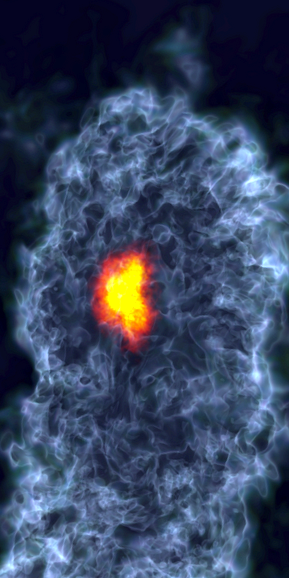
\includegraphics[width=0.875in]{PopIII_vr-edit.png}}
    \centerline{\tiny {[ Sam Skillman, Matt Turk ]}}
\end{minipage}
\end{frame}

  % Why does Enzo-P exist?
%======================================================================
\NEWSEC
%======================================================================

\subsection{\ssAmr}

%----------------------------------------------------------------------

\begin{frame}[fragile,label=ss-amr] 
\secframetitle{\ssAmr}
\begin{center}
\begin{minipage}{1in}
   \includegraphics<1->[width=1in]{enzo-sedov.png}
\end{minipage} \ 
\begin{minipage}{2.5in}
\blockblue
\begin{block}<+->{\textbf{\enzo}}
Structured AMR \\
Variable shaped patches \\
Neighbors \& parent communication
  \end{block}
\end{minipage} \\
\vspace{0.1in}
\begin{minipage}{1in}
   \includegraphics<2->[width=1in]{cello-sedov.png}
\end{minipage} \ 
\begin{minipage}{2.5in}
\blockgreen
   \begin{block}<+->{\textbf{\enzopcello}}
Array of octrees \\
Fixed shaped blocks \\
neighbors only communication
   \end{block}
\end{minipage}
\end{center}

\end{frame}

%----------------------------------------------------------------------

\begin{frame}[fragile] 
\secframetitle{\ssAmr}
\blockblue
\begin{block}<+->{\textbf{\enzo\ AMR}}
\begin{center}
\begin{minipage}{2.5in}
   \includegraphics<1->[width=2.5in]{enzo-amr.pdf}
\end{minipage}
\end{center}
\end{block}
\vspace{-0.2in}
\blockgreen
\begin{block}<+->{\textbf{\cello\ AMR}}
\begin{center}
\begin{minipage}{2.5in}
   \includegraphics<2->[width=2.5in]{cello-amr.pdf}
\end{minipage}
\end{center}
\end{block}
\end{frame}

         % How does Enzo-P's AMR compare to Enzo's
%======================================================================
\NEWSEC
%======================================================================

\subsection{\ssCompare}

\usebackgroundtemplate
{
\includegraphics[width=5in]{cello-background.png}}
\begin{frame}[fragile,label=ss-compare] 
% ----------------------------------------------------------------------
\secframetitle{\ssCompare}
%\framesubtitle{}
% ----------------------------------------------------------------------
\begin{center}
\rowcolors[]{1}{blue!5}{blue!10}
\begin{tabular}{l|cc} 
 & \textbf{\enzo} & \textbf{\enzopcello} \\ \hline
\uncover<2->{Parallelization} & \uncover<2->{MPI} & \uncover<2->{\charm} \\
\uncover<3->{AMR type}       & \uncover<3->{patch-based} & \uncover<3->{octree-based}   \\
\uncover<4->{AMR structure} & \uncover<4->{replicated} &\uncover<4->{ fully distributed}   \\
\uncover<5->{Time stepping} & \uncover<5->{level-adaptive} & \uncover<5->{block-adaptive$^*$}   \\
\uncover<6->{Block sizes} & \uncover<6->{$\times 1000$ variation} & \uncover<6->{constant}  \\
\uncover<7->{Task scheduling} & \uncover<7->{level-parallel} & \uncover<7->{dependency-driven}  \\
\uncover<8->{Load balancing} & \uncover<8->{patch migration} & \uncover<8->{\charm-based}  \\
\uncover<9->{Data locality} & \uncover<9->{LB conflict} & \uncover<9->{no LB conflict}  \\ 
\uncover<10->{Mesh quality} & \uncover<10->{level jumps} & \uncover<10->{2-to-1 constraint}  \\  \hline
\end{tabular} \\
\uncover<5->{\footnotesize $^*$ not implemented yet}
%  
% \ \\ \ \\
% \url{http://cello-project.org} \\
% NSF PHY-1104819, AST-0808184 \\
% $\qed$
\end{center}
\end{frame}

\usebackgroundtemplate
{}
     % What are the key differences between Enzo-P and Enzo?
%======================================================================
\NEWSEC
%======================================================================

\subsection{\ssApproach}

\begin{frame}[fragile,label=ss-approach] 
\secframetitle{\ssApproach}
\framesubtitle{\enzo's limitations}
%\framesubtitle{Scaling issues}
\begin{minipage}{3.0in}
%  AMR data structure scalability
%  Code development and maintenance
%  Ghost zone memory requirement
%  Patch size variation
%  Time stepping
%  Dynamic load balancing
%  Particle positions
%  Mesh quality
% So, how does Cello's AMR try to address the know issues of Enzo's current
% AMR?
%
% The main issues with Enzo's AMR design and implementation involve
% memory usage, the quality of the mesh, parallel task definition
% and scheduling, and data locality.

% [MEMORY] Memory usage is perhaps the most common limitation that
% people run into when running big Enzo simulations.  Enzo's mesh
% hierarchy structure is represented in each MPI process using a
% grid object for each AMR patch.  Although patches assigned to
% remote processors carry no field or particle data, the grid
% objects themselves still take up on the order of a few KB of memory.
% For small hierarchies that's not a problem, but when you have a million
% grid patches that means several GB of memory are required on each
% MPI process.  While supercomputers have gotten larger over the years, the
% amount of memory per node has not---it's still frequently just a few
% GB.  :  Memory fragmentation has also been identified as a problem,
% due to the high volume of heap memory new and delete operations on
% widely varying array sizes.  Ghost zone data can also consume a lot
% of memory, especially for smaller grids.

% [ MESH QUALITY ] Enzo also has known mesh quality issues.  Sometimes
% patches are adjacent to patches in refinement levels that are further than 
% a factor of two different. This can lead to inaccurate interpolation
% compromizing the numerical accuracy of solutions on such patches.

% [ PARALLEL TASKS ] Parallel tasks in Enzo are defined as a grid
% object and its associated field and particle data.  Patch sizes in
% Enzo can vary widly, from large $64^3$ root grid tiles to small
% $8^3$ patches on the finest levels.  Varying task sizes can
% adversely affect performance and load balancing.

\begin{itemize}
\item \bfat{2}{\textcolor{red!50!black}{Memory usage}}
\begin{itemize}
  \item<2-> \textcolor{red}{AMR structure is non-scalable}
  \item<2-> \textcolor{red}{memory fragmentation}
  \item<2-> \textcolor{red}{ghost zones}
\end{itemize}
\item \bfat{3}{\textcolor{green!50!black}{Mesh quality}}
\begin{itemize}
   \item<3-> \textcolor{green!80!black}{2-to-1 refinement constraint violated}
\end{itemize}
\item \bfat{4}{\textcolor{blue!50!black}{Parallel task definition}}
\begin{itemize}
   \item<4-> \textcolor{blue}{widely varying patch sizes}
   \item<4-> \textcolor{blue}{sizes determined by AMR}
\end{itemize}
\item \bfat{5}{\textcolor{cyan!50!black}{Parallel task scheduling}}
\begin{itemize}
   \item<5-> \textcolor{cyan!80!black}{parallel within a level}
   \item<5-> \textcolor{cyan!80!black}{synchronization between level time steps}
\end{itemize}
\item \bfat{6}{\textcolor{orange!50!black}{Data locality}}
\begin{itemize}
   \item<6-> \textcolor{orange!80!black}{disrupted by load balancing}
\end{itemize}
\end{itemize}
\end{minipage} \
\begin{minipage}{1.0in}
\centerline{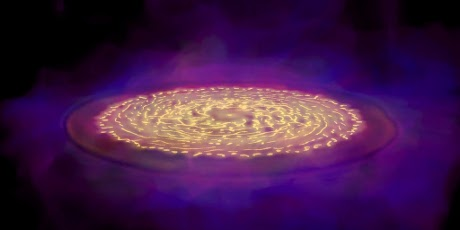
\includegraphics[width=2.0in,angle=90]{iso_and_volume_02_sm.jpg}}
\centerline{\tiny{[ Elizabeth Tasker ]}}
\end{minipage}
\end{frame}

%--------------------------------------------------

\begin{frame}[fragile] 
\secframetitle{\ssApproach}
\framesubtitle{\enzopcello\ approach}
%\framesubtitle{Scaling issues}
\begin{minipage}{3.0in}
%  AMR data structure scalability
%  Code development and maintenance
%  Ghost zone memory requirement
%  Patch size variation
%  Time stepping
%  Dynamic load balancing
%  Particle positions
%  Mesh quality
\begin{itemize}
\item \bfat{2}{\textcolor{red!50!black}{Memory usage}}
\begin{itemize}
  \item<2-> \textcolor{red}{AMR structure is fully distributed}
  \item<2-> \textcolor{red}{uniform blocks reduce fragmentation}
  \item<2-> \textcolor{red}{ghost zones allocated when needed$^*$}
\end{itemize}
\item \bfat{3}{\textcolor{green!50!black}{Mesh quality}}
\begin{itemize}
   \item<3-> \textcolor{green!80!black}{2-to-1 refinement constraint maintained}
\end{itemize}
\item \bfat{4}{\textcolor{blue!50!black}{Parallel task definition}}
\begin{itemize}
   \item<4-> \textcolor{blue}{uniform field array sizes in blocks}
   \item<4-> \textcolor{blue}{sizes determined by user}
\end{itemize}
\item \bfat{5}{\textcolor{cyan!50!black}{Parallel task scheduling}}
\begin{itemize}
   \item<5-> \textcolor{cyan!80!black}{asynchronous, data-driven}
   \item<5-> \textcolor{cyan!80!black}{block-local time stepping$^*$}
\end{itemize}
\item \bfat{6}{\textcolor{orange!50!black}{Data locality}}
\begin{itemize}
   \item<6-> \textcolor{orange!80!black}{only nearest-neighbor communication}
\end{itemize}
\end{itemize}
\vspace{-0.1in}
\only<1>{\textcolor{white}{\footnotesize $^*$ not implemented yet}}
\only<2-4>{\textcolor{red}{\footnotesize $^*$ not implemented yet}}
\only<5-6>{\textcolor{cyan!80!black}{\footnotesize $^*$ not implemented yet}}
\end{minipage} \
\begin{minipage}{1.0in}
\vspace{-0.2in}
\centerline{\tiny{Enzo}} 
\vspace{0.1in}
\centerline{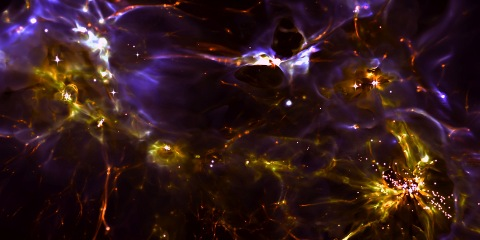
\includegraphics[width=2.0in,angle=90]{jhw-dwarf-galaxies.jpg}}
\centerline{\tiny{[ John Wise ]}}
\end{minipage}
\end{frame}

% ----------------------------------------------------------------------
    % How does Enzo-P AMR address Enzo's limitations?}
%======================================================================
\NEWSEC
%======================================================================

\subsection{\ssIntroSummary}

%----------------------------------------------------------------------

\begin{frame}[fragile,label=ss-intro-summary] 
\secframetitle{\ssIntroSummary}

\begin{itemize}
\item Enzo has awesome physics capabilities
\item Enzo also has fast and expertly-crafted numerical methods
\item Main limitations involve underlying data structures
  \begin{itemize}
  \item designed for 1990's supercomputers
  \item hierarchy memory limits scalability
  \item some mesh quality issues
  \end{itemize}
\item \bluetext{Cello} is designed to be a scalable AMR framework
  \begin{itemize}
  \item Charm++ data-driven asynchronous parallelism
  \item scalable forest-of-octree AMR
  \end{itemize}
\item \greentext{Enzo-P} combines Enzo's physics with Cello's AMR
\end{itemize}
\vfill
\centerline{$\qed$}
\end{frame}




  %======================================================================
\NEWMOD
%======================================================================

\section{\sPresent}

%----------------------------------------------------------------------

\logo{\hfill\hyperlink{outline<1>}{\icon}}

\begin{frame}[fragile,label=s-present] 
\modframetitle{\sPresent}
\small
\begin{center}
\begin{minipage}{3.25in}
\begin{enumerate}
\item \hyperlink{ss-state<1>}   {\BUTTON {\ssState}}
\item \hyperlink{ss-current<1>}   {\BUTTON {\ssCurrent}}
\item \hyperlink{ss-scaling<1>}   {\BUTTON {\ssScaling}}
\item \hyperlink{ss-issues<1>}   {\BUTTON {\ssIssues}}
\item \hyperlink{ss-present-summary<1>}   {\BUTTON {\ssPresentSummary}}
\end{enumerate}
\end{minipage}
\end{center}
\end{frame}

\logo{\hfill\hyperlink{s-present<1>}{\icon}}

%======================================================================
\NEWSEC
%======================================================================

\subsection{\ssState}

\begin{frame}[fragile,label=ss-state] 

\secframetitle{\ssState}

%  What is the current state of Enzo-P?  Well, it can do this.

%  This is a pure hydrodynamics problem run using Enzo-P with AMR
%  enabled, with somewhat non-physical initial conditions.

%  It uses an ``array of octrees'' AMR approach, which is simply a
%  uniform array of octrees.  Each Block in the hierarchy contains a
%  small grid of field variables, with size typically around 16^3 to
%  32^3.

%  Enzo-P is parallelized using Charm++ instead of MPI.  Charm++ is an
%  asynchronous data-driven parallel programming language extention to
%  C++.  Each block in the mesh hierarchy is a separate parallel task
%  in Charm, called called a ``chare''.  A key feature of Cello's AMR
%  Charm++ implementation is that it is fully distributed--there is
%  *no* hierarchy meta-data, which addresses a key limitation of
%  the current Enzo.

%  Enzo-P is also designed to be powerful yet easy to use.  While you
%  *can* implement test problem types in Enzo-P like you can Enzo, you
%  can also specify initial and boundary conditions directly in the
%  parameter file.  In this example, initial conditions were generated
%  using a PNG file as a logical mask---the density is initialized to
%  1.5 wherever the PNG file pixels are non-black, otherwise its set
%  to be 12 times less.  This approach means that common test problems
%  such as the implosion problem, Sedov blast wave, or double mach
%  reflection can be set up in the parameter file exclusively without
%  requiring any C++ coding.

\pause
\begin{center}
\begin{minipage}{4.5in}
\begin{minipage}{2.9in}
\only<2->{\vspace{-0.1in}\centerline{in 2014} \ \\ \vspace{-0.2in} \ANIMATEGRAPHICS{width=2.9in}{10}{Images/Daze/daze-0}{000}{100}}
\end{minipage} \ 
\begin{minipage}{1.45in}
\only<3->{\vspace{-0.1in}\centerline{in 2015} \ \\ \vspace{-0.2in}\ANIMATEGRAPHICS{width=1.45in}{10}{Images/1509/1509-0}{00}{56}}
\end{minipage}
\end{minipage}
\end{center}
\pause
\pause
\begin{minipage}[t]{1.2in}
\footnotesize
\vspace{0.1in}
\blockred
\begin{block}<+->{\textbf{Mesh refinement}}
\scriptsize
 \mbox{``array-of-octrees''} \\
 \mbox{field data on blocks} \\ \ \\
\end{block}
\end{minipage} \ \ 
\begin{minipage}[t]{1.0in}
\footnotesize
\vspace{0.1in}
\blockgreen
\begin{block}<+->{\textbf{Parallelism}}
\scriptsize
 Charm++\\
\mbox{blocks are ``chares''} \\
 \mbox{fully-distributed}
\end{block}
\end{minipage} \ \
\begin{minipage}[t]{1.6in}
\raggedright
\footnotesize
\vspace{0.1in}
\blockblue
\begin{block}<+->{\textbf{Parameters}}
\scriptsize
 \mbox{\code{Initial \{ density \{}} \\
 \mbox{\code{ value = [ 1.5, "daze.png",  }} \\
 \mbox{\code{\ \ \ \ \ \ \ \ \ \ \ 0.125 ]; \} \} }}
\end{block}
\end{minipage}

\end{frame}

%----------------------------------------------------------------------

\begin{frame}[fragile,label=ss-state] 
\secframetitle{\ssState}
\begin{center}
\begin{minipage}{4.5in}
\begin{minipage}{2.2in}
\only<2->{\centerline{in 2016}}
\end{minipage}
\begin{minipage}{2.2in}
\only<3->{\centerline{in 2017}}
\end{minipage}
 \vspace{0.2in} \\
\begin{minipage}{2.2in}
\begin{center}
\only<2->{\ANIMATEGRAPHICS{width=1.8in}{10}{trace-}{00}{99}}
\end{center}
\end{minipage} \
\begin{minipage}{2.2in}
\only<3->{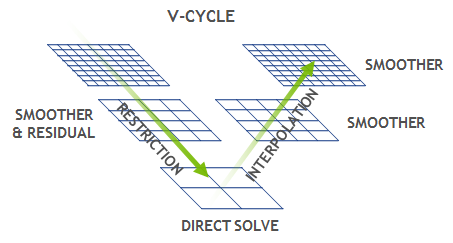
\includegraphics[width=2.0in]{hpgmg_v_cycle.png}}
\end{minipage}
\end{minipage}
\end{center}
\end{frame}

%----------------------------------------------------------------------

\begin{frame}[fragile,label=ss-state] 
\secframetitle{\ssState}
\begin{center}
\centerline{in 2018}  \ \\
\begin{minipage}{4.5in}
\begin{minipage}{2.2in}
\only<2->{\ANIMATEGRAPHICS{width=2.0in}{5}{Images/Cosmo/B3/dark-}{00}{21}}
\end{minipage} \
\begin{minipage}{2.2in}
\only<3->{\ANIMATEGRAPHICS{width=2.0in}{5}{Images/Cosmo/B3/mesh-}{00}{21}}
\end{minipage}
\end{minipage}
\end{center}
\end{frame}

  % What is the current state of Enzo-P/Cello?
%======================================================================
\NEWSEC
%======================================================================

\subsection{\ssCurrent}

% ----------------------------------------------------------------------
\begin{frame}[fragile,label=ss-current] 
\secframetitle{\ssCurrent}

\rowcolors[]{1}{blue!5}{blue!10}
\begin{tabular}{ll}
\uncover<2->{\erow{Physics}} &
\uncover<2->{\erow{PPM, \magentabf{scalable} gravity, (grackle), \magentabf{cosmology}}} \\

\uncover<3->{\orow{Field data}} &
\uncover<3->{\orow{(padding, alignment, precision, centering)}} \\

\uncover<4->{\erow{Particle data}} &
\uncover<4->{\erow{(types, attributes, batches, constants)}} \\

\uncover<5->{\orow{Initial conditions}} &
\uncover<5->{\orow{direct ($f(x,y,z)$), problems (Implosion, Sedov)}} \\

\uncover<6->{\erow{Boundary conditions}} &
\uncover<6->{\erow{inflow ($f(x,y,z,t)$), outflow, reflecting, periodic}} \\

\uncover<7->{\orow{Refinement criteria}} &
\uncover<7->{\orow{slope, density, shear, shock, \magentabf{mass}}} \\

\uncover<8->{\erow{Interpolation}} &
\uncover<8->{\erow{linear, \textcolor{gray}{\enzo's \textit{SecondOrderA}, etc.}}} \\

\uncover<9->{\orow{Time stepping}} &
\uncover<9->{\orow{uniform, \textcolor{gray}{level-adaptive}, \textcolor{gray}{block-adaptive}}} \\

\uncover<10->{\erow{Checkpoint/restart}} &
\uncover<10->{\erow{\charm\ (disk, memory+disk)}} \\

\uncover<11->{\orow{Load balancing}} &
\uncover<11->{\orow{\charm\ (dozens of strategies available)}} \\

\uncover<12->{\erow{I/O}} &
\uncover<12->{\erow{\textcolor{gray}{scalable} HDF5, PNG}} \\
\end{tabular}
\ \\
\ \\
\ \\
\centerline{
\uncover<1->{\magentatext{New capability}} \hfill
\uncover<1->{\bluetext{Pre-existing capability}} \hfill
\uncover<1->{\textcolor{gray}{Not ready yet}}}
\end{frame}
  % What are Enzo-P's current and near future capabilities?
%======================================================================
\NEWSEC
%======================================================================

\subsection{\ssScaling}

\begin{frame}[fragile,label=ss-scaling] 
\secframetitle{\ssScaling}
\begin{center}
\begin{minipage}{4.50in}
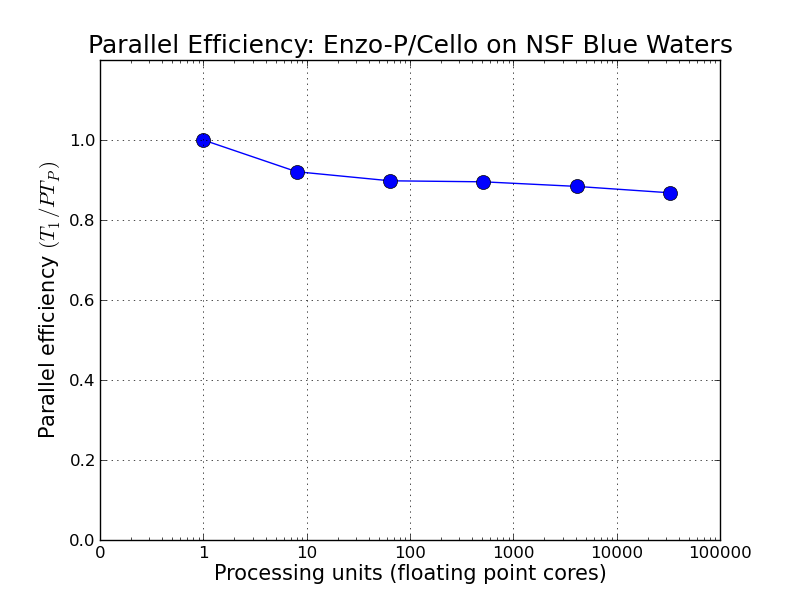
\includegraphics[width=2.25in]{scale-eff.png} \ 
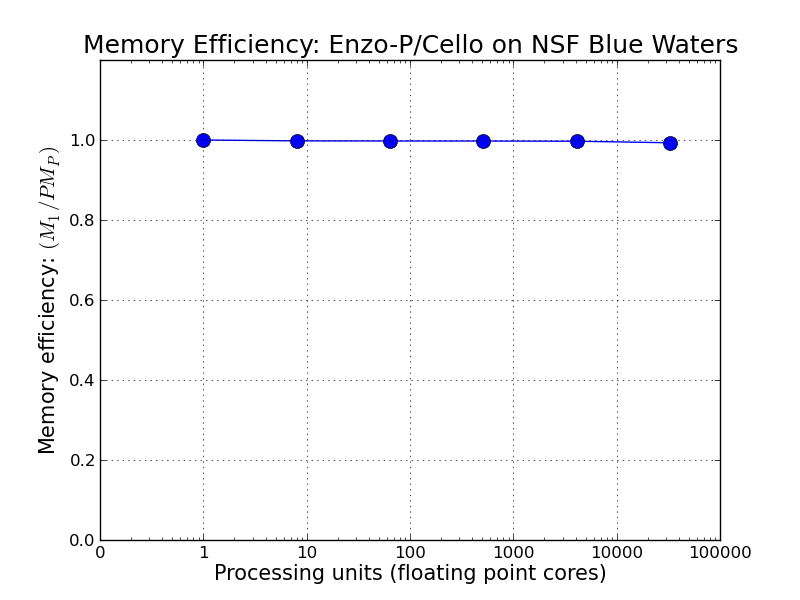
\includegraphics[width=2.25in]{scale-mem.png}
\end{minipage} \\
\begin{minipage}{4.0in}
\footnotesize
\pause
\begin{minipage}[t]{1.20in}
\blockblue
\begin{block}<+->{Problem}
%\begin{itemize}
Sedov blast array \\
$L=3$; $32K$ cores \\
$32^3$ cells / block \\
$329$ blocks /core
%\end{itemize}
\end{block}
\end{minipage} \
\begin{minipage}[t]{1.20in}
\blockgreen
\begin{block}<+->{Parallel Efficiency}
%\begin{itemize}
\begin{tabbing}
xxxxxxxxxx\=\kill
Time \> $0.868$ \\
Memory \> $0.993$
\end{tabbing}
%\end{itemize}
\end{block}
\end{minipage} \
\begin{minipage}[t]{1.20in}
\blockred
\begin{block}<+->{Caveats}
%\begin{itemize}
load balanced \\
few refinement steps \\
startup ignored
%\end{itemize}
\end{block}
\end{minipage}
\end{minipage}
\end{center}
\end{frame}

  % How well does ENzo-P scale?
%======================================================================
\NEWSEC
%======================================================================

\subsection{\ssIssues}

\begin{frame}[fragile,label=ss-issues] 
\secframetitle{\ssIssues}
\framesubtitle{Parameter file issues}
% Review ss-bugs.tex / http://client64-249.sdsc.edu/cello-bug

\begin{itemize}
   \item Floats and ints cannot be mixed
   \cornersize{0.9}
   \begin{itemize}
     \item[\frownie] \textcolor{red}{\code{velocity\_x = 8.0 + 2*x }}
     \item[\smiley] \textcolor{green!50!black}{\code{velocity\_x = 8.0 + 2.0*x}}
   \end{itemize}

   \item Need space after subtraction minus sign
   \begin{itemize}
     \item[\frownie] \textcolor{red}{\code{density = x -2.0;}}
     \item[\smiley] \textcolor{green!50!black}{\code{density = x - 2.0;}}
   \end{itemize}
  \item Need at least as many root blocks as processors $P$
  \begin{itemize}
    \item \code{Mesh \{ root\_blocks = [4,4,4]; \} }
    \item[\frownie] \textcolor{red}{\code{\$ charmrun +p72} \code{bin/enzo-p \ldots}}
    \item[\smiley]\textcolor{green!50!black}{\code{\$ charmrun +p64} \code{bin/enzo-p \ldots}}
  \end{itemize}
  \item AMR requires ghost zone depth of $\ge 4$
\end{itemize}

\link{ss-bugs}{Other issues: see bug tracking website}

\end{frame}
      % What are some of Enzo-P's known issues?
%======================================================================
\NEWSEC
%======================================================================

\subsection{\ssPresentSummary}

%----------------------------------------------------------------------

\begin{frame}[fragile,label=ss-present-summary] 
\secframetitle{\ssPresentSummary}
\begin{itemize}
\item Enzo-P / Cello now includes gravity as well as hydro
\item (Still only fields, but particles coming very soon)
\item Checkpoint/restart now working
\begin{itemize}
\item ``free'' via \charm
\item checkpoint to file or remote memory
\item automatic fault tolerance possible
\end{itemize}
\item Dynamic load balancing now available
\begin{itemize}
\item ``free'' via \charm
\item dozens of sophisticated schemes available
\end{itemize}
\item Several new refinement criteria implemented
\item Parallel scaling is very promising
\item Codebase could still use some improvement
\end{itemize}
\vfill
\centerline{$\qed$}
\end{frame}



  %======================================================================
\NEWMOD
%======================================================================

\section{\sRecent}

\logo{\hfill\hyperlink{outline<1>}{\icon}}

%----------------------------------------------------------------------

\begin{frame}[fragile,label=s-recent] 
\modframetitle{\sRecent}
\small
\begin{center}
\begin{minipage}{3.25in}
\begin{enumerate}
\item \hyperlink{ss-recent-particles<1>}   {\BUTTON {\ssRecentParticles}}
\item \hyperlink{ss-recent-gravity<1>}     {\BUTTON {\ssRecentGravity}}
\item \hyperlink{ss-recent-history<1>}     {\BUTTON {\ssRecentHistory}}
\item \hyperlink{ss-recent-units<1>}       {\BUTTON {\ssRecentUnits}}
\item \hyperlink{ss-recent-cosmology<1>}       {\BUTTON {\ssRecentCosmology}}
\end{enumerate}
\end{minipage}
\end{center}
\end{frame}

\logo{\hfill\hyperlink{s-recent<1>}{\icon}}

%======================================================================
\NEWSEC
%======================================================================

\subsection{\ssRecentParticles}

%----------------------------------------------------------------------
\begin{frame}[fragile,label=ss-recent-particles] 
  \secframetitle{\ssRecentParticles}
  \framesubtitle{Cello supports Particles!}

\begin{minipage}{2.5in}
\begin{itemize}
\item user-defined types
\begin{itemize}
        \item  declared in input parameter file
        \item  \bluecode{"trace"}: tracer particles
        \item  \bluecode{"dark"}: dark matter particles
        \item  others defined as needed
\end{itemize}
\item each with own list of attributes
\begin{itemize}
        \item  position (\bluecode{"x"},\bluecode{"y"},\bluecode{"z"})
        \item  velocity (\bluecode{"vx"},\bluecode{"vy"},\bluecode{"vz"})
        \item  mass (\bluecode{"mass"})
        \item  id (\bluecode{"id"})
        \item \textit{integer} (8-,16-,32-,64-bit)
        \item \textit{float}   (32-, 64-, 128-bit)
        \end{itemize}
\item constant attributes available
\end{itemize}
\end{minipage} \
\begin{minipage}{2.0in}
%\ANIMATEGRAPHICS{width=1.25in}{20}{Images/Trace/Trace-0}{000}{010}
\end{minipage}
\end{frame}

%======================================================================

\begin{frame}[fragile,label=ss-recent-particles] 
  \secframetitle{\ssRecentParticles}
\framesubtitle{How \code{Particle} objects store particle data}
\begin{minipage}{1.8in}
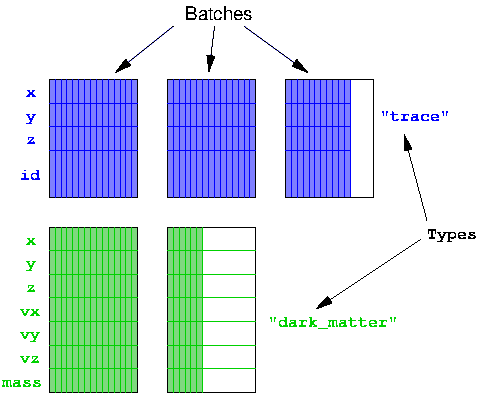
\includegraphics[width=2.0in]{particles-design.pdf} \ \\
\end{minipage} \ 
\begin{minipage}{2.5in}
\begin{itemize}
\item multiple particle \textit{types}
\item particles allocated in \textit{batches}
\begin{itemize}
\item fixed size arrays
\item fewer new/delete operations
\item efficient insert/delete operations
\item potentially useful for GPU's
\end{itemize}
\item batches store particle \textit{attributes}
\begin{itemize}
\item (position, velocity, mass, etc.)
\item 8,16,32,64-bit integers
\item 32,64,128-bit floats
\end{itemize}
\end{itemize}
\end{minipage}
\begin{itemize}
\item particle positions may be floating-point or integers
\begin{itemize}
\item floating-point for storing global positions
\item integers for \code{Block}-local coordinates
\begin{itemize}
\item solves reduced precision issue for deep hierarchies
\item less memory required for given accuracy
\end{itemize}
\end{itemize}
\end{itemize}
\end{frame}

%----------------------------------------------------------------------
%
% Review of Particles in Cello
%
%   Particles that move between blocks are handled by Cello
%
%   Cello handles moving particles
%     4^3 array
%     one-pass through particles to sort and scatter
%     particles
%

\begin{frame}[fragile,label=ss-recent-particles] 
  \secframetitle{\ssRecentParticles}
  \framesubtitle{Particle communication between Blocks}
\begin{itemize}
\item communication is required when particles move outside a Block 
\item this is done using a 4x4x4 array
\begin{itemize}
\item array contains pointers to ParticleData (PD) objects
\item one PD object per neighbor Block
\end{itemize}

\end{itemize}
\begin{minipage}{1.8in}
%\includegraphics<1>[width=2.0in]{particle-refresh-0.pdf}
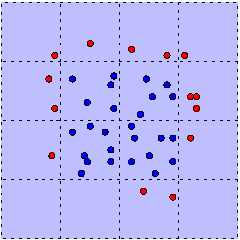
\includegraphics[width=2.0in]{particle-refresh-2.pdf}
%\includegraphics<4>[width=2.0in]{particle-refresh-3.pdf}
%\includegraphics[width=2.0in]{particle-refresh-4.pdf}
\end{minipage} \ 
\begin{minipage}{2.7in}
\begin{itemize}
\item migrating particles are
\begin{itemize}
\item \code{scatter()}-ed to PD array objects
\item sent to associated neighbors
\item \code{gather()}-ed by neighbors
\end{itemize}
\item one sweep through particles
\item one communication step per neighbor
%\item similar for refinement / coarsening
\end{itemize}
\end{minipage}
\end{frame}

%----------------------------------------------------------------------
%  
%   Class structure of particles in Cello mirrors Field classes
%
%   Particle: particles as seen by application
%     ParticleDescr: ``descriptor'' class defining particle parameters
%     ParticleData: ``data'' class containing block particle data
%

%\begin{frame}[fragile,label=ss-recent-particles] 
%  \secframetitle{\ssRecentParticles}
%  \framesubtitle{Class structure of particles}
%
%\end{frame}

%----------------------------------------------------------------------

\begin{frame}[fragile,label=ss-recent-particles] 
  \secframetitle{\ssRecentParticles}
  \framesubtitle{Particle type parameters}
Particles are declared in the input parameter file using the Particle group

\begin{tabbing}
\code{xxxxxx}\=\code{xxxxx}\=\code{xxxxxxxxxxxxxx}\=\kill
\code{Particle \{} \\
\>    \code{list = ["trace"];} \\
\\
\>    \code{trace \{} \\
\> \>     \code{attributes = ["id", "int64",} \\
\> \> \> \code{\ "x", "single",} \\
\> \> \> \code{\ "y", "single",} \\
\> \> \> \code{\ "z", "single"];} \\
\> \>      \code{position = ["x","y","z"];} \\
\> \>      \code{batch\_size = 2000; } \\
\>    \code{\} } \\
\code{\} }
\end{tabbing}
\end{frame}

%----------------------------------------------------------------------

\begin{frame}[fragile,label=ss-recent-particles] 
  \secframetitle{\ssRecentParticles}
  \framesubtitle{Particle type parameters}
  \small
\begin{tabbing}
\code{xx}\=\code{xx}\=\code{xxx}\=\kill
\code{Particle \{} \\
\>    \code{list += ["dark"];} \\
\\
\>    \code{dark \{ } \\
\> \> 	  \code{attributes = } \\
\> \> \> \code{  [ "x", "double",  "y", "double", "z", "double",} \\
\> \> \> \code{   "vx", "single", "vy", "single","vz", "single",} \\
\> \> \> \code{   "ax", "single", "ay", "single","az", "single"];} \\
\> \>     \code{constants = ["mass", "single"];} \\
\> \>     \code{position = [ "x", "y", "z"];} \\
\> \>     \code{velocity = ["vx","vy","vz"];} \\
\> \>     \code{groups = ["has\_mass"];} \\
\>      \code{\} } \\ 
\code{\} }
\end{tabbing}
\end{frame}
%----------------------------------------------------------------------
%  Runs were made with tracer particles to ensure parallel scaling
%
%
%   - [ ]  include 1705-BW slides
%

\begin{frame}[fragile,label=ss-recent-particles] 
  \secframetitle{\ssRecentParticles}
  \framesubtitle{Parallel scaling test problem}
  \textbf{We tested basic \enzop\ hydrodynamics and particles scalability}
  \begin{minipage}{1.5in}
  \vspace{0.2in}
    \includegraphics<1>[width=1.5in]{de-2-3.png} \\
\ \\
    \includegraphics<1>[width=1.5in]{age-2-16.png}
  \end{minipage} \
  \begin{minipage}{2.75in}
    \vspace{0.1in}
    \begin{itemize}
    \item variation of ``array of Sedov Blast'' test
    \item letters instead of spheres
      \begin{itemize}
      \item inhibits lockstep coarsen/refine
      \end{itemize}
    \item one letter per Blue Waters core
    \item tested with/without tracer particles
    \item $32^3$ or $24^3$ cells per block
    \item among largest AMR runs ever done
      \begin{itemize}
      \item $256K$ fp-cores
      \item $1.7T$ cells; $0.7T$ (cells + particles)
        \item $50M$ Blocks
      \end{itemize}
      \item \enzo\ would require $ \ge 72GB$ / process
    \end{itemize}
    \end{minipage}
  
\end{frame}

\begin{frame}[fragile,label=ss-recent-particles] 
  \secframetitle{\ssRecentParticles}
  \framesubtitle{Particle weak scaling results}
%--------------------------------------------------  
\begin{center}
  \vspace{-0.1in}
  \begin{minipage}{4.50in}
    \begin{center}
%      \begin{minipage}{2in}
%    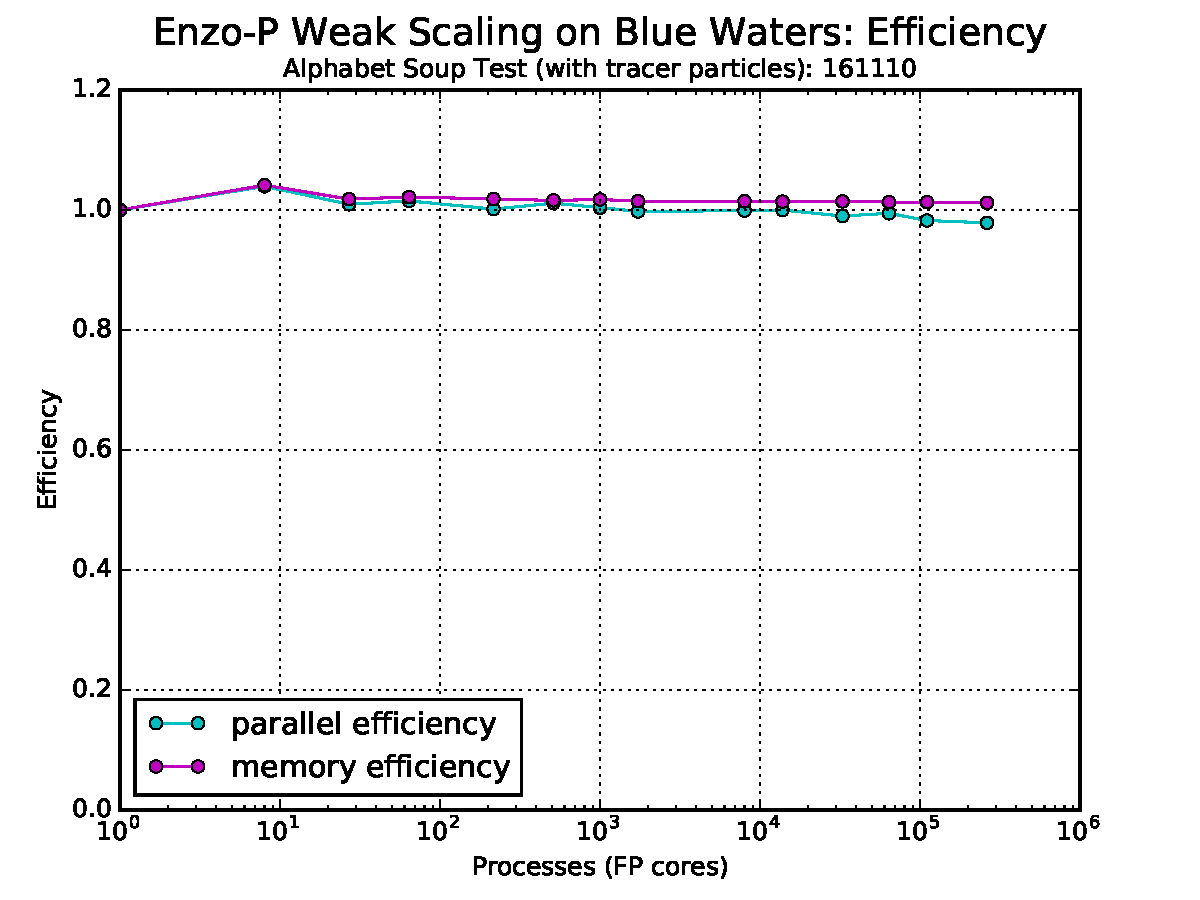
\includegraphics[width=2.0in]{scaling-efficiency-161110.pdf}
%    \end{minipage} \ 
      \begin{minipage}{4in}
    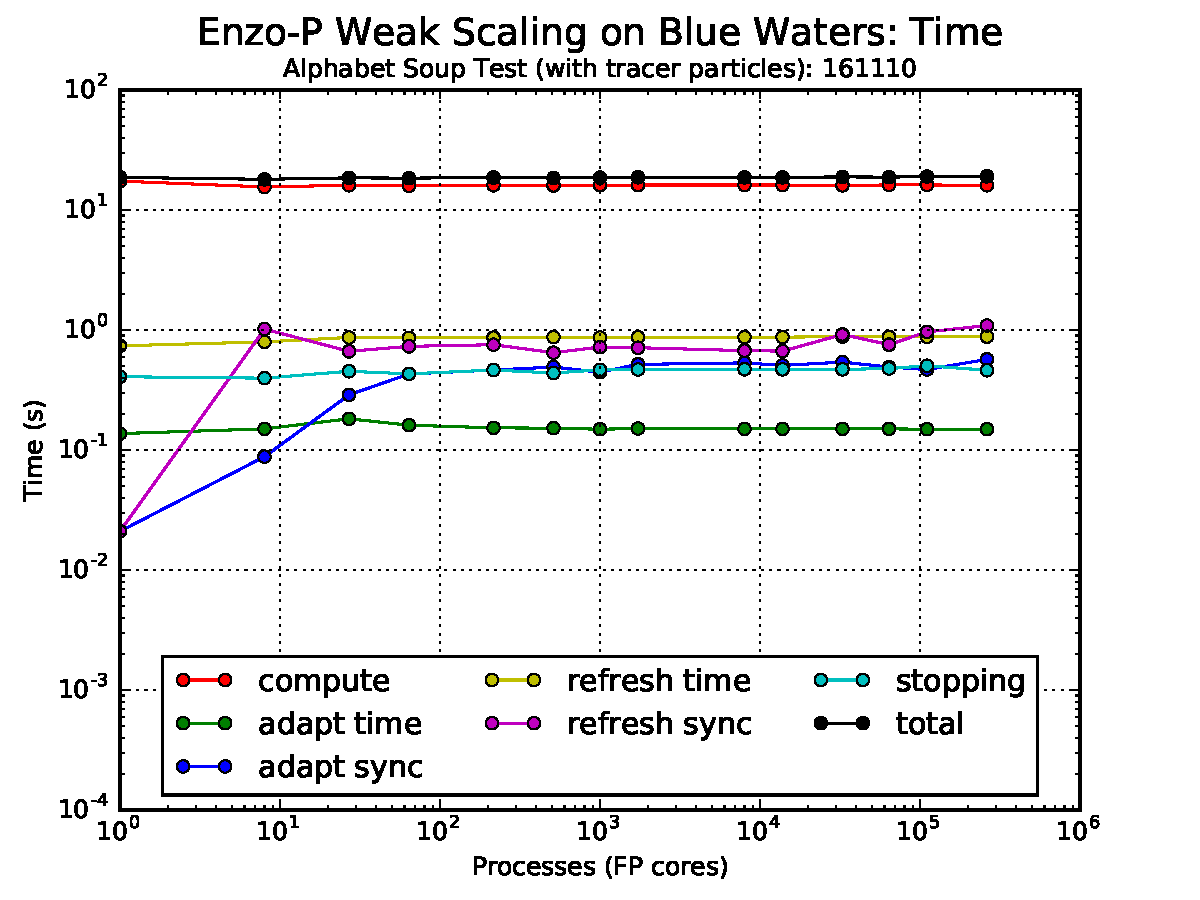
\includegraphics[width=4.0in]{scaling-time-161110.pdf}
    \end{minipage} \\
    \end{center}
  \end{minipage} \\
\end{center}
  
\end{frame}


 %
%======================================================================
\NEWSEC
%======================================================================

%   - [ ] Collapse demonstration (tracer particles)
%
%   - [ ] List of gravity-related capabilities
%
%     dark matter particles
%     CIC particle deposit into "total density" field
%     scalable linear solver
%        multigrid: unigrid working
%        Reynolds "HG"
%            one last final bug cornered
%            [ images ]
%     KDK particle updates
%        todo--use t + 0.5*dt for updates
%     
%   - [ ] How gravity code is organized
%
%     EvolveLevel
%      :458 PrepareDensityField 
%           pm_deposit
%  	 gravity if level == 0
%      :495 SolveForPotential
%           gravity if level > 0
%      :497 ComputeAccelerations
%      :539 SolveHydroEquations
%           update density fields
%      :548 UpdateParticlePositions
%           update particle positions
%
%   - [ ] How parameters files are defined
%
%
%      Method {
%         list = [ "pm_deposit", "gravity", "ppm", "pm_update" ];
%
%        pm_deposit { ... }
%        gravity { ... }
%           solver = "bicgstab"
%	ppm
%	pm_update
%	
%     Solver {
%        list = ["MG","BCG","J1","C","J2"];
%        MG {
%           type = "mg0";
%	   local = true;
%        }
%     }
%
%   - [ ] Code structure
%     code has (d)evolved to have multiple "levels" of Block computation
%     Method
%        general physics-based code
%        typically requires refresh of ghost zones
%        examples EnzoMethodPpm, EnzoMethodPpml, EnzoMethodGrackle
%        list = [...] specifies order of computation, as hard-coded 
%          in EvolveLevel
%     Solver [new]
%        solve or approximate solve of A*X = B
%        typically requires refresh of ghost zones
%        examples: EnzoSolverBiCgStab, EnzoSolverCg, EnzoSolverMg0,
%                  EnzoSolverJacobi
%        can composit solvers: BiCgStab + Mg0 + (Jacobi, Cg)
%        list = [ ... ] needs to include all solvers involved
%        - [ ] write solver-hg.incl, solver-mg0.incl, etc.
%     Compute 
%        local-only computation
%        typically don't require ghost zones
%        eg EnzoComputeTemperature, EnzoComputePressure
%
%   - [ ] Multigrid solver
%
%     EnzoSolverMg0
%     uses EnzoMatrixLaplace matvec
%     existing prolong and restrict
%
%     Parameters setup
%
%     sequencing: I'm in level 0 < k < N.  What do I do?
%
%       ( verify from code )
%
%         1. do nothing (finer grids start)
%         2. receive coarsened residual from a child
%	    2a. if not last child, do nothing
%            2b. if last child, continue
%	 3. pre-smooth
%	 4. send coarsened data to parent
%	 5. do nothing (coarser grids continue V-cycle)
%         6. receive correction from parent
%         7. prolong correction and update solution
%	 8. post-smooth
%         9. send correction to parent
%	10. last V-cycle iteration?
%	    if no, then do nothing
%	    if yes, then refresh
%
%   - [ ] Reynolds "HG" solver
%
%     description
%
%     equations
%
%     implementation in Enzo-P
%        bicgstab solver
%        mg0 preconditioner
%	mg0 no pre- or post-smoothing
%
%     parameters set up
%
%        Method {
%     
%   - [ ] Scaling results on Blue Waters
%
%     ( slides from BW talk)
%
%     Note V-cycle only
%        actual solves require O(log N)
%        FMG less scalable too--more work on coarser blocks
%
%     
%        
%   
%
%   
%   Method
%     pm_deposit
%       deposit particle mass into "density_total"
%     gravity [ rename?  e.g. potential ]
%       compute potential given "density_total"
%       compute accelerations
%
%     "ppm"
%     pm_update


\subsection{\ssRecentGravity}

\begin{frame}[fragile,label=ss-recent-gravity] 
\secframetitle{\ssRecentGravity}
\end{frame}

   %
%======================================================================
\NEWSEC
%======================================================================
% 
%  Recent
%  History of Fields
%
%----------------------------------------------------------------------
  

\subsection{\ssRecentHistory}

\begin{frame}[fragile,label=ss-recent-history] 
  \secframetitle{\ssRecentHistory}
  \framesubtitle{Cello supports field history}
  \begin{itemize}
  \item Specify history in parameter file

  Field {
     history = 1;
  }
  \end{itemize}
%  
%
%
%  Access arrays as usual, plus optional history parameter
%
%  Field field = enzo_block->data()->field();
%
%  int id = field.field_id ("density");
%
%  enzo_float * de_new = field.unknowns(id,0);
%  enzo_float * de_old = field.unknowns(id,1);
%
%  double time_new = enzo_block->time()
%  double time_old = field.history_time(1);
%
%  for (int iz=0; iz<nz; iz++) {
%    for (int iy=0; iy<ny; iy++) {
%      for (int ix=0; ix<nx; ix++) {
%         de_new[i] - de_old[i];
%       }
%    }
%  }

\end{frame}

 %
%======================================================================
\NEWSEC
%======================================================================

\subsection{\ssRecentUnits}

\begin{frame}[fragile,label=ss-module-section] 
\secframetitle{\ssRecentUnits}
\end{frame}

 %
%======================================================================
\NEWSEC
%======================================================================

\subsection{\ssRecentCosmology}

\begin{frame}[fragile,label=ss-recent-cosmology] 
\secframetitle{\ssRecentCosmology}
\begin{itemize}
\item Block size $32^3$
\end{itemize}
\begin{center}
\begin{minipage}{2.0in}
\only<1->{\ANIMATEGRAPHICS{width=2.0in}{05}{Images/Comet-run.34/dark-}{00}{33}}
\end{minipage} \ 
\begin{minipage}{2.0in}
\only<1->{\ANIMATEGRAPHICS{width=2.0in}{05}{Images/Comet-run.34/mesh-}{00}{33}}
\end{minipage}
\end{center}
\end{frame}

%----------------------------------------------------------------------

\begin{frame}[fragile,label=ss-recent-cosmology] 
\secframetitle{\ssRecentCosmology}
\begin{itemize}
\item Block size $16^3$
\end{itemize}
\begin{center}
\begin{minipage}{2.0in}
\only<1->{\ANIMATEGRAPHICS{width=2.0in}{05}{Images/Comet-run.35/dark-}{00}{26}}
\end{minipage} \ 
\begin{minipage}{2.0in}
\only<1->{\ANIMATEGRAPHICS{width=2.0in}{05}{Images/Comet-run.35/mesh-}{00}{26}}
\end{minipage}
\end{center}
\end{frame}

%----------------------------------------------------------------------


\begin{frame}[fragile,label=ss-recent-cosmology] 
\secframetitle{\ssRecentCosmology}
\begin{itemize}
\item Block size $8^3$
\end{itemize}
\begin{center}
\begin{minipage}{2.0in}
\only<1->{\ANIMATEGRAPHICS{width=2.0in}{05}{Images/Comet-run.36/dark-}{00}{21}}
\end{minipage} \ 
\begin{minipage}{2.0in}
\only<1->{\ANIMATEGRAPHICS{width=2.0in}{05}{Images/Comet-run.36/mesh-}{00}{21}}
\end{minipage}
\end{center}
\end{frame}


\begin{frame}[fragile,label=ss-recent-cosmology] 
\secframetitle{\ssRecentCosmology}
\centerline{Block size $32^3$ runs the fastest}
\begin{center}
\begin{minipage}{3.5in}
\only<1->{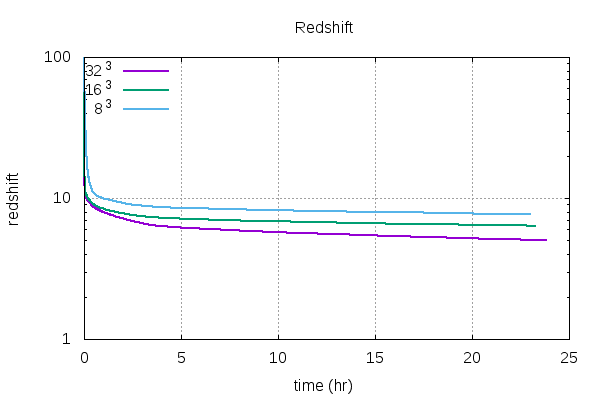
\includegraphics[width=3.5in]{Images/b345-redshift.png}}
\end{minipage} \ 
\end{center}
\end{frame}

\begin{frame}[fragile,label=ss-recent-cosmology] 
\secframetitle{\ssRecentCosmology}
\centerline{But block size $32^3$ uses the most memory}
\begin{center}
\begin{minipage}{3.5in}
\only<1->{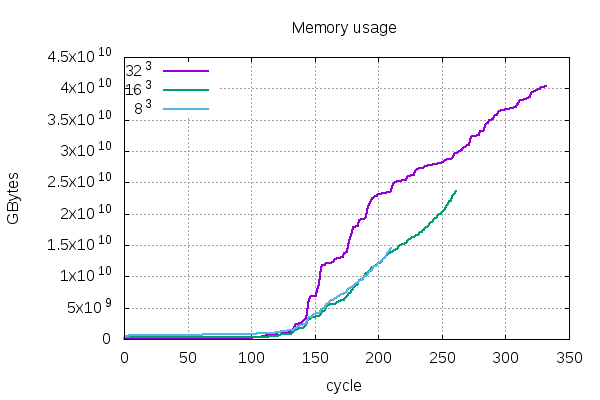
\includegraphics[width=3.5in]{Images/b345-bytes.png}}
\end{minipage} \ 
\end{center}
\end{frame}

\begin{frame}[fragile,label=ss-recent-cosmology] 
\secframetitle{\ssRecentCosmology}
\centerline{Time per cycle has a burst of growth at varying points}
\begin{center}
\begin{minipage}{3.5in}
\only<1->{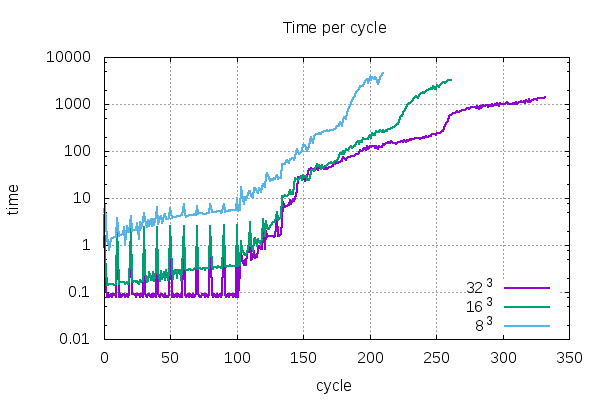
\includegraphics[width=3.5in]{Images/b345-time-per-cycle-log.png}}
\end{minipage}
\end{center}
\end{frame}

\begin{frame}[fragile,label=ss-recent-cosmology] 
\secframetitle{\ssRecentCosmology}
\centerline{Solver time scaled by number of blocks shows this even more}
\begin{center}
\begin{minipage}{3.5in}
\only<1->{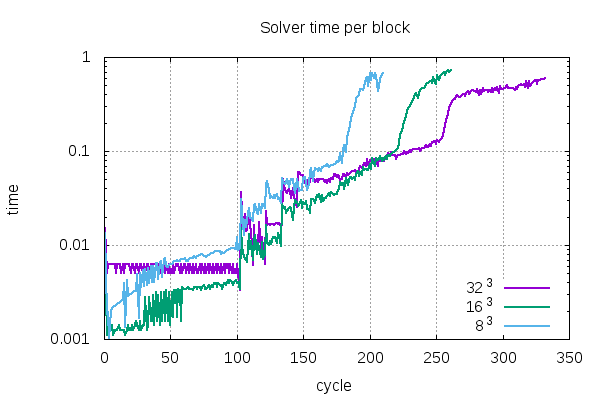
\includegraphics[width=3.5in]{Images/b345-time-per-block.png}}
\end{minipage}
\end{center}
\end{frame}

\begin{frame}[fragile,label=ss-recent-cosmology] 
\secframetitle{\ssRecentCosmology}
\centerline{Yet number of solver iterations is very reasonable}
\begin{center}
\begin{minipage}{3.5in}
\only<1->{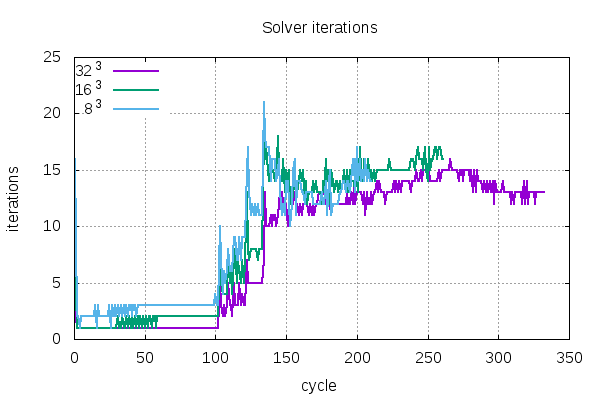
\includegraphics[width=3.5in]{Images/b345-bcg-iters.png}}
\end{minipage}
\end{center}
\end{frame}

\begin{frame}[fragile,label=ss-recent-cosmology] 
\secframetitle{\ssRecentCosmology}
\centerline{Memory per block is also increasing}
\begin{center}
\begin{minipage}{3.5in}
\only<1->{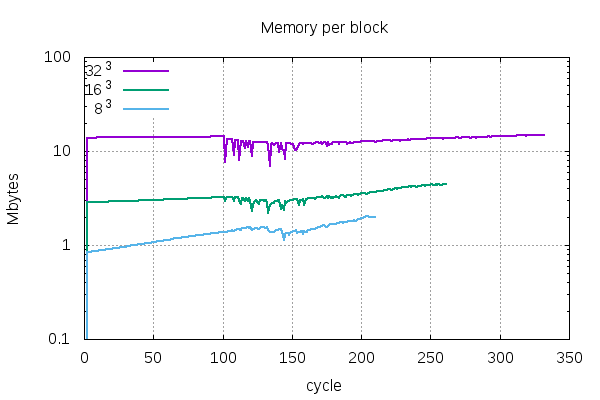
\includegraphics[width=3.5in]{Images/b345-bytes-per-block.png}}
\end{minipage}
\end{center}
\end{frame}

% \begin{frame}[fragile,label=ss-recent-cosmology] 
% \secframetitle{\ssRecentCosmology}
% Cosmological parameters are set in the \code{Physics} parameter group.
% \small
% \begin{tabbing}
% \code{xxx}\=\code{xxx}\=\code{xxx}\=\code{xxxxxxxxxxxxxxxxxxxxx}\=\kill
% \>\code{Physics \{ } \\
% \> \> \code{list = ["cosmology"];} \\
% \> \> \code{cosmology \{ } \\
% \>\>\> \code{hubble\_constant\_now} \> \code { = 0.701; } \\
% \>\>\> \code{omega\_matter\_now} \> \code{ =   0.279; } \\
% \>\>\> \code{omega\_dark\_matter\_now} \> \code { =   -1.0; } \\
% \>\>\> \code{omega\_lambda\_now} \> \code { =   0.721; } \\
% \>\>\> \code{comoving\_box\_size} \> \code { = 64.0; } \\
% \>\>\> \code{max\_expansion\_rate} \> \code { = 0.01; } \\
% \>\>\> \code{initial\_redshift} \> \code { =  20.0; } \\
% \>\>\> \code{final\_redshift} \> \code { =  0.0; } \\
% \>\>  \code{ \} } \\
% \>  \code{ \} }
% \end{tabbing}
% \end{frame}

% ----------------------------------------------------------------------


% \begin{frame}[fragile]
% \secframetitle{\ssRecentCosmology}
% Cosmological parameters are stored in an \code{EnzoPhysicsCosmology} object.
% \footnotesize
% \begin{tabbing}
% \code{xxx}\=\code{xxx}\=\code{xxxxxxxxxxxxxxxxxxx}\=\kill
% \> \code{EnzoPhysicsCosmology * cosmology = (EnzoPhysicsCosmology * )} \\
% \> \> \code{      simulation()->problem()->physics("cosmology");} \\
% \\ 
% \> \code{enzo\_float omega\_lambda\_now =} \\
% \>\> \code{cosmology->omega\_lambda\_now()} \\
% \> \code{enzo\_float time\_begin =} \\
% \>\> \code{cosmology->initial\_time\_in\_code\_units();} \\
% \\
% \> \code{cosmology->compute\_expansion\_factor (\&a,\&dadt, time);} \\
% \> \code{cosmology->compute\_expansion\_timestep (\&dt\_expansion, time);} \\ 
% \> \code{cosmology->get\_units (\&density\_units,} \\
% \>\>\> \code{\&length\_units,} \\
% \>\>\> \code{\&temperature\_units,} \\
% \>\>\> \code{\&time\_units,} \\
% \>\>\> \code{\&velocity\_units,} \\
% \>\>\> \code{time);}
% \end{tabbing}
% \end{frame}

 %

  %======================================================================
\NEWMOD
%======================================================================

\section{\sSoon}

\logo{\hfill\hyperlink{outline<1>}{\icon}}

%----------------------------------------------------------------------

\begin{frame}[fragile,label=s-soon] 
\modframetitle{\sSoon}
\small
\begin{center}
\begin{minipage}{3.25in}
\begin{enumerate}
\item \hyperlink{ss-soon-cosmology<1>}       {\BUTTON {\ssSoonCosmology}}
\item \hyperlink{ss-soon-units<1>}       {\BUTTON {\ssSoonUnits}}
\item \hyperlink{ss-soon-io<1>}       {\BUTTON {\ssSoonIo}}
\item \hyperlink{ss-soon-yt<1>}       {\BUTTON {\ssSoonYt}}
\end{enumerate}
\end{minipage}
\end{center}
\end{frame}

\logo{\hfill\hyperlink{s-soon<1>}{\icon}}

%======================================================================
\NEWSEC
%======================================================================

\subsection{\ssSoonCosmology}

\begin{frame}[fragile,label=ss-soon-cosmology] 
\secframetitle{\ssSoonCosmology}
\end{frame}

 % Cosmology support in progress
%======================================================================
\NEWSEC
%======================================================================

\subsection{\ssSoonUnits}

\begin{frame}[fragile,label=ss-soon-units] 
\secframetitle{\ssSoonUnits}
\end{frame}

 % Units support in progress
%======================================================================
\NEWSEC
%======================================================================

\subsection{\ssSoonIo}

%----------------------------------------------------------------------
\begin{frame}[fragile,label=ss-soon-io] 
  \secframetitle{\ssSoonIo}
  \framesubtitle{Cello will soon support MUSIC Initial conditions}
\end{frame}

%======================================================================
 % Working on reading MUSIC I.C.'s
%======================================================================
\NEWSEC
%======================================================================
% 
%  Soon
%  History of Fields
%
%----------------------------------------------------------------------


\subsection{\ssSoonYt}

\begin{frame}[fragile,label=ss-soon-yt] 
\secframetitle{\ssSoonYt}
\framesubtitle{Enzo-P data will soon be supported by yt}

\end{frame}
 % Yt reading Enzo-P support in progress (Britton)


  %======================================================================
\NEWMOD
%======================================================================

\section{\sFuture}

%----------------------------------------------------------------------

\logo{\hfill\hyperlink{outline<1>}{\icon}}

\begin{frame}[fragile,label=s-future] 
\modframetitle{\sFuture}
\small
\begin{center}
\begin{minipage}{3.25in}
\begin{enumerate}
\item \hyperlink{ss-roadmap<1>}   {\BUTTON {\ssRoadmap}}
\item \hyperlink{ss-ver-hydro<1>}   {\BUTTON {\ssVerHydro}}
\item \hyperlink{ss-ver-gravity<1>}   {\BUTTON {\ssVerGravity}}
\item \hyperlink{ss-ver-chemistry<1>}   {\BUTTON {\ssVerChemistry}}
\item \hyperlink{ss-ver-particles<1>}   {\BUTTON {\ssVerParticles}}
\item \hyperlink{ss-ver-magnetism<1>}   {\BUTTON {\ssVerMagnetism}}
\item \hyperlink{ss-ver-radiation<1>}   {\BUTTON {\ssVerRadiation}}
\item \hyperlink{ss-contribute<1>}   {\BUTTON {\ssContribute}}
\item \hyperlink{ss-future-summary<1>}   {\BUTTON {\ssFutureSummary}}
\end{enumerate}
\end{minipage}
\end{center}
\end{frame}

\logo{\hfill\hyperlink{s-future<1>}{\icon}}

%======================================================================
\NEWSEC
%======================================================================

\subsection{\ssRoadmap}

\begin{frame}[fragile,label=ss-roadmap] 
\secframetitle{\ssRoadmap}
%\framesubtitle{(Contingent on funding)}
\scriptsize
%\newcommand{\alignbox}[2]{\makebox[1.75in][l]{#2: \textbf{#1}}}
\newcommand{\alignbox}[2]{}
\blockblue
\textbf{\ \\ This preliminary roadmap may change based on \enzo\ community requests}
\begin{center}
\begin{minipage}{4.5in}
\begin{minipage}{2.0in}
\setbeamercolor{block title}{bg=green!30,fg=black}
\begin{block}<1->{\textbf{Month 00:} Version 1.0 (\textit{hydro})}
\scriptsize
\textcolor{enzop}{(10\%) beta testing} \\
\textcolor{cello}{(80\%) fix bugs, optimize performance}
\end{block}
\end{minipage} \ 
\setbeamercolor{block title}{bg=blue!30,fg=black}
\begin{minipage}{2.0in}
\begin{block}<4->{\textbf{Month 18:} Version 4.0 (\textit{particles})}
\scriptsize
\textcolor{enzop}{ migrate PM, implement P$^3$M / TreePM} \\
\textcolor{cello}{ ``face-methods'' for MHD}
\end{block}
\end{minipage}
\end{minipage} \\
\begin{minipage}{4.5in}
\begin{minipage}{2.0in}
\setbeamercolor{block title}{bg=green!30,fg=black}
\begin{block}<2->{\textbf{Month 06:} Version 2.0 (\textit{chemistry})}
\scriptsize
\textcolor{enzop}{(70\%) chemistry solvers} \\
\textcolor{cello}{(70\%) linear solvers, adaptive time steps}
\end{block}
\end{minipage} \ 
%\setbeamercolor{block title}{bg=blue!30,fg=black}
\begin{minipage}{2.0in}
\setbeamercolor{block title}{bg=blue!30,fg=black}
\begin{block}<5->{\textbf{Month 24:} Version 5.0 (\textit{magnetism})}
\scriptsize
\textcolor{enzop}{migrate \enzo\ MHD methods to \enzop} \\
\textcolor{cello}{adaptive ray tracing support}
\end{block}
\end{minipage}
\end{minipage} \\
\begin{minipage}{4.5in}
\begin{minipage}{2.0in}
\setbeamercolor{block title}{bg=green!30,fg=black}
\begin{block}<3->{\textbf{Month 12:} Version 3.0 (\textit{gravity})}
\scriptsize
\textcolor{enzop}{(50\%) cosmological self-gravity, coupled-implicit FLD RT} \\
\textcolor{cello}{(20\%) particles, optimize linear solvers}
\end{block}
\end{minipage} \ 
\begin{minipage}{2.0in}
\setbeamercolor{block title}{bg=blue!30,fg=black}
\begin{block}<6->{\textbf{Month 36:} Version  6.0 (\textit{radiation})}
\scriptsize
\textcolor{enzop}{\enzo+Moray RHD} \\
\textcolor{cello}{optimize performance and scalability} \\
\end{block}
\end{minipage}
\end{minipage}
\ \\
\ \\
\centerline{\textcolor{enzop}{Red: Enzo-P}}
\centerline{ \textcolor{cello}{Green: Cello}}
\end{center}

%\end{quotation}

% Weeks
% \begin{itemize}
%   \item Dynamic load balancing via \charm
%   \item Parallel checkpoint/restart
%   \item Grackle chemistry/cooling
%   \item MHD
% \end{itemize}
% Few Months
% \begin{itemize}
% \item self-gravity
% \item particles
% \item 
% \end{itemize}
% Many Months
% 
% 
% Ray tracing
% 
% 
% Methods: chemistry/cooling, cosmology, gravity, MHD, radiation
% Block Data: particles
% Initial conditions: problem generator, specified with masks
% Boundary conditions: inflow,outflow,reflecting,periodic with masks
% Refinement: slope
% Parallelism: Charm++, Simulation processor group, CommBlock chare array
% I/O
%    PNG, HDF5
%    Checkpoint / Restart: P>1
\end{frame}

 % What is the project roadmap?
%======================================================================
\NEWSEC
%======================================================================

\subsection{\ssVerHydro}

\begin{frame}[fragile,label=ss-ver-hydro] 
\secframetitle{\ssVerHydro}

\begin{center}
\begin{minipage}{3.6in}
\begin{enumerate}
\item[$\bigcirc$] \highpriority\  \redtext{Adaptive time-stepping}
\begin{itemize}
\item \redtext{flux correction}
\item \redtext{interpolation in time}
\end{itemize}
\item[\redcirc] \highpriority\  \redtext{Conservative interpolation}
\item[\redcirc] \highpriority\  \redtext{Bug \#60: sporatic failures if DLB enabled}
\pause
\item[\orangecirc] \medpriority\  \orangetext{Bug \#19: changing blocking changes results}
\item[\orangecirc] \medpriority\  \orangetext{More rigorous hydro tests}
\begin{itemize}
\item[\smiley] \orangetext{have implosion, sedov blast, double-mach, collapse}
\item[\frownie] \orangetext{no 1D test problems}
\end{itemize}
\item[\orangecirc] \medpriority\  \orangetext{More Riemann solvers}
\pause
\item[\greencirc] \lowpriority\  \greentext{CUDA hydro solver}
\item [\greencirc] \lowpriority\  \greentext{Performance optimization}
\item[\greencirc] \lowpriority\  \greentext{ZEUS hydro}
\end{enumerate}
\end{minipage}
\end{center}

\end{frame}

 % What is needed to complete V1.0 (hydrodynamics)?
%======================================================================
\NEWSEC
%======================================================================

\subsection{\ssVerGravity}

\begin{frame}[fragile,label=ss-ver-gravity] 
\secframetitle{\ssVerGravity}
%\item[$\bigcirc$] \verb@[#B]@ Cosmology

\begin{center}
\begin{minipage}{3.8in}
\begin{enumerate}
\item[\redcirc] \highpriority\ 
\redtext{Debug \texttt{Mg0} root-level multigrid solver}
\item[\redcirc] \highpriority\ 
\redtext{Incorporate \texttt{Mg0} as preconditioner to \texttt{BiCGStab}}
\item[\redcirc] \highpriority\ 
\redtext{Implement scalable multigrid solver}
\pause
\item[\orangecirc] \medpriority\ \orangetext{Optimize ghost-referesh}
\begin{itemize}
\item \orangetext{70\% time spent in \code{FieldFace} methods}
\item \orangetext{excessive mallocs and data copies}
\item \orangetext{sends ghost zones for all fields (Bug \#76)}
\item \orangetext{global barrier each refresh}
\end{itemize}
\pause
\item[\greencirc] \lowpriority\ \greentext{Separate gravity (physics) from solver (method)}
\begin{itemize}
\item \greentext{currently \code{EnzoMethodGravityCg}}
\item \greentext{change to \code{EnzoPhysicsGravity}, \code{EnzoSolverCg}}
\end{itemize}

\end{enumerate}
\end{minipage}
\end{center}
\end{frame}

 % What is needed to complete V3.0 (gravity)?
%======================================================================
\NEWSEC
%======================================================================

\subsection{\ssVerChemistry}

\begin{frame}[fragile,label=ss-ver-chemistry] 
\secframetitle{\ssVerChemistry}
\begin{center}
\begin{minipage}{3.6in}
\begin{enumerate}
\item[\redcirc] \highpriority\ \redtext{Input remaining Grackle parameters}
\item[\redcirc] \highpriority\  \redtext{Rigorous chemistry / cooling tests}
\pause
\item[\orangecirc] \medpriority\ \orangetext{Update Grackle code to be \charm -friendly}
\begin{itemize}
\item \orangetext{write} \orangecode{::pup()} \orangetext{methods for grackle structs / classes}
\item \orangetext{required for dynamic load-balancing}
\item \orangetext{required for checkpoint / restart}
\end{itemize}
\item[\orangecirc] \medpriority\ \orangetext{Update to more recent Grackle version}
\pause
\item[$\bigcirc$] \ldots ?
\end{enumerate}
\end{minipage}
\end{center}

\end{frame}

 % What is needed to complete V2.0 (chemistry)?
%======================================================================
\NEWSEC
%======================================================================

\subsection{\ssVerParticles}

\begin{frame}[fragile,label=ss-ver-particles] 
\secframetitle{\ssVerParticles}

\begin{center}
\begin{minipage}{3.8in}
\begin{enumerate}
\item [\redcirc] \highpriority\ \redtext{Finish ParticleBlock, ParticleDescr classes}
\begin{itemize}
\item \redtext{particle positions relative using integers}
\item \redtext{\code{kick()} and \code{drift()} methods}
\item \redtext{particle groups}
\item \redtext{particle attributes}
\end{itemize}
\item [\redcirc] \highpriority\ \redtext{\texttt{ParticleFace} support for ghost region refresh}
\item [\redcirc] \highpriority\ \redtext{Communicating particles between processes}
\pause
\item [\orangecirc] \medpriority\ \orangetext{Particle I/O}
\pause
\item[$\bigcirc$] \ldots ?
\end{enumerate}
\end{minipage}
\end{center}
   
\end{frame}

 % What is needed to complete V4.0 (particles)?
%======================================================================
\NEWSEC
%======================================================================

\subsection{\ssVerMagnetism}

\begin{frame}[fragile,label=ss-ver-magnetism] 
\secframetitle{\ssVerMagnetism}
\begin{center}
\begin{minipage}{3.6in}
\begin{enumerate}
\item[\redcirc] \highpriority\ \redtext{Face-methods}
\item[\redcirc] \highpriority\ \redtext{Port Enzo MHD methods to Enzo-P}
\pause
\item[$\bigcirc$] \ldots ?
\end{enumerate}
\end{minipage}
\end{center}
\end{frame}

 % What is needed to complete V5.0 (magnetism)?
%======================================================================
\NEWSEC
%======================================================================

\subsection{\ssVerRadiation}

\begin{frame}[fragile,label=ss-ver-radiation] 
\secframetitle{\ssVerRadiation}
\begin{center}
\begin{minipage}{3.6in}
\begin{enumerate}
\item[\redcirc] \highpriority\ \redtext{FLD solver}
\item[\redcirc] \highpriority\ \redtext{Shooting rays} \ \\
\centerline{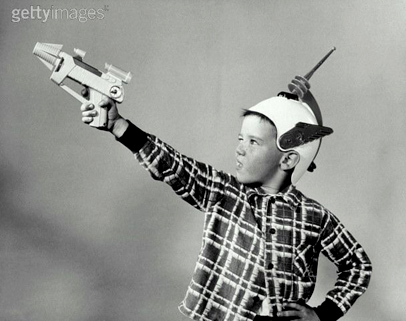
\includegraphics[width=2.0in]{Images/remco_gun_boy2.jpg}}
\item[\redcirc] \highpriority\ \redtext{Interface with Moray}
\pause
\item[$\bigcirc$] \ldots ?
\end{enumerate}
\end{minipage}
\end{center}
\end{frame}

 % What is needed to complete V6.0 (radiation)?
%======================================================================
\NEWSEC
%======================================================================

\subsection{\ssContribute}

\begin{frame}[fragile,label=ss-contribute] 
\label{frame:help}
\secframetitle{\ssContribute}
\textbf{Thanks for asking!} \\ \ \\
\begin{minipage}{4.5in}
\begin{center}
\rowcolors[]{1}{blue!5}{blue!10}
\begin{tabular}{rl}
\uncover<1->{\orow{\textbf{Beta User}}} &
  \uncover<1->{\orow{download and experiment with \enzop}} \\
  \uncover<2->{\orow{\textbf{Testing}}} &
  \uncover<2->{\orow{develop and submit test problems}} \\
  \uncover<3->{\erow{\textbf{Debugging}}} &
  \uncover<3->{\erow{help track down and fix bugs}} \\
  \uncover<4->{\orow{\textbf{Documentation}}} &
  \uncover<4->{\orow{write or update documentation}} \\
  \uncover<5->{\erow{\textbf{Developing}}} &
  \uncover<5->{\erow{migrate \enzo\ physics capabilities to \enzop }} \\
  \uncover<6->{\erow{\textbf{Refactoring}}} &
  \uncover<6->{\erow{refactor uglier or more complicated code sections}} \\
  \uncover<7->{\orow{\textbf{Managing}}} &
  \uncover<7->{\orow{help direct the development effort}}
 \end{tabular}
\end{center}
\end{minipage} \\

\end{frame}
 % How can I contribute?
%======================================================================
\NEWSEC
%======================================================================

\subsection{\ssFutureSummary}

%----------------------------------------------------------------------

\begin{frame}[fragile,label=ss-future-summary] 
\secframetitle{\ssFutureSummary}
\begin{itemize}
\item Enzo-P / Cello development entering a new stage
\begin{itemize}
\item pipelined development
\item Enzo-P: new physics capabilities
\item Cello: new framework support
\end{itemize}
\item Requires multiple developers!
\begin{itemize}
\item Dan Reynolds working on scalable gravity
\item More help wanted!
\end{itemize}
\end{itemize}
\vfill
\centerline{$\qed$}
\end{frame}



  %======================================================================
\NEWMOD
%======================================================================

\section{\sProject}

%----------------------------------------------------------------------

\logo{\hfill\hyperlink{outline<1>}{\icon}}

\begin{frame}[fragile,label=s-project] 
\modframetitle{\sProject}
\small
\begin{center}
\begin{minipage}{3.25in}
\begin{enumerate}
\item \hyperlink{ss-project<1>}       {\BUTTON {\orow{\ssProject}}} \\
\item \hyperlink{ss-source<1>}        {\BUTTON {\erow{\ssSource}}} \\
%\item \hyperlink{ss-browse<1>}        {\BUTTON {\orow{\ssBrowse}}} \\
\item \hyperlink{ss-documentation<1>} {\BUTTON {\erow{\ssDocumentation}}} \\
\item \hyperlink{ss-testing<1>}       {\BUTTON {\orow{\ssTesting}}} \\
\item \hyperlink{ss-bugs<1>}          {\BUTTON {\erow{\ssBugs}}} \\
\item \hyperlink{ss-project-summary<1>} {\BUTTON {\erow{\ssProjectSummary}}} \\
%\hyperlink{ss-communicate<1>}   {\BUTTON {\orow{\ssCommunicate}}}
\end{enumerate}
\end{minipage}
\end{center}
\end{frame}

\logo{\hfill\hyperlink{s-project<1>}{\icon}}

%======================================================================
\NEWSEC
%======================================================================

\subsection{\ssProject}

\begin{frame}[fragile,label=ss-project] 
\secframetitle{\ssProject}
\blockblue
\vspace{-0.2in}
\begin{center}
\begin{minipage}{3.5in}
\rowcolors[]{1}{blue!5}{blue!10}
\begin{tabbing}
xxxxx\=xxxxxxxxxxxxxxxxx\= \kill
\rule{\textwidth}{0.1mm} \\[-0.1cm]
\bluetext{\textbf{Project website}} \\[-0.1cm]
 \> \greentext{\url{http://cello-project.org}} \\[-0.2cm]
\rule{\textwidth}{0.1mm} \\[-0.1cm]
\bluetext{{Source code}} \> \> \redtext{\code{cello-src/src}} \\[-0.1cm]
 \> \greentext{\url{https://bitbucket.org/cello-project}} \\[-0.2cm]
\rule{\textwidth}{0.1mm} \\[-0.1cm]
\bluetext{{Documentation}} \>  \> \redtext{\code{cello-doc/source}} \\[-0.1cm]
 \> \greentext{\url{http://cello-project.org/doc}} \\[-0.2cm]
\rule{\textwidth}{0.1mm} \\[-0.1cm]
\bluetext{{Test suite}}  \> \> \redtext{\code{cello-src/test}} \\[-0.1cm]
 \> \greentext{\url{http://cello-project.org/test}} \\[-0.2cm]
\rule{\textwidth}{0.1mm} \\[-0.1cm]
\bluetext{{Bug tracking}} \> \> \redtext{\code{cello-bug}} \\[-0.1cm]
 \> \greentext{\url{http://cello-project.org/bug}}  \\[-0.2cm]
\rule{\textwidth}{0.1mm} \\[-0.1cm]
\bluetext{{Mailing List}} \\[-0.1cm]
 \> \greentext{\footnotesize{\url{https://mailman.ucsd.edu/mailman/listinfo/cello-l/}}}
\end{tabbing}
\end{minipage}
\end{center}

\end{frame}
%----------------------------------------------------------------------
 % How is the Enzo-P project currently organized?
%======================================================================
\NEWSEC
%======================================================================

\subsection{\ssSource}

\begin{frame}[fragile,label=ss-source] 
\secframetitle{\ssSource}
\begin{itemize}
\item \greentext{\url{https://bitbucket.org/cello-project}}
\item \bluetext{Current project members} \\
\footnotesize
Michael Norman \\
James Bordner \\ 
Tom Abel \\
Greg Bryan \\
Dave Collins \\ 
Alexei Kritsuk \\ 
Brian O'Shea \\
Daniel Reynolds \\ 
Matthew Turk \\ 
John Wise \\
\normalsize
\item \bluetext{Repository:} \redcode{cello-src} \\
\small{\orangecode{hg clone ssh://hg@bitbucket.org/cello-project/cello-src}}
\end{itemize}
\end{frame}

\begin{frame}[fragile] 
\secframetitle{\ssSource}
\begin{itemize}
\item \bluetext{Basic directory structure: \redcode{cello-src/}\ldots} \\
\begin{tabular}{ll}
\redcode{src/Enzo} & \bluetext{Enzo-P source} \\
\redcode{src/Cello} & \bluetext{Cello source} \\
\redcode{bin/enzo-p} & \bluetext{executable} \\
\redcode{input} & \bluetext{sample parameter files} \\
\redcode{test} & \bluetext{tests and results} \\
\redcode{tools} & \bluetext{convenience utilities}
\end{tabular}
\item \bluetext{Some useful files} \\
\begin{tabular}{ll}
\redcode{build.sh} & \bluetext{Build script} \\
\redcode{SContstruct} & \bluetext{Top-level ``make'' file}\\
\redcode{errors.org} & \bluetext{Generated \code{org-mode} errors / warnings} \\
\redcode{diff.org} & \bluetext{Generated \code{org-mode} \greencode{hg diff}} \\
\redcode{log.org} & \bluetext{Generated \code{org-mode} \greencode{hg log}}
\end{tabular}

\end{itemize}
\end{frame}

 % Where is the source code hosted?
%%======================================================================
\NEWSEC
%======================================================================

\subsection{\ssBrowse}

\begin{frame}[fragile,label=ss-browse] 
\secframetitle{\ssBrowse}
\begin{enumerate}
\item \bluetext{Bitbucket}
\begin{itemize}
\item \greentext{\url{https://bitbucket.org/cello-project/cello-src/src}}
\item \bluetext{good for viewing development history}
\end{itemize}
\item \bluetext{Doxygen on \code{cello-project.org} platform}
\begin{itemize}
\item \greentext{\url{http://cello-project.org/src}}
\item \bluetext{good for viewing annotated code structure}
\end{itemize}
\item \bluetext{Doxygen on your laptop}
\begin{itemize}
\item \redcode{make doc}
\item \greentext{\footnotesize\url{file:///home/bordner/Cello/cello-src/}\underline{src-html}\url{/index.html}}
\item \redcode{cd \underline{src-latex}; pdflatex refman.tex}
\end{itemize}
\end{enumerate}

\end{frame}

 % How can I browse the source code?
%======================================================================
\NEWSEC
%======================================================================

\subsection{\ssDocumentation}

\begin{frame}[fragile,label=ss-documentation] 
\secframetitle{\ssDocumentation}
\begin{itemize}
\item \greentext{\url{http://cello-project.org} / \framebox{Documentation}}
\begin{itemize}
\item \bluetext{Getting Started Using Enzo-P} \\
      \greentext{download; configure; port; build; run}
\item \bluebf{Enzo-P/Cello parameters reference} \\
      \greenbf{up-to-date list of \textit{all} Enzo-P/Cello parameters}
\item \bluetext{Parameter Files} \\
      \greentext{describes Cello's structured parameter files}
\item \bluetext{Parameter File Example} \\
      \greentext{explains the parameter file used in Getting Started}
\item \bluetext{Enzo-P / Cello Guiding Principles} \\
      \greentext{performance, scalability, usability, reliability, and flexibility}
\item \bluetext{Design} \\
      \greentext{Top-level component design of Cello}
\end{itemize}
\item Documentation is in a state of flux: .pdf $\rightarrow$ .rst
\end{itemize}
\end{frame}

 % What documentation is available?
%======================================================================
\NEWSEC
%======================================================================

\subsection{\ssTesting}

\begin{frame}[fragile,label=ss-testing] 
\secframetitle{\ssTesting}
\begin{itemize}
\item \greentext{\url{http://cello-project.org} / \framebox{Regression tests}}
\item \bluetext{Regression tests available in} \redcode{cello-src}
\item \redcode{\$ make test} \bluetext{(takes about 30-60 minutes)}
\item \bluetext{Tests parameter files in} \redcode{cello-src/input}
\item \bluetext{Tests are run in} \redcode{cello-src/test}
\item \bluetext{Test results viewable via}  \redcode{cello-src/test/index.php}
\end{itemize}
\end{frame}

\begin{frame}[fragile] 
\secframetitle{\ssTesting}
\framesubtitle{Enzo-P/Cello Test Results: header table}
\begin{minipage}{1.75in}
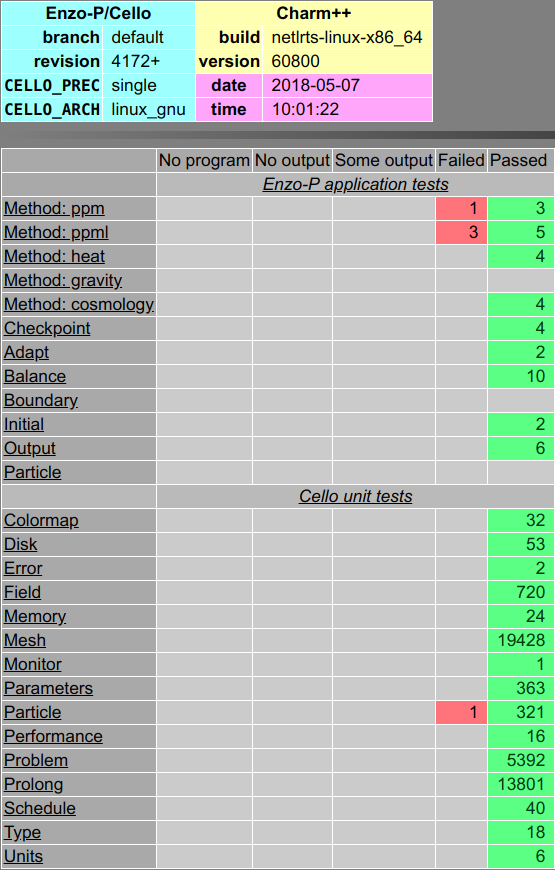
\includegraphics[width=1.75in]{Images/test-1.png}
\end{minipage} \ 
\begin{minipage}{2.25in}
\begin{itemize}
\item Summary of all tests
\item Columns:
\footnotesize
\begin{enumerate}
\item didn't compile
\item didn't start
\item didn't finish
\item tests failed
\item tests passed
\end{enumerate}
\small
\item A few failed tests are expected
\item Sections link to details
\end{itemize}
\end{minipage}
\end{frame}

%----------------------------------------------------------------------

\begin{frame}[fragile] 
\secframetitle{\ssTesting}
\framesubtitle{Enzo-P/Cello Test Results: adaptive mesh refinement}
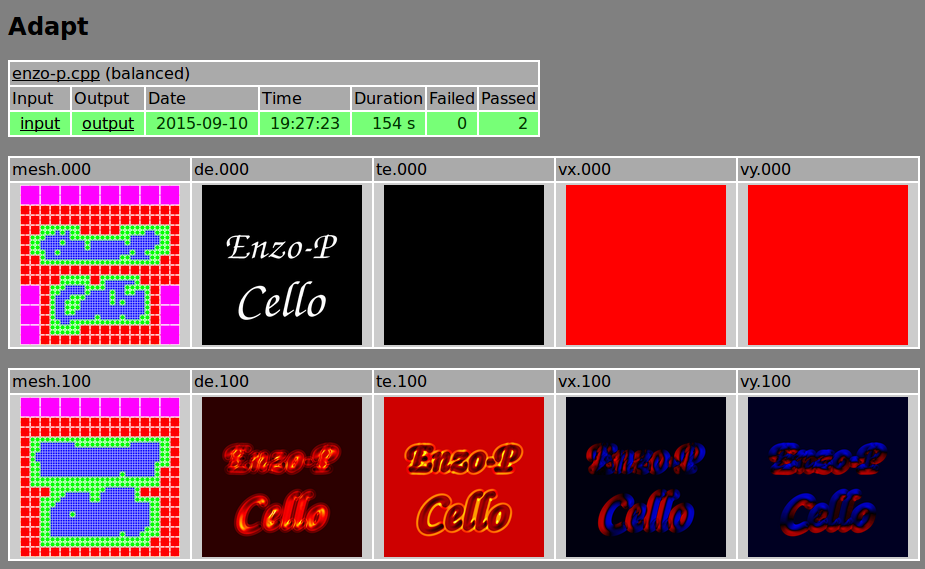
\includegraphics[width=4.0in]{Images/cello-test-2.png}
\end{frame}


\begin{frame}[fragile] 
\secframetitle{\ssTesting}
\framesubtitle{Enzo-P/Cello Test Results: dynamic load balancing}
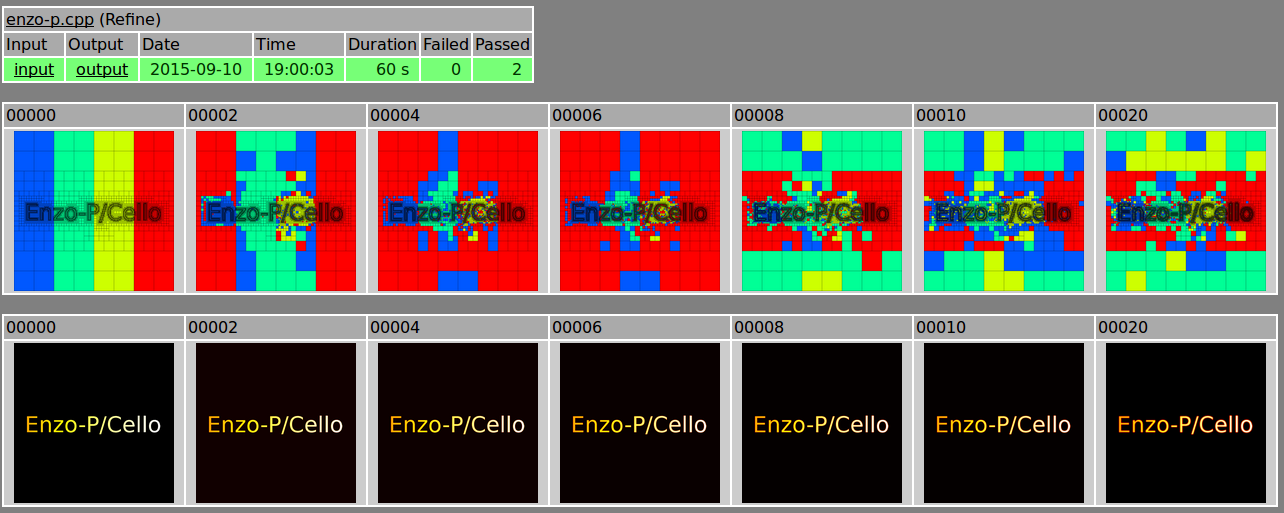
\includegraphics[width=4.0in]{Images/cello-test-3.png}
\end{frame}

 % How is testing done?
%======================================================================
\NEWSEC
%======================================================================

\subsection{\ssBugs}

\begin{frame}[fragile,label=ss-bugs] 
\secframetitle{\ssBugs}
\begin{itemize}
\item \greentext{\url{http://cello-project.org} / \framebox{Bug tracking}}
\end{itemize}
\rowcolors[]{1}{blue!5}{blue!10}
\begin{center}
\vspace{-0.1in}
\begin{minipage}{4.5in}
\footnotesize
\begin{tabular}{rll}
% (As of 2015-09-03)
% 2	2013-06-18 	Excessive syncronization during mesh adaptation 
% 3	2013-06-18 	Multiple refresh steps are performed 
% 4	2013-06-18 	ProlongLinear requires ghost depth of four 
% 12	2013-09-10 	Parallel runs may crash in inteuler with numerical errors 
% 13	2014-08-19 	I/O is incorrect for ip stride != 1 
% 19	2015-03-26 	method_ppm-1 and method_ppm-8 produce slightly different results
% 21	2014-03-17 	Small errors near corners of just-refined blocks 
% 31	2014-01-22 	Refresh errors in larger-scale parallel runs 
% 34	2014-02-21 	Several components seem to have memory leaks 
% 36	2014-03-17 	Adapt crashes (surprise) in sdsc-demo.in 
% 40	2014-04-29 	adapt-L5 problem fails sometimes 
% 45	2014-05-11 	Performance output for components seems incorrect 
% 46	2015-05-06 	Adapt seems to not be coarsening some blocks that should coarsen 
% 51	2014-06-27 	Parameter file syntax error messages display incorrect line number 
% 56	2014-08-21 	Restart fails when number of processors is changed 
% 57	2014-09-25 	stale Charm++ array messages in double mach problem cycle 846 
% 59	2014-11-20 	Occasional segmentation faults in file output from dereferencing null file_ pointer 
% 60	2015-07-06 	Load balancing unit tests occasionally hang 
% 68	2015-03-10 	Gravity solver still diverges sometimes 
% 72	2015-05-08 	RefineSlope does not work correctly sometimes 
% 73	2015-06-12 	New implementation of Refresh sometimes hangs sometimes crashes 
% 74	2015-06-16 	Enzo-P crashes in parse.l with Charm version 6.6.1 with P > 1 
% 75	2015-06-18 	method_heat-8 regression test failed 
% 76	2015-07-07 	Refresh add_fields() does not work as expected 
% 78	2015-07-15 	Mg0 solver has grid-effects 
% 79  	2015-07-27      Synchronization in Refresh is incorrect for Mg0
\uncover<1->{ID} & Date & \centerline{\uncover<1->{Summary}} \\
\hline
{\erow{151}} &	2018-05-03 &\erow{Single root block Cosmo crashes in refinement} \\
{\orow{150}} &	2018-04-26 &\orow{Memory leak in Cosmology problems} \\
{\erow{148}} &	2018-04-17 &\erow{load balancing fails when Index bit ordering is changed} \\
{\orow{147}} &	2018-04-17 &\orow{Errors with netlrs smp charm++} \\
{\erow{146}} &	2018-04-02 &\erow{Restart fails for Cosmo\_OsNa problem on SDSC Comet} \\
{\orow{138}} &	2018-02-07 &\orow{Image output fails with ``image\_ already created''} \\
{\erow{126}} &	2017-08-31 &\erow{data output of particles generates corrupt HDF5 files} \\
{\orow{118}} &	2017-07-12 &\orow{HDF5 output does not scale on Blue Waters} \\
{\erow{111}} & 	2017-06-08 &\erow{Adapt fails if octree array axis is not power of 2}
\end{tabular}
\end{minipage}
\end{center}
\end{frame}

 % What are some of the known bugs?
%======================================================================
\NEWSEC
%======================================================================

\subsection{\ssProjectSummary}

%----------------------------------------------------------------------

\begin{frame}[fragile,label=ss-project-summary] 
\secframetitle{\ssProjectSummary}
\begin{itemize}
\item The Enzo-P / Cello project is comprised of multiple components
\item Project page: \url{http://cello-project.org}
\item Source code
\begin{itemize}
\item  \code{http://bitbucket.org/cello-project}
\end{itemize}
\item Documentation
\begin{itemize}
\item doxygen auto-generated:  \code{cello-src/src-html}
\item restructured-text: \code{cello-doc/source}
\end{itemize}
\item Regression testing
\begin{itemize}
\item  \code{cello-src/test}
\item easy to run: \code{make test}
\item results easy to view: \code{cello-src/test/index.php}
\end{itemize}
\item Bug tracking and debugging
\begin{itemize}
\item Bugzilla: \url{http://cello-project.org/bug}
\item Debugging scripts: \code{cello-bug}
\end{itemize}
\end{itemize}
\vfill
\centerline{$\qed$}
\end{frame}

 
%%======================================================================
\NEWSEC
%======================================================================

\subsection{\ssCommunicate}

\begin{frame}[fragile,label=ss-communicate] 
\secframetitle{\ssCommunicate}
\end{frame}

 % How do Enzo-P developers communicate?

  %======================================================================
\NEWMOD
%======================================================================

\section{\sStarting}

%----------------------------------------------------------------------

\logo{\hfill\hyperlink{outline<1>}{\icon}}

\begin{frame}[fragile,label=s-starting] 
\modframetitle{\sStarting}
\small
\begin{center}
\begin{minipage}{3.25in}
\begin{enumerate}
\item \hyperlink{ss-starting<1>}      {\BUTTON {\ssStarting}}
\item \hyperlink{ss-install-charm<1>} {\BUTTON {\ssInstallCharm}}
\item \hyperlink{ss-install-enzop<1>} {\BUTTON {\ssInstallEnzop}}
\item \hyperlink{ss-configure<1>}     {\BUTTON {\ssConfigure}}
\item \hyperlink{ss-compile<1>}       {\BUTTON {\ssCompile}}
\item \hyperlink{ss-running<1>}       {\BUTTON {\ssRunning}}
%\item \hyperlink{ss-doublemach<1>}    {\BUTTON {\ssDoubleMach}}
%\item \hyperlink{ss-restart<1>}       {\BUTTON {\ssRestart}}
%\item \hyperlink{ss-load-balance<1>}  {\BUTTON {\ssLoadBalance}}
%\item \hyperlink{ss-tools<1>}         {\BUTTON {\ssTools}}
%\item \hyperlink{ss-starting-summary<1>} {\BUTTON {\ssStartingSummary}}
\end{enumerate}
\end{minipage}
\end{center}
\end{frame}

\logo{\hfill\hyperlink{s-starting<1>}{\icon}}

%======================================================================
\NEWSEC
%======================================================================

\subsection{\ssStarting}

\begin{frame}[fragile,label=ss-starting] 
\secframetitle{\ssStarting}

Enzo-P requires several steps to download and compile

\begin{enumerate}
\item \bluetext{download and install Charm++}
\item \bluetext{download and install dependent libraries} (\redcode{hdf5, libpng} (\redcode{csh},\redcode{bc}))
\item \bluetext{download Enzo-P / Cello}
\item \bluetext{configure and compile \code{bin/enzo-p}}
\item \bluetext{run a test problem}
\end{enumerate}

\pause
\ \\
\ \\
\centerline{\redbf{Let's install and run Enzo-P!}}

\end{frame}

 % Geting started using Enzo-P / Cello
%======================================================================
\NEWSEC
%======================================================================

\subsection{\ssInstallCharm}


\begin{frame}[fragile,label=ss-install-charm] 
\secframetitle{\ssInstallCharm}
\framesubtitle{Charm++ website: \urltext{http://charm.cs.illinois.edu}}
You will likely have to download and install Charm++ yourself
\begin{center}
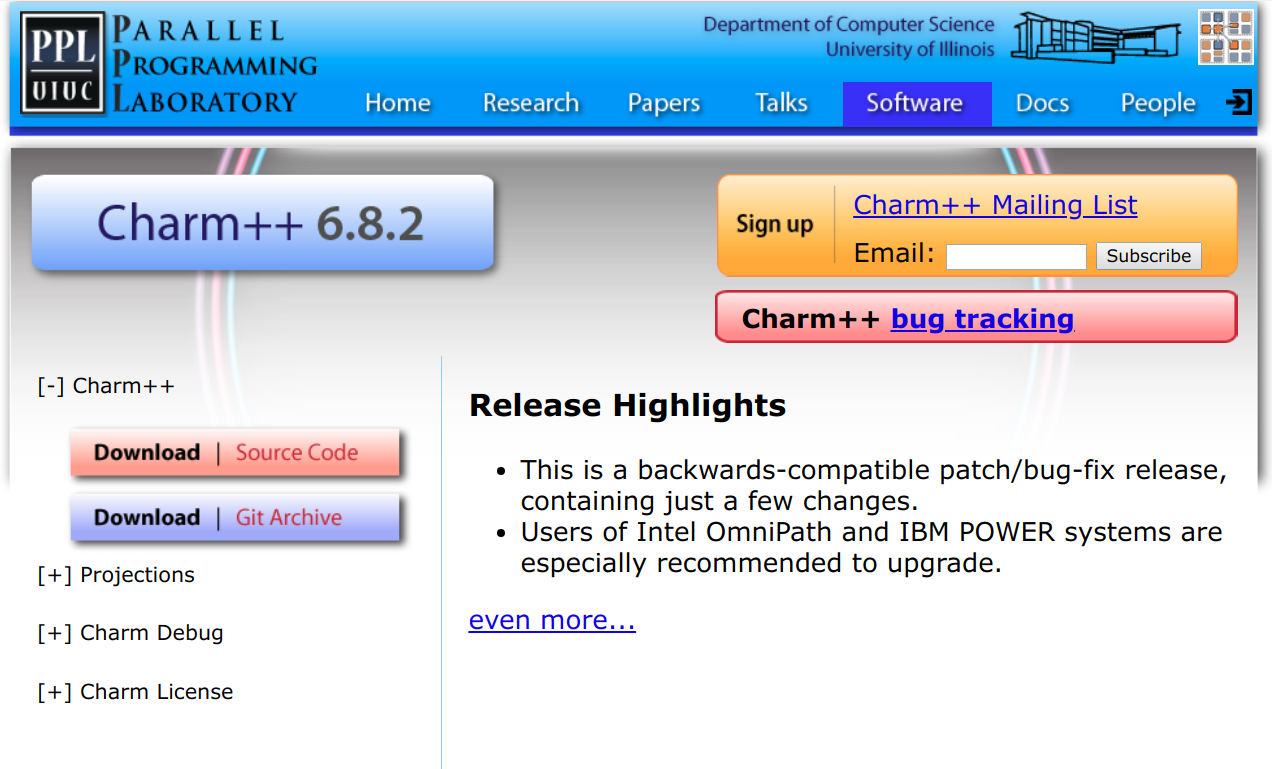
\includegraphics[width=4.00in]{charm-download.png}
\end{center}
\end{frame}


\setbeamercolor{block title}{bg=blue!30,fg=black}

%\usebackgroundtemplate
%{\includegraphics[width=5in]{monitor-2.png}}

\setbeamercolor{monitor-2.png}{bg=RGB{43,43,51}}

%----------------------------------------------------------------------

\begin{frame}[fragile] 
\secframetitle{\ssInstallCharm}
\color{black}
\footnotesize
%\begin{center}
%\begin{minipage}{3.3in}
%\begin{block}<+->{\textbf{Install \charm}}
\prompt             \redcode{ mkdir \url{~}/Charm}\cursor{1}  \\
\uncover<2->{\prompt\redcode{ cd \url{~}/Charm}\cursor{2}}  \\
\uncover<3->{\prompt\redcode{ wget http://charm.cs.illinois.edu/distrib/charm-6.8.2.tar.gz}\cursor{3}}  \\
\uncover<3->{\prompt\redcode{ (wget http://client64-249.sdsc.edu/\url{~}bordner/charm-6.8.2.tar.gz}\cursor{3})}  \\
\uncover<4->{\prompt\redcode{ tar zxf charm-6.8.2.tar.gz}\cursor{4}}  \\
\uncover<5->{\prompt\redcode{ ln -s charm-6.8.2 charm}\cursor{5}}  \\
\uncover<6->{\prompt\redcode{ cd charm}\cursor{6}}  \\
\uncover<7->{\blueit{   \#  build directly (recommended for Mac's)}} \\
\uncover<7->{\prompt\redcode{ ./build charm++ netlrts-darwin-x86\_64 gcc gfortran -j4 \textendash\textendash with-production}\cursor{7}} \\
\uncover<8->{\blueit{   \# \redbf{\textbf{or}} build directly (recommended for Linux)}} \\
\uncover<8->{\prompt\redcode{ ./build charm++ netlrts-linux-x86\_64   -j4  \textendash\textendash with-production}\cursor{8}} \\
\uncover<9->{\blueit{   \# \redbf{\textbf{or}} run the interactive build script:}} \\
\uncover<9->{\prompt\redcode{ ./smart-build.pl}\cursor{9}} \\
%\end{block}
%\end{minipage}
%\end{center}
\end{frame}


%----------------------------------------------------------------------

\begin{frame}[fragile] 
\secframetitle{\ssInstallCharm}
\framesubtitle{Compiling \charm\ with \code{./smart-build.pl}}
\color{black}
\footnotesize

\prompt\redcode{./smart-build.pl}\cursor{1}
\pause

\verb@============================================================@ \\
\ \\
\verb@Begin interactive charm configuration ...@\\
\verb@If you are a poweruser expecting a list of options, please use@ \\
\verb@   ./build --help@\\
\ \\
\verb@============================================================@ \\
\ \\
\verb@Are you building to run just on the local machine, and not across@ \\
\verb@multiple nodes? [y/N]@\cursor{2} \\
\pause
\verb@I found that you have an mpicc available in your path.@ \\
\verb@Do you want to build Charm++ on this MPI? [y/N]:@\cursor{3} \\
\end{frame}

%----------------------------------------------------------------------

\begin{frame}[fragile] 
\secframetitle{\ssInstallCharm}
\framesubtitle{Compiling \charm\ with \code{./smart-build.pl}}
\color{black}
\footnotesize

\verb@Do you have a special network interconnect? [y/N]:@\cursor{1}
\pause
\verb@y@ \\
\verb@	Choose an interconnect from below: [1-10]@ \\
\verb@		 1) MPI@ \\
\verb@		 2) Infiniband (ibverbs)@ \\
\verb@		 3) Cray XE, XK@ \\
\verb@		 4) Cray XC@ \\
\verb@		 5) Blue Gene/Q@ \\
\verb@		 6) Intel Omni-Path (ofi)@ \\
\verb@  @\cursor{2}
\end{frame}

%----------------------------------------------------------------------

\begin{frame}[fragile] 
\secframetitle{\ssInstallCharm}
\framesubtitle{Compiling \charm\ with \code{./smart-build.pl}}
\color{black}
\footnotesize

\verb@How do you want to handle SMP/Multicore: [1-3]@ \\
\verb@      1) single-threaded [default]@ \\
\verb@      2) SMP@ \\
\verb@      3) POSIX Shared Memory@ \\
\verb@  @\cursor{1}
\pause
\ \\
\verb@Do you want to specify a compiler? [y/N]@\cursor{2}\pause\verb@n@ \\
\ \\
\verb@Do you want to specify any Charm++ build options, such as fortran@ \\
\verb@   compilers? [y/N]@\cursor{3} \\

\end{frame}

%----------------------------------------------------------------------

\begin{frame}[fragile] 
\secframetitle{\ssInstallCharm}
\framesubtitle{Compiling \charm\ with \code{./smart-build.pl}}
\color{black}
\footnotesize

\verb@Choose a set of compiler flags [1-5]@ \\
\verb@	1) none@ \\
\verb@	2) debug mode                      -g -O0@ \\
\verb@	3) production build [default]      --with-production@ \\
\verb@	4) production build w/ projections --with-production --enable-tracing@ \\
\verb@	5) custom@ \\
\verb@  @\cursor{1}
\pause
\ \\ \ \\
\verb@What do you want to build?@ \\
\verb@          1) Charm++ [default] (choose this if you are building NAMD)@ \\
\verb@          2) Charm++ and AMPI@ \\
\verb@          3) Charm++, AMPI, ParFUM, FEM and other libraries@ \\
\verb@  @\cursor{2}
\end{frame}

%----------------------------------------------------------------------

\begin{frame}[fragile] 
\secframetitle{\ssInstallCharm}
\framesubtitle{Compiling \charm\ with \code{./smart-build.pl}}
\color{black}
\footnotesize
\ \\
\verb@Do you want to compile in parallel?@ \\
\verb@        1) No@ \\
\verb@        2) Build with -j2@ \\
\verb@        3) Build with -j4@ \\
\verb@        4) Build with -j8 @ \\
\verb@        5) Build with -j16 [default]@ \\
\verb@        6) Build with -j32@ \\
\verb@        7) Build with -j@ \\
\verb@  @\cursor{1}
\ \\
\pause
\verb@We have determined a suitable build line is:@ \\
\verb@	./build charm++ net-linux-x86_64  -j4  --with-production@ \\
\ \\
\verb@Do you want to start the build now? [Y/n]@\cursor{2} \pause\code{y}\\
\verb@Building with: ./build charm++ net-linux-x86_64  -j4 --with-production@

\end{frame}


%----------------------------------------------------------------------

% \begin{frame}[fragile] 
% \secframetitle{\ssInstallCharm}
% \framesubtitle{Running a \charm\ test problem}
% \color{black}
% \footnotesize
% 
% \prompt\redcode{ cd examples/charm++/hello/1darray}\cursor{1}\\\pause
% \prompt\redcode{ make test}\cursor{2}\\\pause
% 
% \color{blue}
% \verb@ ./charmrun +p4 hello 10@ \\
% \color{black}
% \verb@	Charmrun> started all node programs in 1.296 seconds. @ \\
% \verb@	Converse/Charm++ Commit ID:  @ \\
% \verb@	Trace: traceroot: /home/bordner/Charm/682/gnu/net/charm-6.8.2/examples/charm++/hello/1darray/hello @ \\
% \verb@	Charm++> scheduler running in netpoll mode. @ \\
% \verb@	CharmLB> Load balancer assumes all CPUs are same. @ \\
% \verb@	Charm++> Running on 1 unique compute nodes (8-way SMP). @ \\
% \verb@	Charm++> cpu topology info is gathered in 0.001 seconds. @ \\
% \verb@	Running Hello on 4 processors for 10 elements @ \\
% \verb@	Hello 0 created @ \\
% \verb@	Hello 1 created @ \\
% \verb@	Hello 2 created @ \\
% \verb@	Hi[17] from element 0 @ \\
% \verb@	Hi[18] from element 1 @ \\
% \verb@	Hi[19] from element 2 @ \\
% \verb@	Hello 6 created @ \ldots
% \end{frame}

\usebackgroundtemplate
{}

 % How do I download and install Charm++?
%======================================================================
\NEWSEC
%======================================================================

\subsection{\ssInstallEnzop}

%----------------------------------------------------------------------
\begin{frame}[fragile,label=ss-install-enzop] 
\secframetitle{\ssInstallEnzop}
\framesubtitle{Enzo-P source code: \url{https://bitbucket.org/cello-project}}
\footnotesize \enzopcello\ source is available from \textcolor{green!50!black}{\url{https://bitbucket.org/cello-project}}
\begin{center}
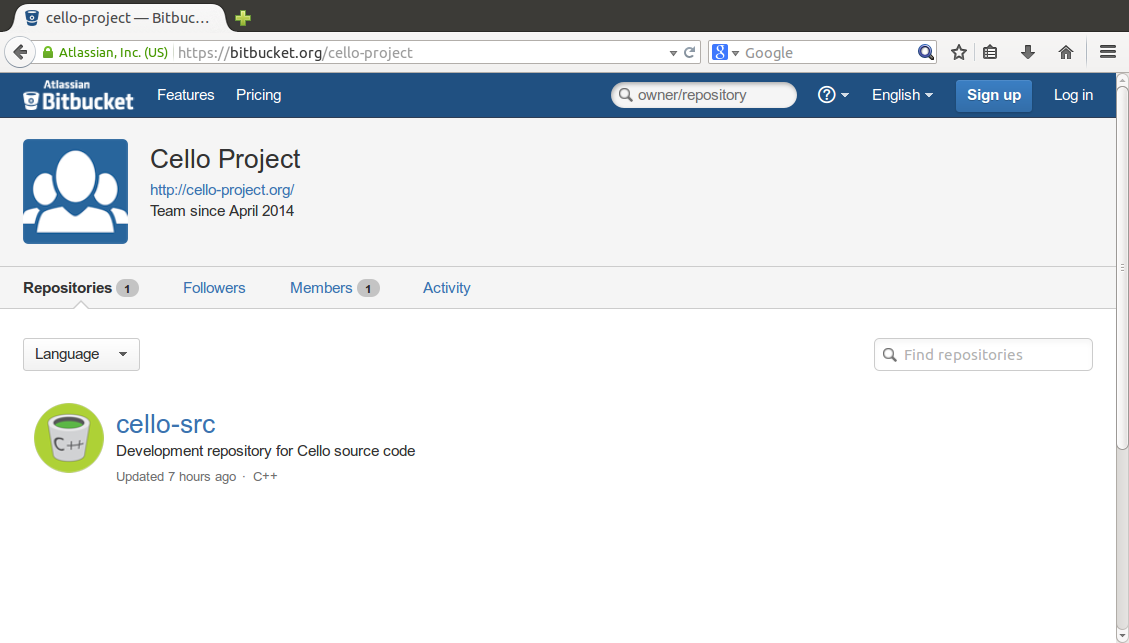
\includegraphics[width=4.00in]{cello-download.png}
\end{center}
\end{frame}
\setbeamercolor{monitor-2.png}{bg=RGB{43,43,51}}

%----------------------------------------------------------------------
\begin{frame}[fragile] 
\secframetitle{\ssInstallEnzop}
\framesubtitle{Downloading Enzo-P/Cello}
\footnotesize
\begin{semiverbatim}
 \prompt\ \redcode{hg clone https://bitbucket.org/cello-project/cello-src}\cursor{1}  
 \uncover<2->{destination directory: cello-src}
 \uncover<2->{requesting all changes}
 \uncover<2->{adding changesets} 
 \uncover<2->{adding manifests} 
 \uncover<2->{adding file changes} 
 \uncover<2->{added 3529 changesets with 21657 changes to 4353 files (+1 heads)} 
 \uncover<2->{updating to branch default} 
 \uncover<2->{resolving manifests} 
 \uncover<2->{\vdots}
 \uncover<2->{getting scons-LICENSE}
 \uncover<2->{getting scons-README}
 \uncover<2->{getting scons-local-2.2.0/SCons/Action.py}
 \uncover<2->{924 files updated, 0 files merged, 0 files removed, 0 files unresolved}
\end{semiverbatim}
\end{frame}

 % How do I download and install Enzo-P?
%======================================================================
\NEWSEC
%======================================================================

\subsection{\ssConfigure}


%    SConstruct
%    config/linux_blah

%    CELLO_PREC
%    CELLO_ARCH
%    (move prec to config?)
%   use online user documentation
%----------------------------------------------------------------------

\begin{frame}[fragile,label=ss-configure] 
\secframetitle{\ssConfigure}
%\framesubtitle{Configuring Enzo-P/Cello: \code{config/*.py}}
\footnotesize
\begin{enumerate}
\item Use or create a small config/*.py machine file
\item Set CELLO environment variables
\item Edit SConstruct user-configuration section (optional)
\end{enumerate}
\begin{semiverbatim}
 \uncover<1->{\prompt \redcode{cd cello-src}}\cursor{1}  
 \uncover<2->{\prompt \redcode{ls config}}\cursor{2} 
 \uncover<3->{\greencode{davros_gnu_debug.py   gordon_gnu.py    linux_gprof.py   ncsa_bw.py}}
 \uncover<3->{\greencode{davros_gnu.py         gordon_intel.py  linux_mpe.py}}
 \uncover<3->{\greencode{faraday_gnu_debug.py  gordon_pgi.py    mf_gnu_debug.py}}
 \uncover<3->{\greencode{faraday_gnu.py        linux_gnu.py     mf_gnu.py}}
 \uncover<4->{\prompt \redcode{export CELLO_ARCH=linux_gnu}}\cursor{4}  
 \uncover<5->{\prompt \redcode{export CELLO_PREC=single}}\cursor{5}  
 \uncover<6->{\prompt \redcode{cat config/linux_gnu.py}}\cursor{6}  
\end{semiverbatim}
\end{frame}

%----------------------------------------------------------------------
\begin{frame}[fragile] 
\secframetitle{\ssConfigure}
\framesubtitle{Configuring Enzo-P/Cello: \code{config/*.py}}
\tiny
\begin{semiverbatim}
 \uncover<1->{\prompt \redcode{cat config/linux_gnu.py}}\cursor{1}  
 \uncover<2->{import os}
 \uncover<2->{}
 \uncover<2->{is_arch_valid = 1}
 \uncover<2->{}
 \uncover<2->{flags_arch = '-Wall -O3 -g'}
 \uncover<2->{flags_link_charm = ' -rdynamic' # required for backtraces}
 \uncover<2->{}
 \uncover<2->{cc  = 'gcc '}
 \uncover<2->{f90 = 'gfortran'}
 \uncover<2->{}
 \uncover<2->{flags_prec_single = ''}
 \uncover<2->{flags_prec_double = '-fdefault-real-8 -fdefault-double-8'}
 \uncover<2->{}
 \uncover<2->{libpath_fortran = '.'}
 \uncover<2->{libs_fortran    = ['gfortran']}
 \uncover<2->{}
 \uncover<2->{use_papi=1}
 \uncover<2->{papi_inc = '/usr/local/include'}
 \uncover<2->{papi_lib = '/usr/local/lib'}
 \uncover<2->{hdf5_inc     = '/usr/include'}
 \uncover<2->{hdf5_lib     = '/usr/lib'}
 \uncover<2->{png_path     = '/lib/x86_64-linux-gnu'}
 \uncover<2->{}
 \uncover<2->{home = os.environ['HOME']}
 \uncover<2->{charm_path   = home + '/Charm/charm'}
 \uncover<2->{grackle_path = home + '/Software/Grackle/src/clib'}
\end{semiverbatim}
\end{frame}

%----------------------------------------------------------------------
\begin{frame}[fragile] 
\secframetitle{\ssConfigure}
\framesubtitle{Configuring Enzo-P/Cello: \code{SConstruct}}
\tiny
\begin{semiverbatim}
\uncover<1->{\prompt \redcode{gedit SConstruct}}\cursor{1}  

#======================================================================
# USER CONFIGURATION
#======================================================================

#----------------------------------------------------------------------
# Whether to print out detailed messages with the TRACE() series of statements
#----------------------------------------------------------------------

trace = 0

#----------------------------------------------------------------------
# Whether to trace main phases
#----------------------------------------------------------------------

verbose = 0

#----------------------------------------------------------------------
# Whether to print out messages with the TRACE_CHARM() and TRACEPUP()
#  series of statements
#----------------------------------------------------------------------

trace_charm = 0

\end{semiverbatim}
\end{frame}

%----------------------------------------------------------------------
\begin{frame}[fragile] 
\secframetitle{\ssConfigure}
\framesubtitle{Configuring Enzo-P/Cello: \code{SConstruct}}
\tiny
\begin{semiverbatim}
\uncover<1->{\prompt \redcode{gedit SConstruct}}\cursor{1}  

#----------------------------------------------------------------------
# Whether to enable displaying messages with the DEBUG() series of
# statements. Also writes messages to out.debug.<P> where P is the
# (physical) process rank. Still requires the "DEBUG" group to be
# enabled in Monitor (that is Monitor::is_active("DEBUG") must be true
# for any output)
#----------------------------------------------------------------------

debug = 0

#----------------------------------------------------------------------
# Whether to periodically print all field values.  See
# src/Field/field_FieldBlock.cpp
#----------------------------------------------------------------------

debug_verbose = 0

\end{semiverbatim}
\end{frame}

%----------------------------------------------------------------------
\begin{frame}[fragile] 
\secframetitle{\ssConfigure}
\framesubtitle{Configuring Enzo-P/Cello: \code{SConstruct}}
\tiny
\begin{semiverbatim}
\uncover<1->{\prompt \redcode{gedit SConstruct}}\cursor{1}  

#----------------------------------------------------------------------
# Whether to track dynamic memory statistics.  Can be useful, but can
# cause problems on some systems that also override new [] () / delete
# [] ()
#----------------------------------------------------------------------

memory = 1

#----------------------------------------------------------------------
# Enable charm++ dynamic load balancing
#----------------------------------------------------------------------

balance = 1

\end{semiverbatim}
\end{frame}

%----------------------------------------------------------------------
\begin{frame}[fragile] 
\secframetitle{\ssConfigure}
\framesubtitle{Configuring Enzo-P/Cello: \code{SConstruct}}
\tiny
\begin{semiverbatim}
\uncover<1->{\prompt \redcode{gedit SConstruct}}\cursor{1}  
#----------------------------------------------------------------------
# Whether to compile with -pg to use gprof for performance profiling
#----------------------------------------------------------------------

use_gprof = 0

#----------------------------------------------------------------------
# Whether to compile with the Grackle chemistry and cooling library
#
# WARNING: must update grackle-related lines in src/Enzo/enzo.ci
#----------------------------------------------------------------------

use_grackle = 0

#----------------------------------------------------------------------
# Whether to run the test programs using valgrind to check for memory leaks
#----------------------------------------------------------------------

use_valgrind = 0

\end{semiverbatim}
\end{frame}

%----------------------------------------------------------------------
\begin{frame}[fragile] 
\secframetitle{\ssConfigure}
\framesubtitle{Configuring Enzo-P/Cello: \code{SConstruct}}
\tiny
\begin{semiverbatim}
\uncover<1->{\prompt \redcode{gedit SConstruct}}\cursor{1}  
#----------------------------------------------------------------------
# Whether to use Cello Performance class for collecting performance
# data (currently requires global reductions, and may not be fully
# functional) (basic time data on root processor is still output)
#----------------------------------------------------------------------

use_performance = 0

#----------------------------------------------------------------------
# Whether to compile the CHARM++ version for use with the Projections
# performance tool.
#----------------------------------------------------------------------

use_projections = 0

#----------------------------------------------------------------------
# How many processors to run parallel unit tests
#----------------------------------------------------------------------

ip_charm = '4'

#----------------------------------------------------------------------
# Whether this is a Mercurial repository
#----------------------------------------------------------------------

have_mercurial = 1
\end{semiverbatim}
\end{frame}

 % How do I configure Enzo-P?
%======================================================================
\NEWSEC
%======================================================================

\subsection{\ssCompile}

%----------------------------------------------------------------------
\begin{frame}[fragile,label=ss-compile] 
\secframetitle{\ssCompile}
\framesubtitle{Compiling Enzo-P/Cello}
\tiny
\begin{semiverbatim}
\uncover<1->{\prompt \redcode{make}}\cursor{1}  
\uncover<2->{./build.sh bin/enzo-p
Remove bin/enzo-p
2015-09-19 14:36:00 BEGIN
BEGIN Enzo-P/Cello ./build.sh
arch = linux_gnu
prec = double
target = bin/enzo-p
2015-09-19 14:36:00 compiling...                 PAPI installed

    CELLO_ARCH scons arch= linux_gnu
    CELLO_PREC scons prec= double

scons: warning: Two different environments were specified for target main_enzo.o,
	but they appear to have the same action: $CXX -o $TARGET -c $CXXFLAGS $CCFLAGS $_CCCOMCOM $SOURCES
File "/home/bordner/Cello/cello-src/build/Cello/SConscript", line 197, in <module>
/home/bordner/Charm/charm/bin/charmc -language charm++ -o build/Enzo/enzo-p.o -c -Wall -O3 -g -balancer Greed}
\uncover<3->{\vdots}
\uncover<4->{Install file: "build/Enzo/enzo-p" as "bin/enzo-p"
Success
done
END   Enzo-P/Cello ./build.sh: arch = linux_gnu  prec = double  target = bin/enzo-p time = 77s}
\uncover<5->{\prompt \redcode{charmrun +p4 bin/enzo-p input/test_implosion.in}}\cursor{5}
\end{semiverbatim}
\end{frame}

%----------------------------------------------------------------------
%\begin{frame}[fragile] 
% \secframetitle{\ssCompile}
%\framesubtitle{\url{https://bitbucket.org/cello-project/cello-src}}
%\footnotesize
%\begin{semiverbatim}
%% \uncover<1->{\prompt charmrun +p4 bin/enzo-p input/test_implosion.in}\cursor{9}

%\end{semiverbatim}
%\end{frame}

%   use online user documentation
%    generates
%       ./bin/enzo-p
%       ./errors.org

 % How do I compile Enzo-P?
%======================================================================
\NEWSEC
%======================================================================

\subsection{\ssRunning}

\begin{frame}[fragile,label=ss-running] 
\secframetitle{\ssRunning}
\framesubtitle{Enzo-P output: header text}
\tiny
\begin{semiverbatim}
\uncover<1->{\prompt \redcode{charmrun +p4 bin/enzo-p input/test_implosion.in}}\cursor{1}
\uncover<2->{Charmrun> started all node programs in 1.298 seconds.
Converse/Charm++ Commit ID: 
Charm++> scheduler running in netpoll mode.
CharmLB> Load balancer assumes all CPUs are same.
Charm++> Running on 1 unique compute nodes (8-way SMP).
Charm++> cpu topology info is gathered in 0.002 seconds.
UNIT TEST BEGIN
0 00001.06  ==============================================
0 00001.06  
0 00001.06    .oooooo.             oooo  oooo            
0 00001.06   d8P'  `Y8b            `888  `888            
0 00001.06  888           .ooooo.   888   888   .ooooo.  
0 00001.06  888          d88' `88b  888   888  d88' `88b 
0 00001.06  888          888ooo888  888   888  888   888 
0 00001.06  `88b    ooo  888    .o  888   888  888   888 
0 00001.06   `Y8bood8P'  `Y8bod8P' o888o o888o `Y8bod8P' 
0 00001.06  
0 00001.06  A Parallel Adaptive Mesh Refinement Framework
0 00001.06  
0 00001.06    Laboratory for Computational Astrophysics
0 00001.06          San Diego Supercomputer Center
0 00001.06       University of California, San Diego
0 00001.06  See 'LICENSE_CELLO' for software license information}
\end{semiverbatim}
\end{frame}
\begin{frame}[fragile]
\secframetitle{\ssRunning}
\framesubtitle{Enzo-P output: configuration settings}
\tiny
\begin{semiverbatim}
0 00001.06  BEGIN CELLO: Sep 19 14:37:45
0 00001.06 Define Simulation processors 4
0 00001.06 Define CELLO_ARCH linux_gnu
0 00001.06 Define CELLO_PREC double
0 00001.06 Define CC            gcc 
0 00001.06 Define CFLAGS        -Wall -O3 -g   
0 00001.06 Define CPPDEFINES    CONFIG_PRECISION_DOUBLE SMALL_INTS H5_USE_16_API NO_FREETYPE CONFIG_USE_PAPI 
PAPI3 CONFIG_USE_MEMORY CONFIG_HAVE_MERCURIAL CONFIG_USE_CHARM CONFIG_USE_CELLO
0 00001.06 Define CPPPATH       #/include /usr/local/include /usr/include
0 00001.06 Define CXX           /home/bordner/Charm/charm/bin/charmc -language charm++  
0 00001.06 Define CXXFLAGS      -Wall -O3 -g     -balancer GreedyCommLB -balancer GreedyLB -balancer HybridLB
 -balancer NeighborLB -balancer RandCentLB -balancer RefineCommLB -balancer RefineLB -balancer RotateLB
0 00001.06 Define FORTRANFLAGS  -Wall -O3 -g    -fdefault-real-8 -fdefault-double-8
0 00001.06 Define FORTRAN       gfortran
0 00001.06 Define FORTRANLIBS   gfortran
0 00001.06 Define FORTRANPATH   #/include
0 00001.06 Define LIBPATH       #/lib /usr/local/lib /usr/lib /lib/x86_64-linux-gnu/lib .
0 00001.06 Define LINKFLAGS     -Wall -O3 -g     -module GreedyCommLB -module GreedyLB -module HybridLB -modu
le NeighborLB -module RandCentLB -module RefineCommLB -module RefineLB -module RotateLB
0 00001.06 Define BUILD HOST    gedeckt
0 00001.06 Define BUILD DIR     /home/bordner/Cello/cello-src
0 00001.06 Define BUILD DATE    2015-09-19
0 00001.06 Define BUILD TIME    21:36:02
0 00001.06 Define CHARM_VERSION 60500
0 00001.06 Define CHANGESET     3841+
\end{semiverbatim}
\end{frame}
\begin{frame}[fragile]
\secframetitle{\ssRunning}
\framesubtitle{Enzo-P output: parameters accessed}
\tiny
\begin{semiverbatim}
0 00001.06  BEGIN ENZO-P
0 00001.06 Memory bytes 1013270 bytes_high 1013301
0 00001.06 Parameters read in input/test_implosion.in
0 00001.06 Parameters accessed Adapt:interval 1 [default]
0 00001.06 Parameters accessed Adapt:list[0] "SLOPE"
0 00001.06 Parameters accessed Adapt:SLOPE:type "slope"
0 00001.06 Parameters accessed Adapt:min_face_rank 0 [default]
0 00001.06 Parameters accessed Adapt:SLOPE:field_list[0] "density"
0 00001.06 Parameters accessed Adapt:SLOPE:min_refine 0.30000000000000 [default]
0 00001.06 Parameters accessed Adapt:SLOPE:max_coarsen 0.15000000000000 [default]
0 00001.06 Parameters accessed Adapt:SLOPE:max_level 2147483647 [default]
0 00001.06 Parameters accessed Adapt:SLOPE:level_exponent 0.0000000000000 [default]
0 00001.06 Parameters accessed Adapt:SLOPE:output  [default]
0 00001.06 Parameters accessed Adapt:SLOPE:include_ghosts false [default]
0 00001.06 Parameters accessed Boundary:type "reflecting"
0 00001.06 Parameters accessed Boundary:axis all [default]
0 00001.06 Parameters accessed Boundary:face all [default]
0 00001.06 Parameters accessed Domain:lower[0] 0.0000000000000
0 00001.06 Parameters accessed Domain:upper[0] 0.30000000000000
\vdots
\end{semiverbatim}
\end{frame}
\begin{frame}[fragile]
\secframetitle{\ssRunning}
\framesubtitle{Enzo-P output: simulation cycles}
\tiny
\begin{semiverbatim}
0 00002.07  -------------------------------------
0 00002.07 Simulation cycle 0000
0 00002.07 Simulation time-sim 0.000000000000e+00
0 00002.07 Simulation dt 0.000000000000e+00
0 00002.07 Performance unknown time-usec 0
0 00002.07 Performance simulation time-usec 3927213
0 00002.07 Performance cycle time-usec 0
0 00002.07 Performance cycle bytes-curr 0
0 00002.07 Performance cycle bytes-high 0
0 00002.07 Performance cycle bytes-highest 0
0 00002.07 Performance initial time-usec 971452
0 00002.07 Performance adapt time-usec 1326831
0 00002.07 Performance refresh time-usec 0
0 00002.07 Performance compute time-usec 0
0 00002.07 Performance output time-usec 1608215
0 00002.07 Performance stopping time-usec 0
0 00002.07 Performance simulation num-blocks 184
0 00002.07  -------------------------------------
\end{semiverbatim}
\end{frame}

%----------------------------------------------------------------------

\begin{frame}[fragile]
\secframetitle{\ssRunning}
\begin{minipage}{2.5in}
\only<1->{\ANIMATEGRAPHICS{width=2.5in}{20}{Images/Implosion/d-}{000}{200}}
\end{minipage}
%\begin{minipage}{2in}
%\only<2->{\ANIMATEGRAPHICS{width=2.0in}{20}{Images/Implosion/implosion-mesh-}{000}{200}}
%\end{minipage}
\end{frame}

 % How do I run an example problem?
%%======================================================================
\NEWSEC
%======================================================================

\subsection{\ssDoubleMach}

\begin{frame}[fragile,label=ss-doublemach] 
\secframetitle{\ssDoubleMach}
\framesubtitle{Test problem specification}

\footnotesize
\begin{center}

\includegraphics[width=4.0in]{Images/DoubleMachAmr/doublemach-de-0000.png}
\end{center}

\begin{tabbing}
xxxxxxxxxxxxxxxxxxxxxxxxxxxxxxxx\=xxxxxxxxxxxxxxxxxxx\=\kill
\> \bluetext{Adiabatic index}: \' $\gamma = 1.4$. \\
\> \bluetext{Grid domain}: \' $0.0 < x < 4.0$, $0.0 < y < 1.0$ \\
\> \bluetext{Shock}: \' Mach 10, $v_s$ = 10.0, \\
\> \bluetext{Angle}: \' 30 degrees. \\
\> \bluetext{Pre-shock conditions}: \' $P = 1.0$, $\rho = 1.4$, $v = 0.0$ \\
\> \bluetext{Post-shock conditions}: \' $P = 116.5$, $\rho = 8$, $v = 8.25$ \\
\> \bluetext{Time limit}: \' $t = 0.25$.
\end{tabbing}
\end{frame}

%----------------------------------------------------------------------

\begin{frame}[fragile] 
\secframetitle{\ssDoubleMach}
\framesubtitle{\group{Domain} and \group{Stopping} criteria}
\begin{itemize}
\item \group{Domain}

\begin{itemize}
\item $0.0 < x < 4.0, 0.0 < y < 1.0$
\begin{semiverbatim}
\group{Domain} \{ 
   \parameter{lower} = [\valuetext{0.0}, \valuetext{0.0}];
   \parameter{upper} = [\valuetext{4.0}, \valuetext{1.0}];
\} 
\end{semiverbatim}
\end{itemize}
%
\item \group{Stopping} criteria
\begin{itemize}
%
\item $t=0.25$
%
\begin{semiverbatim}
\group{Stopping} \{ \variable{time} = \valuetext{0.25}; \} 
\end{semiverbatim}
%
\end{itemize}
\end{itemize}
\end{frame}

%----------------------------------------------------------------------

 \begin{frame}[fragile] 
 \secframetitle{\ssDoubleMach}
 \framesubtitle{\group{Initial} conditions}
\footnotesize
Complex initial conditions can be specified directly.

 \begin{itemize}
 \item To specify $x = a(x,y,z)$ in subregion $A$, else $x = b(x,y,z)$:
 \begin{tabbing}
 xxxxxxx\=\kill
\parameter{x} = \code{[} \> \valuetext{a(x,y,z)} \comment{\# (floating-point expression)}, \\
\>                         \valuetext{A(x,y,z)} \comment{\# (logical expression)}, \\
\>                         \valuetext{b(x,y,z)} \comment{\# (floating-point expression)} ];
 \end{tabbing}
 \item E.g. to specify ``$\rho = 8$ if $x \le 1/6 + 0.57735 y$, else $\rho = 1.4$'':
\begin{semiverbatim}
\group{Initial} \{
    \subgroup{density} \{
        \parameter{value} = [\valuetext{8.0}, \valuetext{(x <= 0.16667 + 0.57735*y)}, 
                 \valuetext{1.4}];  \};
\}
\end{semiverbatim}
\item Repeat with \subgroup{velocity\_x}, \subgroup{velocity\_y}, \subgroup{total\_energy}
 \end{itemize}
\end{frame}

%----------------------------------------------------------------------

\begin{frame}[fragile] 
\secframetitle{\ssDoubleMach}
\framesubtitle{\group{Initial} conditions}
\footnotesize
\begin{itemize}
\item Repeat with \subgroup{velocity\_x}, \subgroup{velocity\_y}, and \subgroup{total\_energy}
\begin{semiverbatim}
\group{Initial} \{
    \subgroup{velocity_x} \{
       \parameter{value} = [ \valuetext{8.25*0.8660253},
                        \valuetext{(x <= 0.16667 + 0.57735*y)},
                 \valuetext{0.0} ]; \};
    \subgroup{velocity_y} \{
       \parameter{value} = [\valuetext{-8.25*0.5},
                        \valuetext{(x <= 0.16667 + 0.57735*y)},
                 \valuetext{0.0}]; \};
    \subgroup{total_energy} \{
       \parameter{value} = [\valuetext{116.5 / (0.4 * 8.0) + 34.03125},
                        \valuetext{(x <= 0.16667 + 0.57735*y)}, 
                  \valuetext{1.0 / (0.4 * 1.4)}]; \};
 \}
\end{semiverbatim}
\end{itemize}
\end{frame}

%----------------------------------------------------------------------

 \begin{frame}[fragile] 
 \secframetitle{\ssDoubleMach}
 \framesubtitle{\group{Boundary} conditions}
\footnotesize
Complex boundary conditions can also be specified directly.

\begin{itemize}
\item General form:
 \begin{tabbing}
xxx\=xxx\=\kill
\group{Boundary} \{ \\
\>   \parameter{list} = [ \valuetext{"bc\_1"}, \valuetext{"bc\_2"}, \valuetext{"bc\_3"}, ... ];  \\
\\
\>   \subgroup{bc\_1} \{ \\
\>\>      \parameter{type} = \textit{\{} \valuetext{"inflow"}, \valuetext{"periodic"}, \valuetext{"outflow"}, \valuetext{"reflecting"} \textit{\}} \\
\>\>      \parameter{mask} = \valuetext{M(x,y,z,t)}; \comment{\# (logical expression)} \\
\>\>      \parameter{axis} = \textit{\{} \valuetext{"x"}, \valuetext{"y"}, \valuetext{"z"} \textit{\}} \\
\>\>      \parameter{face} = \textit{\{} \valuetext{"lower"}, \valuetext{"upper"}  \textit{\}} \\
\>\>      \parameter{field\_list} = [ \valuetext{velocity\_x} ]; \\
\>\>      \parameter{value} = \valuetext{M(x,y,z,t)}; \comment{\# (floating-point expression, inflow only)} \\
\>   \}; \\
\>   \subgroup{bc\_2} \{ \ldots \} \\
\}
\end{tabbing}
\end{itemize}
\end{frame}
%  
%  % 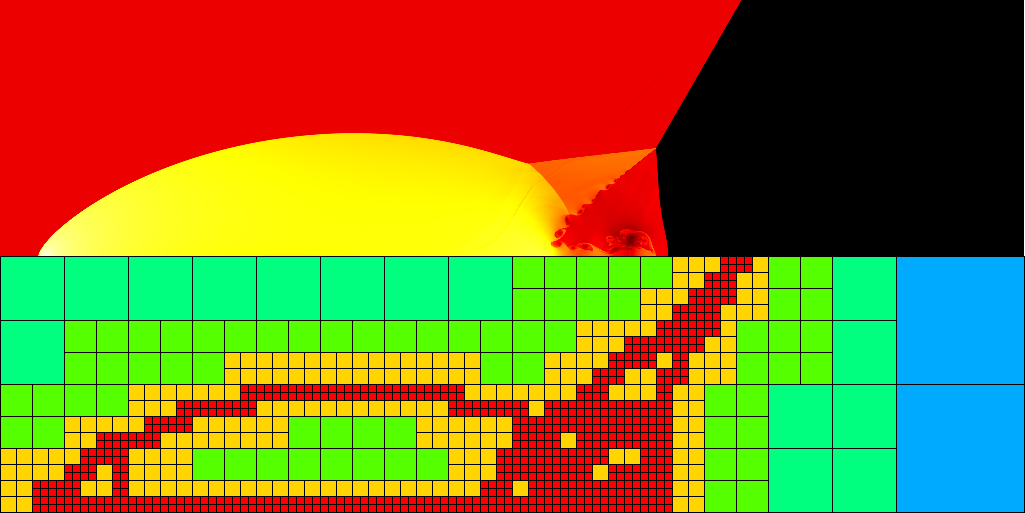
\includegraphics[width=4.0in]{Images/DoubleMachAmr/doublemach-0200.png}
%  % \ANIMATEGRAPHICS{width=4.5in}{20}{Images/DoubleMachAmr/doublemach-}{0000}{0307}
%  
%  
%  %    Boundary
%  %----------------------------------------------------------------------
%  
 \begin{frame}[fragile] 
 \secframetitle{\ssDoubleMach}
 \framesubtitle{\group{Boundary} conditions}
\footnotesize
\begin{semiverbatim}
 \group{Boundary} \{
    \variable{list} = [
            \valuetext{"OUT"},
            \valuetext{"REFLECT"},
            \valuetext{"DENSITY"},
            \valuetext{"VELOCITY_X"},
            \valuetext{"VELOCITY_Y"},
            \valuetext{"TOTAL_ENERGY}"
          ];
\}
\end{semiverbatim}
\end{frame}

%----------------------------------------------------------------------

 \begin{frame}[fragile] 
 \secframetitle{\ssDoubleMach}
 \framesubtitle{\group{Boundary} conditions: outflow and reflecting}
\footnotesize
\begin{semiverbatim}
 \group{Boundary} \{
    \subgroup{OUT} \{
       \variable{type} = \valuetext{"outflow"};
       \variable{mask} = [ (\variable{x} >= \valuetext{4.0}) || 
                (\variable{y} >= \valuetext{1.0} && (\variable{x} >= \valuetext{0.744017} + \valuetext{11.547}* \variable{t}))];
    \};
    \subgroup{REFLECT} \{
       \variable{type} = \valuetext{"reflecting"};
       \variable{axis} = \valuetext{"y"};
       \variable{face} = \valuetext{"lower"};
       \variable{mask} = (\variable{x} >= \valuetext{0.166667});
    \};
\} 
\end{semiverbatim}
\end{frame}

%----------------------------------------------------------------------

 \begin{frame}[fragile] 
 \secframetitle{\ssDoubleMach}
 \framesubtitle{\group{Boundary} conditions: \code{density}}
\footnotesize
\begin{semiverbatim}
\group{Boundary} \{
    \subgroup{DENSITY} \{
       \variable{type} = \valuetext{"inflow"};
       \variable{field_list} = \valuetext{"density"};
       \variable{value} = [ \valuetext{8.0}, 
                  ( (\variable{x} <= \valuetext{0.166667}) && (\variable{y} <= \valuetext{0.0}) ) ||
                    (\variable{x} <= \valuetext{0.0}) ||
                   ((\variable{x} <= \valuetext{0.744017} + \valuetext{11.547}*\variable{t)} && (\variable{y} >= \valuetext{1.0}))
               ];
    \};
\} 
\end{semiverbatim}
\end{frame}

%----------------------------------------------------------------------

 \begin{frame}[fragile] 
 \secframetitle{\ssDoubleMach}
 \framesubtitle{\group{Boundary} conditions: \code{velocity\_x}}
\footnotesize
\begin{semiverbatim}
\group{Boundary} \{
    \subgroup{VELOCITY_X} \{
       \variable{type} = \valuetext{"inflow"};
       \variable{field_list} = \valuetext{"velocity_x"};
       \variable{value} = [ \valuetext{8.25}*\valuetext{0.8660253},
                  ( (\variable{x} <= \valuetext{0.166667}) && (\variable{y} <= \valuetext{0.0}) ) ||
                    (\variable{x} <= \valuetext{0.0}) ||
                   ((\variable{x} <= \valuetext{0.744017} + \valuetext{11.547}*\variable{t)} && (\variable{y} >= \valuetext{1.0}))
               ];
    \};
\}
\end{semiverbatim}
\end{frame}

%----------------------------------------------------------------------

 \begin{frame}[fragile] 
 \secframetitle{\ssDoubleMach}
 \framesubtitle{\group{Boundary} conditions: \code{velocity\_y}}
\footnotesize
\begin{semiverbatim}
\group{Boundary} \{
    \subgroup{VELOCITY_Y} \{
       \variable{type} = \valuetext{"inflow"};
       \variable{field_list} = \valuetext{"velocity_y"};
       \variable{value} = [ -\valuetext{8.25}*\valuetext{0.5},
                  ( (\variable{x} <= \valuetext{0.166667}) && (\variable{y} <= \valuetext{0.0}) ) ||
                    (\variable{x} <= \valuetext{0.0}) ||
                   ((\variable{x} <= \valuetext{0.744017} + \valuetext{11.547}*\variable{t}) && (\variable{y} >= \valuetext{1.0}))
               ];
    \};
\}
\end{semiverbatim}
\end{frame}

%----------------------------------------------------------------------

 \begin{frame}[fragile] 
 \secframetitle{\ssDoubleMach}
 \framesubtitle{\group{Boundary} conditions: \code{total\_energy}}
\footnotesize
\begin{semiverbatim}
\group{Boundary} \{
    \subgroup{TOTAL_ENERGY} \{
       \variable{type} = \valuetext{"inflow"};
       \variable{field_list} = \valuetext{"total_energy"};
       \variable{value} = [ \valuetext{116.5} / (\valuetext{0.4} * \valuetext{8.0}) + \valuetext{34.03125},
                  ( (\variable{x} <= \valuetext{0.166667}) && (\variable{y} <= \valuetext{0.0}) ) ||
                    (\variable{x} <= \valuetext{0.0}) ||
                   ((\variable{x} <= \valuetext{0.744017} + \valuetext{11.547}*\variable{t)} && (\variable{y} >= \valuetext{1.0}))
               ];
    \};
\}
\end{semiverbatim}
\end{frame}

%----------------------------------------------------------------------

 \begin{frame}[fragile] 
 \secframetitle{\ssDoubleMach}
 \framesubtitle{Discretization: \group{Mesh} (forest) and \group{Adapt} (octrees)}
\footnotesize
%    Stopping
% \end{itemize}


\begin{semiverbatim}
\group{Mesh} \{
   \variable{root_rank} = \valuetext{2};
   \variable{root_size} = [\valuetext{96},\valuetext{24}];
   \variable{root_blocks} = [\valuetext{4},\valuetext{1}]; \comment{\# $24^2$ block size}
\}
\group{Adapt} \{
   \variable{max_level} = \valuetext{5}; 
   \variable{list} = [\valuetext{"SLOPE"}];
   \subgroup{SLOPE} \{
      \variable{type} = \valuetext{"slope"};
      \variable{field_list} = [\valuetext{"density"}];
      \variable{min_refine}  = \valuetext{5.0};
      \variable{max_coarsen} = \valuetext{2.0};
   \}
\}
\end{semiverbatim}
\end{frame}

%----------------------------------------------------------------------

 \begin{frame}[fragile] 
 \secframetitle{\ssDoubleMach}
 \framesubtitle{\group{Field} parameters}
\footnotesize
% 
% 
\begin{semiverbatim}
\group{Field} \{
   \variable{gamma} = \valuetext{1.4};
   \variable{list} = [
      \valuetext{"density"},        
      \valuetext{"velocity_x"},
      \valuetext{"velocity_y"},
      \valuetext{"total_energy"},
      \valuetext{"internal_energy"},
      \valuetext{"pressure"} ];
   \variable{ghost_depth} = \valuetext{4}; \comment{\# currently required by interpolation}
   \variable{courant}   = \valuetext{0.8};
\}
\end{semiverbatim}
\end{frame}

%----------------------------------------------------------------------

 \begin{frame}[fragile] 
 \secframetitle{\ssDoubleMach}
 \framesubtitle{\group{Method} parameters}
\footnotesize
\begin{semiverbatim}
\group{Method} \{
   \variable{list} = [\valuetext{"ppm"}];

   \subgroup{ppm} \{
      \variable{diffusion}   = \valuetext{true};
      \variable{flattening}  = \valuetext{3};
      \variable{steepening}  = \valuetext{true};
      \variable{dual_energy} = \valuetext{false};
  \}
\}
\end{semiverbatim}
\end{frame}

%----------------------------------------------------------------------

 \begin{frame}[fragile] 
 \secframetitle{\ssDoubleMach}
 \framesubtitle{\group{Output} parameters}
%\footnotesize
We wish to output
\begin{itemize}
\item HDF5 files of all data
\item density as an image
\item mesh refinement as an image
\end{itemize}

\begin{semiverbatim}
\group{Output} \{ 
   \variable{list} = [\valuetext{"hdf5"},\valuetext{"de_image"},\valuetext{"mesh_image"}];
\}
\end{semiverbatim}
\end{frame}

%----------------------------------------------------------------------

 \begin{frame}[fragile] 
 \secframetitle{\ssDoubleMach}
 \framesubtitle{\group{Output} data as HDF5}
\footnotesize
\begin{semiverbatim}
\group{Output} \{ 
   \subgroup{hdf5} \{
      \variable{type} = \valuetext{"data"};
      \variable{name} = [\valuetext{"doublemach-p%02d-c%04d.h5"}, \valuetext{"proc"},\valuetext{"count"}]; 
      \keyword{include} \valuetext{"input/schedule_cycle_25.incl"}
   \};
\}
\end{semiverbatim}
\end{frame}

%----------------------------------------------------------------------

 \begin{frame}[fragile] 
 \secframetitle{\ssDoubleMach}
 \framesubtitle{\group{Output} image of density}
\footnotesize
\begin{semiverbatim}
\group{Output} \{ 
   \subgroup{de_image} \{
      \variable{type} = \valuetext{"image"};
      \variable{name} = [\valuetext{"doublemach-de-%04d.png"}, \valuetext{"count"}]; 
      \variable{field_list} = [\valuetext{"density"}];
      \variable{image_size} = [\valuetext{1024},\valuetext{256}];
      \keyword{include} \valuetext{"input/schedule_cycle_25.incl"}
      \keyword{include} \valuetext{"input/colormap_blackbody.incl"}
   \};
\}
\end{semiverbatim}
\end{frame}

%----------------------------------------------------------------------

 \begin{frame}[fragile] 
 \secframetitle{\ssDoubleMach}
 \framesubtitle{\group{Output} image of mesh hierarchy}
\footnotesize

\begin{semiverbatim}
\group{Output} \{ 
    \subgroup{mesh_image} \{
        \variable{type}     = \valuetext{"image"};
        \variable{name} = [\valuetext{"doublemach-mesh-%04d.png"}, \valuetext{"count"}];
        \variable{image_type}  = \valuetext{"mesh"};
        \variable{image_reduce_type} = \valuetext{"max"};
        \variable{image_size} = [\valuetext{1025},\valuetext{257}];
        \keyword{include} \valuetext{"input/schedule_cycle_25.incl"}
        \variable{image_specify_bounds} = \valuetext{true};
        \variable{image_min} = \valuetext{0.0};
        \variable{image_max} = \valuetext{6.0};
        \keyword{include} \valuetext{"input/colormap_rainbow.incl"}
      \};
\}
\end{semiverbatim}
\end{frame}

%----------------------------------------------------------------------

\begin{frame}[fragile]
\secframetitle{\ssDoubleMach}
\footnotesize
\begin{center}
\ANIMATEGRAPHICS{width=4.0in}{20}{Images/DoubleMachAmr/doublemach-0}{000}{272}
\end{center}
\end{frame}

 % Double Mach Reflection
%%======================================================================
\NEWSEC
%======================================================================

\subsection{\ssRestart}

\begin{frame}[fragile,label=ss-restart] 
\secframetitle{\ssRestart}
\framesubtitle{Checkpointing to disk}
\footnotesize
\begin{tabbing}
xxxxxx\=xxxxxx\=xxxxxx\=\kill
\bluecode{Output \{} \\
\\
\>  \code{list = [}\bluecode{"check"}\code{];} \\
 \\
\>  \bluecode{check} \code{\{} \\
\>\>     \bluecode{type  = "checkpoint"}\code{;} \\
\>\>     \bluecode{dir   = ["checkpoint-\%d","count"];} \\
\>\>     \code{schedule \{} \\
\>\>\>   \code{var = }\bluecode{"seconds"}\code{;}\\
\>\>\>   \bluecode{start = 3600.0;} \\
\>\>\>   \bluecode{step  = 3600.0;} \\
\>\> \} \\
\>  \} \\
\}
\end{tabbing}
\end{frame}

%----------------------------------------------------------------------

\begin{frame}[fragile]
\secframetitle{\ssRestart}
\framesubtitle{Checkpointing to disk}
\tiny
\begin{semiverbatim}
\uncover<1->{\prompt \redcode{charmrun +p4 bin/enzo-p input/checkpoint_ppm-8.in}}\cursor{1}  
\vdots\uncover<2->{0 00001.75  -------------------------------------
0 00001.75 Simulation \bluetext{cycle 0000}
0 00001.75 Simulation time-sim 0.000000000000e+00
0 00001.75 Simulation dt 0.000000000000e+00
\vdots[0] \bluetext{Checkpoint starting in checkpoint_ppm-8-10}
0 00004.08 WARNING main.hpp:76
0 00004.08 WARNING Main::pup
0 00004.08 WARNING skipping monitor_
0 00004.08 WARNING parameters_Parameters.cpp:69
\vdots\bluetext{Checkpoint to disk finished in 0.854617s, sending out the cb...}
0 00006.37  -------------------------------------
0 00006.37 Simulation \bluetext{cycle 0010}
0 00006.37 Simulation time-sim 3.438861817873e-03
0 00006.37 Simulation dt 3.035398776372e-04
\vdots
}
\end{semiverbatim}
\end{frame}

%----------------------------------------------------------------------

\begin{frame}[fragile]
\secframetitle{\ssRestart}
\framesubtitle{Restarting from checkpoint}
\tiny
\begin{semiverbatim}
\uncover<1->{\prompt \redcode{ls checkpoint_ppm-8-10}}\cursor{1}
\uncover<2->{\bluecode{arr_0.dat  Chares_0.dat  Groups_0.dat  MainChares.dat	 NodeGroups_3.dat
arr_1.dat  Chares_1.dat  Groups_1.dat  NodeGroups_0.dat  RO.dat
arr_2.dat  Chares_2.dat  Groups_2.dat  NodeGroups_1.dat
arr_3.dat  Chares_3.dat  Groups_3.dat  NodeGroups_2.dat}}
\uncover<3->{\prompt \redcode{charmrun +p4 bin/enzo-p }\bluecode{+restart checkpoint_ppm-8-10}}\cursor{3}
\uncover<3->{\vdots0 00001.02 WARNING main.hpp:76
0 00001.02 WARNING Main::pup
0 00001.02 WARNING skipping monitor_
0 00001.02 WARNING parameters_Parameters.cpp:69
0 00001.02 WARNING Parameters::pup
\vdots\bluetext{[0]CkRestartMain done. sending out callback.}
0 00001.36  -------------------------------------
0 00001.36 Simulation \bluetext{cycle 0010}
0 00001.36 Simulation time-sim 3.438861817873e-03
0 00001.36 Simulation dt 3.035398776372e-04}
\vdots
\end{semiverbatim}
\end{frame}
%   
 % How do I restart from a checkpoint?
%%======================================================================
\NEWSEC
%======================================================================

\subsection{\ssLoadBalance}

\begin{frame}[fragile,label=ss-load-balance] 
\secframetitle{\ssLoadBalance}
\footnotesize
\begin{tabbing}
xxxxxx\=xxxxxx\=xxxxxx\=\kill
\bluecode{Balance \{} \\
\>     \code{schedule \{} \\
\>\>   \code{var = }\bluecode{"cycle"}\code{;}\\
\>\>   \bluecode{step  = 100;} \\
\> \} \\
\}
\end{tabbing}
\begin{semiverbatim}
\uncover<2->{\prompt \redcode{charmrun +p4 bin/enzo-p input/load-balance-4.in }\bluecode{+balancer RefineLB}}\cursor{2}
\end{semiverbatim}
\uncover<3->{\urltext{http://charm.cs.illinois.edu/manuals/html/charm++/7.html} \\
\textit{``The commonly used load balancers include }\bluecode{BlockLB}
\bluecode{ComboCentLB},
\bluecode{CommLB},
\bluecode{DistributedLB},
\bluecode{DummyLB},
\bluecode{GreedyCommLB},
\bluecode{GreedyLB},
\bluecode{HybridLB},
\bluecode{NeighborLB},
\bluecode{OrbLB},
\bluecode{RandCentLB},
\bluecode{RefineCommLB},
\bluecode{RefineLB},
\bluecode{RefineSwapLB},
\bluecode{RotateLB}.''}
\end{frame}

%----------------------------------------------------------------------

\begin{frame}[fragile]
\secframetitle{\ssLoadBalance}
\begin{center}
\begin{minipage}{1.3in}

\includegraphics[width=1.3in]{Images/Balance/balance-de-00000.png}
\end{minipage}
\begin{minipage}{1.3in}
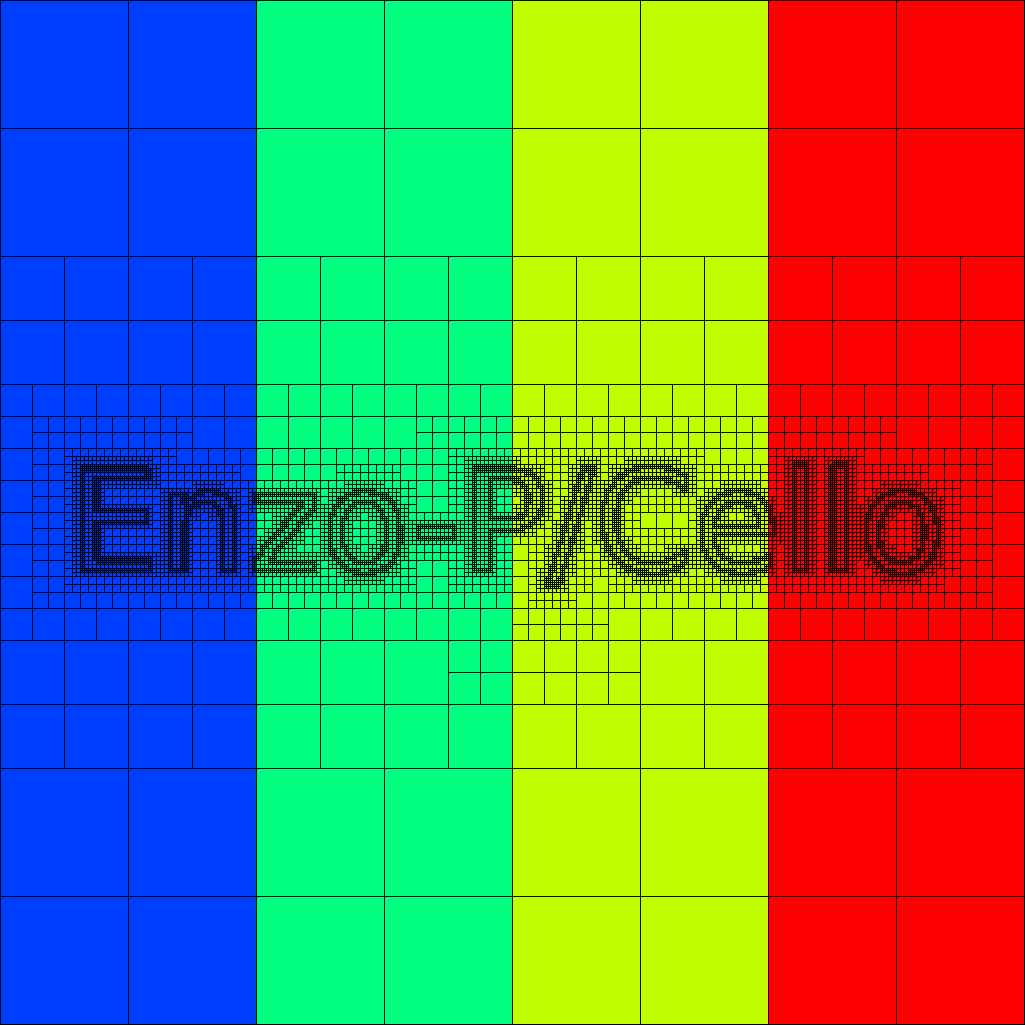
\includegraphics[width=1.3in]{Images/Balance/balance-mesh-00000.png}
\end{minipage}
\begin{minipage}{1.3in}

\includegraphics[width=1.3in]{Images/Balance/balance-mesh-00002.png}
\end{minipage}
\begin{minipage}{1.3in}
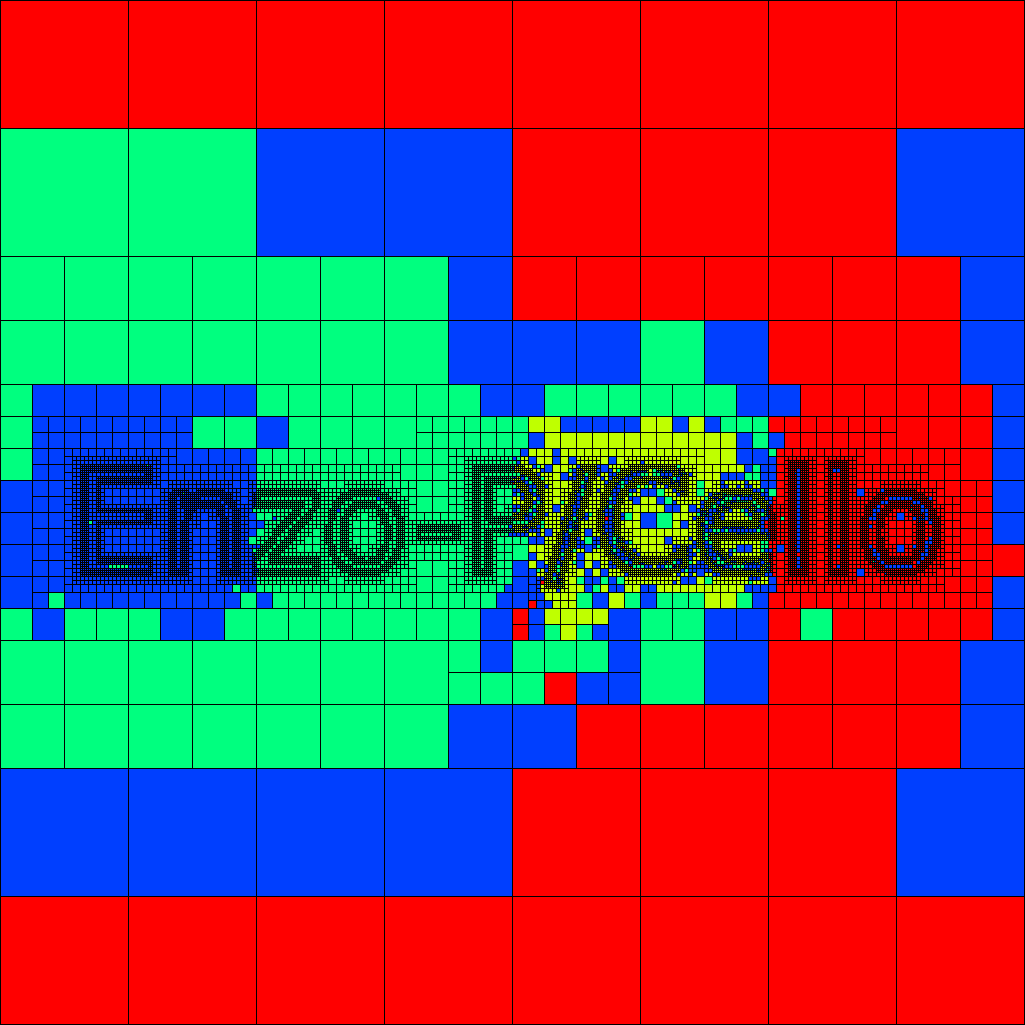
\includegraphics[width=1.3in]{Images/Balance/balance-mesh-00004.png}
\end{minipage}
\begin{minipage}{1.3in}
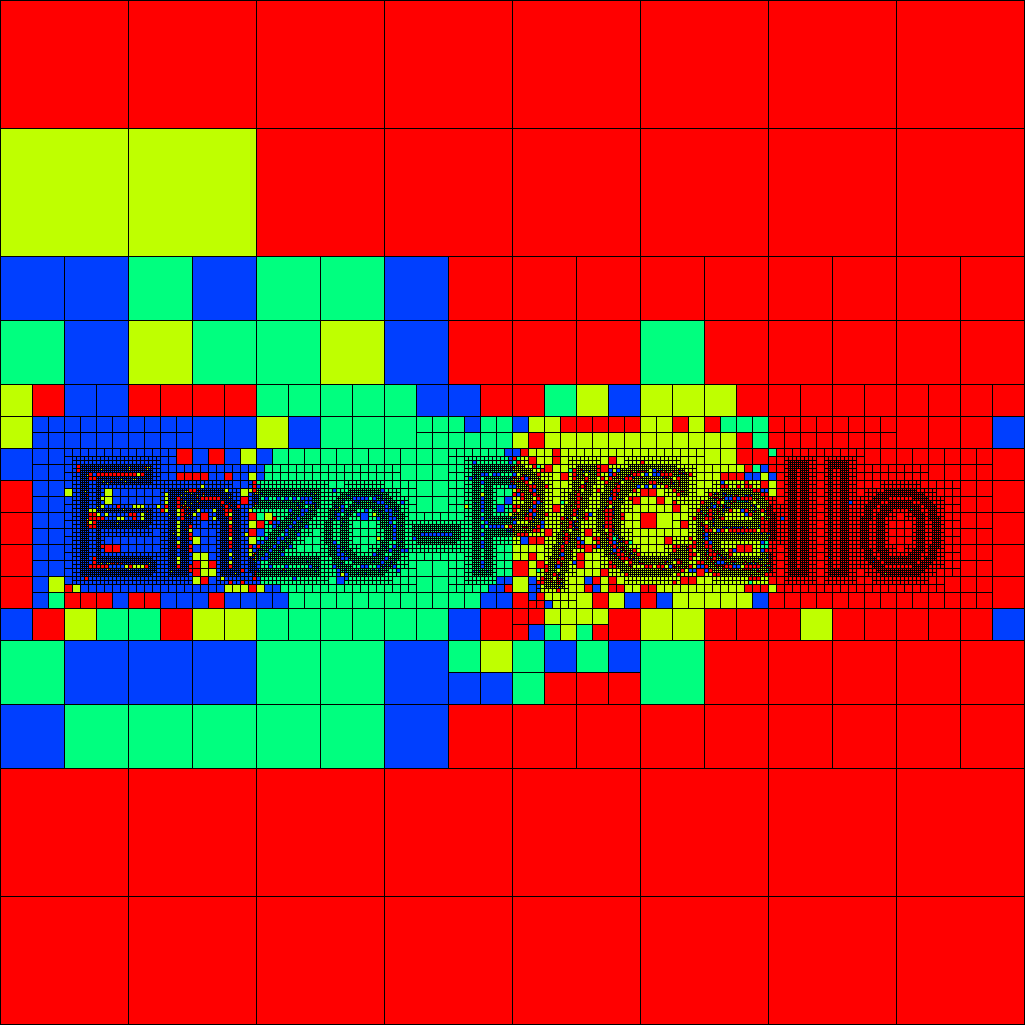
\includegraphics[width=1.3in]{Images/Balance/balance-mesh-00006.png}
\end{minipage}
\begin{minipage}{1.3in}
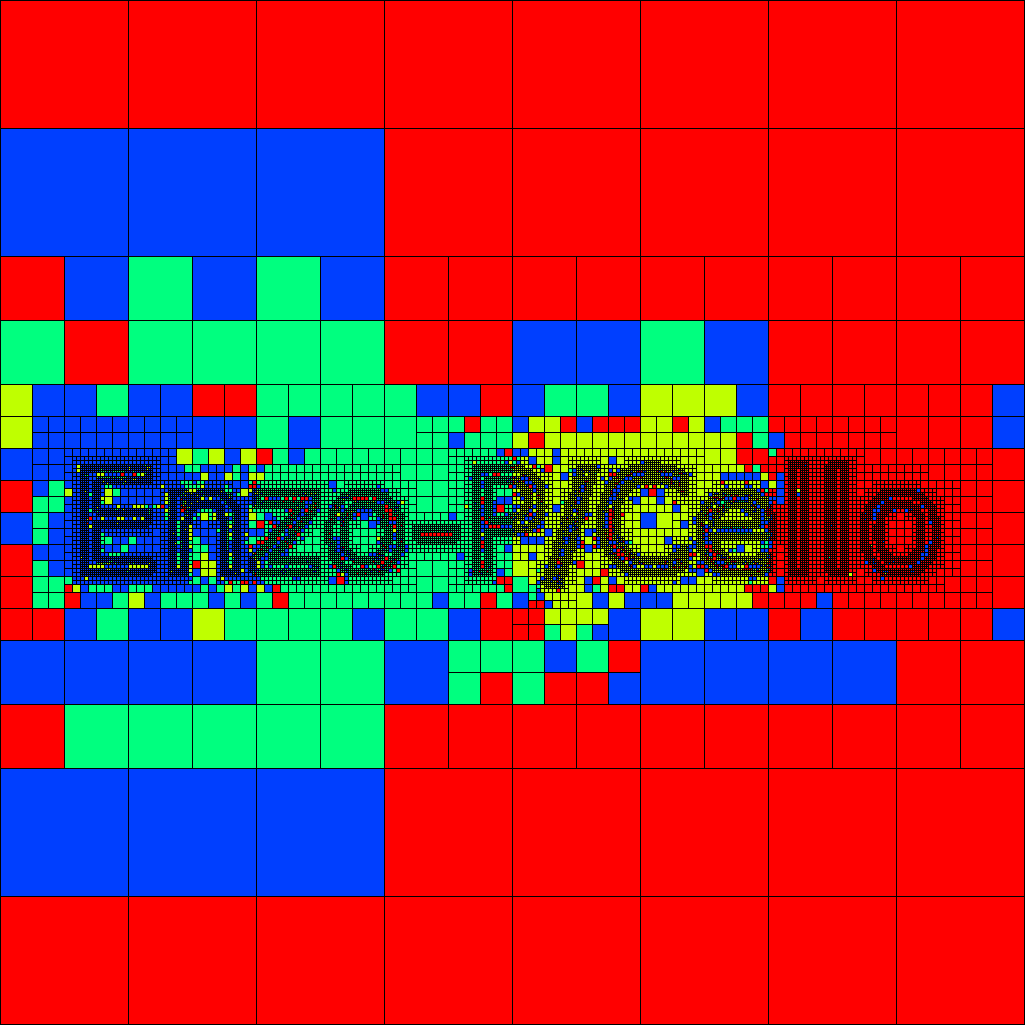
\includegraphics[width=1.3in]{Images/Balance/balance-mesh-00008.png}
\end{minipage}
\end{center}
\end{frame}
%----------------------------------------------------------------------



%     ComboCentLB : A special load balancer that can be used to combine any number of centralized load balancers mentioned above.

%     GreedyCommLB : Extends the greedy algorithm to take the communication graph into account.
%     GreedyLB : Uses a greedy algorithm that always assigns the heaviest object to the least loaded processor.
%     MetisLB : Uses METIS TM to partitioning object communication graph.
%     RandCentLB : Randomly assigns objects to processors;
%     RefineCommLB : Same idea as in RefineLB, but takes communication into account.
%     RefineLB : Moves objects away from the most overloaded processors to reach average, limits the number of objects migrated.
%     RefineSwapLB : Moves objects away from the most overloaded processors to reach average. In case it cannot migrate an object from an overloaded processor to an underloaded processor, it swaps objects to reduce the load on the overloaded processor. This strategy limits the number of objects migrated.
%     RefineTopoLB : Same idea as in RefineLB, but takes processor topology into account.
%     TopoCentLB : Extends the greedy algorithm to take processor topology into account.
 % How do run with dynamic load balancing?
%%======================================================================
\NEWSEC
%======================================================================

\subsection{\ssTools}

\begin{frame}[fragile,label=ss-tools] 
\secframetitle{\ssTools}

% ch-perf.py
% ch-perf.sh
% ch-swf.sh
% diff-org.sh
% grep-org.sh
% log-org.sh
% ls-org.sh
% plot_mesh.py
\begin{description}
\pause
\item[\code{./build.sh}] \ \\ compile \enzop, compile and/or run regression tests
\pause
\item[\code{./tools/org-diff.sh}] \ \\ Create \bluecode{diff.org} \code{org-mode} file from \bluecode{hg diff}
\pause
\item[\code{./tools/org-log.sh}] \ \\ Create \bluecode{log.org} \code{org-mode} file from \bluecode{hg log}
\pause
\item[\code{./tools/plot\_mesh.py}] \ \\ Plot octree forest given block id's (e.g. \textit{B0:000\_1:001})
\pause
\item[\code{./tools/ch-swf.sh}] \ \\ Generate SWF (flash) file given a sequence of PNG files
\end{description}
\end{frame}

%----------------------------------------------------------------------

% \begin{frame}[fragile] 
% \secframetitle{\ssTools}
% \framesubtitle{\code{build.sh}}
% \end{frame}

%----------------------------------------------------------------------

% \begin{frame}[fragile] 
% \secframetitle{\ssTools}
% \framesubtitle{\code{org-diff.sh}}
% \end{frame}

%----------------------------------------------------------------------

% \begin{frame}[fragile] 
% \secframetitle{\ssTools}
% \framesubtitle{\code{org-log.sh}}
% \end{frame}

%----------------------------------------------------------------------

% \begin{frame}[fragile] 
% \secframetitle{\ssTools}
% \framesubtitle{\code{plot\_mesh.py}}
% \end{frame}

%----------------------------------------------------------------------

% \begin{frame}[fragile] 
% \secframetitle{\ssTools}
% \framesubtitle{\code{ch-swf.sh}}
% \end{frame}

%       example: 
%       bin/enzo-p input/adapt-L5-P1.in
%        (Ctrl-C after adapt-0.h5, or edit input to add Schedule { cycle = 0; } (or wait))
%           h5ls adapt-0.h5 | head
%          B0:000_0:100             Group
%          B0:000_0:101             Group
%          B0:000_0:110             Group
%          B0:000_0:111             Group
%          B0:000_1:000             Group
%          B0:000_1:001             Group
%          B0:001_0:100             Group
%          B0:001_0:101             Group
%          B0:001_0:110             Group
%          B0:001_0:111             Group
%       h5ls adapt-0.h5 | tools/plot_mesh.py
%          explain e.g. B0:001_0:110
%    parse_error.awk

%    ch-mem.py
%    ch-mem.sh
%    ch-perf.py
%    ch-perf.sh
%    diff-org.awk
%    parse_ls.sh
%    parse_warning.awk


 % What tools does Cello provide?
%%======================================================================
\NEWSEC
%======================================================================

\subsection{\ssStartingSummary}

%----------------------------------------------------------------------

\begin{frame}[fragile,label=ss-starting-summary] 
\secframetitle{\ssStartingSummary}
\begin{itemize}
\item Enzo-P / Cello is easy (in principle) to download and install
\item Few dependencies
\begin{itemize}
\item \charm, HDF5, libpng, (csh,bc))
\end{itemize}
\item Not many platforms tested to date
\begin{itemize}
\item \redtext{Compiling issues are not unexpected!}
\item Your feedback is important!
\end{itemize}
\item Load-balancing requires command-line argument
\item Restarting requires checkpoint directory
\end{itemize}
\vfill
\centerline{$\qed$}
\end{frame}

 % What tools does Cello provide?


  %======================================================================
\NEWMOD
%======================================================================

\section{\sParameters}

%----------------------------------------------------------------------

\logo{\hfill\hyperlink{outline<1>}{\icon}}

\begin{frame}[fragile,label=s-parameters] 
\modframetitle{\sParameters}
\small
\begin{center}
\begin{minipage}{3.25in}
\begin{enumerate}
\item \hyperlink{ss-param-intro<1>}   {\BUTTON {\ssParamIntro}}
\item \hyperlink{ss-parameters<1>}   {\BUTTON {\ssParameters}}
\item \hyperlink{ss-doublemach<1>}     {\BUTTON {\ssDoubleMach}}
% \item \hyperlink{ss-param-problem<1>}   {\BUTTON {\ssParamProblem}}
% \item \hyperlink{ss-param-refine<1>}   {\BUTTON {\ssParamRefine}}
% \item \hyperlink{ss-param-data<1>}   {\BUTTON {\ssParamData}}
% \item \hyperlink{ss-param-method<1>}   {\BUTTON {\ssParamMethod}}
% \item \hyperlink{ss-param-io<1>}   {\BUTTON {\ssParamIo}}
% \item \hyperlink{ss-param-other<1>}   {\BUTTON {\ssParamOther}}
\item \hyperlink{ss-param-activity<1>}     {\BUTTON {\ssParamActivity}}
\item \hyperlink{ss-parameters-summary<1>}     {\BUTTON {\ssParametersSummary}}
\end{enumerate}
\end{minipage}
\end{center}
\end{frame}

\logo{\hfill\hyperlink{s-parameters<1>}{\icon}}

%======================================================================
\NEWSEC
%======================================================================

\subsection{\ssParamIntro}

\begin{frame}[fragile,label=ss-param-intro] 
\secframetitle{\ssParamIntro}
\framesubtitle{Introduction to Enzo-P/Cello parameter files}
\textbf{Enzo-P uses \textit{structured} parameter files}
\footnotesize
\pause
\begin{itemize}
\item \parameter{parameters} are organized into \group{Groups} and \subgroup{subgroups}
\pause
\begin{minipage}{3in}
\vspace{0.1in}
\begin{semiverbatim}
\group{Initial} \{
    list = ["value"];
    \subgroup{value} \{
       \parameter{velocity_x = 1.0};
   \}
\}
\end{semiverbatim}
\end{minipage}
\pause
\item parameters have a variety of types
\pause
\begin{minipage}{3in}
\vspace{0.1in}
  \begin{tabbing}
xxxxxxxxxxxxxxxxx\=xxxxxxxxxxxxxxxxxx\=\kill
\>  \uncover<5->{\textit{floating-point}:} \' \uncover<5->{\parameter{value} \texttt{=} \valuetext{1.0};} \\
\>  \uncover<6->{\textit{integers}:} \' \uncover<6->{\parameter{cycle} \texttt{=} \valuetext{100};} \\
\>  \uncover<7->{\textit{logical}:} \' \uncover<7->{\parameter{crash} \texttt{=} \valuetext{false};} \\
\>  \uncover<8->{\textit{string}:} \' \uncover<8->{\parameter{type} \texttt{=} \valuetext{"dinosaur"};} \\
\>  \uncover<9->{\textit{lists}:} \' \uncover<9->{\parameter{list} \texttt{=} \valuetext{["density", "gravity"]};} \\
\>  \uncover<10->{\textit{FP-expressions}:} \'  \uncover<10->{\parameter{value} \texttt{=} \valuetext{1.0 + 3.0*sin(x)};} \\
\>  \uncover<11->{\textit{logical-expressions}:} \' \uncover<11->{\parameter{mask} \texttt{=} \valuetext{(x >= 4.0) || (y >= 1.0)};}
\end{tabbing}
\end{minipage}
\end{itemize}
\end{frame}

%======================================================================

\begin{frame}[fragile]
\secframetitle{\ssParamIntro}
\framesubtitle{Introduction to Enzo-P/Cello parameter files}
\footnotesize
\begin{itemize}
\item Groups can be disjoint
\pause
\begin{semiverbatim}
\uncover<+->{\group{Method} \{
   \parameter{list} = \valuetext{["ppm"]};
\}}
\uncover<+->{\group{Method} \{
   \subgroup{ppm} \{
       \parameter{dual_energy} = \valuetext{true};
    \}
\}}
\end{semiverbatim}
\uncover<+->{\item Multiple parameter assignments use last value}
\begin{semiverbatim}
\uncover<+->{\parameter{list} = \valuetext{["ppm", "gravity"];}}
\uncover<+->{\parameter{list} = \valuetext{["gravity","ppm"];} \textsf{\comment{\# this value used}}}
\uncover<+->{\parameter{list} += \valuetext{["pm_update"];} \textsf{\comment{\# lists can be appended to}}}
\end{semiverbatim}
\uncover<+->{\item \comment{\# Hi! I'm a comment.}}
\end{itemize}
\end{frame}

%======================================================================



\begin{frame}[fragile] 
\secframetitle{\ssParamIntro}
\framesubtitle{Introduction to Enzo-P/Cello parameter files}

\begin{itemize}
\uncover<+->{\item Files can be \bluecode{included}}
\begin{semiverbatim}
\uncover<+->{\group{Output \{ }
   \subgroup{density} \{
      \bluecode{include} \valuetext{"input/schedule_cycle_100.incl"}
   \}
\}}
\end{semiverbatim}
\uncover<+->{\item Complicated ``including'' of files can be confusing}
\uncover<+->{\item Cello outputs a \greencode{parameters.out} file}
\begin{itemize}
\uncover<+->{\item contains all parameters}
\uncover<+->{\item organized alphabetically}
\uncover<+->{\item can be used as an input parameter file}
\end{itemize}
\end{itemize}

\end{frame}
%======================================================================


\begin{frame}[fragile]
\secframetitle{\ssParamIntro}
\framesubtitle{Parameter file issues}
% Review ss-bugs.tex / http://client64-249.sdsc.edu/cello-bug

\begin{itemize}
   \item Floats and integers cannot be mixed
   \cornersize{0.9}
   \begin{itemize}
     \item[\frownie] \textcolor{red}{\code{velocity\_x = 8.0 + 2*x }}
     \item[\smiley] \textcolor{green!50!black}{\code{velocity\_x = 8.0 + 2.0*x}}
   \end{itemize}

   \item Need space after subtraction minus sign
   \begin{itemize}
     \item[\frownie] \textcolor{red}{\code{density = x -2.0;}}
     \item[\smiley] \textcolor{green!50!black}{\code{density = x - 2.0;}}
   \end{itemize}
  \item Need at least as many root blocks as processors $P$
  \begin{itemize}
    \item \code{Mesh \{ root\_blocks = [4,4,4]; \} }
    \item[\frownie] \textcolor{red}{\code{\$ charmrun +p72} \code{bin/enzo-p \ldots}}
    \item[\smiley]\textcolor{green!50!black}{\code{\$ charmrun +p64} \code{bin/enzo-p \ldots}}
  \end{itemize}
  \item AMR requires ghost zone depth of $\ge 4$
\end{itemize}

\link{ss-bugs}{Other issues: see bug tracking website}

\end{frame}

 % Enzo-P / Cello parameter files
%======================================================================
\NEWSEC
%======================================================================

\subsection{\ssParameters}

\begin{frame}[fragile,label=ss-parameters] 
\secframetitle{\ssParameters}
\framesubtitle{Writing parameter files by \group{Group}}
\vspace{-0.2in}
\begin{minipage}[t]{1.7in}
\begin{itemize}
\item 
\textcolor{blue}{Problem definition}
  \begin{itemize}
\pause
\item
\begin{tabbing}
xxxxxxxxxxxxxxxxxxxxxxxxxx\=\kill
  \textcolor{blue}{\code{Domain}} \> \blueit{domain extents}
\end{tabbing}
\item \begin{tabbing}
xxxxxxxxxxxxxxxxxxxxxxxxxx\=\kill
  \textcolor{blue}{\code{Initial}} \> \blueit{initial conditions}
\end{tabbing}
\item \begin{tabbing}
xxxxxxxxxxxxxxxxxxxxxxxxxx\=\kill
  \textcolor{blue}{\code{Boundary}} \> \blueit{boundary conditions}
\end{tabbing}
\pause
  \item \begin{tabbing}
xxxxxxxxxxxxxxxxxxxxxxxxxx\=\kill
 \textcolor{blue}{\code{Stopping}} \> \blueit{stopping criteria}
\end{tabbing}
  \end{itemize}
\pause
\item \textcolor{green!50!black}{Discretization}
  \begin{itemize}
  \item \begin{tabbing}
xxxxxxxxxxxxxxxxxxxxxxxxxx\=\kill
 \textcolor{green!50!black}{\code{Mesh}} \> \greenit{root mesh blocking}
  \end{tabbing}  
  \item \begin{tabbing}
xxxxxxxxxxxxxxxxxxxxxxxxxx\=\kill
 \textcolor{green!50!black}{\code{Adapt}} \> \greenit{adaptive mesh refinement}
   \end{tabbing}
\pause
  \item \begin{tabbing}
xxxxxxxxxxxxxxxxxxxxxxxxxx\=\kill
 \textcolor{green!50!black}{\code{Field}} \> \greenit{field data}
   \end{tabbing}
  \end{itemize}
\pause
\item \textcolor{red!50!black}{Parallel computation}
  \begin{itemize}
\pause
  \item \begin{tabbing}
xxxxxxxxxxxxxxxxxxxxxxxxxx\=\kill
 \textcolor{red!50!black}{\code{Method}} \> \redit{computational methods}
  \end{tabbing}
  \end{itemize}
\pause
\item \textcolor{cyan!50!black}{Output}
  \begin{itemize}
\pause
    \item \begin{tabbing}
xxxxxxxxxxxxxxxxxxxxxxxxxx\=\kill
 \textcolor{cyan!50!black}{\code{Output}} \> \cyanit{disk output}
    \end{tabbing}
  \end{itemize}
\end{itemize}
\end{minipage}
\end{frame}

%======================================================================
% \secframetitle{\ssParameters}
% \framesubtitle{\ }
% \begin{minipage}[t]{1.7in}
% \begin{itemize}
% \item \textcolor{blue}{Problem definition}
%   \begin{itemize}
%   \item \textcolor{blue}{\code{Domain}}
%   \item \textcolor{blue}{\code{Initial}}
%   \item \textcolor{blue}{\code{Boundary}}
%   \item \textcolor{blue}{\code{Stopping}}
%   \end{itemize}
% \item \textcolor<1>{green!50!black}{Discretization}
%   \begin{itemize}
%   \item \textcolor<1>{green!50!black}{\code{Mesh}}
%   \item \textcolor<1>{green!50!black}{\code{Adapt}}
%   \item \textcolor<1>{green!50!black}{\code{Field}}
%   \end{itemize}
% \item \textcolor<1>{red!50!black}{Parallel computation}
%   \begin{itemize}
%   \item \textcolor<1>{red!50!black}{\code{Method}}
%   \end{itemize}
% \item \textcolor<1>{cyan!50!black}{Output}
%   \begin{itemize}
%     \item \textcolor<1>{cyan!50!black}{\code{Output}}
%   \end{itemize}
% \end{itemize}
% \end{minipage}
% \end{frame}

%----------------------------------------------------------------------

\begin{frame}[fragile] 
\secframetitle{\ssParameters}
\framesubtitle{Problem parameters}
\vspace{-0.2in}
\begin{minipage}[t]{1.7in}
\begin{itemize}
\item \bfat{1}{\textcolor{blue}{Problem definition}}
  \begin{itemize}
  \item \bfat{1}{\textcolor{blue}{\code{Domain}}}
  \item \textcolor{blue}{\code{Initial}}
  \item \textcolor{blue}{\code{Boundary}}
  \item \textcolor{blue}{\code{Stopping}}
  \end{itemize}
\item Discretization
  \begin{itemize}
  \item \code{Mesh}
  \item \code{Adapt}
  \item \code{Field}
  \end{itemize}
\item Parallel computation
  \begin{itemize}
  \item \code{Method}
  \end{itemize}
\item Output
  \begin{itemize}
    \item \code{Output}
  \end{itemize}
\end{itemize}
\end{minipage} \
%- - - - - - - - - - - - - - - - - - -
\begin{minipage}[t]{2.6in}
\vspace{-0.2in}
\setbeamercolor{block title}{bg=blue!30,fg=black}
\begin{block}{\textbf{Domain definition}}
\footnotesize \vspace{-0.1in}
\begin{semiverbatim}
\group{Domain} \{
   \variable{lower} = [\valuetext{0.0}, \valuetext{0.0}];
   \variable{upper} = [\valuetext{0.3}, \valuetext{0.3}];
\} 
\end{semiverbatim}
\end{block}
\end{minipage}
\end{frame}


%----------------------------------------------------------------------

\begin{frame}[fragile] 
\secframetitle{\ssParameters}
\framesubtitle{Problem parameters}
\vspace{-0.2in}
\begin{minipage}[t]{1.7in}
\begin{itemize}
\item \bfat{1}{\textcolor{blue}{Problem definition}}
  \begin{itemize}
  \item \textcolor{blue}{\code{Domain}}
  \item \bfat{1}{\textcolor{blue}{\code{Initial}}}
  \item \textcolor{blue}{\code{Boundary}}
  \item \textcolor{blue}{\code{Stopping}}
  \end{itemize}
\item Discretization
  \begin{itemize}
  \item \code{Mesh}
  \item \code{Adapt}
  \item \code{Field}
  \end{itemize}
\item Parallel computation
  \begin{itemize}
  \item \code{Method}
  \end{itemize}
\item Output
  \begin{itemize}
    \item \code{Output}
  \end{itemize}
\end{itemize}
\end{minipage} \
%- - - - - - - - - - - - - - - - - - -
\begin{minipage}[t]{2.6in}
\vspace{-0.2in}
\setbeamercolor{block title}{bg=blue!30,fg=black}
\begin{block}{\textbf{Initial Conditions}}
\footnotesize \vspace{-0.1in}
\begin{semiverbatim}
\group{Initial} \{
   \variable{type} = \valuetext{"value"};
   \subgroup{density} \{
      \variable{value} = [ \valuetext{0.125},   \variable{x} +  \variable{y} <  \valuetext{0.15}, 
                \valuetext{1.0} ];
   \};
   \subgroup{total_energy} \{
        \variable{value} = [  \valuetext{0.14} / ( \valuetext{0.4} *  \valuetext{0.125}),
                     \variable{x} +  \variable{y} <  \valuetext{0.15},
                  \valuetext{1.00} / ( \valuetext{0.4} *  \valuetext{1.000}) ];
   \};
\}
\end{semiverbatim}
\end{block}
\end{minipage}
\end{frame}

\begin{frame}[fragile] 
\secframetitle{\ssParameters}
\framesubtitle{Problem parameters}
\vspace{-0.2in}
\begin{minipage}[t]{1.7in}
\begin{itemize}
\item \bfat{1}{\textcolor{blue}{Problem definition}}
  \begin{itemize}
  \item \textcolor{blue}{\code{Domain}}
  \item \textcolor{blue}{\code{Initial}}
  \item \bfat{1}{\textcolor{blue}{\code{Boundary}}}
  \item \bfat{2}{\textcolor{blue}{\code{Stopping}}}
  \end{itemize}
\item Discretization
  \begin{itemize}
  \item \code{Mesh}
  \item \code{Adapt}
  \item \code{Field}
  \end{itemize}
\item Parallel computation
  \begin{itemize}
  \item \code{Method}
  \end{itemize}
\item Output
  \begin{itemize}
    \item \code{Output}
  \end{itemize}
\end{itemize}
\end{minipage} \
%- - - - - - - - - - - - - - - - - - -
\begin{minipage}[t]{2.6in}
\vspace{-0.2in}
\setbeamercolor{block title}{bg=blue!30,fg=black}
 \begin{block}<+->{\textbf{Boundary conditions}}
 \footnotesize \vspace{-0.1in}
 \begin{semiverbatim}
\group{Boundary} \{
   \variable{list} = [\valuetext{"x_bc"}, \valuetext{"y_bc"}];
   \subgroup{x_bc} \{ \variable{axis} = \valuetext{"x"}; \variable{type} = \valuetext{"reflecting"}; \};
   \subgroup{y_bc} \{ \variable{axis} = \valuetext{"y"}; \variable{type} = \valuetext{"periodic"}; \};
\}
 \end{semiverbatim}
 \end{block}
 \begin{block}<+->{\textbf{Stopping criteria}}
 \footnotesize \vspace{-0.1in}
 \begin{semiverbatim}
 \group{Stopping} \{ \variable{cycle} = \valuetext{100}; \}
 \end{semiverbatim}
 \end{block}
\end{minipage}
\end{frame}

%----------------------------------------------------------------------

\begin{frame}[fragile] 
\secframetitle{\ssParameters}
\framesubtitle{Discretization parameters}
\vspace{-0.2in}
\begin{minipage}[t]{1.7in}
\begin{itemize}
\item Problem definition
  \begin{itemize}
  \item \code{Domain}
  \item \code{Initial}
  \item \code{Boundary}
  \item \code{Stopping}
  \end{itemize}
\item \bfat{1-2}{\textcolor{green!50!black}{Discretization}}
  \begin{itemize}
  \item \bfat{1}{\textcolor{green!50!black}{\code{Mesh}}}
  \item \bfat{2}{\textcolor{green!50!black}{\code{Adapt}}}
  \item \textcolor{green!50!black}{\code{Field}}
  \end{itemize}
\item Parallel computation
  \begin{itemize}
  \item \code{Method}
  \end{itemize}
\item Output
  \begin{itemize}
    \item \code{Output}
  \end{itemize}
\end{itemize}
\end{minipage} \
%- - - - - - - - - - - - - - - - - - -
\begin{minipage}[t]{2.6in}
\vspace{-0.2in}
\setbeamercolor{block title}{bg=green!30,fg=black}
\begin{block}<+->{\textbf{Mesh hierarchy control}}
  \footnotesize \vspace{-0.1in}
\begin{semiverbatim}
\group{Mesh} \{ 
   \variable{root_rank}   = \valuetext{2};
   \variable{root_size}   = [\valuetext{400},\valuetext{400}];
   \variable{root_blocks} = [\valuetext{4},\valuetext{4}];
\}
\end{semiverbatim}
\begin{semiverbatim}
\uncover<2->{\group{Adapt} \{
   \variable{max_level} = \valuetext{5};
   \variable{list} = [\valuetext{"SLOPE"}];
   \subgroup{SLOPE} \{
      \variable{type} = \valuetext{"slope"};
      \variable{field_list} = [\valuetext{"density"}];
   \}
\}
}
\end{semiverbatim}
\end{block}
\end{minipage}
\end{frame}

%----------------------------------------------------------------------

\begin{frame}[fragile] 
\secframetitle{\ssParameters}
\framesubtitle{Discretization parameters}
\vspace{-0.2in}
\begin{minipage}[t]{1.7in}
\begin{itemize}
\item Problem definition
  \begin{itemize}
  \item \code{Domain}
  \item \code{Initial}
  \item \code{Boundary}
  \item \code{Stopping}
  \end{itemize}
\item \bfat{1}{\textcolor{green!50!black}{Discretization}}
  \begin{itemize}
  \item \textcolor{green!50!black}{\code{Mesh}}
  \item \textcolor{green!50!black}{\code{Adapt}}
  \item \bfat{1}{\textcolor{green!50!black}{\code{Field}}}
  \end{itemize}
\item Parallel computation
  \begin{itemize}
  \item \code{Method}
  \end{itemize}
\item Output
  \begin{itemize}
    \item \code{Output}
  \end{itemize}
\end{itemize}
\end{minipage} \
%- - - - - - - - - - - - - - - - - - -
\begin{minipage}[t]{2.6in}
\vspace{-0.2in}
\setbeamercolor{block title}{bg=green!30,fg=black}
  \begin{block}<+->{\textbf{Field variables}}
  \footnotesize \vspace{-0.1in}
\begin{semiverbatim}
\group{Field} \{
   \variable{list} = [\valuetext{"density"},
           \valuetext{"velocity_x"},
           \valuetext{"velocity_y"},
           \valuetext{"total_energy"},
           \valuetext{"pressure"}];
   \variable{courant}   = \valuetext{0.8};
   \variable{ghosts}    = \valuetext{3};
   \variable{alignment} = \valuetext{8};    
\}
\end{semiverbatim}
\end{block}
\end{minipage}
\end{frame}
  

%----------------------------------------------------------------------

\begin{frame}[fragile] 
\secframetitle{\ssParameters}
 \framesubtitle{Parallel computation parameters}
\vspace{-0.2in}
\begin{minipage}[t]{1.80in}
\begin{itemize}
\item Problem definition
  \begin{itemize}
  \item \code{Domain}
  \item \code{Initial}
  \item \code{Boundary}
  \item \code{Stopping}
  \end{itemize}
\item Discretization
  \begin{itemize}
  \item \code{Mesh}
  \item \code{Adapt}
  \item \code{Field}
  \end{itemize}
\item \bfat{1}{\textcolor{red!50!black}{Parallel computation}}
  \begin{itemize}
  \item \bfat{1}{\textcolor{red!50!black}{\code{Method}}}
  \end{itemize}
\item Output
  \begin{itemize}
    \item \code{Output}
  \end{itemize}
\end{itemize}
\end{minipage} \
%- - - - - - - - - - - - - - - - - - -
%- - - - - - - - - - - - - - - - - - -
\begin{minipage}[t]{2.50in}
\vspace{-0.2in}
\setbeamercolor{block title}{bg=red!30,fg=black}
 \begin{block}<+->{\textbf{Method list}}
 \footnotesize \vspace{-0.1in}
\begin{semiverbatim}
\group{Method} \{
   \variable{list} = [\valuetext{"ppm"},\valuetext{"gravity_bicgstab"}];
   \subgroup{ppm} \{
      \variable{diffusion}   = \valuetext{true};
      \variable{steepening}  = \valuetext{true};
   \};
   \subgroup{gravity_bicgstab} \{
      \variable{iter_max} = \valuetext{100};
      \variable{res_tol}  = \valuetext{0.001};
   \}
\}
\end{semiverbatim}
\end{block}
\end{minipage}
\end{frame}

%----------------------------------------------------------------------

% \begin{frame}[fragile] 
% \secframetitle{\ssParameters}
%  \framesubtitle{Parallel computation parameters}
% \vspace{-0.2in}
% \begin{minipage}[t]{1.80in}
% \begin{itemize}
% \item Problem definition
%   \begin{itemize}
%   \item \code{Domain}
%   \item \code{Initial}
%   \item \code{Boundary}
%   \item \code{Stopping}
%   \end{itemize}
% \item Discretization
%   \begin{itemize}
%   \item \code{Mesh}
%   \item \code{Adapt}
%   \item \code{Field}
%   \end{itemize}
% \item \bfat{1}{\textcolor{red!50!black}{Parallel computation}}
%   \begin{itemize}
%   \item \code{Method}
%   \end{itemize}
% \item Output
%   \begin{itemize}
%     \item \code{Output}
%   \end{itemize}
% \end{itemize}
% \end{minipage} \
%- - - - - - - - - - - - - - - - - - -
%- - - - - - - - - - - - - - - - - - -
% \begin{minipage}[t]{2.50in}
% \vspace{-0.2in}
% \setbeamercolor{block title}{bg=red!30,fg=black}
%  \begin{block}<+->{\textbf{Refresh list}}
%  \footnotesize \vspace{-0.1in}
% \begin{verbatim}
% Refresh {
%    list = ["ppm_refresh"];
%    ppm_refresh { 
%       field_face_rank = 0;
%       field_ghosts = 4;
%    }
% }
% \end{verbatim}
% \end{block}
% \end{minipage}
% \end{frame}

%----------------------------------------------------------------------

\begin{frame}[fragile] 
\secframetitle{\ssParameters}
\framesubtitle{Output parameters}
\vspace{-0.2in}
\begin{minipage}[t]{1.7in}
\begin{itemize}
\item Problem definition
  \begin{itemize}
  \item \code{Domain}
  \item \code{Initial}
  \item \code{Boundary}
  \item \code{Stopping}
  \end{itemize}
\item Discretization
  \begin{itemize}
  \item \code{Mesh}
  \item \code{Adapt}
  \item \code{Field}
  \end{itemize}
\item Parallel computation
  \begin{itemize}
  \item \code{Method}
  \end{itemize}
\item \bfat{1}{\textcolor{cyan!50!black}{Output}}
  \begin{itemize}
    \item \bfat{1}{\textcolor{cyan!50!black}{\code{Output}}}
  \end{itemize}
\end{itemize}
\end{minipage} \
%- - - - - - - - - - - - - - - - - - -
%- - - - - - - - - - - - - - - - - - -
\begin{minipage}[t]{2.6in}
\vspace{-0.2in}
\setbeamercolor{block title}{bg=cyan!50,fg=black}
 \begin{block}<+->{\textbf{Output files}}
 \footnotesize \vspace{-0.1in}
\begin{semiverbatim}
\group{Output} \{
   \variable{list} = [ \valuetext{"de_hdf5"}, \valuetext{"de_png"} ];
   \subgroup{de_hdf5} \{
      \comment{\# HDF5 data file group}
   \};
   \subgroup{de_png} \{
      \comment{\# PNG image file group}
   \}
\}
\end{semiverbatim}
 \end{block}
 \end{minipage}
\end{frame}
 
%----------------------------------------------------------------------
 
\begin{frame}[fragile] 
\secframetitle{\ssParameters}
\framesubtitle{Output parameters}
\vspace{-0.2in}
\begin{minipage}[t]{1.7in}
\begin{itemize}
\item Problem definition
  \begin{itemize}
  \item \code{Domain}
  \item \code{Initial}
  \item \code{Boundary}
  \item \code{Stopping}
  \end{itemize}
\item Discretization
  \begin{itemize}
  \item \code{Mesh}
  \item \code{Adapt}
  \item \code{Field}
  \end{itemize}
\item Parallel computation
  \begin{itemize}
  \item \code{Method}
  \end{itemize}
\item \bfat{1}{\textcolor{cyan!50!black}{Output}}
  \begin{itemize}
    \item \bfat{1}{\textcolor{cyan!50!black}{\code{Output}}}
  \end{itemize}
\end{itemize}
\end{minipage} \
%- - - - - - - - - - - - - - - - - - -
%- - - - - - - - - - - - - - - - - - -
\begin{minipage}[t]{2.6in}
\vspace{-0.2in}
\setbeamercolor{block title}{bg=cyan!50,fg=black}
 \begin{block}<+->{\textbf{Output files}}
 \footnotesize \vspace{-0.1in}
\begin{semiverbatim}
\group{Output} \{
   \subgroup{de_hdf5} \{
      \variable{type} = \valuetext{"data"};
      \variable{name} = [\valuetext{"implosion-%5.2f.png"},
              \valuetext{"time"}];
      \variable{field_list} = [\valuetext{"density"}];
      \subgroup{schedule} \{
         \variable{var}  = \valuetext{"time"};
         \variable{step} = \valuetext{0.02};
      \}
   \}
\}
\end{semiverbatim}
\end{block}
\end{minipage}
\end{frame}

%----------------------------------------------------------------------
 
\begin{frame}[fragile] 
\secframetitle{\ssParameters}
\framesubtitle{Output parameters}
\vspace{-0.2in}
\begin{minipage}[t]{1.7in}
\begin{itemize}
\item Problem definition
  \begin{itemize}
  \item \code{Domain}
  \item \code{Initial}
  \item \code{Boundary}
  \item \code{Stopping}
  \end{itemize}
\item Discretization
  \begin{itemize}
  \item \code{Mesh}
  \item \code{Adapt}
  \item \code{Field}
  \end{itemize}
\item Parallel computation
  \begin{itemize}
  \item \code{Method}
  \end{itemize}
\item \bfat{1}{\textcolor{cyan!50!black}{Output}}
  \begin{itemize}
    \item \bfat{1}{\textcolor{cyan!50!black}{\code{Output}}}
  \end{itemize}
\end{itemize}
\end{minipage} \
%- - - - - - - - - - - - - - - - - - -
%- - - - - - - - - - - - - - - - - - -
\begin{minipage}[t]{2.6in}
\vspace{-0.2in}
\setbeamercolor{block title}{bg=cyan!50,fg=black}
 \begin{block}<+->{\textbf{Output files}}
 \footnotesize \vspace{-0.1in}
 \begin{semiverbatim}
\group{Output} \{
   \subgroup{de_png} \{
      \variable{type} = \valuetext{"image"};
      \variable{name} = [ \valuetext{"implosion-%05d.png"},
               \valuetext{"cycle"} ];
      \variable{image_type} = \valuetext{"data"};
      \variable{colormap} = [\valuetext{0.0},\valuetext{0.0},\valuetext{0.0},
                  \valuetext{1.0},\valuetext{1.0},\valuetext{1.0}];
      \variable{field_list} = [ \valuetext{"density"} ];
      \subgroup{schedule} \{
         \variable{var} = \valuetext{"cycle"};
         \variable{step} = \valuetext{10};
      \}
   \}
\}
\end{semiverbatim}
 \end{block}
 \end{minipage}
\end{frame}

 % How do I write an Enzo-P parameter file?
%======================================================================
\NEWSEC
%======================================================================

\subsection{\ssDoubleMach}

\begin{frame}[fragile,label=ss-doublemach] 
\secframetitle{\ssDoubleMach}
\framesubtitle{Test problem specification}

\footnotesize
\begin{center}

\includegraphics[width=4.0in]{Images/DoubleMachAmr/doublemach-de-0000.png}
\end{center}

\begin{tabbing}
xxxxxxxxxxxxxxxxxxxxxxxxxxxxxxxx\=xxxxxxxxxxxxxxxxxxx\=\kill
\> \bluetext{Adiabatic index}: \' $\gamma = 1.4$. \\
\> \bluetext{Grid domain}: \' $0.0 < x < 4.0$, $0.0 < y < 1.0$ \\
\> \bluetext{Shock}: \' Mach 10, $v_s$ = 10.0, \\
\> \bluetext{Angle}: \' 30 degrees. \\
\> \bluetext{Pre-shock conditions}: \' $P = 1.0$, $\rho = 1.4$, $v = 0.0$ \\
\> \bluetext{Post-shock conditions}: \' $P = 116.5$, $\rho = 8$, $v = 8.25$ \\
\> \bluetext{Time limit}: \' $t = 0.25$.
\end{tabbing}
\end{frame}

%----------------------------------------------------------------------

\begin{frame}[fragile] 
\secframetitle{\ssDoubleMach}
\framesubtitle{\group{Domain} and \group{Stopping} criteria}
\begin{itemize}
\item \group{Domain}

\begin{itemize}
\item $0.0 < x < 4.0, 0.0 < y < 1.0$
\begin{semiverbatim}
\group{Domain} \{ 
   \parameter{lower} = [\valuetext{0.0}, \valuetext{0.0}];
   \parameter{upper} = [\valuetext{4.0}, \valuetext{1.0}];
\} 
\end{semiverbatim}
\end{itemize}
%
\item \group{Stopping} criteria
\begin{itemize}
%
\item $t=0.25$
%
\begin{semiverbatim}
\group{Stopping} \{ \variable{time} = \valuetext{0.25}; \} 
\end{semiverbatim}
%
\end{itemize}
\end{itemize}
\end{frame}

%----------------------------------------------------------------------

 \begin{frame}[fragile] 
 \secframetitle{\ssDoubleMach}
 \framesubtitle{\group{Initial} conditions}
\footnotesize
Complex initial conditions can be specified directly.

 \begin{itemize}
 \item To specify $x = a(x,y,z)$ in subregion $A$, else $x = b(x,y,z)$:
 \begin{tabbing}
 xxxxxxx\=\kill
\parameter{x} = \code{[} \> \valuetext{a(x,y,z)} \comment{\# (floating-point expression)}, \\
\>                         \valuetext{A(x,y,z)} \comment{\# (logical expression)}, \\
\>                         \valuetext{b(x,y,z)} \comment{\# (floating-point expression)} ];
 \end{tabbing}
 \item E.g. to specify ``$\rho = 8$ if $x \le 1/6 + 0.57735 y$, else $\rho = 1.4$'':
\begin{semiverbatim}
\group{Initial} \{
    \subgroup{density} \{
        \parameter{value} = [\valuetext{8.0}, \valuetext{(x <= 0.16667 + 0.57735*y)}, 
                 \valuetext{1.4}];  \};
\}
\end{semiverbatim}
\item Repeat with \subgroup{velocity\_x}, \subgroup{velocity\_y}, \subgroup{total\_energy}
 \end{itemize}
\end{frame}

%----------------------------------------------------------------------

\begin{frame}[fragile] 
\secframetitle{\ssDoubleMach}
\framesubtitle{\group{Initial} conditions}
\footnotesize
\begin{itemize}
\item Repeat with \subgroup{velocity\_x}, \subgroup{velocity\_y}, and \subgroup{total\_energy}
\begin{semiverbatim}
\group{Initial} \{
    \subgroup{velocity_x} \{
       \parameter{value} = [ \valuetext{8.25*0.8660253},
                        \valuetext{(x <= 0.16667 + 0.57735*y)},
                 \valuetext{0.0} ]; \};
    \subgroup{velocity_y} \{
       \parameter{value} = [\valuetext{-8.25*0.5},
                        \valuetext{(x <= 0.16667 + 0.57735*y)},
                 \valuetext{0.0}]; \};
    \subgroup{total_energy} \{
       \parameter{value} = [\valuetext{116.5 / (0.4 * 8.0) + 34.03125},
                        \valuetext{(x <= 0.16667 + 0.57735*y)}, 
                  \valuetext{1.0 / (0.4 * 1.4)}]; \};
 \}
\end{semiverbatim}
\end{itemize}
\end{frame}

%----------------------------------------------------------------------

 \begin{frame}[fragile] 
 \secframetitle{\ssDoubleMach}
 \framesubtitle{\group{Boundary} conditions}
\footnotesize
Complex boundary conditions can also be specified directly.

\begin{itemize}
\item General form:
 \begin{tabbing}
xxx\=xxx\=\kill
\group{Boundary} \{ \\
\>   \parameter{list} = [ \valuetext{"bc\_1"}, \valuetext{"bc\_2"}, \valuetext{"bc\_3"}, ... ];  \\
\\
\>   \subgroup{bc\_1} \{ \\
\>\>      \parameter{type} = \textit{\{} \valuetext{"inflow"}, \valuetext{"periodic"}, \valuetext{"outflow"}, \valuetext{"reflecting"} \textit{\}} \\
\>\>      \parameter{mask} = \valuetext{M(x,y,z,t)}; \comment{\# (logical expression)} \\
\>\>      \parameter{axis} = \textit{\{} \valuetext{"x"}, \valuetext{"y"}, \valuetext{"z"} \textit{\}} \\
\>\>      \parameter{face} = \textit{\{} \valuetext{"lower"}, \valuetext{"upper"}  \textit{\}} \\
\>\>      \parameter{field\_list} = [ \valuetext{velocity\_x} ]; \\
\>\>      \parameter{value} = \valuetext{M(x,y,z,t)}; \comment{\# (floating-point expression, inflow only)} \\
\>   \}; \\
\>   \subgroup{bc\_2} \{ \ldots \} \\
\}
\end{tabbing}
\end{itemize}
\end{frame}
%  
%  % 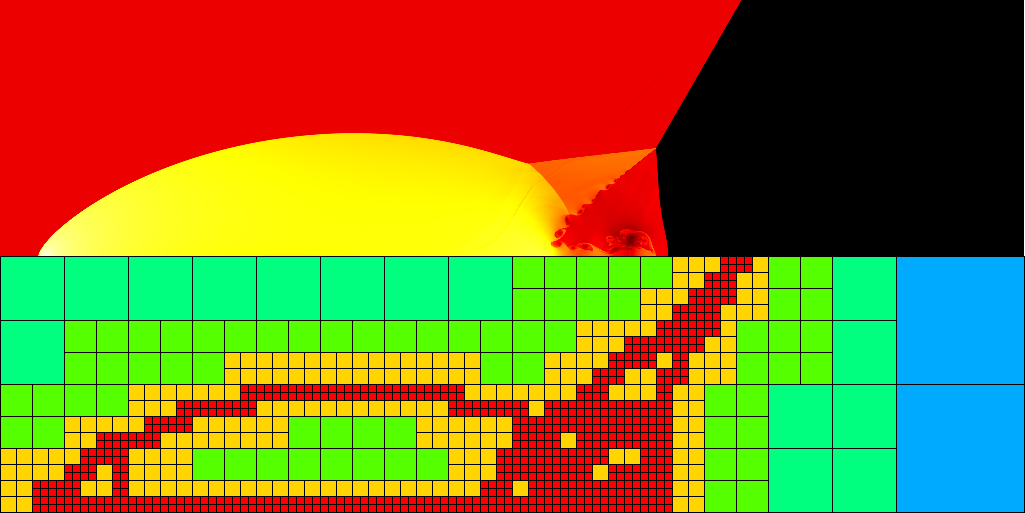
\includegraphics[width=4.0in]{Images/DoubleMachAmr/doublemach-0200.png}
%  % \ANIMATEGRAPHICS{width=4.5in}{20}{Images/DoubleMachAmr/doublemach-}{0000}{0307}
%  
%  
%  %    Boundary
%  %----------------------------------------------------------------------
%  
 \begin{frame}[fragile] 
 \secframetitle{\ssDoubleMach}
 \framesubtitle{\group{Boundary} conditions}
\footnotesize
\begin{semiverbatim}
 \group{Boundary} \{
    \variable{list} = [
            \valuetext{"OUT"},
            \valuetext{"REFLECT"},
            \valuetext{"DENSITY"},
            \valuetext{"VELOCITY_X"},
            \valuetext{"VELOCITY_Y"},
            \valuetext{"TOTAL_ENERGY}"
          ];
\}
\end{semiverbatim}
\end{frame}

%----------------------------------------------------------------------

 \begin{frame}[fragile] 
 \secframetitle{\ssDoubleMach}
 \framesubtitle{\group{Boundary} conditions: outflow and reflecting}
\footnotesize
\begin{semiverbatim}
 \group{Boundary} \{
    \subgroup{OUT} \{
       \variable{type} = \valuetext{"outflow"};
       \variable{mask} = [ (\variable{x} >= \valuetext{4.0}) || 
                (\variable{y} >= \valuetext{1.0} && (\variable{x} >= \valuetext{0.744017} + \valuetext{11.547}* \variable{t}))];
    \};
    \subgroup{REFLECT} \{
       \variable{type} = \valuetext{"reflecting"};
       \variable{axis} = \valuetext{"y"};
       \variable{face} = \valuetext{"lower"};
       \variable{mask} = (\variable{x} >= \valuetext{0.166667});
    \};
\} 
\end{semiverbatim}
\end{frame}

%----------------------------------------------------------------------

 \begin{frame}[fragile] 
 \secframetitle{\ssDoubleMach}
 \framesubtitle{\group{Boundary} conditions: \code{density}}
\footnotesize
\begin{semiverbatim}
\group{Boundary} \{
    \subgroup{DENSITY} \{
       \variable{type} = \valuetext{"inflow"};
       \variable{field_list} = \valuetext{"density"};
       \variable{value} = [ \valuetext{8.0}, 
                  ( (\variable{x} <= \valuetext{0.166667}) && (\variable{y} <= \valuetext{0.0}) ) ||
                    (\variable{x} <= \valuetext{0.0}) ||
                   ((\variable{x} <= \valuetext{0.744017} + \valuetext{11.547}*\variable{t)} && (\variable{y} >= \valuetext{1.0}))
               ];
    \};
\} 
\end{semiverbatim}
\end{frame}

%----------------------------------------------------------------------

 \begin{frame}[fragile] 
 \secframetitle{\ssDoubleMach}
 \framesubtitle{\group{Boundary} conditions: \code{velocity\_x}}
\footnotesize
\begin{semiverbatim}
\group{Boundary} \{
    \subgroup{VELOCITY_X} \{
       \variable{type} = \valuetext{"inflow"};
       \variable{field_list} = \valuetext{"velocity_x"};
       \variable{value} = [ \valuetext{8.25}*\valuetext{0.8660253},
                  ( (\variable{x} <= \valuetext{0.166667}) && (\variable{y} <= \valuetext{0.0}) ) ||
                    (\variable{x} <= \valuetext{0.0}) ||
                   ((\variable{x} <= \valuetext{0.744017} + \valuetext{11.547}*\variable{t)} && (\variable{y} >= \valuetext{1.0}))
               ];
    \};
\}
\end{semiverbatim}
\end{frame}

%----------------------------------------------------------------------

 \begin{frame}[fragile] 
 \secframetitle{\ssDoubleMach}
 \framesubtitle{\group{Boundary} conditions: \code{velocity\_y}}
\footnotesize
\begin{semiverbatim}
\group{Boundary} \{
    \subgroup{VELOCITY_Y} \{
       \variable{type} = \valuetext{"inflow"};
       \variable{field_list} = \valuetext{"velocity_y"};
       \variable{value} = [ -\valuetext{8.25}*\valuetext{0.5},
                  ( (\variable{x} <= \valuetext{0.166667}) && (\variable{y} <= \valuetext{0.0}) ) ||
                    (\variable{x} <= \valuetext{0.0}) ||
                   ((\variable{x} <= \valuetext{0.744017} + \valuetext{11.547}*\variable{t}) && (\variable{y} >= \valuetext{1.0}))
               ];
    \};
\}
\end{semiverbatim}
\end{frame}

%----------------------------------------------------------------------

 \begin{frame}[fragile] 
 \secframetitle{\ssDoubleMach}
 \framesubtitle{\group{Boundary} conditions: \code{total\_energy}}
\footnotesize
\begin{semiverbatim}
\group{Boundary} \{
    \subgroup{TOTAL_ENERGY} \{
       \variable{type} = \valuetext{"inflow"};
       \variable{field_list} = \valuetext{"total_energy"};
       \variable{value} = [ \valuetext{116.5} / (\valuetext{0.4} * \valuetext{8.0}) + \valuetext{34.03125},
                  ( (\variable{x} <= \valuetext{0.166667}) && (\variable{y} <= \valuetext{0.0}) ) ||
                    (\variable{x} <= \valuetext{0.0}) ||
                   ((\variable{x} <= \valuetext{0.744017} + \valuetext{11.547}*\variable{t)} && (\variable{y} >= \valuetext{1.0}))
               ];
    \};
\}
\end{semiverbatim}
\end{frame}

%----------------------------------------------------------------------

 \begin{frame}[fragile] 
 \secframetitle{\ssDoubleMach}
 \framesubtitle{Discretization: \group{Mesh} (forest) and \group{Adapt} (octrees)}
\footnotesize
%    Stopping
% \end{itemize}


\begin{semiverbatim}
\group{Mesh} \{
   \variable{root_rank} = \valuetext{2};
   \variable{root_size} = [\valuetext{96},\valuetext{24}];
   \variable{root_blocks} = [\valuetext{4},\valuetext{1}]; \comment{\# $24^2$ block size}
\}
\group{Adapt} \{
   \variable{max_level} = \valuetext{5}; 
   \variable{list} = [\valuetext{"SLOPE"}];
   \subgroup{SLOPE} \{
      \variable{type} = \valuetext{"slope"};
      \variable{field_list} = [\valuetext{"density"}];
      \variable{min_refine}  = \valuetext{5.0};
      \variable{max_coarsen} = \valuetext{2.0};
   \}
\}
\end{semiverbatim}
\end{frame}

%----------------------------------------------------------------------

 \begin{frame}[fragile] 
 \secframetitle{\ssDoubleMach}
 \framesubtitle{\group{Field} parameters}
\footnotesize
% 
% 
\begin{semiverbatim}
\group{Field} \{
   \variable{gamma} = \valuetext{1.4};
   \variable{list} = [
      \valuetext{"density"},        
      \valuetext{"velocity_x"},
      \valuetext{"velocity_y"},
      \valuetext{"total_energy"},
      \valuetext{"internal_energy"},
      \valuetext{"pressure"} ];
   \variable{ghost_depth} = \valuetext{4}; \comment{\# currently required by interpolation}
   \variable{courant}   = \valuetext{0.8};
\}
\end{semiverbatim}
\end{frame}

%----------------------------------------------------------------------

 \begin{frame}[fragile] 
 \secframetitle{\ssDoubleMach}
 \framesubtitle{\group{Method} parameters}
\footnotesize
\begin{semiverbatim}
\group{Method} \{
   \variable{list} = [\valuetext{"ppm"}];

   \subgroup{ppm} \{
      \variable{diffusion}   = \valuetext{true};
      \variable{flattening}  = \valuetext{3};
      \variable{steepening}  = \valuetext{true};
      \variable{dual_energy} = \valuetext{false};
  \}
\}
\end{semiverbatim}
\end{frame}

%----------------------------------------------------------------------

 \begin{frame}[fragile] 
 \secframetitle{\ssDoubleMach}
 \framesubtitle{\group{Output} parameters}
%\footnotesize
We wish to output
\begin{itemize}
\item HDF5 files of all data
\item density as an image
\item mesh refinement as an image
\end{itemize}

\begin{semiverbatim}
\group{Output} \{ 
   \variable{list} = [\valuetext{"hdf5"},\valuetext{"de_image"},\valuetext{"mesh_image"}];
\}
\end{semiverbatim}
\end{frame}

%----------------------------------------------------------------------

 \begin{frame}[fragile] 
 \secframetitle{\ssDoubleMach}
 \framesubtitle{\group{Output} data as HDF5}
\footnotesize
\begin{semiverbatim}
\group{Output} \{ 
   \subgroup{hdf5} \{
      \variable{type} = \valuetext{"data"};
      \variable{name} = [\valuetext{"doublemach-p%02d-c%04d.h5"}, \valuetext{"proc"},\valuetext{"count"}]; 
      \keyword{include} \valuetext{"input/schedule_cycle_25.incl"}
   \};
\}
\end{semiverbatim}
\end{frame}

%----------------------------------------------------------------------

 \begin{frame}[fragile] 
 \secframetitle{\ssDoubleMach}
 \framesubtitle{\group{Output} image of density}
\footnotesize
\begin{semiverbatim}
\group{Output} \{ 
   \subgroup{de_image} \{
      \variable{type} = \valuetext{"image"};
      \variable{name} = [\valuetext{"doublemach-de-%04d.png"}, \valuetext{"count"}]; 
      \variable{field_list} = [\valuetext{"density"}];
      \variable{image_size} = [\valuetext{1024},\valuetext{256}];
      \keyword{include} \valuetext{"input/schedule_cycle_25.incl"}
      \keyword{include} \valuetext{"input/colormap_blackbody.incl"}
   \};
\}
\end{semiverbatim}
\end{frame}

%----------------------------------------------------------------------

 \begin{frame}[fragile] 
 \secframetitle{\ssDoubleMach}
 \framesubtitle{\group{Output} image of mesh hierarchy}
\footnotesize

\begin{semiverbatim}
\group{Output} \{ 
    \subgroup{mesh_image} \{
        \variable{type}     = \valuetext{"image"};
        \variable{name} = [\valuetext{"doublemach-mesh-%04d.png"}, \valuetext{"count"}];
        \variable{image_type}  = \valuetext{"mesh"};
        \variable{image_reduce_type} = \valuetext{"max"};
        \variable{image_size} = [\valuetext{1025},\valuetext{257}];
        \keyword{include} \valuetext{"input/schedule_cycle_25.incl"}
        \variable{image_specify_bounds} = \valuetext{true};
        \variable{image_min} = \valuetext{0.0};
        \variable{image_max} = \valuetext{6.0};
        \keyword{include} \valuetext{"input/colormap_rainbow.incl"}
      \};
\}
\end{semiverbatim}
\end{frame}

%----------------------------------------------------------------------

\begin{frame}[fragile]
\secframetitle{\ssDoubleMach}
\footnotesize
\begin{center}
\ANIMATEGRAPHICS{width=4.0in}{20}{Images/DoubleMachAmr/doublemach-0}{000}{272}
\end{center}
\end{frame}

 % Case study: Double Mach Reflection
%======================================================================
\NEWSEC
%======================================================================

\subsection{\ssParamActivity}

\begin{frame}[fragile,label=ss-param-activity] 
\secframetitle{\ssParamActivity}
\bluebf{Try the following problem (or make up your own!):}
  \begin{enumerate}
  \item run \code{enzo-P} with \code{input/test\_heat.in} (heat equation)
  \item copy test\_heat.in to test\_heat-unstable.in
  \item edit and rerun with the following changes:
    \begin{itemize}
    \item courant condition of 1.1
    \item output every 10 cycles instead of every 100
    \item stopping criteria of cycle = 100 instead of 1000
    \item output file names e.g.~\code{"heat-unstable-0030.png"} for cycle 30
    \end{itemize}
  \item view generated PNG image files
  \end{enumerate}
\footnotesize
\bluebf{Other things to try}:
  \begin{itemize}
\item What happens if you try running \code{test\_heat.in} with more than 8 processors?
\item What can you do to run on 16 processors?
\item What happens if you change \code{Adapt:max\_level} to 5.0?
\item What happens if you remove the semicolon after \code{temp \{\ldots \}\redcode{;}}?
  \end{itemize}
\end{frame}

 % Case study: Double Mach Reflection
%======================================================================
\NEWSEC
%======================================================================

\subsection{\ssParametersSummary}

%----------------------------------------------------------------------

\begin{frame}[fragile,label=ss-parameters-summary] 
\secframetitle{\ssParametersSummary}
\begin{itemize}
\item Enzo-P / Cello uses a structured parameter file format
\item \parameter{Parameters} are organized into \group{Groups} and \subgroup{subgroups}
\item Suggested procedure for writing parameter files:
\begin{enumerate}
\item Problem definition
\begin{itemize}
\item \group{Domain}, \group{Initial}, \group{Boundary}, \group{Stopping}
\end{itemize}
\item Discretization
\begin{itemize}
\item \group{Mesh}, \group{Adapt}, \group{Field}, \group{Particle}
\end{itemize}
\item Parallel computation
\begin{itemize}
\item \group{Method}, \group{Solver}
\end{itemize}
\item Output
\begin{itemize}
\item \group{Output}
\end{itemize}
\end{enumerate}
\item Parameters are documented at \\ \greentext{\url{http://cello-project.org} / \framebox{Documentation}}
\end{itemize}
\vfill
\centerline{$\qed$}
\end{frame}


% %======================================================================
\NEWSEC
%======================================================================

\subsection{\ssParamProblem}

%======================================================================

\subsection{\ssParamProblem}

\begin{frame}[fragile,label=ss-param-problem] 
\secframetitle{\ssParamProblem}
\framesubtitle{\bluecode{Domain}, \bluecode{Boundary}, \bluecode{Initial}, and \bluecode{Stopping}}

 \newcommand{\DUspan}[2]{\bluetext{#2}}

\footnotesize

\only<1>{\begin{quote}\begin{description}
\item[{Parameter}] \leavevmode
\DUspan{p}{Domain} : \DUspan{p}{lower}
\item[{Summary}] \leavevmode
\DUspan{s}{Lower domain extent}
\item[{Type}] \leavevmode
\DUspan{t}{list} ( \DUspan{t}{float} )
\item[{Default}] \leavevmode
\DUspan{d}{{[}0.0, 0.0, 0.0{]}}
\item[{Scope}] \leavevmode
Cello
\end{description}\end{quote}
%
\DUspan{e}{Lower extent of the computational domain,} {[}x$_{\text{min}}${]}, {[} x$_{\text{min}}$, y$_{\text{min}}${]}, \DUspan{e}{or} {[} x$_{\text{min}}$, y$_{\text{min}}$, z$_{\text{min}}${]}.}

\only<2>{\begin{quote}\begin{description}
\item[{Parameter}] \leavevmode
\DUspan{p}{Domain} : \DUspan{p}{upper}
\item[{Summary}] \leavevmode
\DUspan{s}{Upper domain extent}
\item[{Type}] \leavevmode
\DUspan{t}{list} ( \DUspan{t}{float} )
\item[{Default}] \leavevmode
\DUspan{d}{{[}1.0, 1.0, 1.0{]}}
\item[{Scope}] \leavevmode
Cello
\end{description}\end{quote}
%
\DUspan{e}{Upper extent of the computational domain,} {[}x$_{\text{max}}${]}, {[} x$_{\text{max}}$, y$_{\text{max}}${]}, \DUspan{e}{or} {[} x$_{\text{max}}$, y$_{\text{max}}$, z$_{\text{max}}${]}.}

    
%    Boundary : list
%    Boundary : <condition> : type
%    Boundary : <condition> : axis
%    Boundary : <condition> : face
%    Boundary : <condition> : mask
%    Boundary : <condition> : value
%    Boundary : <condition> : field_list

%    Initial : cycle
%    Initial : type
%    Initial : time
%    Initial : <field> : value
%    Initial : sedov : array
%    Initial : sedov : radius_relative
%    Initial : sedov : pressure_in
%    Initial : sedov : pressure_out
%    Initial : sedov : density
%    Initial : turbulence : density
%    Initial : turbulence : pressure
%    Initial : turbulence : temperature

%    Stopping : cycle
%    Stopping : time
%    Stopping : interval

\end{frame}

 % What parameters are available for defining problems?
%%======================================================================
\NEWSEC
%======================================================================

\subsection{\ssParamRefine}

\begin{frame}[fragile,label=ss-param-refine] 
\secframetitle{\ssParamRefine}
\framesubtitle{\yellowcode{Adapt} and \yellowcode{Mesh} parameter groups}

\begin{verbatim}
    Adapt : interval
    Adapt : max_level
    Adapt : list
    Adapt : <criterion> : field_list
    Adapt : <criterion> : level_exponent
    Adapt : <criterion> : max_coarsen
    Adapt : <criterion> : min_refine
    Adapt : <criterion> : output
    Adapt : <criterion> : type
\end{verbatim}

\begin{verbatim}
    Mesh : root_blocks
    Mesh : root_rank
    Mesh : root_size
\end{verbatim}

\end{frame}

 % What parameters are available for controling mesh refinement?
%%======================================================================
\NEWSEC
%======================================================================

\subsection{\ssParamData}

\begin{frame}[fragile,label=ss-param-data] 
\secframetitle{\ssParamData}
\framesubtitle{\yellowcode{Field} and \yellowcode{Group} parameter groups}

\begin{verbatim}    
    Field : list
    Field : gamma
    Field : alignment
    Field : <field> : centering
    Field : <field> : group_list
    Field : ghost_depth
    Field : padding
    Field : precision
    Field : prolong
    Field : restrict
    Field : interpolation_method
\end{verbatim}
    
\begin{verbatim}    
    Group : list
    Group : <group> : field_list
\end{verbatim}
    
\end{frame}

 % What parameters are available for defining data structures?
%%======================================================================
\NEWSEC
%======================================================================

\subsection{\ssParamMethod}

\begin{frame}[fragile,label=ss-param-method] 
\secframetitle{\ssParamMethod}
\framesubtitle{\yellowcode{Method} parameter groups}

\begin{verbatim}
    Method : list
\end{verbatim}

\begin{verbatim}
    Method : cosmology
    Method : cosmology : comoving_box_size
    Method : cosmology : hubble_constant_now
    Method : cosmology : initial_redshift
    Method : cosmology : max_expansion_rate
    Method : cosmology : omega_lamda_now
    Method : cosmology : omega_matter_now
\end{verbatim}

\begin{verbatim}
    Method : grackle : density_units
    Method : grackle : length_units
    Method : grackle : time_units
    Method : grackle : a_units
    Method : grackle : gamma
    Method : grackle : with_radiative_cooling
    Method : grackle : primordial_chemistry
    Method : grackle : metal_cooling
    Method : grackle : h2_on_dust
    Method : grackle : cmb_temperature_floor
    Method : grackle : data_file
    Method : grackle : three_body_rate
    Method : grackle : cie_cooling
    Method : grackle : h2_optical_depth_approximation
    Method : grackle : photoelectric_heating
    Method : grackle : photoelectric_heating_rate
    Method : grackle : UVbackground
    Method : grackle : UVbackground_redshift_on
    Method : grackle : UVbackground_redshift_off
    Method : grackle : UVbackground_redshift_fullon
    Method : grackle : UVbackground_redshift_drop
    Method : grackle : Compton_xray_heating
    Method : grackle : LWbackground_intensity
    Method : grackle : LWbackground_sawtooth_suppression
    Method : grackle : HydrogenFractionByMass
    Method : grackle : DeuteriumToHydrogenRatio
    Method : grackle : SolarMetalFractionByMass
    Method : grackle : NumberOfTemperatureBins
    Method : grackle : ih2co
    Method : grackle : ipiht
    Method : grackle : TemperatureStart
    Method : grackle : TemperatureEnd
    Method : grackle : comp_xray
    Method : grackle : temp_xray
    Method : grackle : CaseBRecombination
    Method : grackle : NumberOfDustTemperatureBins
    Method : grackle : DustTemperatureStart
    Method : grackle : DustTemperatureEnd
    Method : grackle : cloudy_electron_fraction_factor
\end{verbatim}

\begin{verbatim}
    Method : ppm : density_floor
    Method : ppm : diffusion
    Method : ppm : dual_energy
    Method : ppm : dual_energy_eta_1
    Method : ppm : dual_energy_eta_2
    Method : ppm : flattening
    Method : ppm : minimum_pressure_support_parameter
    Method : ppm : number_density_floor
    Method : ppm : pressure_floor
    Method : ppm : pressure_free
    Method : ppm : steepening
    Method : ppm : temperature_floor
    Method : ppm : use_minimum_pressure_support
\end{verbatim}

\begin{verbatim}
    Method : turbulence : edot
    Method : turbulence : mach_number
\end{verbatim}
\end{frame}

 % What parameters are available for specifying numerical methods?
%%======================================================================
\NEWSEC
%======================================================================

\subsection{\ssParamIo}

\begin{frame}[fragile,label=ss-param-io] 
\secframetitle{\ssParamIo}
\framesubtitle{\yellowcode{Output} parameter group}

\begin{verbatim}
    Output : list
    Output : <file_set> : axis
    Output : <file_set> : colormap
    Output : <file_set> : colormap_alpha
    Output : <file_set> : field_list
    Output : <file_set> : name
    Output : <file_set> : dir
    Output : <file_set> : stride
    Output : <file_set> : type
    Output : <file_set> : image_min
    Output : <file_set> : image_max
    Output : <file_set> : image_specify_bounds
    Output : <file_set> : image_ghost
    Output : <file_set> : image_reduce_type
    Output : <file_set> : image_face_rank
    Output : <file_set> : image_size
    Output : <file_set> : image_log
    Output : <file_set> : image_type
    Output : <file_set> : image_block_size
    Output : <file_set> : image_mesh_color
    Output : <file_set> : schedule : var
    Output : <file_set> : schedule : value
    Output : <file_set> : schedule : start
    Output : <file_set> : schedule : stop
    Output : <file_set> : schedule : step
\end{verbatim}

\end{frame}

 % What parameters are available for controling I/O?
%%======================================================================
\NEWSEC
%======================================================================

\subsection{\ssParamOther}

\begin{frame}[fragile,label=ss-param-other] 
\secframetitle{\ssParamOther}
\framesubtitle{\yellowcode{Balance},
               \yellowcode{Memory},
               \yellowcode{Monitor},
               \yellowcode{Performance},
               \yellowcode{Restart},
               and \yellowcode{Test} parameter groups}


\begin{verbatim}
    Balance : interval
\end{verbatim}

    method specified when running: charmrun p4 balancer
    list load balancing methods available in Charm++ and status
    include 

\begin{verbatim}
    Memory : active
\end{verbatim}

\begin{verbatim}
    Monitor : debug
\end{verbatim}

\begin{verbatim}
    Performance : name
    Performance : stride
    Performance : papi : counters
\end{verbatim}

\begin{verbatim}
    Restart : file
\end{verbatim}

\begin{verbatim}
    Testing : cycle_final
    Testing : time_final
    Testing : time_tolerance
\end{verbatim}

\end{frame}

 % What other parameters are available?


  %======================================================================
\NEWMOD
%======================================================================

\section{\sCharm}

%----------------------------------------------------------------------

\logo{\hfill\hyperlink{outline<1>}{\icon}}

\begin{frame}[fragile,label=s-charm] 
\modframetitle{\sCharm}
\small
\begin{center}
\begin{minipage}{3.25in}
\begin{enumerate}
\item \hyperlink{ss-charm<1>}      {\BUTTON {\ssCharm}}
\item \hyperlink{ss-charm-code<1>} {\BUTTON {\ssCharmCode}}
\item \hyperlink{ss-charm-cello<1>}{\BUTTON {\ssCharmCello}}
\item \hyperlink{ss-charm-pup<1>}{\BUTTON {\ssCharmPup}}
\item \hyperlink{ss-charm-summary<1>}{\BUTTON {\ssCharmSummary}}
\end{enumerate}
\end{minipage}
\end{center}
\end{frame}

\logo{\hfill\hyperlink{s-charm<1>}{\icon}}

%======================================================================
\NEWSEC
%======================================================================

\subsection{\ssCharm}

\begin{frame}[fragile,label=ss-charm] 
\secframetitle{\ssCharm}
%--------------------------------------------------
\framesubtitle{MPI parallel programs: passing messages between processes}
%--------------------------------------------------
\begin{minipage}[t]{1.75in}
\begin{center}
\begin{minipage}{1.50in}
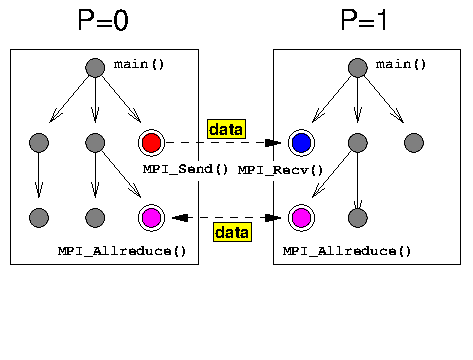
\includegraphics[width=1.50in]{mpi.pdf}\\
\vspace{-0.5in}
\centerline{\scriptsize\textbf{An MPI parallel program}}
\end{minipage}\\ \ \\
%\begin{minipage}{1.25in}
%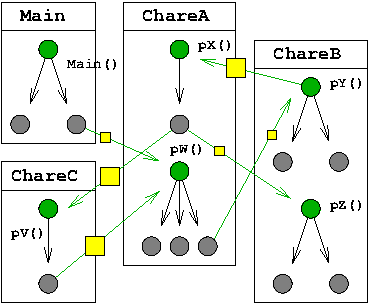
\includegraphics[width=1.25in]{charm.pdf}
%\ \\
%\centerline{\scriptsize\textbf{A Charm\pp\ parallel program}}
%\end{minipage}
\end{center}
\end{minipage} \ 
\begin{minipage}[t]{2.50in}
\vspace{-0.6in}
\begin{itemize}
\item MPI program
  \begin{itemize}
  \item decomposed by \blueit{processes}
  \item calls MPI library
  \item communicate / synchronize
  \end{itemize}
\ \\ \pause
\item MPI runtime system
  \begin{itemize}
  \item sends data between processes
  \item synchronizes between processes
  \end{itemize} \pause
\item Additional features
\begin{itemize}
\item MPI-2: Parallel I/O, remote DMA,
one-sided communication
\item MPI-3: fault-tolerance, hybrid programming, persistence
\end{itemize}
\end{itemize}
\end{minipage}
\end{frame}

\begin{frame}[fragile]
\secframetitle{\ssCharm}
%--------------------------------------------------
\framesubtitle{\charm\ parallel programs: collections of asynchronously-interacting objects}
%--------------------------------------------------
\begin{minipage}[t]{1.75in}
\begin{center}
\begin{minipage}{1.25in}
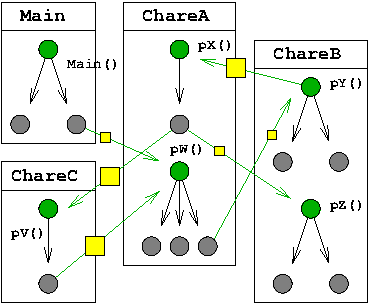
\includegraphics[width=1.25in]{charm.pdf}
\ \\
\centerline{\scriptsize\textbf{A Charm\pp\ parallel program}}
\end{minipage}\\ \ \\
\ \\
\hrule
\ \\
\begin{minipage}{1.50in}
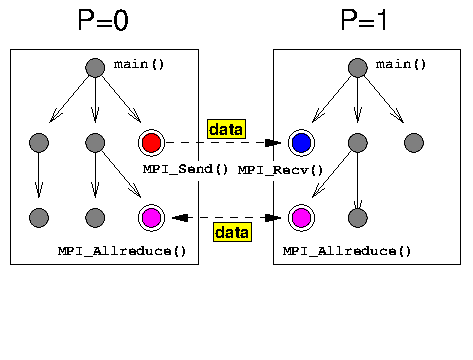
\includegraphics[width=1.50in]{mpi.pdf}\\
\vspace{-0.5in}
\centerline{\scriptsize{An MPI parallel program}}
\end{minipage}
\end{center}
\end{minipage} \ 
\begin{minipage}[t]{2.50in}
\vspace{-0.70in}
\begin{itemize}
\item \charm\ program
  \begin{itemize}
  \item Decomposed by \blueit{objects}
  \item \charm\ objects called \blueit{chares}
  \item invoke \blueit{entry methods}
  \item \blueit{asynchronous}
  \item communicate via \blueit{messages}
  \end{itemize}
\ \\ \pause
\item \charm\ runtime system
  \begin{itemize}
  \item maps chares to processors
  \item schedules entry methods
  \item migrates chares to load balance
  \end{itemize} \pause
\item Additional features
\begin{itemize}
\item checkpoint/restart
\item dynamic load balancing
\item fault-tolerance
\end{itemize}
\end{itemize}
\end{minipage}
\end{frame}

\begin{frame}[fragile] 
\secframetitle{\ssCharm}
%--------------------------------------------------
%\framesubtitle{Anatomy of a simple Charm program}
%--------------------------------------------------

%     Look at simple HelloWorld Charm++ code
%        Control files
%          *.ci
         
%        Main
%        chare Group
%           one class created per process
% 	  indexed by ip
%        Chare Array
%           at least one class created per process

\begin{itemize}
\item C++ program with ``extra features''
\item Defined using ``\bluecode{.ci}'' control files: 
\begin{itemize}
\item which classes are chares
\item which methods are entry methods
\item declare message objects
\item declare global ``\code{readonly}'' variables
\end{itemize}
\item compiled using \bluecode{charmc}
\item generates \bluecode{.decl.h} and \bluecode{.def.h} from \bluecode{.ci}
\begin{itemize}
\item ``hooks'' program to \charm\ runtime
\item \bluecode{.decl.h} declarations
\item \bluecode{.def.h}: include definitions
\end{itemize}
\item Run executable using \bluecode{charmrun}
\end{itemize}
\end{frame}

% ----------------------------------------------------------------------
\begin{frame}[fragile] 
\secframetitle{\ssCharm}
\framesubtitle{Chare objects}
\framesubtitle{Chares are concurrent objects}
\begin{itemize}
\item Chares are C++ objects
\item Inherit from \charm\ base class
\footnotesize
\begin{semiverbatim}
#\bluetext{include} \orangetext{"foo.decl.h"}
\bluetext{class} \greentext{Foo} : \bluetext{public} \redtext{CBase_}\greentext{Foo} \{
   \bluetext{Foo} (\greentext{int} \orangetext{n});
   \greentext{void} \bluetext{p_receive_data} (\greentext{int} \orangetext{n}, \greentext{double} * \orangetext{a});
   \greentext{void} \bluetext{print_results} ();
\};
#\bluetext{include} \orangetext{"foo.def.h"}
\end{semiverbatim}
\normalsize
\item Chares and entry methods declared in \code{.ci} control file
\footnotesize
\begin{semiverbatim}
\greentext{module foo} \{
   \greentext{chare} \bluetext{Foo} \{
      \greentext{entry} \bluetext{Foo} (\greentext{int} \orangetext{n});
      \greentext{entry void} \bluetext{p_receive_data} (\greentext{int} \orangetext{n}, \greentext{double} \orangetext{a}[\orangetext{n}]);
   \};
\}
\end{semiverbatim}
\end{itemize}
%\normalsize
%\item \redcode{CBase\_}\greencode{Foo} declared in \bluecode{.decl.h} file
%\item \redcode{CBase\_}\greencode{Foo} defined in \bluecode{.def.h} file
%\end{itemize}
\end{frame}

% ----------------------------------------------------------------------
\begin{frame}[fragile] 
\secframetitle{\ssCharm}
\framesubtitle{\charm\ control files}

\bluebf{Example control file: \bluecode{hello.ci}}

 \begin{semiverbatim}
    \bluecode{mainmodule} \greencode{hello} \{
       \bluecode{readonly} \greencode{CProxy_Main mainProxy};
       \bluecode{mainchare} \greencode{main} \{
          \bluecode{entry} \greencode{main}(\bluecode{CkArgMsg}*);
       \};
    \};
\end{semiverbatim}
\vspace{-0.2in}
\begin{itemize}
\item \charm\ programs start in a \blueit{mainchare}
\item Other chares created dynamically using \bluecode{ckNew()}
\begin{itemize}
\item new chare may reside remotely
\item \code{ckNew()} returns \blueit{proxy} to chare
\item entry methods called via \bluetext{proxy}
\end{itemize}

\end{itemize}
\end{frame}

\begin{frame}[fragile] 
\secframetitle{\ssCharm}
\framesubtitle{\charm\ collections of chares}
\vspace{-0.2in}
\begin{center}
\begin{minipage}{4in}
\begin{minipage}{1.5in}
\bluebf{Chare Arrays}
\end{minipage} \ 
\begin{minipage}{2in}

\includegraphics[width=2.0in]{chare-array.pdf}
\end{minipage}
\vspace{0.1in}
  \begin{itemize}
  \item \bluetext{distributed array of chares}
  \item \bluetext{migratable elements}
  \item \bluetext{flexible indexing}
  \end{itemize}
\vspace{0.2in}
\begin{minipage}{1.5in}
\redbf{Chare Groups}
\end{minipage} \ 
\begin{minipage}{2in}
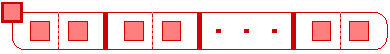
\includegraphics[width=2.0in]{chare-group.pdf}
\end{minipage}
  \begin{itemize}
\setbeamercolor*{item}{fg=red!50!black}
  \item \redtext{one chare per processor (non-migratable)}
  \end{itemize}
\vspace{0.2in}
\begin{minipage}{1.5in}
\greenbf{Chare Nodegroups}
\end{minipage} \ 
\begin{minipage}{2in}
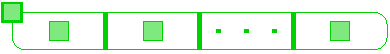
\includegraphics[width=2.0in]{chare-nodegroup.pdf}
\end{minipage}
  \begin{itemize}
\setbeamercolor*{item}{fg=green!50!black}
  \item \greentext{one chare per node (non-migratable)}
  \end{itemize}
\end{minipage}
\end{center}

\end{frame}

 % What is Charm++?
%======================================================================
\NEWSEC
%======================================================================

\subsection{\ssCharmCode}

% \begin{frame}[fragile,label=ss-charm-code] 
% \secframetitle{\ssCharmCode}
% \framesubtitle{Anatomy of a simple Charm program}
% 
% \begin{itemize}
% \item Extra Charm++ control files: .ci
% \begin{itemize}
% \item define chares, entry methods
% \end{itemize}
% \item Rest of Charm++ programs are  C++
% \begin{itemize}
% \item compiled using \bluecode{charmc}
% \item generates .def.h and .decl.h from .ci
% \item include definitions from .def.h
% \item include declarations from .decl.h
% \end{itemize}
% \item Run using \bluecode{charmrun}
% \end{itemize}
% 
% 
% %     Look at simple HelloWorld Charm++ code
%        Control files
%          *.ci
         
%        Main
%        chare Group
%           one class created per process
% 	  indexed by ip
%        Chare Array
%           at least one class created per process



 % How do I write a simple Charm program?
%======================================================================
\NEWSEC
%======================================================================

\subsection{\ssCharmCello}

\begin{frame}[fragile,label=ss-charm-cello] 
% ----------------------------------------------------------------------
\secframetitle{\ssCharmCello}
\begin{itemize}
\item \code{Enzo-P} begins in the \cyancode{mainchare}
\begin{itemize}
\item single chare on root process
\item creates a \redcode{Simulation} chare group
\end{itemize}
\item \redcode{Simulation} stores ``global'' data
\begin{itemize}
\item one \redcode{Simulation} object per physical process
\item creates \bluecode{Block} chare array
\end{itemize}
\item \bluecode{Block}s associated with octree nodes
\begin{itemize}
\item many \bluecode{Block}s per process
\item indexed using bit-coding of location
\end{itemize}
\end{itemize}

\end{frame}

\begin{frame}[fragile] 
% ----------------------------------------------------------------------
\secframetitle{\ssCharmCello}
\begin{center}
\begin{minipage}{1.00in}
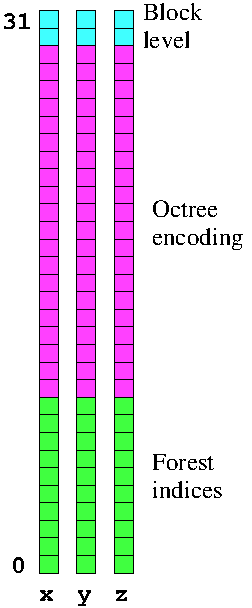
\includegraphics[width=1.0in]{index.pdf}
\end{minipage}
\begin{minipage}{3.25in}
\begin{itemize}
\item User-defined chare array indices supported
\item \cello\ indices for \code{Block} arrays:
\begin{itemize}
\item $3 \times 10 $ bits for \greenit{array indices} 
\item $3 \times 20 $ bits for the \magentait{octree encoding}
\item $6$ bits for the \cyanit{block level}
\end{itemize}
\item Up to $1024^3$ array of octrees
\item Up to $20$ octree levels
\item $-31 \le$ level $\le 31$
\item Block id's use index: e.g. \bluecode{B100:11\_1:01}
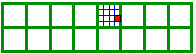
\includegraphics[width=1.2in]{block-index.pdf}
\end{itemize}
\end{minipage}
\end{center}
\end{frame}
%----------------------------------------------------------------------


 % How is Charm++ used in Cello?
%======================================================================
\NEWSEC
%======================================================================

\subsection{\ssCharmPup}

\begin{frame}[fragile,label=ss-charm-pup] 
\secframetitle{\ssCharmPup}
\end{frame}

 % How is Charm++ used in Cello?
%======================================================================
\NEWSEC
%======================================================================

\subsection{\ssCharmSummary}

%----------------------------------------------------------------------

\begin{frame}[fragile,label=ss-charm-summary] 
\secframetitle{\ssCharmSummary}

\vfill
\centerline{$\qed$}
\end{frame}



% 
% CONCEPTS
%  Chare program
%    chare objects
%    Messages
%    Entry Methods
%    Proxies
%  Chare collections
%    chare arrays
%    chare groups
%    chare node groups
%  Charm runtime system
%    Mapping Chare Objects to Physical Processors
%    Load-Balancing Chare Objects
%    Routing of Messages:
%    Checkpointing
%    Fault-Tolerance
%    Dynamic Re-Allocation of Physical Resources
%  A Simple Charm++ Program
%    charmc
%    interface file: ``.ci''
%    charmc generates ``decl.h'' and ``def.h'' files
%    ``hooks'' to programmers application code to runtime system
%  Running a Charm++ program
%    charmrun
%  Where to find more information
%     Charm group is very active and 
%    

  %======================================================================
\NEWMOD
%======================================================================

\section{\sDesign}

%----------------------------------------------------------------------

\logo{\hfill\hyperlink{outline}{\icon}}

\begin{frame}[fragile,label=s-design] 
\modframetitle{\sDesign}
\small
\begin{center}
\begin{minipage}{3.25in}
\begin{enumerate}
\item \hyperlink{ss-oop}   {\ssOop}
\item \hyperlink{ss-components}   {\ssComponents}
\item \hyperlink{ss-classes}   {\ssClasses}
\item \hyperlink{ss-simulation}   {\ssSimulation}
\item \hyperlink{ss-problems}   {\ssProblems}
\item \hyperlink{ss-blocks}   {\ssBlocks}
%\item \hyperlink{ss-data}   {\ssData}
\item \hyperlink{ss-fields}   {\ssFields}
\item \hyperlink{ss-particles}   {\ssParticles}
\item \hyperlink{ss-methods}   {\ssMethods}
\item \hyperlink{ss-initial-boundary}   {\ssInitialBoundary}
\item \hyperlink{ss-refine}   {\ssRefine}
\item \hyperlink{ss-design-summary}   {\ssDesignSummary}
%\item \hyperlink{ss-stopping}   {\ssStopping}
%\item \hyperlink{ss-classes-org}   {\ssClassesOrg}
%\item \hyperlink{ss-data}   {\ssData}
\end{enumerate}
\end{minipage}
\end{center}
\end{frame}

\logo{\hfill\hyperlink{s-design}{\icon}}

%======================================================================
\NEWSEC
%======================================================================

\subsection{\ssOop}

\begin{frame}[fragile,label=ss-oop] 
\secframetitle{\ssOop}
\bluebf{Enzo-P/Cello's design is \blueit{object-oriented}}

\begin{itemize}
\item Package-level design
\begin{itemize}
\item \bluecode{Enzo-P} \bluetext{application} implemented using \greencode{Cello} \greentext{AMR framework}
\item \greencode{Cello} implemented using \redcode{Charm++} \redtext{parallel programming system}
\end{itemize}
\item Component-level design
\begin{itemize}
\item \code{Cello} is decomposed into high-level \greenit{components}
\item Components are comprised of one or more \greenit{classes}
\end{itemize}
\item Source code is organized by package, component, and class
\begin{itemize}
\footnotesize
\item \bluecode{Enzo-P}:
\bluecode{cello-src/src/Enzo/}\blueit{enzo\_<class>}\bluecode{.[ch]pp}
\item \greentext{Cello}:
\greencode{cello-src/src/Cello/}\greenit{<component>\_<class>}\greencode{.[ch]pp}
\end{itemize}
\end{itemize}

\end{frame}

%----------------------------------------------------------------------

%\begin{frame}[fragile] 
%\secframetitle{\ssOop}
%\end{frame}
 % Object-oriented design
%======================================================================
\NEWSEC
%======================================================================

\subsection{\ssComponents}

%----------------------------------------------------------------------

\begin{frame}[fragile,label=ss-components] 
\secframetitle{\ssOop}
\framesubtitle{Cello software components}
\vspace{-0.2in}
\begin{center}
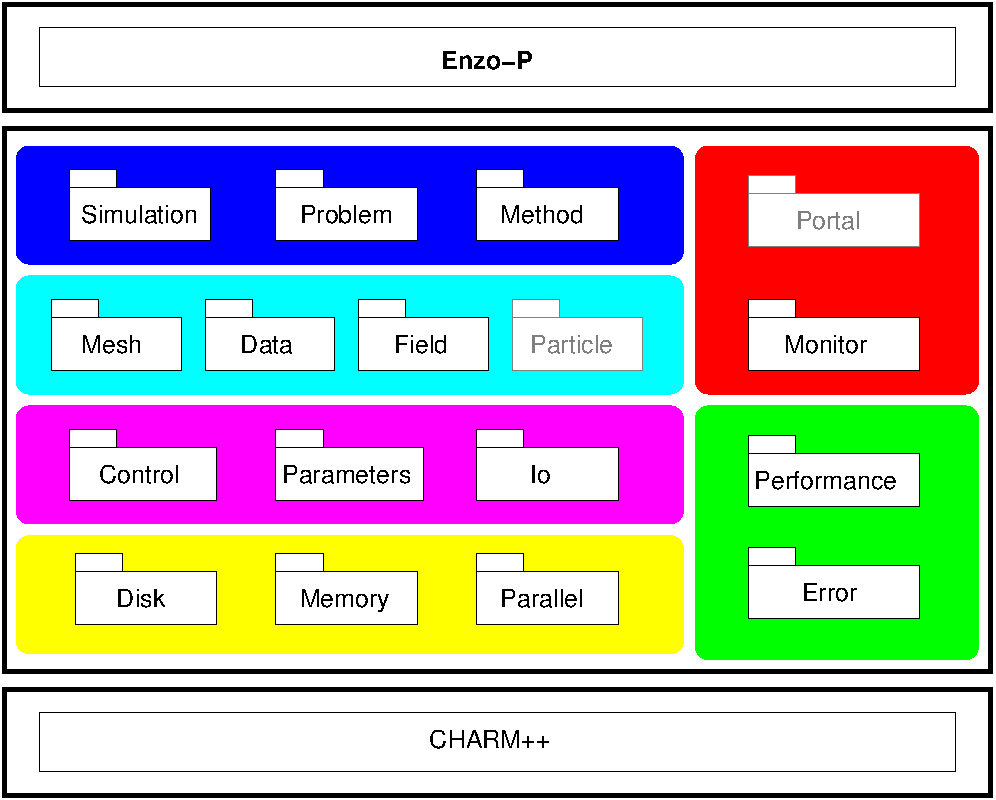
\includegraphics[width=3.0in]{components-1509.pdf}
\end{center}
\end{frame}

%----------------------------------------------------------------------

\begin{frame}[fragile] 
\secframetitle{\ssComponents}
\framesubtitle{Cello software components}
Cello's components are loosely grouped into categories
\begin{center}
\begin{minipage}{3in}
\begin{tabbing}
xxxxxxxxxxxxxxxxxxx\=\kill
\bluetext{High-level}\> \bluetext{Simulation}, \bluetext{Problem}, \bluetext{Method} \\
\cyantext{Data structures}\> \cyantext{Mesh}, \cyantext{Data}, \cyantext{Field}, \cyantext{(Particle)} \\
\magentatext{Middle-level}\> \magentatext{Control}, \magentatext{Parameters}, \magentatext{Io}  \\
\yellowtext{Hardware-interface}\> \yellowtext{Disk}, \yellowtext{Memory}, \yellowtext{Parallel} \\
\redtext{Interface}\> \redtext{Monitor}, \redtext{(Portal)}  \\
\greentext{Cross-cutting}\> \greentext{Performance}, \greentext{Error}
\end{tabbing}
\end{minipage}
\end{center}
\end{frame}

%----------------------------------------------------------------------

\begin{frame}[fragile] 
\secframetitle{\ssComponents}
\framesubtitle{\bluetext{High-level components}}
\bluebf{High-level components define the core classes in Enzo-P/Cello}

\begin{itemize}
\item \bluetext{Simulation}s define and manage computational \bluetext{Problem}s
(\bluecode{Simulation}, \bluecode{EnzoSimulation})
\item A \bluetext{Problem} defines the problem to be solved:
\begin{itemize}
\item numerical methods (\bluecode{EnzoMethodPpm}, etc.)
\item initial conditions (\bluecode{Initial})
\item boundary conditions (\bluecode{Boundary})
\item stopping criteria  (\bluecode{Stopping})
\item output (\bluecode{Output})
\item \textit{etc.}
\end{itemize}
\item A \bluetext{Method} implements a numerical method
\begin{itemize}
\item operates on block \bluetext{Data}
\end{itemize}

\end{itemize}
\end{frame}

%----------------------------------------------------------------------

\begin{frame}[fragile] 
\secframetitle{\ssComponents}
\framesubtitle{\cyantext{Data structure components}}
\cyanbf{Data structure classes define the AMR hierarchy and its data}

\begin{itemize}
\item \cyantext{Mesh} classes represent and operate on an AMR mesh (\cyancode{Hierarchy})
\item \cyantext{Data} classes store data on an AMR \textit{block} (\cyancode{Data}, \cyancode{EnzoData})
\item \cyantext{Field} classes store field data on a block
\begin{itemize}
\item \cyancode{FieldData}: field data on a block
\item \cyancode{FieldDescr}: global description of field data
\end{itemize}
\item \cyantext{Particle} classes will represent particle data on a block
\begin{itemize}
\item \cyancode{ParticleData}: particle data on a block
\item \cyancode{ParticleDescr}: global description of particle data
\end{itemize}
\end{itemize}
\end{frame}

%----------------------------------------------------------------------

\begin{frame}[fragile] 
\secframetitle{\ssComponents}
\framesubtitle{\magentatext{Middle-level components}}
\magentabf{Middle-level component interface high- and low-level classes}

\begin{itemize}
\item \magentatext{Control} handles problem evolution
\begin{itemize}
\item analagous to Enzo's \bluecode{EvolveHierarchy}, \bluecode{EvolveLevel}
\end{itemize}

\item \magentatext{Parameter} classes
\begin{itemize}
\item read parameters from a file (\magentacode{Parameters}) 
\item provide access to parameters (\magentacode{Config}, \magentacode{EnzoConfig})
\end{itemize}
\item \magentatext{Io} classes perform parallel IO
\begin{itemize}
\item \magentacode{OutputData} for writing data files
\item \magentacode{OutputImage} for writing image files
\item \magentacode{Schedule} for defining when to write files
\item \magentacode{IoHierarchy}, \magentacode{IoBlock}, \magentacode{IoFieldData}
interface data structure classes with \yellowtext{Disk} classes
\end{itemize}
\end{itemize}
%  include Control handles the time stepping of Method s to advance the
% problem forward in time, as well as sequencing adaptive mesh
% refinement data structure operations, including remeshing, scheduling
% dynamic load balancing (which will be delegated to Charm++), and
% refreshing ghost zones on Block boundaries. The Parameters component
% serves to read, store, and provide access to parameters defined in an
% input configuration file. To improve usability over Enzo,
% configuration files are more structured, and support floating-point
% and logical expressions to greatly simplify initializing problems with
% complex initial conditions. The Io component serves as a layer to
% coordinate the disk output of data structure components, such as
% Simulation Hierarchy and Field data. It calls the Disk component to
% handle actual file operations.  \end{frame}
\end{frame}

%----------------------------------------------------------------------

\begin{frame}[fragile] 
\secframetitle{\ssComponents}
\framesubtitle{\yellowtext{Hardware-interface components}}
\yellowbf{Hardware-interface components interface to system libraries}

\begin{itemize}
\item \yellowtext{Disk} classes write meta-data and data to files (\yellowcode{FileHdf5})
\item \yellowtext{Memory} tracks dynamic memory allocation
\item \yellowtext{Parallel} provides helper classes for parallelization
\begin{itemize}
\item \yellowcode{ArrayMap}: how to map chare array elements to processes
\item \yellowcode{Sync}: simple counter to ease Charm++ synchronization
\end{itemize}
\end{itemize}
% The lower-level components include Disk, Memory and Parallel. The Disk
% component implements basic disk operations, isolating the specific
% file format from the higher-level Io component. Disk currently
% supports HDF5, and we propose to support the Adaptable IO System
% (ADIOS) in the future to enhance transfer of data to and from other
% HPC software components. The Memory component controls dynamic memory
% allocation and management. Currently Memory handles allocating and
% monitoring heap memory usage; proposed functionality includes
% allocating, deallocating, and transferring data between main memory,
% hardware accelerator (GPU) memory, and many-core coprocessors
% (e.g.~the Intel Xeon Phi). As with the Disk component, this serves to
% isolate lower-level details from higher-level components. The Parallel
% component currently supplies basic access to core rank and core count,
% and is being depreciated.
\end{frame}

%----------------------------------------------------------------------

\begin{frame}[fragile] 
\secframetitle{\ssComponents}
\framesubtitle{\redtext{Interface} and \greentext{Cross-cutting} components}
\redbf{Interface components link Enzo-P / Cello with the outside world}

\begin{itemize}
\item \redtext{Monitor} keeps users informed of application status (\redcode{Monitor})
\item \redtext{(Portal)} will interface with external users / applications
\end{itemize}
\ \\
\ \\

\greenbf{Cross-cutting components are for globally-accessed classes}
\begin{itemize}
\item \greentext{Performance} measures and reports on application performance
\item \greentext{Error} provides basic error-handling support
\end{itemize}
% Interface compenents include Monitor (current) and Portal
% (proposed). The Monitor component controls the user-readable summary
% of progress to stdout, and the proposed Portal component will control
% the interaction of Enzo-P with external applications running
% concurrently, such as inline analysis or real-time visualization. One
% particular such analysis and visualization application is yt, which we
% will use to help drive the design and development of the Portal
% component.  
\end{frame}

%----------------------------------------------------------------------

%\begin{frame}[fragile] 
%\secframetitle{\ssComponents}
%\framesubtitle{: \greentext{Performance}, \greentext{Error}}
% Some Cello components can in principle be called from any software
% layer—these include Performance and Error. The Performance component
% dynamically collects performance data for the running Enzo-P
% simulation, and provides a holistic summary of performance data to the
% user, as well as to software components that can adapt to optimize
% desired performance metrics. Current metrics measured include memory
% usage (via the Memory component), and computation amount and memory
% access amount (via the Performance Application Programming Interface
% (PAPI). Future support will include metrics for monitoring parallel
% communication, dynamic load balancing, and disk usage. The Error
% component will be used to detect, evaluate, and decide what to do
% about software errors; higher-level error detection and recovery will
% be handled by Charm++, which supports both simple checkpoint to disk,
% as well as double in-memory checkpoint with automatic restart.
%\end{frame}


%    include component diagram (update from nsf proposal)
%    Go through each component and describe


%  Sequence diagram
%   Hardware components
%      Disk, Memory

% Mid-level-components

% Data structure components
%     Simulation
%     Hierarchy
%     CommBlock
%     Block
%     field\_block [field\_face]
%     [particle\_block]
%     example code

% Computational components

% Control components

% Cross-cutting components

%    Cello:     src/Cello/<component>\_<Class>.[hc]pp
%    Enzo-P:    src/Enzo/enzo\_<EnzoClass>.[hc]pp
%
%    examples
%
%    include Enzo component 
%
%    Note components are meant to be agile: can and have been redefined


% Top level components of Cello include . 
% 
% 
%Hardware-interface components
% 
%  Interface components
% 
%Cross-cutting components
% 


 % Cello software components
%======================================================================
%\NEWSEC
%======================================================================

%\subsection{\ssClasses}

\begin{frame}[fragile,label=ss-classes] 
\secframetitle{\ssClasses}
\begin{center}
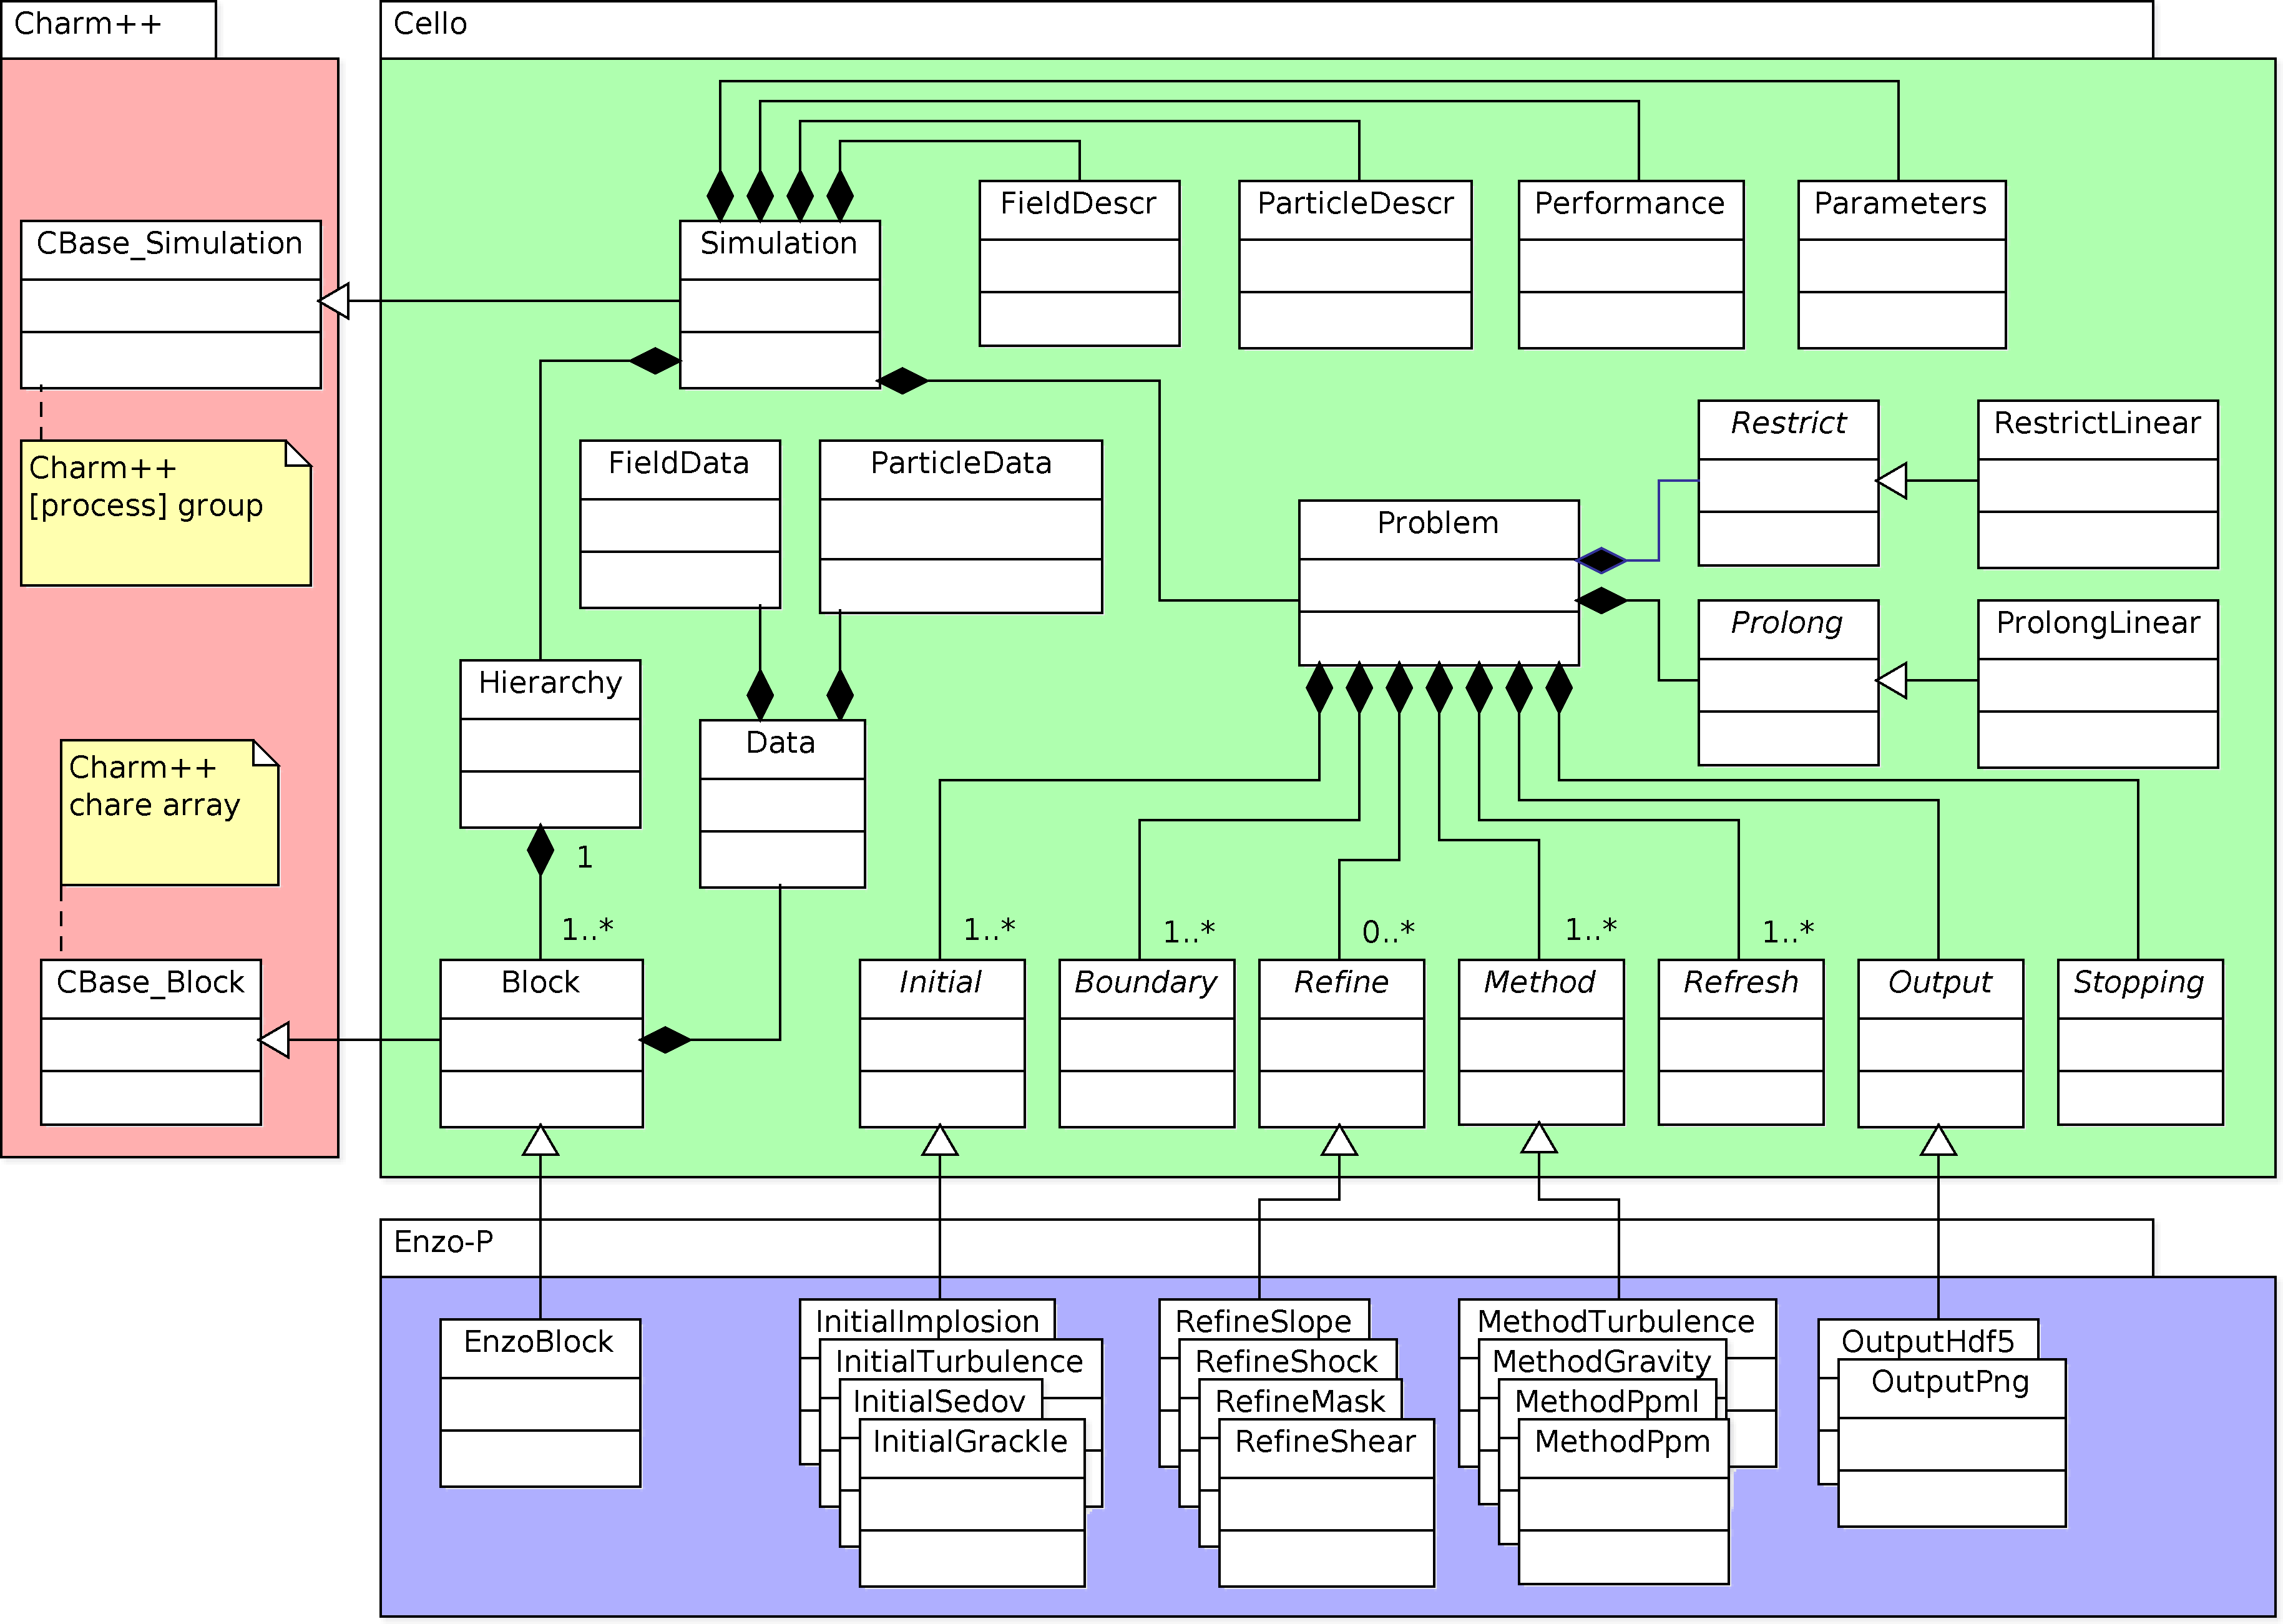
\includegraphics[width=3.5in]{ClassDiagram-color.png}
\end{center}
\end{frame}



 % Enzo-P / Cello classes
%======================================================================
\NEWSEC
%======================================================================

\subsection{\ssSimulation}
\begin{frame}[fragile,label=ss-simulation] 
\secframetitle{\ssSimulation}
\greenbf{\textit{Simulation} classes represents a numerical simulation}

\begin{tabbing}
xxxx\=xxxxxxxxxxxxxx\=\kill
\> \greencode{Problem} \> \redit{A numerical problem} \\
\> \greencode{Config} \> \redit{Parameter values} \\
\> \greencode{Hierarchy} \> \redit{Mesh hierarchy} \\
\> \greencode{Performance} \> \redit{Performance measurements} \\ 
\> \greencode{Monitor} \> \redit{Monitor output} \\ 
\> \greentext{state data} \> \redit{cycle, time, dt, etc.}
\end{tabbing}

\begin{itemize}
  \item Implemented as a \redit{chare group}
    \begin{itemize}
  \item One \bluecode{EnzoSimulation} object per process
    \end{itemize}
  \item Stores simulation ``global'' data
\end{itemize}

\end{frame}

 % Simulation objects
%======================================================================
\NEWSEC
%======================================================================

\subsection{\ssProblems}

\begin{frame}[fragile,label=ss-problems] 
\secframetitle{\ssProblems}
\greenbf{Problem classes represents a numerical problem}

\begin{tabbing}
xxxx\=xxxxxxxxxxxx\=\kill
\> \greencode{Method} \>   \redit{Numerical methods} \\
\> \greencode{Initial} \>  \redit{Initial conditions} \\
\> \greencode{Boundary} \> \redit{Boundary conditions} \\
\> \greencode{Refine} \>   \redit{Mesh refinement criteria} \\
\> \greencode{Stopping} \> \redit{Stopping criteria} \\
\> \greencode{Output} \>   \redit{Disk Output} \\
\> \greencode{Prolong} \>  \redit{Interpolation scheme} \\
\> \greencode{Restrict} \> \redit{Coarsening scheme}
\end{tabbing}
\begin{itemize}
\item  Base class \greencode{Problem} initializes Cello \code{Problem} objects
\item Subclass \bluecode{EnzoProblem} initializes Enzo \code{Problem} objects
\end{itemize}
\end{frame}

 % How are problems represented in Enzo-P/Cello?
%======================================================================
\NEWSEC
%======================================================================

\subsection{\ssBlocks}

\begin{frame}[fragile,label=ss-blocks] 
\secframetitle{\ssBlocks}
\greenbf{Block objects represent blocks in the octree array}

%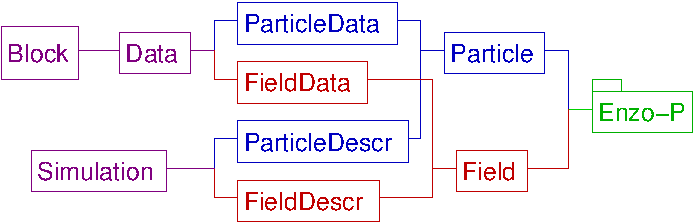
\includegraphics[width=2in]{data-classes.pdf}
\begin{tabbing}
xxxx\=xxxxxxxxxxxxxx\=\kill
\> \greencode{Data} \> \redit{Block data} \\
\> \greencode{Sync} \> \redit{Synchronization counters} \\
\> \greentext{state data} \> \redit{cycle, time, dt, etc.} \\
\> \greentext{face data} \> \redit{neighbor refinement levels} \\
\> \ \ \ \ \greenit{etc.}
\end{tabbing}
\vspace{-0.2in}
\begin{itemize}
\item Implemented as a \redit{chare array}
\item One \bluecode{EnzoBlock} object per octree array node
\end{itemize}

\end{frame}

%----------------------------------------------------------------------

\begin{frame}[fragile,label=ss-blocks] 
\secframetitle{\ssBlocks}
\greenbf{\code{Data} objects contain numerical data associated with \code{Block}s}
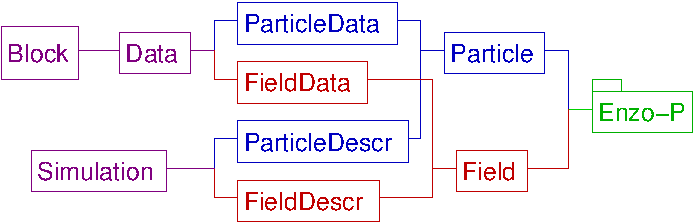
\includegraphics[width=2in]{data-classes.pdf}
\begin{tabbing}
xxxx\=xxxxxxxxxxxxxxxx\=\kill
\> \greencode{FieldBlock} \> \redit{Field (array) block data} \\
\> \greencode{ParticleBlock} \> \redit{Particle block data}
\end{tabbing}
\end{frame}
 % How are blocks represented in Enzo-P/Cello?
%%======================================================================
\NEWSEC
%======================================================================

\subsection{\ssData}

\begin{frame}[fragile,label=ss-data] 
\secframetitle{\ssData}

\end{frame}

 % What data types are available?
%======================================================================
\NEWSEC
%======================================================================

\subsection{\ssFields}

\begin{frame}[fragile,label=ss-fields] 
\secframetitle{\ssFields}
\greenbf{Field classes represent field data on \code{Block}s}
\ \\

\begin{itemize}
\item \greencode{FieldBlock}
\begin{itemize}
\item represents state-independent (intrinsic) data
\item stored in \greencode{Block} \greencode{Data} objects
\item raw arrays
\end{itemize}
\item \greencode{FieldDescr}
\begin{itemize}
\item represents state-dependent (extrinsic) data
\item stored in \greencode{Simulation} object
\item precision, ghost depth, padding, alignment, centering
\end{itemize}
\item \greencode{Field} used to simplify using \greencode{FieldBlock} and \greencode{FieldDescr}
\end{itemize}
\end{frame}

%----------------------------------------------------------------------

\begin{frame}[fragile] 
\secframetitle{\ssFields}
\greenbf{Field class API: basic functions}
\footnotesize
\begin{semiverbatim}

   \comment{\# Return the number of fields}
   \type{int} \function{field_count} ();

   \comment{\# Return the integer handle for the named field.}
   \type{int} \function{field_id} (\variable{name});

   \comment{\# Return name of the ith field.}  
   \type{string} \function{field_name} (\variable{id});
 
\end{semiverbatim}
\end{frame}

%----------------------------------------------------------------------

\begin{frame}[fragile]
\secframetitle{\ssFields}
\greenbf{Field class API: accessing field data}
\footnotesize
\begin{semiverbatim}

   \comment{\# Return the array associated with the specified field}
   \type{char} * \function{values} (\variable{id});
   \type{char} * \function{values} (\variable{name});

   \comment{Return dimensions of fields on the data, assuming centered.}
   \keyword{void}  \function{dimensions} (\variable{id}, *\variable{mx}, *\variable{my}=\valuetext{0}, *\variable{mz}=\valuetext{0})

   \comment{\# Return size of fields on the data, assuming centered.}
   \keyword{void} \function{size} (*\variable{nx}, *\variable{ny}=\valuetext{0}, *\variable{nz}=\valuetext{0})

\end{semiverbatim}
\link{field-access}{Accessing field data is relatively easy}

\end{frame}

%----------------------------------------------------------------------

\begin{frame}[fragile]
\secframetitle{\ssFields}
\greenbf{Field class API: field characteristics}
\footnotesize
\begin{semiverbatim}

   \comment{\# Ghost depth of each field}
   \keyword{void} \function{set_ghost_depth} (\variable{id},  \variable{gx},  \variable{gy}=\valuetext{0},  \variable{gz}=\valuetext{0});
   \keyword{void} \function{ghost_depth}     (\variable{id}, *\variable{gx}, *\variable{gy}=\valuetext{0}, *\variable{gz}=\valuetext{0});

   \comment{\# Precision of each field: single, double, long double}
   \keyword{void} \function{set_precision} (\variable{id}, \variable{precision});
    \type{int} \function{precision}     (\variable{id});

   \comment{\# Cell centering of each field: -1, 0, or 1}
   \keyword{void} \function{set_centering} (\variable{id},  \variable{cx},  \variable{cy}=\valuetext{0},  \variable{cz}=\valuetext{0});
   \keyword{void} \function{centering}     (\variable{id}, *\variable{cx}, *\variable{cy}=\valuetext{0}, *\variable{cz}=\valuetext{0});

\end{semiverbatim}
\end{frame}

%----------------------------------------------------------------------

\begin{frame}[fragile]
\secframetitle{\ssFields}
\greenbf{Field class API: performance}
\footnotesize
\begin{semiverbatim}

   \comment{\# Byte alignment of field arrays in memory}
   \keyword{void} \function{set_alignment} (\variable{alignment});
    \type{int} \function{alignment} ();

   \comment{\# Byte padding between field arrays in memory}
   \keyword{void} \function{set_padding} (\variable{padding});
    \type{int} \function{padding} ();

\end{semiverbatim}
\end{frame}

%----------------------------------------------------------------------

\begin{frame}[fragile]
\secframetitle{\ssFields}
\greenbf{Field class API: fields can be associated with groups}
\footnotesize
\begin{semiverbatim}

   \comment{\# Return the Grouping object for the Fields}
   \type{Grouping} * \type{Field}::\function{groups} ();

   \comment{\# Add an item to a group. (Cello)}
   \keyword{void} \type{Grouping}::\function{add} (\variable{item}, \variable{group});
   
   \comment{\# Return whether the item is in the given Grouping.}
   \type{bool} \type{Grouping}::\function{is_in} (item, group)

   \comment{\# Return the number of items in the Grouping.}
   \type{int} \type{Grouping}::\function{size} (\variable{item})
   
   \comment{\# Return the ith Field in the Grouping.} 
   \type{string} \type{Grouping}::\function{item} (\variable{group}, \variable{i});

\end{semiverbatim}
\end{frame}

%   std::string field\_name(size\_t id) const throw(std::out\_of\_range)
% 
%   bool is\_field(const std::string \& name) const throw()
%   int field\_id(const std::string \& name) const throw()
%   Grouping * groups () 
%   void centering(int id, int * cx, int * cy = 0, int * cz = 0) const 
%   void ghosts(int id, int * gx, int * gy = 0, int * gz = 0) const 
%     throw(std::out\_of\_range)
%   int precision(int id) const throw(std::out\_of\_range)
%   int bytes\_per\_element(int id) const throw()
%   void size(int * nx, int * ny = 0, int * nz = 0) const throw()
%   void dimensions(int id\_field,int * mx, int * my = 0, int * mz = 0) const throw()
%   char * values (int id) throw (std::out\_of\_range)
%   char * unknowns ( int id) throw (std::out\_of\_range)
%   void cell\_width(double xm,   double xp,   double * hx,
% 		  double ym=0, double yp=0, double * hy=0,
% 		  double zm=0, double zp=0, double * hz=0) const throw ()
%   void clear ( float value = 0.0, 
% 	       int id\_first = -1, 
% 	       int id\_last  = -1) throw()
%   bool ghosts\_allocated() const throw ()
%   int field\_size (int id, int *nx=0, int *ny=0, int *nz=0) const throw()

%\end{frame}

 % How are fields used in the code?
%======================================================================
\NEWSEC
%======================================================================

\subsection{Particles}
% \subsection{Classes for representing particle data}

\begin{frame}[fragile,label=ss-particles] 
\secframetitle{Classes for representing particle data}
\begin{center}
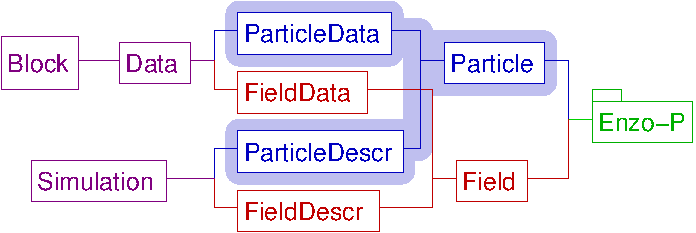
\includegraphics[width=2in]{data-classes-particle.pdf}
\end{center}

\begin{itemize}
\item \greencode{ParticleData}
\begin{itemize}
\item represents state-independent (intrinsic) data
\item associated with \greencode{Block}s (one object per mesh node)
\item stores arrays of particle data
\end{itemize}
\item \greencode{ParticleDescr}
\begin{itemize}
\item represents state-dependent (extrinsic) data
\item associated with \greencode{Simulation} objects (one per process)
\item describes how to interpret particle data (types, attributes, etc.)
\end{itemize}
\item \greencode{Particle}
\begin{itemize}
\item applications access particle data via \greencode{Particle} objects
\end{itemize}
\end{itemize}
\end{frame}

%----------------------------------------------------------------------

\begin{frame}[fragile,label=ss-particles] 
\secframetitle{How \code{Particle} objects store particle data}
\begin{minipage}{1.8in}
\includegraphics[width=2.0in]{particles-design.pdf} \ \\
\end{minipage} \ 
\begin{minipage}{2.5in}
\begin{itemize}
\item multiple particle \textit{types}
\item particles allocated in \textit{batches}
\begin{itemize}
\item fixed size arrays
\item fewer new/delete operations
\item efficient insert/delete operations
\item potentially useful for GPU's
\end{itemize}
\item batches store particle \textit{attributes}
\begin{itemize}
\item (position, velocity, mass, etc.)
\item 8,16,32,64-bit integers
\item 32,64,128-bit floats
\end{itemize}
\end{itemize}
\end{minipage}
\begin{itemize}
\item particle positions may be floating-point or integers
\begin{itemize}
\item floating-point for storing global positions
\item integers for \code{Block}-local coordinates
\begin{itemize}
\item solves reduced precision issue for deep hierarchies
\item less memory required for given accuracy
\end{itemize}
\end{itemize}
\end{itemize}


\end{frame}

%----------------------------------------------------------------------

\begin{frame}[fragile,label=ss-particles] 
\secframetitle{How particle data is communicated between Blocks}
\begin{itemize}
\item communication is required when particles move outside a Block 
\item this is done using a 4x4x4 array
\begin{itemize}
\item array contains pointers to ParticleData (PD) objects
\item one PD object per neighbor Block
\end{itemize}

\end{itemize}
\begin{minipage}{1.8in}
%\includegraphics<1>[width=2.0in]{particle-refresh-0.pdf}
%\includegraphics<2>[width=2.0in]{particle-refresh-1.pdf}
%\includegraphics<3>[width=2.0in]{particle-refresh-2.pdf}
%\includegraphics<4>[width=2.0in]{particle-refresh-3.pdf}
\includegraphics[width=2.0in]{particle-refresh-4.pdf}
\end{minipage} \ 
\begin{minipage}{2.7in}
\begin{itemize}
\item migrating particles are
\begin{itemize}
\item \code{scatter()}-ed to PD array objects
\item sent to associated neighbors
\item \code{gather()}-ed by neighbors
\end{itemize}
\item one sweep through particles
\item one communication step per neighbor
\item similar for refinement / coarsening
\end{itemize}
\end{minipage}
\end{frame}


 % How are particles used in the code?
%======================================================================
\NEWSEC
%======================================================================

\subsection{\ssMethods}

\begin{frame}[fragile,label=ss-methods] 
\secframetitle{\ssMethods}
\greenbf{Method classes implement numerical methods on \code{Block}s}
\ \\
\begin{tabbing}
xxxx\=xxxxxxxxxxxxxx\=\kill
\> \greencode{compute()} \> \redit{Apply the method to a} \greencode{block} \\
\> \greencode{name()}    \> \redit{Return the method name (e.g.} \redcode{"ppm"}) \\
\> \greencode{timestep()} \> \redit{Return maximum allowed timestep}
\end{tabbing}

\greentext{Current methods include}
\footnotesize
\begin{tabbing}
xxxx\=xxxxxxxxxxxxxxxxxxxxxxxxxxxxx\=\kill
\> \bluecode{EnzoMethodPpm} \> \redit{PPM hydrodynamics (Greg Bryan et al)} \\
\> \bluecode{EnzoMethodPpml} \> \redit{PPML ideal MHD (Sergey Ustyugov)} \\
\> \bluecode{EnzoMethodHeat} \> \redit{Forward Euler heat equation } \\
\> \bluecode{EnzoMethodGravityBiCGStab} \> \redit{BiCG-STAB gravity solver (Dan Reynolds)} \\
\> \bluecode{EnzoMethodGravityCg} \> \redit{CG gravity solver } \\
\> \bluecode{EnzoMethodGravityMg0} \> \redit{MG root-grid gravity solver  (incomplete)} \\
\> \bluecode{EnzoMethodGravityMlat} \> \redit{MG gravity solver  (incomplete)} \\
\> \bluecode{EnzoMethodGrackle} \> \redit{Grackle chemistry (Britton Smith) (incomplete)} \\
\> \bluecode{EnzoMethodTurbulence} \> \redit{Turbulent mixing (Alexei Kritsuk)}
\end{tabbing}
\end{frame}


 % What numerical methods are available?
%======================================================================
\NEWSEC
%======================================================================


\subsection{\ssInitialBoundary}

\begin{frame}[fragile,label=ss-initial-boundary] 
\secframetitle{\ssInitialBoundary}
\greenbf{Initial classes implement initial conditions}
\ \\
\begin{tabbing}
xxxx\=xxxxxxxxxxxxxxxxxxxx\=\kill
\> \greencode{enforce\_block()} \> \redit{Apply the initial conditions on a} \greencode{block}
\end{tabbing}

\greentext{Current initial conditions include}
\footnotesize
\begin{tabbing}
xxxx\=xxxxxxxxxxxxxxxxxxxxxxxxxxx\=\kill
\> \bluecode{InitialValue} \> \redit{Initialize from parameter file} \\
\> \bluecode{EnzoInitialImplosion2} \> \redit{Implosion test problem} \\
\> \bluecode{EnzoInitialSedovArray2} \> \redit{2D array of Sedov blasts  } \\
\> \bluecode{EnzoInitialSedovArray3} \> \redit{3D array of Sedov blasts} \\
\> \bluecode{EnzoInitialTurbulence} \> \redit{Turbulence initial conditions (Kritusk)  } \\
\> \bluecode{EnzoInitialGrackleTest} \> \redit{Grackle test problem (Britton) (incomplete)} \\
\> \bluecode{InitialFile} \> \redit{Initialize from a file (incomplete)  }
\end{tabbing}
\end{frame}

\begin{frame}[fragile,label=ss-boundary] 
\secframetitle{\ssInitialBoundary}
\greenbf{Boundary classes implement boundary conditions}
\ \\
\begin{tabbing}
xxxx\=xxxxxxxxxxxxxxxxxx\=\kill
\> \greencode{enforce()} \> \redit{Apply the boundary conditions on a} \greencode{block}
\end{tabbing}

\greentext{Current boundary conditions include}
\footnotesize
\begin{tabbing}
xxxx\=xxxxxxxxxxxxxxxxxxxxxxxxxxx\=\kill
\> \bluecode{EnzoBoundary} \> \redit{Reflecting and outflow (Greg Bryan)} \\
\> \bluecode{BoundaryPeriodic} \> \redit{Periodic} \\
\> \bluecode{BoundaryValue} \> \redit{Inflow}
\end{tabbing}
\end{frame}


 % What initial conditions are supported?
%======================================================================
\NEWSEC
%======================================================================


\subsection{\ssRefine}

\begin{frame}[fragile,label=ss-refine] 
\secframetitle{\ssRefine}
\greenbf{Refine classes implement refinement criteria}
\ \\
\begin{tabbing}
xxxx\=xxxxxxxxxx\=\kill
\> \greencode{apply()} \> \redit{Apply the refinement criteria on a} \greencode{block} \\
\> \greencode{name()} \> \redit{Return the name of the criteria (e.g.~"shock")} \greencode{block}
\end{tabbing}

\greentext{Current refine conditions include}
\footnotesize
\begin{tabbing}
xxxx\=xxxxxxxxxxxxxxxxxxxxx\=\kill
\> \bluecode{RefineSlope} \> \redit{refine on relative slope} \\
% ($\lvert\frac{x_{i+1}- x_{i-1}}{2h \cdot x_i}\rvert$)
\> \bluecode{RefineDensity} \> \redit{refine on density threshold} \\
\> \bluecode{RefineMask} \> \redit{refine according to level array} \\
\> \bluecode{RefineShear} \> \redit{refine on shear} \\
\> \bluecode{EnzoRefineShock} \> \redit{refine on shocks} \\
\> \bluecode{RefineMass} \> \redit{refine on minimum mass (not implemented)}
\end{tabbing}
\end{frame}


 % What refinement criteria are supported?
%======================================================================
\NEWSEC
%======================================================================

\subsection{\ssDesignSummary}

%----------------------------------------------------------------------

\begin{frame}[fragile,label=ss-design-summary] 
\secframetitle{\ssDesignSummary}

\begin{itemize}
\item Enzo-P / Cello has an \bluetext{object-oriented design}
\item Related classes grouped into \bluetext{components}
\item Classes are kept relatively simple
\item Field and (soon) Particle classes simplify implementing Methods
\item Enzo-P is implemented by inheriting from Cello classes
  \begin{tabbing}
xxxx\=xxxxxxxxxx\=\kill    
\> \greencode{Method} \> \redit{Numerical methods} \\
\> \greencode{Initial} \>  \redit{Initial conditions} \\
\> \greencode{Boundary} \>  \redit{Boundary conditions} \\
\> \greencode{Refine} \>  \redit{Refinement criteria} \\
\> \ \ \ \ \ \vdots  \> \ \ \ \ \ \vdots 
  \end{tabbing}
\end{itemize}
\vfill
\centerline{$\qed$}
\end{frame}

 % What refinement criteria are supported?
%%======================================================================
\NEWSEC
%======================================================================

\subsection{\ssStopping}

\begin{frame}[fragile,label=ss-stoppig] 
\secframetitle{\ssStopping}

class Stopping

\end{frame}

 % What stopping criteria are supported?
%%======================================================================
\NEWSEC
%======================================================================

\subsection{\ssClassesOrg}

\begin{frame}[fragile,label=ss-classes-org] 
\secframetitle{\ssClassesOrg}

\end{frame}

 % How are Enzo-P's classes organized?


  %======================================================================
\NEWMOD
%======================================================================

\section{\sControl}

%----------------------------------------------------------------------

\logo{\hfill\hyperlink{outline<1>}{\icon}}

\begin{frame}[fragile,label=s-control] 
\modframetitle{\sControl}
\small
\begin{center}
\begin{minipage}{3.25in}
\begin{enumerate}
\item \hyperlink{ss-control<1>}   {\BUTTON {\ssControl}}
\item \hyperlink{ss-adapt<1>}   {\BUTTON {\ssAdapt}}
\item \hyperlink{ss-refresh<1>}   {\BUTTON {\ssRefresh}}
\item \hyperlink{ss-control-summary<1>}   {\BUTTON {\ssControlSummary}}
\end{enumerate}
\end{minipage}
\end{center}
\end{frame}

\logo{\hfill\hyperlink{s-control<1>}{\icon}}

%======================================================================
\NEWSEC
%======================================================================

\subsection{\ssControl}

\begin{frame}[fragile,label=ss-control] 
\secframetitle{\ssControl}

\bluebf{Simulation evolution is controlled in} \bluecode{control\_charm.cpp}

\tikzstyle{decision} = [diamond, draw, fill=blue!20, 
    text width=4.5em, text badly centered, node distance=3cm, inner sep=0pt]
\tikzstyle{block} = [rectangle, draw, fill=blue!20, 
    text width=5em, text centered, rounded corners, minimum height=4em]
\tikzstyle{line} = [draw, -latex']
\tikzstyle{cloud} = [draw, ellipse,fill=red!20, node distance=3cm,
    minimum height=2em]
\ \\
\begin{tikzpicture}[node distance = 3cm, auto]
   \node [block] (init) {Initialize};
   \node [block,below of=init, node distance = 2cm] (adapt) {Adapt};
   \node [block,right of=adapt] (output) {Output};
   \node [block,right of=output] (stopping) {Stopping criteria};
   \node [block,right of=stopping] (compute) {Compute}; 
   \node [block, above of=compute, node distance = 2cm] (refresh) {Refresh};
   \node [coordinate, below of=compute, node distance = 1.5cm] (computenode) {};
   \node [coordinate, below of=adapt, node distance = 1.5cm] (adaptnode) {};

   \path [line] (init) -- (adapt);   
   \path [line] (adapt) -- (output);   
   \path [line] (output) -- (stopping);   
   \path [line] (stopping) -- (compute);   
   \path [line] (compute) -- (refresh);   
   \path [line] (refresh) -- (compute);   
%   \path [line] (compute) -- (adapt);   
 \path [line] (compute.south) -|  (computenode) -- (adaptnode) |- (adapt.south);
\end{tikzpicture}

\end{frame}

 % How are phases of the computation controlled?
%======================================================================
\NEWSEC
%======================================================================

\subsection{\ssAdapt}

%----------------------------------------------------------------------

\begin{frame}[fragile,label=ss-adapt] 
\secframetitle{\ssAdapt}
\bluebf{Mesh refinement proceeds in several steps}

\begin{enumerate}
\item Apply refinement criteria (\code{Refine})
\item Tell neighbor \code{Block}s your desired level
\begin{itemize}
\item \code{Block}s form a chare array
\item remote entry method call to neighbor blocks
\end{itemize}
\item Receive neighbor level
\begin{itemize}
\item entry method
\item called by neighbors
\end{itemize}
\item Update own level if needed (goto \bluebf{2})
\item Exit after \blueit{quiescence}
\begin{itemize}
\item no processor is executing an entry point
\item no messages are awaiting processing
\item and no messages in-flight
\end{itemize}
\end{enumerate}
\end{frame}

%----------------------------------------------------------------------

\begin{frame}[fragile]
\secframetitle{\ssAdapt}
\begin{center}
\begin{minipage}{3in}
\includegraphics[width=3in]{amr-2.pdf}
\end{minipage}
\end{center}
\pause
\begin{itemize}
\item \greentext{temporal level jump criterion}
\pause
\item \magentatext{spacial level jump criterion}
\end{itemize}
\end{frame}

%----------------------------------------------------------------------

\begin{frame}[fragile] 
\secframetitle{\ssAdapt}
\blockblue
\begin{center}
\begin{minipage}{2.5in}
\ANIMATEGRAPHICS{width=2.5in}{40}{Images/Circle/mesh-00}{475}{951}
\end{minipage}
\end{center}
\end{frame}
 % How does Cello implement AMR?
%======================================================================
\NEWSEC
%======================================================================

\subsection{\ssRefresh}

%----------------------------------------------------------------------

\begin{frame}[fragile,label=ss-refresh] 
\secframetitle{\ssRefresh}
\framesubtitle{Neighbor in same refinement level}
%\blockblue
\begin{minipage}{2.0in}
\begin{center}
   \includegraphics[width=2.0in]{refresh-same.pdf} \ \\
\end{center}
\end{minipage} \ 
\begin{minipage}{2.1in}
\begin{enumerate}
\item Face data copied to array
\begin{itemize}
\item \bluecode{FieldFace} object
\end{itemize}
\item Array sent to neighbor
\begin{itemize}
\item chare entry method
\item array sent as message
\end{itemize}
\item Array copied to ghost zones
\end{enumerate}
\end{minipage}
\vspace{0.2in}
\ \\
\ \\
\bluetext{Refresh ends when arrays from all neighbors have been received.}
\end{frame}

%----------------------------------------------------------------------

\begin{frame}[fragile]
\secframetitle{\ssRefresh}
\framesubtitle{Neighbor in coarser refinement level}
%\blockblue
\begin{minipage}{2.0in}
\begin{center}
   \includegraphics[width=2.0in]{refresh-coarse.pdf} \ \\
\end{center}
\end{minipage} \ 
\begin{minipage}{2.1in}
\begin{enumerate}
\item Face data coarsened to array
\begin{itemize}
\item \code{Restrict} object
\item \code{FieldFace} array
\end{itemize}
\item Array sent to neighbor
\item Array copied to ghost zones
\end{enumerate}
\end{minipage}
\end{frame}

%----------------------------------------------------------------------

\begin{frame}[fragile]
\secframetitle{\ssRefresh}
\framesubtitle{Neighbor in finer refinement level}
%\blockblue
\begin{minipage}{2.0in}
\begin{center}
   \includegraphics[width=2.0in]{refresh-fine.pdf} \ \\
\end{center}
\end{minipage}
\begin{minipage}{2.1in}
\begin{enumerate}
\item Face data copied to array
\item Array sent to neighbor
\item Data interpolated to ghost zones
\begin{itemize}
\item \code{Prolong} object
\end{itemize}
\end{enumerate}
\end{minipage}
\end{frame}

%----------------------------------------------------------------------

%\secframetitle{\ssRefresh}
%%\blockblue
%\begin{center}
%\begin{tabular}{|c|c|c|} \hline
%\begin{minipage}{1.0in}
%\onslide<1-> \vspace{0.1in} $\boldsymbol{L}$ \textcolor{red}{$\Rightarrow L$} \vspace{0.1in} \hfill  \ \\
%   \includegraphics<1->[height=0.8in]{n-send-same.pdf} \ \\
%\end{minipage} \pause &
%\begin{minipage}{1.0in}
%\onslide<2-> \vspace{0.1in} $\boldsymbol{L}$ \textcolor{red}{$\Rightarrow L-1$} \vspace{0.1in} \hfill  \ \\ 
%   \includegraphics<2->[height=0.8in]{n-send-coarse.pdf} \ \\
%\end{minipage} \pause  &
%\begin{minipage}{1.0in}
%\onslide<3->  \vspace{0.1in} $\boldsymbol{L}$ \textcolor{red}{$\Rightarrow L+1$}\vspace{0.1in} \hfill \ \\ 
%   \includegraphics<3->[height=0.8in]{n-send-fine.pdf} \ \\
%\end{minipage} \pause \\ \hline
%\begin{minipage}{1.0in}
%\onslide<4->  \vspace{0.1in} \hfill \textcolor{blue}{$L \Rightarrow$} $ \boldsymbol{L}$ \vspace{0.1in}  \ \\
%   \includegraphics<4->[height=0.8in]{n-recv-same.pdf} \ \\
%\end{minipage}  &
%\begin{minipage}{1.0in}
%\onslide<5->  \vspace{0.1in} \hfill \textcolor{blue}{$L+1 \Rightarrow$} $ \boldsymbol{L}$\vspace{0.1in}  \ \\
%   \includegraphics<5->[height=0.8in]{n-recv-fine.pdf} \ \\
%\end{minipage}  &
%\begin{minipage}{1.0in}
%\onslide<6->   \vspace{0.1in} \hfill \textcolor{blue}{$L-1 \Rightarrow$} $ \boldsymbol{L}$\vspace{0.1in}  \ \\  
%   \includegraphics<6->[height=0.8in]{n-recv-coarse.pdf} \ \\
%\end{minipage} \\ \hline
%\end{tabular}
%\end{center}
%\end{frame}

 % How does Cello exchange data between blocks?
%======================================================================
\NEWSEC
%======================================================================

\subsection{\ssControlSummary}

%----------------------------------------------------------------------

\begin{frame}[fragile,label=ss-control-summary] 
\secframetitle{\ssControlSummary}

\vfill
\centerline{$\qed$}
\end{frame}

 % How does Cello exchange data between blocks?

  %======================================================================
\NEWMOD
%======================================================================

\section{\sDevel}

%----------------------------------------------------------------------

\logo{\hfill\hyperlink{outline<1>}{\icon}}

\begin{frame}[fragile,label=s-devel] 
\modframetitle{\sDevel}
\small
\begin{center}
\begin{minipage}{3.25in}
\begin{enumerate}
\item \hyperlink{ss-devel-coding<1>}   {\BUTTON {\ssDevelCoding}}
\item \hyperlink{ss-add-parameter<1>}   {\BUTTON {\ssAddParameter}}
\item \hyperlink{ss-add-method<1>}   {\BUTTON {\ssAddMethod}}
\item \hyperlink{ss-add-initial<1>}   {\BUTTON {\ssAddInitial}}
\item \hyperlink{ss-add-boundary<1>}   {\BUTTON {\ssAddBoundary}}
\item \hyperlink{ss-add-refine<1>}   {\BUTTON {\ssAddRefine}}
\item \hyperlink{ss-add-test<1>}   {\BUTTON {\ssAddTest}}
\item \hyperlink{ss-devel-summary<1>} {\BUTTON {\ssDevelSummary}}
\end{enumerate}
\end{minipage}
\end{center}
\end{frame}

\logo{\hfill\hyperlink{s-devel<1>}{\icon}}

%======================================================================
\NEWSEC
%======================================================================

\subsection{\ssDevelCoding}

\begin{frame}[fragile,label=ss-devel-coding] 
\secframetitle{\ssDevelCoding}
\framesubtitle{Naming things}
%\footnotesize

\begin{itemize}

\item {\bluebf{Naming classes}}
%
\begin{tabbing}
xxxxxxxxxxxxxxxxxxxxxx\=xxxxxxxxxx\=\kill
\> \greenit{methods} \' \ \redcode{Enzo}\redcode{Method}\redit{Name} \\
\> \greenit{initial conditions} \'  \ \redcode{Enzo}\redcode{Initial}\redit{Name} \\
\> \greenit{boundary conditions} \'  \ \redcode{Enzo}\redcode{Boundary}\redit{Name}
\end{tabbing}
%
\item {\normalsize\bluebf{Naming files}}
%
\begin{tabbing}
xxxxxxxxxxxxxxxxxxxxxx\=xxxxxxxxxx\=\kill
\> \greenit{methods} \' \ \redcode{enzo\_Enzo}\redcode{Method}\redit{Name}\redcode{.[hc]pp} \\
\> \greenit{initial conditions} \'  \ \redcode{enzo\_Enzo}\redcode{Initial}\redit{Name}\redcode{.[hc]pp} \\
\> \greenit{boundary conditions} \'  \ \redcode{enzo\_Enzo}\redcode{Boundary}\redit{Name}\redcode{.[hc]pp}
\end{tabbing}
\end{itemize}

\end{frame}

%----------------------------------------------------------------------    

\begin{frame}[fragile] 
\secframetitle{\ssDevelCoding}
\framesubtitle{Naming things}
%
\begin{itemize}
%
\item {\normalsize\bluebf{Naming class methods}}
\begin{tabbing}
xxxxxxxxxxxxxxxxxxxxxx\=xxxxxxxxxxxxxxxxxx\=\kill
\> \greenit{public methods} \' \ \bluecode{thing\_1}\code{()} \\
\> \greenit{private methods} \' \ \bluecode{thing\_2}\redcode{\_}\code{()} \\
\> \greenit{entry methods} \' \ \redcode{p\_}\bluecode{blah}\code{()} \\
\> \greenit{reduction entry methods} \' \ \redcode{r\_}\bluecode{reduce}\code{()}
\end{tabbing}
%
\item {\normalsize\bluebf{Naming variables}}
\begin{tabbing}
xxxxxxxxxxxxxxxxxxxxxx\=xxxxxxxxxxxxxxxxxx\=\kill
\> \greenit{Array dimensions} \'  \   \bluecode{mx},\bluecode{my},\bluecode{mz} \\
\> \greenit{Active region size} \' \ \bluecode{nx},\bluecode{ny},\bluecode{nz} \\
\> \greenit{Ghost zone depth} \' \ \bluecode{gx},\bluecode{gy},\bluecode{gz} \\
\> \greenit{Loop variables} \'   \ \bluecode{ix},\bluecode{iy},\bluecode{iz} 
\end{tabbing}

\end{itemize}

\end{frame}

%----------------------------------------------------------------------    

\begin{frame}[fragile,label=field-access] 
\secframetitle{\ssDevelCoding}
\framesubtitle{Accessing field data}
\bluebf{Accessing field data is relatively easy}
\scriptsize
\newcommand{\gc}[1]{\greencode{#1}}
\newcommand{\bc}[1]{\bluecode{#1}}
\newcommand{\rc}[1]{\redcode{#1}}
\newcommand{\oc}[1]{\orangecode{#1}}
\newcommand{\mc}[1]{\magentacode{#1}}

\begin{semiverbatim}
     \gc{Field} \oc{field} = block->data()->field();

     id = field.field_id(\redcode{"density"});

     field.dimensions(id, &mx, &my, &mz);
     field.size          (&nx, &ny, &nz);
     field.ghost_depth(id &gx, &gy, &gz);

     \gc{double} * \oc{d} = (\gc{double} *) field.values(id);

     \mc{for} (\gc{int} \oc{iz}=gz; iz<gz+nz; iz++) \{
        \mc{for} (\gc{int} \oc{iy}=gy; iy<gy+ny; iy++) \{
           \mc{for} (\gc{int} \oc{ix}=gx; ix<gx+nx; ix++) \{
              \gc{int} \oc{i} = ix + mx*(iy + my*iz);
              d[i] = tiny ;
           \}
        \}
     \}
\end{semiverbatim}
\end{frame}
 % What are some coding guidelines for Enzo-P developers?
%======================================================================
\NEWSEC
%======================================================================

\subsection{\ssAddParameter}

\begin{frame}[fragile,label=ss-add-parameter] 
\secframetitle{\ssAddParameter}

\begin{enumerate}
\item \bluetext{Add parameter declaration to }[\redcode{Enzo}]\redcode{Config}
\begin{tabbing}
xxxxxxxxxxxxxxxxxx\=xxxxxxxxxxxxxx\=\kill
\greentext{Cello parameter}: \> \greencode{src/Cello/parameters\_Config.hpp} \\
\greentext{Enzo parameter}: \> \greencode{src/Enzo/enzo\_EnzoConfig.hpp}
\end{tabbing}
\item \bluetext{Read parameter value in }[\redcode{Enzo}]\redcode{Config}
\begin{tabbing}
xxxxxxxxxxxxxxxxxx\=xxxxxxxxxxxxxx\=\kill
\greentext{Cello parameter}: \> \greencode{src/Cello/parameters\_Config.cpp} \\
\greentext{Enzo parameter}: \> \greencode{src/Enzo/enzo\_EnzoConfig.cpp}
\end{tabbing}
\item \bluetext{Add \charm\ pack/unpack call to} [\redcode{Enzo}]\redcode{Config}\code{::}\redcode{pup()}
\item \bluetext{Update documentation}
\begin{tabbing}
xxxxxxxxxxxxxxxxxx\=xxxxxxxxxxxxxx\=\kill
\greencode{cello-doc/source/parameters-list.rst}
\end{tabbing}
\item \bluetext{Access parameter via} [\bluecode{Enzo}]\bluecode{Config}
\end{enumerate}

\end{frame}

%----------------------------------------------------------------------

\begin{frame}[fragile]
\secframetitle{\ssAddParameter}
\footnotesize
\bluebf{\normalsize 1.~Add parameter declaration to} \greentext{enzo\_EnzoConfig.hpp}
\begin{itemize}
\item \bluetext{Name parameter according to owning class, e.g.~for} \redcode{MethodGravityMg}
\begin{semiverbatim}
  \code{int}     \redtext{method_gravity_mg_iter_max;}
\end{semiverbatim}
\end{itemize}
\ \\
\bluebf{\normalsize 2.~Read parameter value in} \greencode{enzo\_EnzoConfig.cpp}
\begin{semiverbatim}
  \redtext{method_gravity_mg_iter_max} = \redtext{p}->\bluetext{value_integer}
    (\orangetext{"Method:gravity_mg:iter_max"},\orangetext{10});
\end{semiverbatim}
\ \\
\bluebf{\normalsize 3.~Add \charm\ pack/unpack call to} \greencode{enzo\_EnzoConfig.cpp}
\begin{semiverbatim}
void \bluetext{EnzoConfig}::\bluetext{pup} (\greentext{PUP::er} &\redtext{p}) \{
          \vdots
  \redtext{p} | \redtext{method_gravity_cg_iter_max};
          \vdots
\}
\end{semiverbatim}


\end{frame}

%----------------------------------------------------------------------

\begin{frame}[fragile]
\secframetitle{\ssAddParameter}

\bluebf{4.~Update documentation in enzo/-doc/source/parameters-list.rst} \\
\scriptsize
\begin{semiverbatim}
\greencode{:Parameter:}  \magentacode{:p:}\greencode{`Method`} : \magentacode{:p:}\greencode{`gravity_mg`} : \magentacode{:p:}\greencode{`iter_max`}

\greencode{:Summary:} \magentacode{:s:} \greencode{`Maximum number of multigrid cycles.`}
\greencode{:Type:}    \magentacode{:t:}\greencode{`int`}
\greencode{:Default:} \magentacode{:d:}\greencode{`10`}
\greencode{:Scope:}     Enzo

\magentacode{:e:}\greencode{`Maximum number of cycles of the multigrid solver.`}
\end{semiverbatim}
\ \\
\begin{center}
\includegraphics[width=3.5in]{mg_iter_max.png}
\end{center}
\end{frame}

%----------------------------------------------------------------------

\begin{frame}[fragile]
\secframetitle{\ssAddParameter}
% 
 \bluebf{5.~Access parameter via \greencode{EnzoConfig} class \redcode{enzo\_config}}
\footnotesize
 \begin{semiverbatim}
\bluecode{Method} * \bluecode{EnzoProblem}::\greencode{create_method_} ()
 \{
    if (\redcode{name} == \orangecode{"ppm"}) \{
            \vdots
    \} else if (\redcode{name} == \orangecode{"gravity_mg"}) \{
       \redcode{method} = new \bluecode{EnzoMethodGravityMg0}
 	             (\redcode{field_descr}, \redcode{rank},
                    \vdots
                \redcode{enzo_config}->\redcode{method_gravity_mg_iter_max},
                    \vdots
               );
     \} \ldots
\}

\end{semiverbatim}
\end{frame}
% 
 % How do I add a new input parameter to Enzo-P?
%======================================================================
\NEWSEC
%======================================================================

\subsection{\ssAddMethod}

\begin{frame}[fragile,label=ss-add-method] 
\secframetitle{\ssAddMethod}
\textbf{Suppose we wish to add a FE heat equation solver to \enzop.} \\ \ \\
\centerline{\Large \greentext{$u_t - \alpha \nabla^2 u = 0$}}
\begin{center}
\rowcolors[]{1}{blue!5}{blue!10}
  \begin{tabular}{l}
  \uncover<2->{\addclass{1.~\textbf{Create \code{EnzoMethodHeat} class}}} \\
  \uncover<3->{\addclass{2.~Include \code{enzo\_EnzoMethodHeat.hpp} file}} \\
  \uncover<4->{\addconstruct{3.~Call \code{EnzoMethodHeat} constructor}} \\
  \uncover<5->{\addparam{4.~Declare \code{EnzoMethodHeat} parameters}} \\
  \uncover<6->{\addparam{5.~Read in \code{EnzoMethodHeat} parameters}}  \\
  \uncover<7->{\addcharm{6.~Update \charm\ control file \code{enzo.ci}}} \\
  \uncover<8->{\addtest{7.~Create \code{test\_heat.in} test problem}} \\
%  \uncover<8->{\orow{Add \code{test\_heat} to the other regression tests}} \\
%  \uncover<9->{\erow{Display the \code{test\_heat} test results in \code{index.php}}} \\
  \uncover<9->{\addtest{8.~Run the test and verify test results}}
  \end{tabular}
\end{center}
\end{frame}

%----------------------------------------------------------------------

\begin{frame}[fragile] 
\secframetitle{\ssAddMethod}
\framesubtitle{1.~Create an \code{EnzoMethodHeat} class}

\addclassbf{Create header and source code files}
      \begin{itemize}
      
         \item \textcolor{red!50!black}
             {\code{src/Enzo/enzo\_EnzoMethodHeat.hpp}}
         \item \textcolor{red!50!black}
             {\code{src/Enzo/enzo\_EnzoMethodHeat.cpp}}
      \end{itemize}
      \pause
      \bluebf{Implement virtual functions}
      \begin{itemize}
      
          \item \textcolor{blue!50!black}
              {\code{EnzoMethodHeat::EnzoMethodHeat} ()}
          \item \textcolor{blue!50!black}
              {\code{EnzoMethodHeat::compute} ()}
          \item \textcolor{blue!50!black}
              {\code{EnzoMethodHeat::timestep} ()}
          \item \textcolor{blue!50!black}
              {\code{EnzoMethodHeat::pup} ()}
      \end{itemize}
\end{frame}

\definecolor{kcol}{rgb}{0.5,0.0,0.5}
\definecolor{ccol}{rgb}{0.0,0.5,0.0}
\definecolor{mcol}{rgb}{0.8,0.0,0.0}
\definecolor{fcol}{rgb}{0.0,0.0,0.8}
\definecolor{tcol}{rgb}{0.0,0.8,0.0}
\definecolor{vcol}{rgb}{0.8,0.3,0.0}

%----------------------------------------------------------------------

\begin{frame}[fragile] 
\secframetitle{\ssAddMethod}
\framesubtitle{1.~Create an \code{EnzoMethodHeat} class}
\addclassbf{Create the \code{src/Enzo/EnzoMethodHeat.hpp} header file}
\footnotesize
\begin{tabbing}
xxxxxxx\=xxxxxx\=\kill
\textbf<2>{\code{
\color<1,2>{kcol} class
\color<1,2>{ccol} EnzoMethodHeat
\color<1,2>{black}:\ \color<1,2>{kcol}public
\color<1,2>{ccol} Method
\color<1,2>{black}     \{ 
}}  \\
 \\[-2ex]
\code{
\color<1>{kcol} public:
\color<1>{mcol} // interface
} \\
\> \textbf<3>{\code{
\color<1,3>{fcol}  EnzoMethodHeat 
\color<1,3>{black} ( 
\color<1,3>{tcol} double 
\color<1,3>{vcol} alpha 
\color<1,3>{black} ,  
\color<1,3>{tcol} double 
\color<1,3>{vcol}  courant 
\color<1,3>{black} );
 }} \\
\> \textbf<4>{\code{
\color<1,4>{kcol} virtual 
\color<1,4>{kcol} void  
\color<1,4>{fcol} compute 
\color<1,4>{black} ( 
\color<1,4>{tcol} Block  
\color<1,4>{black} * 
\color<1,4>{vcol} block
\color<1,4>{black}) 
\color<1,4>{kcol}  throw 
\color<1,4>{black}();
}} \\
\> \textbf<4>{\code{
\color<1,4>{kcol}  virtual 
\color<1,4>{kcol}  double 
\color<1,4>{fcol}  timestep 
\color<1,4>{black}    ( 
\color<1,4>{tcol}  Block  
\color<1,4>{black}  * 
\color<1,4>{vcol}  block 
\color<1,4>{black}   )  
\color<1,4>{kcol}    throw 
\color<1,4>{black}    ();
}} \\
\> \textbf<5>{\code{
\color<1,5>{fcol}EnzoMethodHeat
\color<1,5>{black} () \{\};
}} \\
\> \textbf<5>{\code{
\color<1,5>{fcol} EnzoMethodHeat
\color<1,5>{black} (
\color<1,5>{tcol} CkMigrateMessage
\color<1,5>{black}  *
\color<1,5>{vcol} m
\color<1,5>{black} ) \{\}
}} \\
\> \textbf<5>{\code{
\color<1,5>{fcol}PUPable\_decl\color<1,5>{black}(\color<1,5>{tcol}EnzoMethodHeat\color<1,5>{black} );
}} \\
\> \textbf<5>{\code{
\color<1,5>{kcol} void
\color<1,5>{fcol} pup
\color<1,5>{black} (
\color<1,5>{tcol}PUP::er 
\color<1,5>{black}\&
\color<1,5>{vcol}p
\color<1,5>{black} )
}}
 \\
\> \textbf<5>{\code{
\color<1,5>{black} \{ 
\color<1,5>{tcol}Method\color<1,5>{black}::pup(
\color<1,5>{vcol}p
\color<1,5>{black} ); 
\color<1,5>{vcol}p
\color<1,5>{black} |
\color<1,5>{vcol} alpha\_
\color<1,5>{black} ;
\color<1,5>{vcol} p
\color<1,5>{black} |
\color<1,5>{vcol}courant\_
\color<1,5>{black} ;  \};
}} \\
\\[-2ex]
\textbf<6>{\code{
\color<1,6>{kcol} protected
\color<1,6>{black}:
\color<1,6>{mcol} // methods
}} \\
\> \textbf<6>{\code{
\color<1,6>{kcol} template 
\color<1,6>{black} $<$
\color<1,6>{kcol} class
\color<1,6>{tcol}  T
\color<1,6>{black} $>$ 
\color<1,6>{kcol} void
\color<1,6>{fcol}  compute\_ 
\color<1,6>{black} (
\color<1,6>{tcol} Block
\color<1,6>{black} * 
\color<1,6>{vcol} block
\color<1,6>{black} ,
\color<1,6>{tcol} T
\color<1,6>{black} * 
\color<1,6>{vcol} Unew
\color<1,6>{black} );
%\color<1,6>{kcol} const throw
%\color<1,6>{black} ();
}} \\
\\[-2ex]
\textbf<3>{\code{
\color<1,3>{kcol} protected
\color<1,3>{black} :
\color<1,3>{mcol}  // attributes
}} \\
\> \textbf<3>{\code{
\color<1,3>{tcol} double
\color<1,3>{vcol}  alpha\_
\color<1,3>{black} ;
}} \\
\> \textbf<3>{\code{
\color<1,3>{tcol} double
\color<1,3>{vcol}  courant\_
\color<1,3>{black} ;
}} \\
\textbf<2>{\code{
\color<1,2>{black} \};
}} \\
\end{tabbing}
\end{frame}

%-----------------------------------------------------------------------

\begin{frame}[fragile] 
\secframetitle{\ssAddMethod}
\framesubtitle{1.~Create an \code{EnzoMethodHeat} class}
\addclassbf{Implement the \code{EnzoMethodHeat::compute()} method}
\scriptsize
\begin{semiverbatim}
\keyword{void} \type{EnzoMethodHeat}::\function{compute} ( \type{Block} * \variable{block}) throw()
\{
  \keyword{if} (\variable{block}->\function{is_leaf}()) \{

     \type{Field} \variable{field} = \variable{block}->\function{data}()->\function{field}();

     \keyword{const} \type{int} \variable{id_temp} = \variable{field}.\function{field_id} (\valuetext{"temperature"});

     \type{void} *    \variable{t} = \variable{field}.\function{values} (\variable{id_temp});
     \keyword{const} \type{int} \variable{p} = \variable{field}.\function{precision} (\variable{id_temp});

     \keyword{if}      (\variable{p} == \valuetext{precision_single})    \function{compute_} (\variable{block},(\keyword{float} *)\variable{t});
     \keyword{else if} (\variable{p} == \valuetext{precision_double})    \function{compute_} (\variable{block},(\keyword{double}*)\variable{t});
     \keyword{else if} (\variable{p} == \valuetext{precision_quadruple}) \function{compute_} (\variable{block},(\keyword{long double}*) \variable{t});
     \keyword{else} 
       \function{ERROR1}(\valuetext{"EnzoMethodHeat()"}, \valuetext{"precision %d not recognized"}, \variable{p});
  \}
  \variable{block}->\function{compute_done}();
\}
\end{semiverbatim}
\end{frame}

%----------------------------------------------------------------------

\begin{frame}[fragile] 
\secframetitle{\ssAddMethod}
\framesubtitle{1.~Create an \code{EnzoMethodHeat} class}
\addclassbf{Implement the \code{EnzoMethodHeat::compute\_()} method}
\scriptsize
\begin{semiverbatim}
\keyword{template} <\keyword{class} \type{T}>
\type{void} \type{EnzoMethodHeat}::\function{compute_} (\type{T} * \variable{Unew}) \keyword{const throw}()
\{
   \type{Field} \variable{field}  = \variable{block}->\function{data}()->\function{field}();

   \keyword{const} \type{int} \variable{id_temp} = \type{field}.\function{field_id} (\valuetext{"temperature"});

   \type{field}.\function{dimensions}  (\variable{id_temp},&\variable{mx},&\variable{my},&\variable{mz});
   \type{field}.\function{size}                (&\variable{nx},&\variable{ny},&\variable{nz});
   \type{field}.\function{ghost_depth} (\variable{id_temp},&\variable{gx},&\variable{gy},&\variable{gz});
        \vdots
\end{semiverbatim}
\end{frame}

%----------------------------------------------------------------------

\begin{frame}[fragile] 
\secframetitle{\ssAddMethod}
\framesubtitle{1.~Create an \code{EnzoMethodHeat} class}
\addclassbf{Implement the \code{EnzoMethodHeat::compute\_()} method}
\begin{semiverbatim}\scriptsize
        \vdots
   \keyword{for} (\type{int} \variable{iz}=\variable{gz}; \variable{iz}<\variable{gz}+\variable{nz}; \variable{iz}++) \{
      \keyword{for} (\type{int} \variable{\variable{iy}}=\variable{gy}; \variable{iy}<\variable{gy}+\variable{ny}; \variable{iy}++) \{
         \keyword{for} (\type{int} \variable{ix}=\variable{gx}; \variable{ix}<\variable{gx}+\variable{\variable{nx}}; \variable{ix}++) \{

            \type{int} \variable{i} = \variable{ix} + \variable{mx}*(\variable{\variable{iy}} + \variable{my}*\variable{iz});

            \type{double} \variable{Uxx} = \variable{dxi}*(\variable{U}[\variable{i}-\variable{idx}] - \valuetext{2}*\variable{U}[\variable{i}] + \variable{U}[\variable{i}+\variable{idx}]);
            \type{double} \variable{Uyy} = \variable{dyi}*(\variable{U}[\variable{i}-\variable{idy}] - \valuetext{2}*\variable{U}[\variable{i}] + \variable{U}[\variable{i}+\variable{idy}]);
            \type{double} \variable{Uzz} = \variable{dzi}*(\variable{U}[\variable{i}-\variable{idz}] - \valuetext{2}*\variable{U}[\variable{i}] + \variable{U}[\variable{i}+\variable{idz}]);

            \variable{Unew}[\variable{i}] = \variable{U}[\variable{i}] + \variable{alpha}_*\variable{dt}*(\variable{Uxx} + \variable{Uyy} + \variable{Uzz});
         \}
      \}
   \}
\}
\end{semiverbatim}
\end{frame}

%----------------------------------------------------------------------

\begin{frame}[fragile] 
\secframetitle{\ssAddMethod}
\framesubtitle{2.~Include the \code{enzo\_EnzoMethodHeat.hpp} file}
\addclassbf{Update \code{src/Enzo/\_enzo.hpp}}
%
\begin{semiverbatim}
       \vdots
   #include "enzo_EnzoMethodPpm.hpp"
   #include "enzo_EnzoMethodPpml.hpp"
   #\keyword{include} \valuetext{"enzo_EnzoMethodHeat.hpp"}

   #include "enzo_EnzoProlong.hpp"
       \vdots
\end{semiverbatim}


\end{frame}

%----------------------------------------------------------------------

\begin{frame}[fragile] 
\secframetitle{\ssAddMethod}
\framesubtitle{3.~Call the \code{EnzoMethodHeat} constructor}

\addconstructbf{Update \code{src/Enzo/enzo\_EnzoProblem.cpp}}
\footnotesize
\begin{semiverbatim}
   Method * EnzoProblem::create_method_ (\dots)
   \{
         \vdots
      if (type == "ppm") \{
          method = new EnzoMethodPpm;
      \} else if (type == "ppml") \{
          method = new EnzoMethodPpml;
      \} \keyword{else if} (\variable{type} == \valuetext{"heat"}) \{
          \variable{method} = \keyword{new} \type{EnzoMethodHeat}
             (\variable{enzo_config->method_heat_alpha,}
              \variable{enzo_config->field_courant});
      \} else if
         \vdots
   \}
\end{semiverbatim}

\end{frame}

%----------------------------------------------------------------------

\begin{frame}[fragile, label=sss-add-parameters] 
\secframetitle{\ssAddMethod}
\framesubtitle{4.~Declare any \code{EnzoMethodHeat} parameters}

\addparambf{Update \code{src/Enzo/enzo\_EnzoConfig.hpp}}
\footnotesize
\begin{semiverbatim}
   class EnzoConfig : public Config \{
        \vdots 
   public: // attributes
        \vdots
     std::string      interpolation_method;

     \comment{// EnzoMethodHeat}
     \keyword{double}           \variable{method_heat_alpha};
        \vdots 
   \};
\end{semiverbatim}

\end{frame}

%======================================================================

\begin{frame}[fragile] 
\secframetitle{\ssAddMethod}
\framesubtitle{5.~Read in the \code{EnzoMethodHeat} parameters}

\addparambf{Update \code{src/Enzo/enzo\_EnzoConfig.cpp}}
\footnotesize
\begin{semiverbatim}
   void EnzoConfig::read(\dots)
   \{
        \vdots
      interpolation_method = p->value_string 
        ("Field:interpolation_method","SecondOrderA");

      \variable{method_heat_alpha} = \variable{p}->\function{value_float}
        (\valuetext{"Method:heat:alpha"},\valuetext{1.0});

      method_null_dt = p->value_float 
        ("Method:null:dt",std::numeric_limits<double>::max());
        \vdots
   \}
\end{semiverbatim}

\end{frame}

%======================================================================

\begin{frame}[fragile] 
\secframetitle{\ssAddMethod}
\framesubtitle{6.~Update the \charm\ control file \code{enzo.ci}}

\addcharmbf{Update \code{src/Enzo/enzo.ci}}
\footnotesize
\begin{semiverbatim}
   module enzo \{
       \vdots
     PUPable EnzoInitialImplosion2;
     PUPable EnzoInitialSedovArray2;
     PUPable EnzoInitialSedovArray3;
     PUPable EnzoMethodPpm;
     PUPable EnzoMethodPpml;
     \type{PUPable} \variable{EnzoMethodHeat};
     PUPable EnzoProblem;
       \vdots
   \};
\end{semiverbatim}
\end{frame}


%======================================================================

\begin{frame}[fragile] 
\secframetitle{\ssAddMethod}
\framesubtitle{7.~Create a \code{test\_heat.in} test problem}
\addtestbf{Create \code{input/test\_heat.in}}
\scriptsize
\vspace{-0.15in}
\begin{semiverbatim}
      \vdots
   \group{Method} \{
     \parameter{list} = [\valuetext{"heat"}]; 
     \subgroup{heat} \{ \parameter{alpha} = \valuetext{1.0}; \} 
   \}
\pause
   \group{Field} \{
      \parameter{list} = [\valuetext{"temperature"}];
      \parameter{courant} = \valuetext{0.5};
   \}
\pause
   \group{Adapt} \{
      \parameter{list} = [\valuetext{"slope"}];
      \subgroup{slope} \{
         \parameter{type} = \valuetext{"slope"};
         \parameter{field_list} = [\valuetext{"temperature"}];
      \}
   \}
\end{semiverbatim}

\end{frame}

%----------------------------------------------------------------------

% \begin{frame}[fragile] 
% \secframetitle{\ssAddMethod}
% \framesubtitle{Add \code{test\_heat} to the other regression tests}
% 
% \code{test/SConscript}
% 
% \begin{center}
% \begin{minipage}{3.0in}
% \blockblue
% \begin{block}<+->{\textbf{\code{src/Enzo/enzo\_EnzoProblem.cpp}}}
% \footnotesize
% \begin{semiverbatim}
% 
% test/SConscript:# MethodHeat tests
% test/SConscript:Clean(env\_mv\_out.RunSerial ('test\_method\_heat-1.unit',bin% \_path + '/enzo-p', 
% test/SConscript:		ARGS='input/method\_heat-1.in'),
% test/SConscript:      [Glob('#/' + test\_path + '/method\_heat-1*.png'),
% test/SConscript:       Glob('#/' + test\_path + '/method\_heat-1*.h5'),
% test/SConscript:        '#/input/method\_heat-1.in.out'])
% test/SConscript:env.MakeMovie ("method\_heat-1.swf", "test\_method\_heat-1.unit", \
% test/SConscript:                ARGS= test\_path + "/method\_heat-1*.png");
% test/SConscript:Clean(env\_mv\_out.RunParallel ('test\_method\_heat-8.unit',bin\_path + '/enzo-p', 
% test/SConscript:		ARGS='input/method\_heat-8.in'),
% test/SConscript:      [Glob('#/' + test\_path + '/method\_heat-8*.png'),
% test/SConscript:      Glob('#/' + test\_path + '/method\_heat-8*.h5'),
% test/SConscript:      '#/input/method\_heat-8.in.out'])
% test/SConscript:env.MakeMovie ("method\_heat-8.swf", "test\_method\_heat-8.unit", \
% test/SConscript:                ARGS= test\_path + "/method\_heat-8-*.png");
% \end{semiverbatim}
% \end{block}
% \end{minipage}
% \end{center}
% \end{frame}

%----------------------------------------------------------------------

% \begin{frame}[fragile] 
% \secframetitle{\ssAddMethod}
% \framesubtitle{Display the \code{test\_heat} test results in \code{index.php}}
     
% \code{test/index.php}


% \begin{center}
% \begin{minipage}{3.0in}
% \blockblue
% \begin{block}<+->{\textbf{\code{src/Enzo/enzo\_EnzoProblem.cpp}}}
% \footnotesize
% \begin{semiverbatim}
% test/index.php:test\_summary("Method-heat",
% test/index.php:	     array("method\_heat-1",
% test/index.php:		   "method\_heat-8"),
% test/index.php:test\_group("Method-heat");
% test/index.php:Method-heat tests serve to test basic functionality of the "heat" method
% test/index.php:  echo "<h3>HEAT (serial) </h3>";
% test/index.php:tests("Enzo","enzo-p","test\_method\_heat-1","HEAT 1 block");
% test/index.php:test\_table ("method\_heat-1",
% test/index.php:  echo "<h3>HEAT (parallel) </h3>";
% test/index.php:tests("Enzo","enzo-p","test\_method\_heat-8","HEAT 8 block");
% test/index.php:test\_table ("method\_heat-8",
% \end{semiverbatim}
% \end{block}
% \end{minipage}
% \end{center}
% \end{frame}

%----------------------------------------------------------------------


\begin{frame}[fragile] 
\secframetitle{\ssAddMethod}
\framesubtitle{8.~Run the test and verify test results}
%     Call test problem in \code{test/}
\begin{center}
  \ANIMATEGRAPHICS{controls,width=3.5in}{20}{Images/HeatAmr/heat-}{000}{300}
\end{center}
\end{frame}

%----------------------------------------------------------------------

\begin{frame}[fragile] 
\secframetitle{\ssAddMethod}
\framesubtitle{8.~Run the test and verify test results}
   \addtestbf{Lets make it unstable and see what happens! (bwahaha)}\\
   \centerline{\code{\group{Field} \{ \parameter{courant} = \valuetext{1.1}; \} }}
\begin{center}
  \ANIMATEGRAPHICS{controls,width=3.5in}{5}{Images/HeatUnstable/heat-00}{000}{100}
\end{center}
\end{frame}

 % How do I add a new method to Enzo-P?
%======================================================================
\NEWSEC
%======================================================================

\subsection{\ssAddInitial}

\begin{frame}[fragile,label=ss-add-initial] 
\secframetitle{\ssAddInitial}
\textbf{Suppose we wish to add an implosion test problem to \enzop.}\begin{center}
\rowcolors[]{1}{blue!5}{blue!10}
  \begin{tabular}{l}
  \uncover<2->{\addclass{1.~\textbf{Create \code{EnzoInitialImplosion} class}}} \\
  \uncover<3->{\addclass{2.~Include \code{enzo\_EnzoInitialImplosion.hpp} file}} \\
  \uncover<4->{\addconstruct{3.~Call \code{EnzoInitialImplosion} constructor}} \\
  \uncover<5->{\addparam{4.~Declare any \code{EnzoInitialImplosion} parameters}} \\
  \uncover<6->{\addparam{5.~Read in any \code{EnzoInitialImplosion} parameters}}  \\
  \uncover<7->{\addcharm{6.~Update \charm\ control file \code{enzo.ci}}} \\
  \uncover<8->{\addtest{7.~Create \code{test\_implosion.in} test problem}} \\
  \uncover<9->{\addtest{8.~Run the test and verify test results}}
  \end{tabular}
\end{center}

\end{frame}

%----------------------------------------------------------------------

\begin{frame}[fragile] 
\secframetitle{\ssAddInitial}
\framesubtitle{1.~Create an \code{EnzoInitialImplosion} class}

\addclassbf{Create header and source code files}
      \begin{itemize}
      
         \item \textcolor{red!50!black}
             {\code{src/Enzo/enzo\_EnzoInitialImplosion.hpp}}
         \item \textcolor{red!50!black}
             {\code{src/Enzo/enzo\_EnzoInitialImplosion.cpp}}
      \end{itemize}
      \pause
      \bluebf{Implement virtual functions}
      \begin{itemize}
      
          \item \textcolor{blue!50!black}
              {\code{EnzoInitialImplosion::EnzoInitialImplosion} ()}
          \item \textcolor{blue!50!black}
              {\code{EnzoInitialImplosion::enforce\_block} ()}
          \item \textcolor{blue!50!black}
              {\code{EnzoInitialImplosion::pup} ()}
      \end{itemize}
\end{frame}

\definecolor{kcol}{rgb}{0.5,0.0,0.5}
\definecolor{ccol}{rgb}{0.0,0.5,0.0}
\definecolor{mcol}{rgb}{0.8,0.0,0.0}
\definecolor{fcol}{rgb}{0.0,0.0,0.8}
\definecolor{tcol}{rgb}{0.0,0.8,0.0}
\definecolor{vcol}{rgb}{0.8,0.3,0.0}

%----------------------------------------------------------------------

\begin{frame}[fragile] 
\secframetitle{\ssAddInitial}
\framesubtitle{1.~Create an \code{EnzoInitialImplosion} class}
\addclassbf{Create the \code{src/Enzo/EnzoInitialImplosion.hpp} header file}
\footnotesize
\begin{tabbing}
xxxxxxx\=xxxxxx\=\kill
\textbf<2>{\code{
\color<1,2>{kcol} class
\color<1,2>{ccol} EnzoInitialImplosion
\color<1,2>{black}:\ \color<1,2>{kcol}public
\color<1,2>{ccol} Initial
\color<1,2>{black}     \{ 
}}  \\
 \\[-2ex]
\code{
\color<1>{kcol} public:
\color<1>{mcol} // interface
} \\
\> \textbf<3>{\code{
\color<1,3>{fcol}  EnzoInitialImplosion 
\color<1,3>{black} ( 
\color<1,3>{tcol}  int
\color<1,3>{black}  * 
\color<1,3>{vcol}  cycle 
\color<1,3>{black}  ,
\color<1,3>{tcol}  double  
\color<1,3>{black}  * 
\color<1,3>{vcol}  time
\color<1,3>{black} );
 }} \\
\> \textbf<4>{\code{
\color<1,4>{kcol} virtual 
\color<1,4>{kcol} void  
\color<1,4>{fcol} enforce\_block
}} \\
\> \> \textbf<4>{\code{
\color<1,4>{black}    ( 
\color<1,4>{tcol}  Block  
\color<1,4>{black}  * 
\color<1,4>{vcol}  block 
\color<1,4>{black}  ,
}} \\
\> \> \textbf<4>{\code{
\color<1,4>{tcol}  \ \ const FieldDescr
\color<1,4>{black}  * 
\color<1,4>{vcol}  field\_descr
\color<1,4>{black}  , 
}} \\
\> \> \textbf<4>{\code{
\color<1,4>{tcol}  \ \ const Hierarchy
\color<1,4>{black}  * 
\color<1,4>{vcol}  hierarchy
\color<1,4>{black}   )  
\color<1,4>{kcol}    throw 
\color<1,4>{black}    ();
}} \\
\> \textbf<5>{\code{
\color<1,5>{fcol}EnzoInitialImplosion
\color<1,5>{black} () \{\};
}} \\
\> \textbf<5>{\code{
\color<1,5>{fcol} EnzoInitialImplosion
\color<1,5>{black} (
\color<1,5>{tcol} CkMigrateMessage
\color<1,5>{black}  *
\color<1,5>{vcol} m
\color<1,5>{black} ) \{\}
}} \\
\> \textbf<5>{\code{
\color<1,5>{fcol}PUPable\_decl\color<1,5>{black}(\color<1,5>{tcol}EnzoInitialImplosion\color<1,5>{black} );
}} \\
\> \textbf<5>{\code{
\color<1,5>{kcol} void
\color<1,5>{fcol} pup
\color<1,5>{black} (
\color<1,5>{tcol}PUP::er 
\color<1,5>{black}\&
\color<1,5>{vcol}p
\color<1,5>{black} )
}}
 \\
\> \textbf<5>{\code{
\color<1,5>{black} \{ 
\color<1,5>{tcol}Initial\color<1,5>{black}::pup(
\color<1,5>{vcol}p
\color<1,5>{black} ); 
\color<1,5>{black} \};
}} \\
\ \code{\}}
\end{tabbing}
\end{frame}

%-----------------------------------------------------------------------

\begin{frame}[fragile] 
\secframetitle{\ssAddInitial}
\framesubtitle{1.~Create an \code{EnzoInitialImplosion} class}
\addclassbf{Implement the \code{EnzoInitialImplosion::enforce\_block()} method}
\scriptsize
\begin{semiverbatim}
\keyword{void} \type{EnzoInitialImplosion}::\function{enforce_block} 
(
 \type{Block} * \variable{block},
 \keyword{const} \type{FieldDescr} * \variable{field_descr},
 \keyword{const} \type{Hierarchy}  * \variable{hierarchy}
 ) \keyword{throw}()
\{
   \type{Field} \variable{field} = \variable{block}->\function{data}()->\function{field}();

   \type{enzo_float} *  \variable{d} = (\type{enzo_float} *) \variable{field}.\function{values}(\valuetext{"density"});
   \type{enzo_float} * \variable{vx} = (\type{enzo_float} *) \variable{field}.\function{values}(\valuetext{"velocity_x}");
   \type{enzo_float} * \variable{vy} = (\type{enzo_float} *) \variable{field}.\function{values}(\valuetext{"velocity_y}");
   \type{enzo_float} * \variable{te} = (\type{enzo_float} *) \variable{field}.\function{values}(\valuetext{"total_energy}");
      \vdots
\end{semiverbatim}
\end{frame}

%-----------------------------------------------------------------------

\begin{frame}[fragile] 
\secframetitle{\ssAddInitial}
\framesubtitle{1.~Create an \code{EnzoInitialImplosion} class}
\addclassbf{Implement the \code{EnzoInitialImplosion::enforce\_block()} method}
\scriptsize
\begin{semiverbatim}
      \vdots
  \comment{// Field attributes}
  \type{int} \variable{mx},\variable{my},\variable{nx},\variable{ny},\variable{gx},\variable{gy};     
  \variable{field}.\function{dimensions}  (\valuetext{0},&\variable{mx},&\variable{my});
  \variable{field}.\function{size}          (&\variable{nx},&\variable{ny});
  \variable{field}.\function{ghost_depth} (\valuetext{0},&\variable{gx},&\variable{gy});

  \comment{// Cell widths}
  \type{double} \variable{xm},\variable{ym},\variable{xp},\variable{yp},\variable{hx},\variable{hy};
  \variable{block}->\function{data}()->\function{lower}(&\variable{xm},&\variable{ym});
  \variable{block}->\function{data}()->\function{upper}(&\variable{xp},&\variable{yp});
  \variable{field}.\function{cell_width}(\variable{xm},\variable{xp},&\variable{hx},\variable{ym},\variable{yp},&\variable{hy});
      \vdots
\end{semiverbatim}
\end{frame}

%-----------------------------------------------------------------------

\begin{frame}[fragile] 
\secframetitle{\ssAddInitial}
\framesubtitle{1.~Create an \code{EnzoInitialImplosion} class}
\addclassbf{Implement the \code{EnzoInitialImplosion::enforce\_block()} method}
\scriptsize
\begin{semiverbatim}
      \vdots
   \keyword{for} (\type{int} \variable{iy}=\variable{gy}; \variable{iy}<\variable{ny}+\variable{gy}; \variable{iy}++) \{
      \type{double} \variable{y} = \variable{ym} + (\variable{iy} - \variable{gy} + \valuetext{0.5})*\variable{hy};
      \keyword{for} (\type{int} \variable{ix}=\variable{gx}; \variable{ix}<\variable{nx}+\variable{gx}; \variable{ix}++) \{
         \type{double} \variable{x} = \variable{xm} + (\variable{ix} - \variable{gx} + \valuetext{0.5})*\variable{hx};
         \type{int} \variable{i} = \variable{ix} + \variable{mx}*\variable{iy};
         \keyword{if} (\variable{x} + \variable{y} < \valuetext{0.1517}) \{
            \variable{d}[\variable{i}]  = \valuetext{0.125};
            \variable{te}[\variable{i}] = \valuetext{0.14} / ((\type{EnzoBlock}::\variable{Gamma} - \valuetext{1.0}) * \variable{d}[\variable{i}]);
         \} \keyword{else} \{
            \variable{d}[\variable{i}]  = \valuetext{1.0};
            \variable{te}[\variable{i}] = \valuetext{1.0} / ((\type{EnzoBlock}::\variable{Gamma} - \valuetext{1.0}) * \variable{d}[\variable{i}]);
         \}
         \variable{vx}[\variable{i}] = \variable{vy}[\variable{i}] = \valuetext{0.0};
      \}
   \}
\}
\end{semiverbatim}
\end{frame}

%----------------------------------------------------------------------

\begin{frame}[fragile] 
\secframetitle{\ssAddInitial}
\framesubtitle{2.~Include the \code{enzo\_EnzoInitialImplosion.hpp} file}

\addclassbf{Update \code{src/Enzo/\_enzo.hpp}}
%
\begin{semiverbatim}
       \vdots
   #include "enzo_EnzoInitialGrackleTest.hpp"
   #\keyword{include} \valuetext{"enzo_EnzoInitialImplosion.hpp"}
   #include "enzo_EnzoInitialSedovArray2.hpp"
   #include "enzo_EnzoInitialSedovArray3.hpp"
   #include "enzo_EnzoInitialTurbulence.hpp"
       \vdots
\end{semiverbatim}


\end{frame}

%----------------------------------------------------------------------

\begin{frame}[fragile] 
\secframetitle{\ssAddInitial}
\framesubtitle{3.~Call the \code{EnzoInitialImplosion} constructor}

\addconstructbf{Update \code{src/Enzo/enzo\_EnzoProblem.cpp}}
\footnotesize
\begin{semiverbatim}
   Initial * EnzoProblem::create_initial_ (\dots)
   \{
         \vdots
       \keyword{if} (\variable{type} == \valuetext{"implosion"}) \{
         \variable{initial} = \keyword{new} \type{EnzoInitialImplosion}(\variable{cycle},\variable{time});
       \} else if (type == "sedov_array_2d") \{
         initial = new EnzoInitialSedovArray2(enzo_config);
       \} else if (type == "sedov_array_3d") \{
         initial = new EnzoInitialSedovArray3(enzo_config);
         \vdots
   \}
\end{semiverbatim}

\end{frame}

%----------------------------------------------------------------------

\begin{frame}[fragile] 
\secframetitle{\ssAddInitial}
\framesubtitle{4--5.~Handle any parameters}
\addparambf{(No parameters: see section on \hyperlink{sss-add-parameters}{\underline{adding parameters to \code{Method}s)}}}
\end{frame}

%======================================================================

\begin{frame}[fragile] 
\secframetitle{\ssAddInitial}
\framesubtitle{6.~Update the \charm\ control file \code{enzo.ci}}

\addcharmbf{Update \code{src/Enzo/enzo.ci}}
\footnotesize
\begin{semiverbatim}
   module enzo \{
       \vdots
     \type{PUPable} \variable{EnzoInitialImplosion};
     PUPable EnzoInitialSedovArray2;
     PUPable EnzoInitialSedovArray3;
     PUPable EnzoInitialTurbulence;
       \vdots
   \};
\end{semiverbatim}
\end{frame}


%======================================================================

\begin{frame}[fragile] 
\secframetitle{\ssAddInitial}
\framesubtitle{7.~Create a \code{test\_implosion.in} test problem}
\addtestbf{Create \code{input/test\_implosion.in}}
\vspace{-0.15in}
\begin{semiverbatim}
      \vdots
   \group{Initial} \{
      \parameter{type} = [\valuetext{"implosion"}]; 
   \}
      \vdots
\end{semiverbatim}

\end{frame}

%----------------------------------------------------------------------

% \begin{frame}[fragile] 
% \secframetitle{\ssAddInitial}
% \framesubtitle{Add \code{test\_heat} to the other regression tests}
% 
% \code{test/SConscript}
% 
% \begin{center}
% \begin{minipage}{3.0in}
% \blockblue
% \begin{block}<+->{\textbf{\code{src/Enzo/enzo\_EnzoProblem.cpp}}}
% \footnotesize
% \begin{semiverbatim}
% 
% test/SConscript:# InitialImplosion tests
% test/SConscript:Clean(env\_mv\_out.RunSerial ('test\_initial\_heat-1.unit',bin% \_path + '/enzo-p', 
% test/SConscript:		ARGS='input/initial\_heat-1.in'),
% test/SConscript:      [Glob('#/' + test\_path + '/initial\_heat-1*.png'),
% test/SConscript:       Glob('#/' + test\_path + '/initial\_heat-1*.h5'),
% test/SConscript:        '#/input/initial\_heat-1.in.out'])
% test/SConscript:env.MakeMovie ("initial\_heat-1.swf", "test\_initial\_heat-1.unit", \
% test/SConscript:                ARGS= test\_path + "/initial\_heat-1*.png");
% test/SConscript:Clean(env\_mv\_out.RunParallel ('test\_initial\_heat-8.unit',bin\_path + '/enzo-p', 
% test/SConscript:		ARGS='input/initial\_heat-8.in'),
% test/SConscript:      [Glob('#/' + test\_path + '/initial\_heat-8*.png'),
% test/SConscript:      Glob('#/' + test\_path + '/initial\_heat-8*.h5'),
% test/SConscript:      '#/input/initial\_heat-8.in.out'])
% test/SConscript:env.MakeMovie ("initial\_heat-8.swf", "test\_initial\_heat-8.unit", \
% test/SConscript:                ARGS= test\_path + "/initial\_heat-8-*.png");
% \end{semiverbatim}
% \end{block}
% \end{minipage}
% \end{center}
% \end{frame}

%----------------------------------------------------------------------

% \begin{frame}[fragile] 
% \secframetitle{\ssAddInitial}
% \framesubtitle{Display the \code{test\_heat} test results in \code{index.php}}
     
% \code{test/index.php}


% \begin{center}
% \begin{minipage}{3.0in}
% \blockblue
% \begin{block}<+->{\textbf{\code{src/Enzo/enzo\_EnzoProblem.cpp}}}
% \footnotesize
% \begin{semiverbatim}
% test/index.php:test\_summary("Initial-heat",
% test/index.php:	     array("initial\_heat-1",
% test/index.php:		   "initial\_heat-8"),
% test/index.php:test\_group("Initial-heat");
% test/index.php:Initial-heat tests serve to test basic functionality of the "heat" initial
% test/index.php:  echo "<h3>HEAT (serial) </h3>";
% test/index.php:tests("Enzo","enzo-p","test\_initial\_heat-1","HEAT 1 block");
% test/index.php:test\_table ("initial\_heat-1",
% test/index.php:  echo "<h3>HEAT (parallel) </h3>";
% test/index.php:tests("Enzo","enzo-p","test\_initial\_heat-8","HEAT 8 block");
% test/index.php:test\_table ("initial\_heat-8",
% \end{semiverbatim}
% \end{block}
% \end{minipage}
% \end{center}
% \end{frame}

%----------------------------------------------------------------------


\begin{frame}[fragile] 
\secframetitle{\ssAddInitial}
\framesubtitle{8.~Run the test and verify test results}
%     Call test problem in \code{test/}
\begin{center}
  \ANIMATEGRAPHICS{controls,width=2.0in}{20}{Images/Implosion/d-0}{000}{200}
\end{center}
\end{frame}

 % How do I add initial conditions to Enzo-P?
%======================================================================
\NEWSEC
%======================================================================

\subsection{\ssAddBoundary}

\begin{frame}[fragile,label=ss-add-boundary] 
\secframetitle{\ssAddBoundary}
\textbf{Suppose we wish to add outflow boundary conditions to \enzop.}
\begin{center}
\rowcolors[]{1}{blue!5}{blue!10}
  \begin{tabular}{l}
  \uncover<2->{\addclass{1.~\textbf{Create \code{EnzoBoundaryOutflow} class}}} \\
  \uncover<3->{\addclass{2.~Include \code{enzo\_EnzoBoundaryOutflow.hpp} file}} \\
  \uncover<4->{\addconstruct{3.~Call \code{EnzoBoundaryOutflow} constructor}} \\
  \uncover<5->{\addparam{4.~Declare any \code{EnzoBoundaryOutflow} parameters}} \\
  \uncover<6->{\addparam{5.~Read in any \code{EnzoBoundaryOutflow} parameters}}  \\
  \uncover<7->{\addcharm{6.~Update \charm\ control file \code{enzo.ci}}} \\
  \uncover<8->{\addtest{7.~Create \code{test\_outflow.in} test problem}} \\
  \uncover<9->{\addtest{8.~Run the test and verify test results}}
  \end{tabular}
\end{center}
\  \\
(Currently implemented in \code{EnzoBoundary})

\end{frame}

%----------------------------------------------------------------------

\begin{frame}[fragile] 
\secframetitle{\ssAddBoundary}
\framesubtitle{\addclass{1.~Create an \code{EnzoBoundaryOutflow} class}}

\addclassbf{Create header and source code files}
      \begin{itemize}
      
         \item \textcolor{red!50!black}
             {\code{src/Enzo/enzo\_EnzoBoundaryOutflow.hpp}}
         \item \textcolor{red!50!black}
             {\code{src/Enzo/enzo\_EnzoBoundaryOutflow.cpp}}
      \end{itemize}
      \pause
      \bluebf{Implement virtual functions}
      \begin{itemize}
      
          \item \addclass{\code{EnzoBoundaryOutflow::EnzoBoundaryOutflow} ()}
          \item \addclass{\code{EnzoBoundaryOutflow::enforce} ()}
          \item \addclass{\code{EnzoBoundaryOutflow::pup} ()}
      \end{itemize}
\end{frame}

\definecolor{kcol}{rgb}{0.5,0.0,0.5}
\definecolor{ccol}{rgb}{0.0,0.5,0.0}
\definecolor{mcol}{rgb}{0.8,0.0,0.0}
\definecolor{fcol}{rgb}{0.0,0.0,0.8}
\definecolor{tcol}{rgb}{0.0,0.8,0.0}
\definecolor{vcol}{rgb}{0.8,0.3,0.0}

%----------------------------------------------------------------------

\begin{frame}[fragile] 
\secframetitle{\ssAddBoundary}
\framesubtitle{\addclass{1.~Create an \code{EnzoBoundaryOutflow} class}}
\addclassbf{Create the \code{src/Enzo/EnzoBoundaryOutflow.hpp} header file}
\footnotesize
\begin{tabbing}
xxxxxxx\=xxxxxx\=\kill
\textbf<2>{\code{
\color<1,2>{kcol} class
\color<1,2>{ccol} EnzoBoundaryOutflow
\color<1,2>{black}:\ \color<1,2>{kcol}public
\color<1,2>{ccol} Boundary
\color<1,2>{black}     \{ 
}}  \\
 \\[-2ex]
\code{
\color<1>{kcol} public:
\color<1>{mcol} // interface
} \\
\> \textbf<3>{\code{
\color<1,3>{fcol}  EnzoBoundaryOutflow 
}} \\
\> \> \textbf<4>{\code{
\color<1,3>{black}   ( 
\color<1,3>{tcol}  axis\_enum
\color<1,3>{vcol}  axis 
\color<1,3>{black}  ,
\color<1,3>{tcol}  face\_enum
\color<1,3>{vcol}  face 
\color<1,3>{black}  ,
\color<1,3>{tcol}  Mask
\color<1,3>{black}  * 
\color<1,3>{vcol}  mask
\color<1,3>{black} );
 }} \\
\> \textbf<4>{\code{
\color<1,4>{kcol} virtual 
\color<1,4>{kcol} void  
\color<1,4>{fcol} enforce
}} \\
\> \> \textbf<4>{\code{
\color<1,4>{black}    ( 
\color<1,4>{tcol}  Block  
\color<1,4>{black}  * 
\color<1,4>{vcol}  block 
\color<1,4>{black}  ,
 }} \\
\> \> \textbf<3>{\code{
\color<1,4>{tcol} \ \  face\_enum
\color<1,4>{vcol}  face 
\color<1,4>{black}  ,
\color<1,4>{tcol}  axis\_enum
\color<1,4>{vcol}  axis 
\color<1,4>{black}   )  
\color<1,4>{kcol}    throw 
\color<1,4>{black}    ();
}} \\
\> \textbf<5>{\code{
\color<1,5>{fcol}EnzoBoundaryOutflow
\color<1,5>{black} () \{\};
}} \\
\> \textbf<5>{\code{
\color<1,5>{fcol} EnzoBoundaryOutflow
\color<1,5>{black} (
\color<1,5>{tcol} CkMigrateMessage
\color<1,5>{black}  *
\color<1,5>{vcol} m
\color<1,5>{black} ) \{\}
}} \\
\> \textbf<5>{\code{
\color<1,5>{fcol}PUPable\_decl\color<1,5>{black}(\color<1,5>{tcol}EnzoBoundaryOutflow\color<1,5>{black} );
}} \\
\> \textbf<5>{\code{
\color<1,5>{kcol} void
\color<1,5>{fcol} pup
\color<1,5>{black} (
\color<1,5>{tcol}PUP::er 
\color<1,5>{black}\&
\color<1,5>{vcol}p
\color<1,5>{black} )
}}
 \\
\> \textbf<5>{\code{
\color<1,5>{black} \{ 
\color<1,5>{tcol}Boundary::pup
\color<1,5>{black} (
\color<1,5>{vcol}p
\color<1,5>{black} ); 
\color<1,5>{black} \};
}} \\
\ \code{\}}
\end{tabbing}
\end{frame}

%-----------------------------------------------------------------------

\begin{frame}[fragile] 
\secframetitle{\ssAddBoundary}
\framesubtitle{\addclass{1.~Create an \code{EnzoBoundaryOutflow} class}}
\addclassbf{Implement the \code{EnzoBoundaryOutflow} constructor}
\begin{semiverbatim}
   \type{EnzoBoundary}::\function{EnzoBoundary} 
   ( \type{axis_enum} \variable{axis},
     \type{face_enum} \variable{face}, 
     \type{Mask} * \variable{mask} ) \keyword{throw}()
     : \type{Boundary}(\variable{axis},\variable{face},\variable{mask})
   \{  \}
\end{semiverbatim}


\end{frame}

%-----------------------------------------------------------------------

\begin{frame}[fragile] 
\secframetitle{\ssAddBoundary}
\framesubtitle{\addclass{1.~Create an \code{EnzoBoundaryOutflow} class}}
\addclassbf{Implement the \code{EnzoBoundaryOutflow::enforce()} method (1/4)}
\scriptsize
\begin{semiverbatim}
\keyword{void} \type{EnzoBoundaryOutflow}::\function{enforce} 
( \type{Block} * \variable{block}, \type{face_enum} \variable{face}, \type{axis_enum} \variable{axis} ) \keyword{throw}()
\{
  \comment{// Skip if not applicable}
  \keyword{if} ( ! \function{applies_}(\variable{axis}, \variable{face})) \keyword{return};

  \keyword{if} (\variable{face} == \variable{face_all}) \{
    \function{enforce}(\variable{block}, \variable{face_lower},\variable{axis});
    \function{enforce}(\variable{block}, \variable{face_upper},\variable{axis});
  \} \keyword{else if} (\variable{axis} == \variable{axis_all}) \{
    \function{enforce}(\variable{block}, \variable{face,axis_x});
    \function{enforce}(\variable{block}, \variable{face,axis_y});
    \function{enforce}(\variable{block}, \variable{face,axis_z});
  \} \keyword{else} \{
      \vdots
\end{semiverbatim}
\end{frame}

%-----------------------------------------------------------------------

\begin{frame}[fragile] 
\secframetitle{\ssAddBoundary}
\framesubtitle{\addclass{1.~Create an \code{EnzoBoundaryOutflow} class}}
\addclassbf{Implement the \code{EnzoBoundaryOutflow::enforce()} method (2/4)}
\scriptsize
\vspace{-0.15in}
\begin{semiverbatim}
      \vdots
   \type{Data} * \variable{data} = \variable{block}->\function{data}();
   \type{Field} \variable{field} = \variable{data}->\function{field}();

   \comment{// Field attributes}
   \type{int} \variable{nx},\variable{ny},\variable{nz};
   \variable{field}.\function{size}(&\variable{nx},&\variable{ny},&\variable{nz});

   \comment{// Cell centers if needed for Mask}
   \type{double} *\variable{x}=\valuetext{0}, *\variable{y}=\valuetext{0}, *\variable{z}=\valuetext{0};
   \keyword{if} (\variable{mask_}) \{
      \variable{x} = \type{new} \type{double} [\variable{nx}];
      \variable{y} = \type{new} \type{double} [\variable{ny}];
      \variable{z} = \type{new} \type{double} [\variable{nz}];
      \variable{data}->\function{field_cells}(\variable{x},\variable{y},\variable{z});
   \}
      \vdots
\end{semiverbatim}
\end{frame}

%-----------------------------------------------------------------------

\begin{frame}[fragile] 
\secframetitle{\ssAddBoundary}
\framesubtitle{\addclass{1.~Create an \code{EnzoBoundaryOutflow} class}}
\addclassbf{Implement the \code{EnzoBoundaryOutflow::enforce()} method (3/4)}
\vspace{-0.15in}
\scriptsize
\begin{semiverbatim}
      \vdots
   \comment{// Coordinates of Block edges}
   \type{double} \variable{xm},\variable{ym},\variable{zm};
   \type{double} \variable{xp},\variable{yp},\variable{zp};
   \variable{data} -> \function{lower}(&\variable{xm},&\variable{ym},&\variable{zm});
   \variable{data} -> \function{upper}(&\variable{xp},&\variable{yp},&\variable{zp});

   \type{double} t = \variable{block}->\function{time}();

   \comment{// @@@ BUG: loops through all fields!}
   \keyword{for} (\keyword{int} \variable{index} = 0; \variable{index} < \variable{field}.\function{field_count}(); \variable{index}++) \{

      \variable{field}.\function{dimensions}  (\variable{index},&\variable{mx},&\variable{my},&\variable{mz});
      \variable{field}.\function{ghost_depth} (\variable{index},&\variable{gx},&\variable{gy},&\variable{gz});

      \type{enzo_float} * \variable{array} = (\type{enzo_float} *) \variable{field}.\function{values}(\variable{index});
      \vdots

\end{semiverbatim}
\end{frame}

%-----------------------------------------------------------------------

\begin{frame}[fragile] 
\secframetitle{\ssAddBoundary}
\framesubtitle{\addclass{1.~Create an \code{EnzoBoundaryOutflow} class}}
\addclassbf{Implement the \code{EnzoBoundaryOutflow::enforce()} method (4/4)}
\vspace{-0.15in}
\scriptsize
\begin{semiverbatim}
      \vdots
      \keyword{if} (\variable{face} == \variable{face_lower} && \variable{axis} == \variable{axis_x}) \{
         \keyword{if} (\variable{nx} > \valuetext{1}) \{
            \keyword{for} (\variable{iz}=\variable{0}; \variable{iz}<\variable{mz}; \variable{iz}++) \{
               \keyword{for} (\variable{iy}=\variable{0}; \variable{iy}<\variable{my}; \variable{iy}++) \{
                  \keyword{for} (\variable{ix}=\variable{0}; \variable{ix}<\variable{gx}; \variable{ix}++) \{
                     \keyword{int} \variable{i_internal} = \variable{gx}      + \variable{mx}*(\variable{iy} + \variable{my}*\variable{iz});
                     \keyword{int} \variable{i_external} = \variable{gx}-\variable{ix}-\valuetext{1} + \variable{mx}*(\variable{iy} + \variable{my}*\variable{iz});
                     \keyword{if} (! \variable{mask_} || \variable{mask_}->\function{evaluate}(\variable{t},\variable{xm},\variable{y}[\variable{iy}],\variable{z}[\variable{iz}]))
                        \variable{array}[\variable{i_external}] = \variable{array}[\variable{i_internal}];
              \}
           \}
        \}
     \}
      \vdots
\end{semiverbatim}
\end{frame}

%----------------------------------------------------------------------

\begin{frame}[fragile] 
\secframetitle{\ssAddBoundary}
\framesubtitle{\addclass{2.~Include the \code{enzo\_EnzoBoundaryOutflow.hpp} file}}

\addclassbf{Update \code{src/Enzo/\_enzo.hpp}}
%
\begin{semiverbatim}
       \vdots
   #\keyword{include} \valuetext{"enzo_EnzoBoundaryOutflow.hpp"}
       \vdots
\end{semiverbatim}


\end{frame}

%----------------------------------------------------------------------

\begin{frame}[fragile] 
\secframetitle{\ssAddBoundary}
\framesubtitle{\addconstruct{3.~Call the \code{EnzoBoundaryOutflow} constructor}}

\addconstructbf{Update \code{src/Enzo/enzo\_EnzoProblem.cpp}}
\footnotesize
\begin{semiverbatim}
   Boundary * EnzoProblem::create_boundary_ (\dots)
   \{
         \vdots
   if (       type == "reflecting") \{ 
      boundary = new EnzoBoundary 
         (axis,face,mask,boundary_type_reflecting);
   \} \keyword{else if} (\variable{type} == \valuetext{"outflow"}) \{
      \variable{boundary} = \keyword{new} \type{EnzoBoundaryOutflow} (\variable{axis},\variable{face},\variable{mask});
   \} else \{
      boundary = Problem::create_boundary_
         (type,index,config,parameters);
   \}
         \vdots
   \}
\end{semiverbatim}

\end{frame}

%----------------------------------------------------------------------

\begin{frame}[fragile] 
\secframetitle{\ssAddBoundary}
\framesubtitle{4--5.~Handle any parameters}
\addparambf{(No parameters: see section on \hyperlink{sss-add-parameters}{\underline{adding parameters to \code{Method}s)}}}
\end{frame}

%======================================================================

\begin{frame}[fragile] 
\secframetitle{\ssAddBoundary}
\framesubtitle{6.~Update the \charm\ control file \code{enzo.ci}}

\addcharmbf{Update \code{src/Enzo/enzo.ci}}
\footnotesize
\begin{semiverbatim}
   module enzo \{
       \vdots
      \type{PUPable} \type{EnzoBoundary};
       \vdots
   \};
\end{semiverbatim}
\end{frame}


%======================================================================

\begin{frame}[fragile] 
\secframetitle{\ssAddBoundary}
\framesubtitle{7-8.~Create a \code{test\_outflow.in} test problem}
\addtestbf{Create \code{input/test\_outflow.in}}
\vspace{-0.15in}
\begin{semiverbatim}
      \vdots
   \group{Boundary} \{
      \parameter{type} = [\valuetext{"outflow"}]; 
   \}
      \vdots
\end{semiverbatim}

\end{frame}

%----------------------------------------------------------------------

% \begin{frame}[fragile] 
% \secframetitle{\ssAddBoundary}
% \framesubtitle{Add \code{test\_heat} to the other regression tests}
% 
% \code{test/SConscript}
% 
% \begin{center}
% \begin{minipage}{3.0in}
% \blockblue
% \begin{block}<+->{\textbf{\code{src/Enzo/enzo\_EnzoProblem.cpp}}}
% \footnotesize
% \begin{semiverbatim}
% 
% test/SConscript:# BoundaryOutflow tests
% test/SConscript:Clean(env\_mv\_out.RunSerial ('test\_boundary\_heat-1.unit',bin% \_path + '/enzo-p', 
% test/SConscript:		ARGS='input/boundary\_heat-1.in'),
% test/SConscript:      [Glob('#/' + test\_path + '/boundary\_heat-1*.png'),
% test/SConscript:       Glob('#/' + test\_path + '/boundary\_heat-1*.h5'),
% test/SConscript:        '#/input/boundary\_heat-1.in.out'])
% test/SConscript:env.MakeMovie ("boundary\_heat-1.swf", "test\_boundary\_heat-1.unit", \
% test/SConscript:                ARGS= test\_path + "/boundary\_heat-1*.png");
% test/SConscript:Clean(env\_mv\_out.RunParallel ('test\_boundary\_heat-8.unit',bin\_path + '/enzo-p', 
% test/SConscript:		ARGS='input/boundary\_heat-8.in'),
% test/SConscript:      [Glob('#/' + test\_path + '/boundary\_heat-8*.png'),
% test/SConscript:      Glob('#/' + test\_path + '/boundary\_heat-8*.h5'),
% test/SConscript:      '#/input/boundary\_heat-8.in.out'])
% test/SConscript:env.MakeMovie ("boundary\_heat-8.swf", "test\_boundary\_heat-8.unit", \
% test/SConscript:                ARGS= test\_path + "/boundary\_heat-8-*.png");
% \end{semiverbatim}
% \end{block}
% \end{minipage}
% \end{center}
% \end{frame}

%----------------------------------------------------------------------

% \begin{frame}[fragile] 
% \secframetitle{\ssAddBoundary}
% \framesubtitle{Display the \code{test\_heat} test results in \code{index.php}}
     
% \code{test/index.php}


% \begin{center}
% \begin{minipage}{3.0in}
% \blockblue
% \begin{block}<+->{\textbf{\code{src/Enzo/enzo\_EnzoProblem.cpp}}}
% \footnotesize
% \begin{semiverbatim}
% test/index.php:test\_summary("Boundary-heat",
% test/index.php:	     array("boundary\_heat-1",
% test/index.php:		   "boundary\_heat-8"),
% test/index.php:test\_group("Boundary-heat");
% test/index.php:Boundary-heat tests serve to test basic functionality of the "heat" boundary
% test/index.php:  echo "<h3>HEAT (serial) </h3>";
% test/index.php:tests("Enzo","enzo-p","test\_boundary\_heat-1","HEAT 1 block");
% test/index.php:test\_table ("boundary\_heat-1",
% test/index.php:  echo "<h3>HEAT (parallel) </h3>";
% test/index.php:tests("Enzo","enzo-p","test\_boundary\_heat-8","HEAT 8 block");
% test/index.php:test\_table ("boundary\_heat-8",
% \end{semiverbatim}
% \end{block}
% \end{minipage}
% \end{center}
% \end{frame}

%----------------------------------------------------------------------


\begin{frame}[fragile] 
\secframetitle{\ssAddBoundary}
\framesubtitle{8.~Run the test and verify test results}
%     Call test problem in \code{test/}
\begin{center}
   \ANIMATEGRAPHICS{width=4.0in}{20}{Images/DoubleMachAmr/doublemach-0}{000}{272}
\end{center}
\end{frame}

 % How do I add new boundary conditions to Enzo-P?
%======================================================================
\NEWSEC
%======================================================================

\subsection{\ssAddRefine}

\begin{frame}[fragile,label=ss-add-refine] 
\secframetitle{\ssAddRefine}
\textbf{Suppose we wish to add Jeans length refinement criterion to \enzop.}
\begin{center}
\rowcolors[]{1}{blue!5}{blue!10}
  \begin{tabular}{l}
  \uncover<2->{\addclass{1.~Create \code{EnzoRefineJeansLength} class}} \\
  \uncover<3->{\addclass{2.~Include \code{enzo\_EnzoRefineJeansLength.hpp} file}} \\
  \uncover<4->{\addconstruct{3.~Call \code{EnzoRefineJeansLength} constructor}} \\
  \uncover<5->{\addparam{4.~Declare any \code{EnzoRefineJeansLength} parameters}} \\
  \uncover<6->{\addparam{5.~Read in any \code{EnzoRefineJeansLength} parameters}}  \\
  \uncover<7->{\addcharm{6.~Update \charm\ control file \code{enzo.ci}}} \\
  \uncover<8->{\addtest{7.~Create \code{test\_outflow.in} test problem}} \\
  \uncover<9->{\addtest{8.~Run the test and verify test results}}
  \end{tabular}
\end{center}

\end{frame}

%----------------------------------------------------------------------

\begin{frame}[fragile] 
\secframetitle{\ssAddRefine}
\framesubtitle{1.~Create an \code{EnzoRefineJeansLength} class}

\addclassbf{Create header and source code files}
      \begin{itemize}
      
         \item \textcolor{red!50!black}
             {\code{src/Enzo/enzo\_EnzoRefineJeansLength.hpp}}
         \item \textcolor{red!50!black}
             {\code{src/Enzo/enzo\_EnzoRefineJeansLength.cpp}}
      \end{itemize}
      \pause
      \bluebf{Implement virtual functions}
      \begin{itemize}
      
          \item \textcolor{blue!50!black}
              {\code{EnzoRefineJeansLength::EnzoRefineJeansLength} ()}
          \item \textcolor{blue!50!black}
              {\code{EnzoRefineJeansLength::enforce} ()}
          \item \textcolor{blue!50!black}
              {\code{EnzoRefineJeansLength::pup} ()}
      \end{itemize}
\end{frame}

\definecolor{kcol}{rgb}{0.5,0.0,0.5}
\definecolor{ccol}{rgb}{0.0,0.5,0.0}
\definecolor{mcol}{rgb}{0.8,0.0,0.0}
\definecolor{fcol}{rgb}{0.0,0.0,0.8}
\definecolor{tcol}{rgb}{0.0,0.8,0.0}
\definecolor{vcol}{rgb}{0.8,0.3,0.0}

%----------------------------------------------------------------------

\begin{frame}[fragile] 
\secframetitle{\ssAddRefine}
\framesubtitle{1.~Create an \code{EnzoRefineJeansLength} class}
\addclassbf{Create the \code{src/Enzo/EnzoRefineJeansLength.hpp} header file}
\footnotesize
\begin{tabbing}
xxxxxxx\=xxxxxx\=\kill
\textbf<2>{\code{
\color<1,2>{kcol} class
\color<1,2>{ccol} EnzoRefineJeansLength
\color<1,2>{black}:\ \color<1,2>{kcol}public
\color<1,2>{ccol} Refine
\color<1,2>{black}     \{ 
}}  \\
 \\[-2ex]
\code{
\color<1>{kcol} public:
\color<1>{mcol} // interface
} \\
\> \textbf<3>{\code{
\color<1,3>{fcol}  EnzoRefineJeansLength 
}} \\
\> \> \textbf<4>{\code{
\color<1,3>{black}   ( 
\color<1,3>{tcol}  axis\_enum
\color<1,3>{vcol}  axis 
\color<1,3>{black}  ,
\color<1,3>{tcol}  face\_enum
\color<1,3>{vcol}  face 
\color<1,3>{black}  ,
\color<1,3>{tcol}  Mask
\color<1,3>{black}  * 
\color<1,3>{vcol}  mask
\color<1,3>{black} );
 }} \\
\> \textbf<4>{\code{
\color<1,4>{kcol} virtual 
\color<1,4>{kcol} void  
\color<1,4>{fcol} enforce
}} \\
\> \> \textbf<4>{\code{
\color<1,4>{black}    ( 
\color<1,4>{tcol}  Block  
\color<1,4>{black}  * 
\color<1,4>{vcol}  block 
\color<1,4>{black}  ,
 }} \\
\> \> \textbf<3>{\code{
\color<1,4>{tcol} \ \  face\_enum
\color<1,4>{vcol}  face 
\color<1,4>{black}  ,
\color<1,4>{tcol}  axis\_enum
\color<1,4>{vcol}  axis 
\color<1,4>{black}   )  
\color<1,4>{kcol}    throw 
\color<1,4>{black}    ();
}} \\
\> \textbf<5>{\code{
\color<1,5>{fcol}EnzoRefineJeansLength
\color<1,5>{black} () \{\};
}} \\
\> \textbf<5>{\code{
\color<1,5>{fcol} EnzoRefineJeansLength
\color<1,5>{black} (
\color<1,5>{tcol} CkMigrateMessage
\color<1,5>{black}  *
\color<1,5>{vcol} m
\color<1,5>{black} ) \{\}
}} \\
\> \textbf<5>{\code{
\color<1,5>{fcol}PUPable\_decl\color<1,5>{black}(\color<1,5>{tcol}EnzoRefineJeansLength\color<1,5>{black} );
}} \\
\> \textbf<5>{\code{
\color<1,5>{kcol} void
\color<1,5>{fcol} pup
\color<1,5>{black} (
\color<1,5>{tcol}PUP::er 
\color<1,5>{black}\&
\color<1,5>{vcol}p
\color<1,5>{black} )
}}
 \\
\> \textbf<5>{\code{
\color<1,5>{black} \{ 
\color<1,5>{tcol}Refine::pup
\color<1,5>{black} (
\color<1,5>{vcol}p
\color<1,5>{black} ); 
\color<1,5>{black} \};
}} \\
\ \code{\}}
\end{tabbing}
\end{frame}

%-----------------------------------------------------------------------

\begin{frame}[fragile] 
\secframetitle{\ssAddRefine}
\framesubtitle{1.~Create an \code{EnzoRefineJeansLength} class}
\addclassbf{Implement the \code{EnzoRefineJeansLength} constructor}
\begin{semiverbatim}
   \type{EnzoRefine}::\function{EnzoRefine} 
   ( \type{axis_enum} \variable{axis},
     \type{face_enum} \variable{face}, 
     \type{Mask} * \variable{mask} ) \keyword{throw}()
     : \type{Refine}(\variable{axis},\variable{face},\variable{mask})
   \{  \}
\end{semiverbatim}


\end{frame}

%-----------------------------------------------------------------------

\begin{frame}[fragile] 
\secframetitle{\ssAddRefine}
\framesubtitle{1.~Create an \code{EnzoRefineJeansLength} class}
\addclassbf{Implement the \code{EnzoRefineJeansLength::enforce()} method (1/4)}
\scriptsize
\begin{semiverbatim}
\keyword{void} \type{EnzoRefineJeansLength}::\function{enforce} 
( \type{Block} * \variable{block}, \type{face_enum} \variable{face}, \type{axis_enum} \variable{axis} ) \keyword{throw}()
\{
  \comment{// Skip if not applicable}
  \keyword{if} ( ! \function{applies_}(\variable{axis}, \variable{face})) \keyword{return};

  \keyword{if} (\variable{face} == \variable{face_all}) \{
    \function{enforce}(\variable{block}, \variable{face_lower},\variable{axis});
    \function{enforce}(\variable{block}, \variable{face_upper},\variable{axis});
  \} \keyword{else if} (\variable{axis} == \variable{axis_all}) \{
    \function{enforce}(\variable{block}, \variable{face,axis_x});
    \function{enforce}(\variable{block}, \variable{face,axis_y});
    \function{enforce}(\variable{block}, \variable{face,axis_z});
  \} \keyword{else} \{
      \vdots
\end{semiverbatim}
\end{frame}

%-----------------------------------------------------------------------

\begin{frame}[fragile] 
\secframetitle{\ssAddRefine}
\framesubtitle{1.~Create an \code{EnzoRefineJeansLength} class}
\addclassbf{Implement the \code{EnzoRefineJeansLength::enforce()} method (2/4)}
\scriptsize
\vspace{-0.15in}
\begin{semiverbatim}
      \vdots
   \type{Data} * \variable{data} = \variable{block}->\function{data}();
   \type{Field} \variable{field} = \variable{data}->\function{field}();

   \comment{// Field attributes}
   \type{int} \variable{nx},\variable{ny},\variable{nz};
   \variable{field}.\function{size}(&\variable{nx},&\variable{ny},&\variable{nz});

   \comment{// Cell centers if needed for Mask}
   \type{double} *\variable{x}=\valuetext{0}, *\variable{y}=\valuetext{0}, *\variable{z}=\valuetext{0};
   \keyword{if} (\variable{mask_}) \{
      \variable{x} = \type{new} \type{double} [\variable{nx}];
      \variable{y} = \type{new} \type{double} [\variable{ny}];
      \variable{z} = \type{new} \type{double} [\variable{nz}];
      \variable{data}->\function{field_cells}(\variable{x},\variable{y},\variable{z});
   \}
      \vdots
\end{semiverbatim}
\end{frame}

%-----------------------------------------------------------------------

\begin{frame}[fragile] 
\secframetitle{\ssAddRefine}
\framesubtitle{1.~Create an \code{EnzoRefineJeansLength} class}
\addclassbf{Implement the \code{EnzoRefineJeansLength::enforce()} method (3/4)}
\vspace{-0.15in}
\scriptsize
\begin{semiverbatim}
      \vdots
   \comment{// Coordinates of Block edges}
   \type{double} \variable{xm},\variable{ym},\variable{zm};
   \type{double} \variable{xp},\variable{yp},\variable{zp};
   \variable{data} -> \function{lower}(&\variable{xm},&\variable{ym},&\variable{zm});
   \variable{data} -> \function{upper}(&\variable{xp},&\variable{yp},&\variable{zp});

   \type{double} t = \variable{block}->\function{time}();

   \comment{// @@@ BUG: loops through all fields!}
   \keyword{for} (\keyword{int} \variable{index} = 0; \variable{index} < \variable{field}.\function{field_count}(); \variable{index}++) \{

      \variable{field}.\function{dimensions}  (\variable{index},&\variable{mx},&\variable{my},&\variable{mz});
      \variable{field}.\function{ghost_depth} (\variable{index},&\variable{gx},&\variable{gy},&\variable{gz});

      \type{enzo_float} * \variable{array} = (\type{enzo_float} *) \variable{field}.\function{values}(\variable{index});
      \vdots

\end{semiverbatim}
\end{frame}

%-----------------------------------------------------------------------

\begin{frame}[fragile] 
\secframetitle{\ssAddRefine}
\framesubtitle{1.~Create an \code{EnzoRefineJeansLength} class}
\addclassbf{Implement the \code{EnzoRefineJeansLength::enforce()} method (4/4)}
\vspace{-0.15in}
\scriptsize
\begin{semiverbatim}
      \vdots
      \keyword{if} (\variable{face} == \variable{face_lower} && \variable{axis} == \variable{axis_x}) \{
         \keyword{if} (\variable{nx} > \valuetext{1}) \{
            \keyword{for} (\variable{iz}=\variable{0}; \variable{iz}<\variable{mz}; \variable{iz}++) \{
               \keyword{for} (\variable{iy}=\variable{0}; \variable{iy}<\variable{my}; \variable{iy}++) \{
                  \keyword{for} (\variable{ix}=\variable{0}; \variable{ix}<\variable{gx}; \variable{ix}++) \{
                     \keyword{int} \variable{i_internal} = \variable{gx}      + \variable{mx}*(\variable{iy} + \variable{my}*\variable{iz});
                     \keyword{int} \variable{i_external} = \variable{gx}-\variable{ix}-\valuetext{1} + \variable{mx}*(\variable{iy} + \variable{my}*\variable{iz});
                     \keyword{if} (! \variable{mask_} || \variable{mask_}->\function{evaluate}(\variable{t},\variable{xm},\variable{y}[\variable{iy}],\variable{z}[\variable{iz}]))
                        \variable{array}[\variable{i_external}] = \variable{array}[\variable{i_internal}];
              \}
           \}
        \}
     \}
      \vdots
\end{semiverbatim}
\end{frame}

%----------------------------------------------------------------------

\begin{frame}[fragile] 
\secframetitle{\ssAddRefine}
\framesubtitle{2.~Include the \code{enzo\_EnzoRefineJeansLength.hpp} file}
\addclassbf{Update \code{src/Enzo/\_enzo.hpp}}
%
\begin{semiverbatim}
       \vdots
   #\keyword{include} \valuetext{"enzo_EnzoRefineJeansLength.hpp"}
       \vdots
\end{semiverbatim}


\end{frame}

%----------------------------------------------------------------------

\begin{frame}[fragile] 
\secframetitle{\ssAddRefine}
\framesubtitle{3.~Call the \code{EnzoRefineJeansLength} constructor}

\addconstructbf{Update \code{src/Enzo/enzo\_EnzoProblem.cpp}}
\footnotesize
\begin{semiverbatim}
   Refine * EnzoProblem::create_refine_ (\dots)
   \{
         \vdots
   if (       type == "reflecting") \{ 
      refine = new EnzoRefine 
         (axis,face,mask,refine_type_reflecting);
   \} \keyword{else if} (\variable{type} == \valuetext{"outflow"}) \{
      \variable{refine} = \keyword{new} \type{EnzoRefineJeansLength} (\variable{axis},\variable{face},\variable{mask});
   \} else \{
      refine = Problem::create_refine_
         (type,index,config,parameters);
   \}
         \vdots
   \}
\end{semiverbatim}

\end{frame}

%----------------------------------------------------------------------

\begin{frame}[fragile] 
\secframetitle{\ssAddRefine}
\framesubtitle{4--5.~Handle any parameters}

\addparambf{Update \code{src/Enzo/enzo\_EnzoConfig.hpp}}
\footnotesize
\begin{semiverbatim}
   class EnzoConfig : public Config \{ 
        \vdots
      public: // attributes 
        \vdots 
     \comment{\# This parameter specifies the number of cells which
       \# must cover one Jeans length.}
      \type{int} \variable{refine_jeans_length_safety_factor};

     \comment{\# If this parameter is greater than zero, it will be
       \# used in place of the temperature in all cells.}
     \type{double} \variable{refine_jeans_length_cold_temperature};
        \vdots 
   \};
\end{semiverbatim}

\end{frame}

%======================================================================

\begin{frame}[fragile] 
\secframetitle{\ssAddRefine}
\framesubtitle{6.~Update the \charm\ control file \code{enzo.ci}}

\addcharmbf{Update \code{src/Enzo/enzo.ci}}
\footnotesize
\begin{semiverbatim}
   module enzo \{
       \vdots
      \type{PUPable} \type{EnzoRefine};
       \vdots
   \};
\end{semiverbatim}
\end{frame}


%======================================================================

\begin{frame}[fragile] 
\secframetitle{\ssAddRefine}
\framesubtitle{7-8.~Create a \code{test\_outflow.in} test problem}
\addtestbf{Create \code{input/test\_outflow.in}}
\vspace{-0.15in}
\begin{semiverbatim}
      \vdots
   \group{Refine} \{
      \parameter{type} = [\valuetext{"outflow"}]; 
   \}
      \vdots
\end{semiverbatim}

\end{frame}

%----------------------------------------------------------------------

% \begin{frame}[fragile] 
% \secframetitle{\ssAddRefine}
% \framesubtitle{Add \code{test\_heat} to the other regression tests}
% 
% \code{test/SConscript}
% 
% \begin{center}
% \begin{minipage}{3.0in}
% \blockblue
% \begin{block}<+->{\textbf{\code{src/Enzo/enzo\_EnzoProblem.cpp}}}
% \footnotesize
% \begin{semiverbatim}
% 
% test/SConscript:# RefineJeansLength tests
% test/SConscript:Clean(env\_mv\_out.RunSerial ('test\_refine\_heat-1.unit',bin% \_path + '/enzo-p', 
% test/SConscript:		ARGS='input/refine\_heat-1.in'),
% test/SConscript:      [Glob('#/' + test\_path + '/refine\_heat-1*.png'),
% test/SConscript:       Glob('#/' + test\_path + '/refine\_heat-1*.h5'),
% test/SConscript:        '#/input/refine\_heat-1.in.out'])
% test/SConscript:env.MakeMovie ("refine\_heat-1.swf", "test\_refine\_heat-1.unit", \
% test/SConscript:                ARGS= test\_path + "/refine\_heat-1*.png");
% test/SConscript:Clean(env\_mv\_out.RunParallel ('test\_refine\_heat-8.unit',bin\_path + '/enzo-p', 
% test/SConscript:		ARGS='input/refine\_heat-8.in'),
% test/SConscript:      [Glob('#/' + test\_path + '/refine\_heat-8*.png'),
% test/SConscript:      Glob('#/' + test\_path + '/refine\_heat-8*.h5'),
% test/SConscript:      '#/input/refine\_heat-8.in.out'])
% test/SConscript:env.MakeMovie ("refine\_heat-8.swf", "test\_refine\_heat-8.unit", \
% test/SConscript:                ARGS= test\_path + "/refine\_heat-8-*.png");
% \end{semiverbatim}
% \end{block}
% \end{minipage}
% \end{center}
% \end{frame}

%----------------------------------------------------------------------

% \begin{frame}[fragile] 
% \secframetitle{\ssAddRefine}
% \framesubtitle{Display the \code{test\_heat} test results in \code{index.php}}
     
% \code{test/index.php}


% \begin{center}
% \begin{minipage}{3.0in}
% \blockblue
% \begin{block}<+->{\textbf{\code{src/Enzo/enzo\_EnzoProblem.cpp}}}
% \footnotesize
% \begin{semiverbatim}
% test/index.php:test\_summary("Refine-heat",
% test/index.php:	     array("refine\_heat-1",
% test/index.php:		   "refine\_heat-8"),
% test/index.php:test\_group("Refine-heat");
% test/index.php:Refine-heat tests serve to test basic functionality of the "heat" refine
% test/index.php:  echo "<h3>HEAT (serial) </h3>";
% test/index.php:tests("Enzo","enzo-p","test\_refine\_heat-1","HEAT 1 block");
% test/index.php:test\_table ("refine\_heat-1",
% test/index.php:  echo "<h3>HEAT (parallel) </h3>";
% test/index.php:tests("Enzo","enzo-p","test\_refine\_heat-8","HEAT 8 block");
% test/index.php:test\_table ("refine\_heat-8",
% \end{semiverbatim}
% \end{block}
% \end{minipage}
% \end{center}
% \end{frame}

%----------------------------------------------------------------------


\begin{frame}[fragile] 
\secframetitle{\ssAddRefine}
\framesubtitle{8.~Run the test and verify test results}
%     Call test problem in \code{test/}
\begin{center}
   \ANIMATEGRAPHICS{width=4.0in}{20}{Images/DoubleMachAmr/doublemach-0}{000}{272}
\end{center}
\end{frame}

 % How do I add a new refinement criterium to Enzo-P?
%======================================================================
\NEWSEC
%======================================================================

\subsection{\ssAddTest}
%----------------------------------------------------------------------

\begin{frame}[fragile,label=ss-add-test] 
\secframetitle{\ssAddTest}
\framesubtitle{Writing Enzo-P/Cello Tests}
\bluetext{Test drivers:} \redcode{src/Cello/test\_*.cpp} \\
\ \\
\begin{tabular}{ll}
\redcode{unit\_init()}     & \bluetext{Initialize unit testing} \\
\redcode{unit\_class()}    & \bluetext{Declare current class} \\
\redcode{unit\_func()}     & \bluetext{Declare current method} \\
\redcode{unit\_assert()}   & \bluetext{Test a result} \\
\redcode{unit\_finalize()} & \bluetext{Finalize unit testing}
\end{tabular}

\end{frame}
 % How do I add a new unit test program?
%======================================================================
\NEWSEC
%======================================================================

\subsection{\ssDevelSummary}

%----------------------------------------------------------------------

\begin{frame}[fragile,label=ss-devel-summary] 
\secframetitle{\ssDevelSummary}

\vfill
\centerline{$\qed$}
\end{frame}



  
\end{document}


